\documentclass[12pt, a4paper]{article}
\usepackage[a4paper,
            bindingoffset=0.1in,
            left=1in,
            right=1in,
            top=1in,
            bottom=1in,
            footskip=.25in]{geometry}
\usepackage[utf8]{inputenc}
\usepackage[export]{adjustbox}[2011/08/13]
\usepackage{float}
\restylefloat{table}
\usepackage{parskip}
\usepackage{graphicx}
\usepackage{caption}
\usepackage{listings}
\usepackage{ragged2e}
\usepackage{array}
\usepackage{amsmath}
\usepackage{amsthm}
\usepackage{amssymb}
\usepackage{amsfonts} 
\newcolumntype{P}[1]{>{\centering\arraybackslash}p{#1}}
\newcolumntype{M}[1]{>{\centering\arraybackslash}m{#1}}
\graphicspath{{./images/}}

\usepackage{xcolor}
\usepackage{textcomp}
\usepackage{color}

\definecolor{codegreen}{rgb}{0,0.6,0}
\definecolor{codegray}{rgb}{0.5,0.5,0.5}
\definecolor{codepurple}{HTML}{052bb5}
\definecolor{backcolour}{HTML}{F2F2F2}
\definecolor{bookColor}{cmyk}{0,0,0,0.90}  
\color{bookColor}

\lstset{upquote=true,
        frame=single,
        postbreak=\mbox{\textcolor{red}{$\hookrightarrow$}\space}  
}

\lstdefinestyle{sql_code_style}{
    backgroundcolor=\color{backcolour},   
    commentstyle=\color{codegreen},
    keywordstyle=\color{codepurple},
    numberstyle=\numberstyle,
    stringstyle=\color{codepurple},
    basicstyle=\scriptsize\ttfamily,
    breakatwhitespace=false,
    breaklines=true,
    captionpos=b,
    keepspaces=true,
    numbers=left,
    numbersep=5pt,
    showspaces=false,
    showstringspaces=false,
    showtabs=false,
}
\lstset{style=sql_code_style}

\newcommand\numberstyle[1]{%
    \scriptsize
    \color{codegray}%
    \ttfamily
    \ifnum#1<10 0\fi#1 |%
}

\title{Proiect SGBD - Gestiune transporturi rutiere}
\author{George Mihai Radu - Grupa 244}
\date{}

\begin{document}
\maketitle

\newpage
\section{Introducere}
\quad \par
Detaliile din acest proiect se referă la proiectarea unui model de date ce furnizează informații despre gestiunea companiilor de transporturi rutiere de mărfuri din România.

Modelul de date va gestiona informații legate de transporturile de mărfuri ale unor companii client de la un depozit la altul. Există firme de pază care se ocupă de paza depozitelor. O firmă de pază alocă fiecărui depozit o echipă de pază.

Transporturile de marfă sunt realizate de o firmă de transport prin intermediul angajaților profesioniști care pot avea mai multe categorii de permise și se pot opri la mai multe popasuri petru odihnă/masă/alimentare. Transportul de marfă începe de la un depozit și se termină la alt depozit, în fiecare depozit accesul camionului este permis dupa o verificare a echipei de pază.

\newpage
\section{Diagrama entitate-relație E/R}
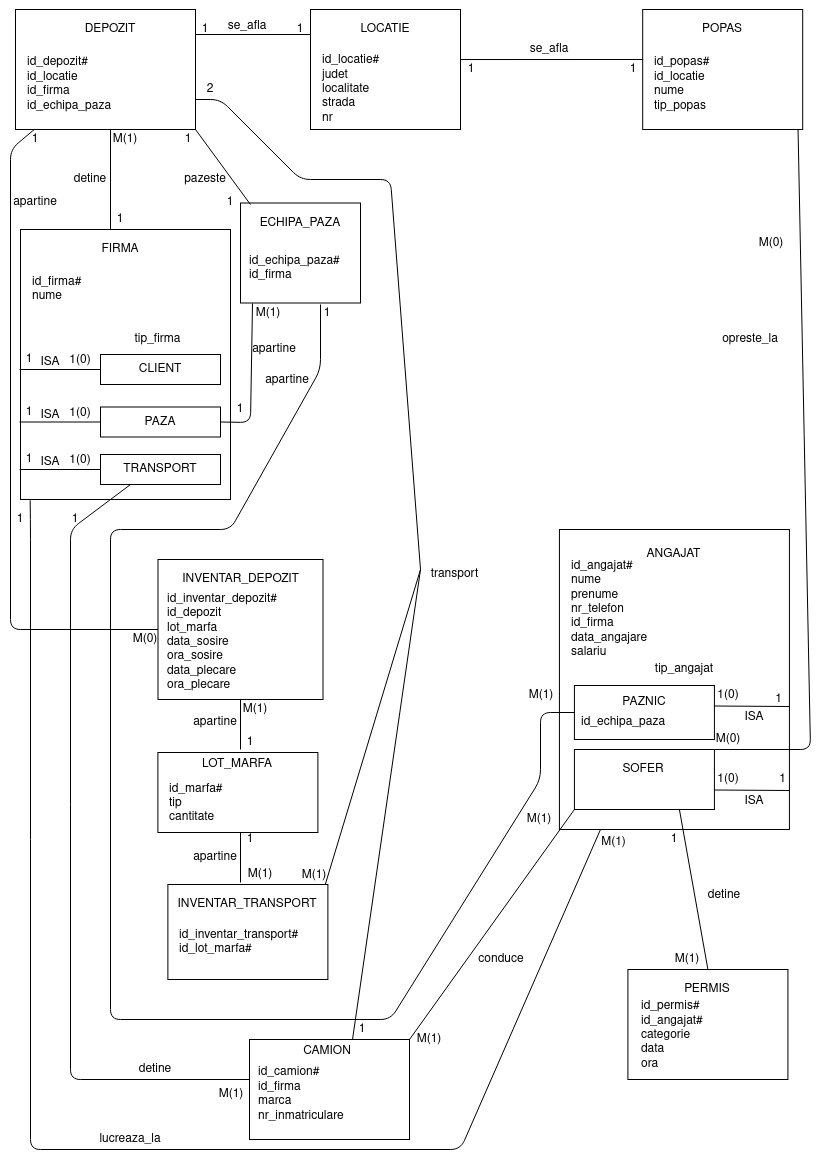
\includegraphics[width=\textwidth]{_diagrama_er.png}
\label{Figura 1}
\centering Figura 1

\justify

\section{Diagrama conceptuală}
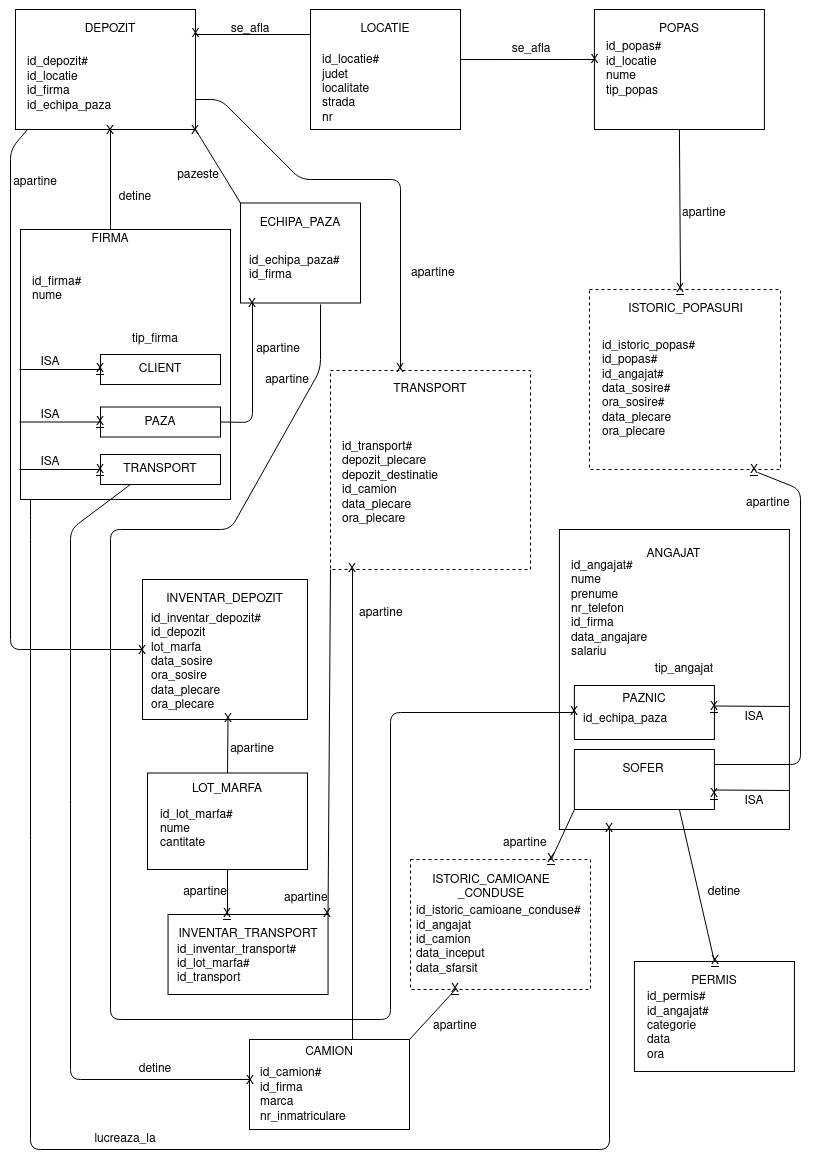
\includegraphics[width=\textwidth]{_diagrama_conceptuala.png}
\label{Figura 2}
\centering Figura 2

\justify

\section{Implementarea diagramei conceptuale}

\begin{lstlisting}[language=SQL]
-- crearea tabelelor 

CREATE TABLE LOCATIE
    (id_locatie number(10) constraint pk_loc primary key,
     judet varchar2(25),
     localitate varchar2(25),
     strada varchar2(25),
     nr number(5)
     );
     
CREATE TABLE POPAS
    (id_popas number(10) constraint pk_pop primary key,
     id_locatie number(10) constraint fk_pop_loc references 
                                LOCATIE(id_locatie) on delete set null,
     nume varchar2(25),
     tip_popas varchar2(10) constraint tip_pop not null,
     constraint verif_tip_pop check(tip_popas = 'BENZINARIE' 
                            or tip_popas = 'MOTEL' or tip_popas = 'RESTAURANT')
     );
     
CREATE TABLE FIRMA
    (id_firma number(12) constraint pk_firma primary key,
     nume varchar2(25) constraint uni_nume_firma unique,
     tip_firma varchar2(10) constraint tip_firma not null,
     constraint verif_tip_firma check(tip_firma = 'CLIENT' or tip_firma = 'PAZA'
                                        or tip_firma = 'TRANSPORT')
     );
     
CREATE TABLE ECHIPA_PAZA
    (id_echipa_paza number(5) constraint pk_epaza primary key,
     id_firma number(12) constraint fk_epaza_firma references 
                            FIRMA(id_firma) on delete cascade
     );
     
CREATE TABLE DEPOZIT
    (id_depozit number(5) constraint pk_dep primary key,
     id_locatie number(5) constraint fk_dep_loc references 
                            LOCATIE(id_locatie) on delete set null,
     id_echipa_paza number(5) constraint fk_dep_epaza 
                references ECHIPA_PAZA(id_echipa_paza) on delete set null,
     id_firma number(12) constraint fk_dep_firma references FIRMA(id_firma) 
                            on delete set null
     );

CREATE TABLE CAMION
    (id_camion number(5) constraint pk_cam primary key,
     marca varchar2(10),
     nr_inmatriculare varchar2(10) constraint uni_nr_ing_cam unique,
     id_firma number(12) constraint fk_cam_firma references 
                            FIRMA(id_firma) on delete set null
     );
     
CREATE TABLE TRANSPORT
    (id_transport number(10) constraint pk_trans primary key,
     depozit_plecare number(5) constraint fk_trans_dep_p references 
                                    DEPOZIT(id_depozit) on delete cascade,
     depozit_destinatie number(5) constraint fk_trans_dep_d references 
                                    DEPOZIT(id_depozit) on delete cascade,
     id_camion number(5) constraint fk_trans_cam references 
                            CAMION(id_camion) on delete cascade,
     data_plecare date default sysdate
     );
     
CREATE TABLE LOT_MARFA
    (id_lot_marfa number(10) constraint pk_lotm primary key,
     nume varchar2(25) constraint nume_lotm not null,
     cantitate number(8, 2) constraint cant_lotm not null
     );
     
CREATE TABLE INVENTAR_DEPOZIT
    (id_inventar_depozit number(10) constraint pk_inv_dep primary key,
     id_depozit number(5) constraint fk_invdep_dep references 
                                DEPOZIT(id_depozit) on delete cascade,
     id_lot_marfa number(10) constraint fk_invdep_lotm references 
                                LOT_MARFA(id_lot_marfa) on delete cascade,
     data_sosire date default sysdate,
     data_plecare date
     );
     
CREATE TABLE INVENTAR_TRANSPORT
    (id_inventar_transport number(10),
     id_lot_marfa number(10) constraint fk_invtran_lotm references
                                LOT_MARFA(id_lot_marfa) on delete cascade,
     id_transport number(10) constraint fk_invtran_tran references 
                                TRANSPORT(id_transport) on delete cascade,
     constraint pk_inv_tran primary key(id_inventar_transport, id_lot_marfa)
     );
     
CREATE TABLE ANGAJAT
    (id_angajat number(10) constraint pk_ang primary key,
     nume varchar(25),
     prenume varchar(25),
     nr_telefon varchar(14),
     data_angajare date default sysdate,
     salariu number(10),
     id_firma number(12),
     tip_angajat char(6) constraint tip_ang_nn not null,
     id_echipa_paza number(5),
     constraint verf_tip check(tip_angajat = 'PAZNIC' or tip_angajat = 'SOFER'),
     constraint fk_ang_epaza foreign key(id_echipa_paza) 
        references ECHIPA_PAZA(id_echipa_paza) on delete set null,
     constraint fk_ang_firma foreign key(id_firma) 
        references FIRMA(id_firma) on delete set null
     );
     
CREATE TABLE ISTORIC_CAMIOANE_CONDUSE
    (id_istoric_camioane_conduse number(10) constraint pk_ist_cam primary key,
     id_angajat number(10) constraint fk_icam_ang references 
                            ANGAJAT(id_angajat) on delete cascade,
     id_camion number(5) constraint fk_icam_cam references 
                            CAMION(id_camion) on delete cascade,
     data_inceput date default sysdate,
     data_sfarsit date
     );
     
CREATE TABLE PERMIS
    (id_permis number(10),
     id_angajat number(10) constraint fk_perm_ang references 
                            ANGAJAT(id_angajat) on delete cascade,
     categorie char(3),
     data date default sysdate,
     constraint pk_perm primary key(id_permis, id_angajat),
     constraint verf_catg check(categorie in ('AM', 'A1', 'A2', 'A', 'B1', 'B',
        'BE', 'C1', 'C1E', 'C', 'CE', 'D1', 'D1E', 'D', 'DE', 'Tr', 'Tb', 'Tv'))
     );
     
CREATE TABLE ISTORIC_POPASURI
    (id_istoric_popas number(20),
     id_popas number(10) constraint fk_istpop_pop references POPAS(id_popas),
     id_angajat number(10) constraint fk_istpop_ang references ANGAJAT(id_angajat),
     data_sosire date default sysdate,
     data_plecare date default sysdate,
     constraint pk_ist_pop primary key(id_istoric_popas, id_popas, id_angajat, data_sosire)
     );


/* pentru tabelul Locatie se creeaza urmatoarea secventa SEQ_LOC pentru inserarea
 * inregistrarilor in tabelul Locatie, se va proceda analog pentru celelalte
 * exemple fara a se mai specifica intr-un comentariu */
CREATE SEQUENCE SEQ_LOC
INCREMENT BY 10
START WITH 10
MAXVALUE 1000000000
NOCYCLE;

/* se insereaza date in tabelul Locatie folosind secventa anterior creata
 * utilizandu-se metoda implicita | se va proceda analog pentru inserarea de
 * date in celelalte tabele fara a se mai specifica intr-un comentariu */
INSERT INTO LOCATIE
VALUES(SEQ_LOC.NEXTVAL, 'Prahova', 'Ploiesti', 'Libertatii', 13);

INSERT INTO LOCATIE
VALUES(SEQ_LOC.NEXTVAL, 'Prahova', 'Ploiesti', 'Lalelelor', 142);

INSERT INTO LOCATIE
VALUES(SEQ_LOC.NEXTVAL, 'Prahova', 'Ploiesti', 'Primaverii', 412);

INSERT INTO LOCATIE
VALUES(SEQ_LOC.NEXTVAL, 'Iasi', 'Iasi', 'Unirii', 9991);

INSERT INTO LOCATIE
VALUES(SEQ_LOC.NEXTVAL, 'Iasi', 'Iasi', 'Mihai Eminescu', 991);

INSERT INTO LOCATIE
VALUES(SEQ_LOC.NEXTVAL, 'Iasi', 'Iasi', 'Teilor', 131);

INSERT INTO LOCATIE
VALUES(SEQ_LOC.NEXTVAL, 'Constanta', 'Constanta', 'Teilor', 21);

INSERT INTO LOCATIE
VALUES(SEQ_LOC.NEXTVAL, 'Constanta', 'Constanta', 'Victoriei', 123);

INSERT INTO LOCATIE
VALUES(SEQ_LOC.NEXTVAL, 'Constanta', 'Constanta', 'Zorilor', 13);

INSERT INTO LOCATIE
VALUES(SEQ_LOC.NEXTVAL, 'Tulcea', 'Tulcea', 'Unirii', 213);

INSERT INTO LOCATIE
VALUES(SEQ_LOC.NEXTVAL, 'Tulcea', 'Tulcea', 'Victoriei', 113);

INSERT INTO LOCATIE
VALUES(SEQ_LOC.NEXTVAL, 'Ilfov', 'Bucuresti', 'Libertatii', 112);

INSERT INTO LOCATIE
VALUES(SEQ_LOC.NEXTVAL, 'Ilfov', 'Bucuresti', '1 mai', 1213);

INSERT INTO LOCATIE
VALUES(SEQ_LOC.NEXTVAL, 'Ilfov', 'Bucuresti', 'Muncii', 1412);

INSERT INTO LOCATIE
VALUES(SEQ_LOC.NEXTVAL, 'Ilfov', 'Bucuresti', 'Unirii', 212);

CREATE SEQUENCE SEQ_POP
INCREMENT BY 20
START WITH 100
MAXVALUE 1000000000
NOCYCLE;

INSERT INTO POPAS
VALUES(SEQ_POP.NEXTVAL, 10, 'Motel Sunday', 'MOTEL');

INSERT INTO POPAS
VALUES(SEQ_POP.NEXTVAL, 20, 'Restaurant Ceptura', 'RESTAURANT');

INSERT INTO POPAS
VALUES(SEQ_POP.NEXTVAL, 40, 'Restaurant Grand', 'RESTAURANT');

INSERT INTO POPAS
VALUES(SEQ_POP.NEXTVAL, 60, 'Restaurant Unirea', 'RESTAURANT');

INSERT INTO POPAS
VALUES(SEQ_POP.NEXTVAL, 70, 'Conacul dintre vii', 'MOTEL');

CREATE SEQUENCE SEQ_FIRMA
INCREMENT BY 100
START WITH 100
MAXVALUE 1000000
NOCYCLE;

INSERT INTO FIRMA
VALUES(SEQ_FIRMA.NEXTVAL, 'Lidl', 'CLIENT');

INSERT INTO FIRMA
VALUES(SEQ_FIRMA.NEXTVAL, 'Profi', 'CLIENT');

INSERT INTO FIRMA
VALUES(SEQ_FIRMA.NEXTVAL, 'ABOUT YOU', 'CLIENT');

INSERT INTO FIRMA
VALUES(SEQ_FIRMA.NEXTVAL, 'Deichmann', 'CLIENT');

INSERT INTO FIRMA
VALUES(SEQ_FIRMA.NEXTVAL, 'H and M', 'CLIENT');

INSERT INTO FIRMA
VALUES(SEQ_FIRMA.NEXTVAL, 'STOP SEAL GUARD', 'PAZA');

INSERT INTO FIRMA
VALUES(SEQ_FIRMA.NEXTVAL, 'ATMAN PROTECTION', 'PAZA');

INSERT INTO FIRMA
VALUES(SEQ_FIRMA.NEXTVAL, 'GARDIENII', 'PAZA');

INSERT INTO FIRMA
VALUES(SEQ_FIRMA.NEXTVAL, 'QUICK PROTECT', 'PAZA');

INSERT INTO FIRMA
VALUES(SEQ_FIRMA.NEXTVAL, 'JOHNNY VIP SECURITY', 'PAZA');

INSERT INTO FIRMA
VALUES(SEQ_FIRMA.NEXTVAL, 'Road Logistics', 'TRANSPORT');

INSERT INTO FIRMA
VALUES(SEQ_FIRMA.NEXTVAL, 'Transibo', 'TRANSPORT');

INSERT INTO FIRMA
VALUES(SEQ_FIRMA.NEXTVAL, 'EasyCargo', 'TRANSPORT');

INSERT INTO FIRMA
VALUES(SEQ_FIRMA.NEXTVAL, 'Lextom Trans Asd', 'TRANSPORT');

INSERT INTO FIRMA
VALUES(SEQ_FIRMA.NEXTVAL, 'FedEx', 'TRANSPORT');

INSERT INTO ECHIPA_PAZA
VALUES(1, 600);

INSERT INTO ECHIPA_PAZA
VALUES(2, 600);

INSERT INTO ECHIPA_PAZA
VALUES(3, 800);

INSERT INTO ECHIPA_PAZA
VALUES(4, 700);

INSERT INTO ECHIPA_PAZA
VALUES(5, 900);

INSERT INTO ECHIPA_PAZA
VALUES(6, 1000);

INSERT INTO ECHIPA_PAZA
VALUES(7, 1000);

INSERT INTO ECHIPA_PAZA
VALUES(8, 600);

INSERT INTO ECHIPA_PAZA
VALUES(9, 700);

INSERT INTO ECHIPA_PAZA
VALUES(10, 600);

CREATE SEQUENCE SEQ_DEP
INCREMENT BY 500
START WITH 500
MAXVALUE 50000
NOCYCLE;

INSERT INTO DEPOZIT
VALUES(SEQ_DEP.NEXTVAL, 30, 2, 100);
INSERT INTO DEPOZIT
VALUES(SEQ_DEP.NEXTVAL, 50, 3, 200);
INSERT INTO DEPOZIT
VALUES(SEQ_DEP.NEXTVAL, 80, 1, 300);
INSERT INTO DEPOZIT
VALUES(SEQ_DEP.NEXTVAL, 90, 5, 400);
INSERT INTO DEPOZIT
VALUES(SEQ_DEP.NEXTVAL, 110, 6, 500);
INSERT INTO DEPOZIT
VALUES(SEQ_DEP.NEXTVAL, 100, 4, 1100);
INSERT INTO DEPOZIT
VALUES(SEQ_DEP.NEXTVAL, 120, 10, 1200);
INSERT INTO DEPOZIT
VALUES(SEQ_DEP.NEXTVAL, 140, 8, 1300);
INSERT INTO DEPOZIT
VALUES(SEQ_DEP.NEXTVAL, 150, 7, 1400);
INSERT INTO DEPOZIT
VALUES(SEQ_DEP.NEXTVAL, 130, 9, 1500);

CREATE SEQUENCE SEQ_CAM
INCREMENT BY 10
START WITH 15
MAXVALUE 10000
NOCYCLE;

INSERT INTO CAMION
VALUES(SEQ_CAM.NEXTVAL, 'VOLVO', 'CT12FSD', 1100);

INSERT INTO CAMION
VALUES(SEQ_CAM.NEXTVAL, 'VOLVO', 'CT90MMM', 1100);

INSERT INTO CAMION
VALUES(SEQ_CAM.NEXTVAL, 'SCANIA', 'PH13SCN', 1200);

INSERT INTO CAMION
VALUES(SEQ_CAM.NEXTVAL, 'DAF', 'B55ASD', 1300);

INSERT INTO CAMION
VALUES(SEQ_CAM.NEXTVAL, 'IVECO', 'MM13IVC', 1400);

INSERT INTO CAMION
VALUES(SEQ_CAM.NEXTVAL, 'MAN', 'TM20QWE', 1100);

INSERT INTO CAMION
VALUES(SEQ_CAM.NEXTVAL, 'SCANIA', 'IS32ISA', 1100);

INSERT INTO CAMION
VALUES(SEQ_CAM.NEXTVAL, 'MAN', 'IS01MAN', 1200);

INSERT INTO CAMION
VALUES(SEQ_CAM.NEXTVAL,'DAF', 'TM11IOP', 1300);

INSERT INTO CAMION
VALUES(SEQ_CAM.NEXTVAL, 'VOLVO', 'MM57RXF', 1500);

INSERT INTO CAMION
VALUES(SEQ_CAM.NEXTVAL, 'SCANIA', 'B29SCN', 1500);

CREATE SEQUENCE SEQ_TRAN
INCREMENT BY 10
START WITH 10000
MAXVALUE 2000000000
NOCYCLE;

INSERT INTO TRANSPORT
VALUES(SEQ_TRAN.NEXTVAL, 3000, 500, 15, to_date('06-05-2021 08:00', 'dd-mm-yyyy, hh24:mi'));

INSERT INTO TRANSPORT
VALUES(SEQ_TRAN.NEXTVAL, 3000, 500, 25, to_date('08-05-2021 06:00', 'dd-mm-yyyy, hh24:mi'));

INSERT INTO TRANSPORT
VALUES(SEQ_TRAN.NEXTVAL, 3500, 1000, 35, to_date('06-05-2021 08:00', 'dd-mm-yyyy, hh24:mi'));

INSERT INTO TRANSPORT
VALUES(SEQ_TRAN.NEXTVAL, 4000, 1000, 45, to_date('06-05-2021 06:00', 'dd-mm-yyyy, hh24:mi'));

INSERT INTO TRANSPORT
VALUES(SEQ_TRAN.NEXTVAL, 4500, 1000, 55, to_date('06-05-2021 06:00', 'dd-mm-yyyy, hh24:mi'));

INSERT INTO TRANSPORT
VALUES(SEQ_TRAN.NEXTVAL, 5000, 1500, 115, to_date('07-05-2021 08:00', 'dd-mm-yyyy, hh24:mi'));

INSERT INTO TRANSPORT
VALUES(SEQ_TRAN.NEXTVAL, 5000, 1500, 105, to_date('05-05-2021 06:00', 'dd-mm-yyyy, hh24:mi'));

INSERT INTO TRANSPORT
VALUES(SEQ_TRAN.NEXTVAL, 3500, 2000, 85, to_date('06-05-2021 06:00', 'dd-mm-yyyy, hh24:mi'));

INSERT INTO TRANSPORT
VALUES(SEQ_TRAN.NEXTVAL, 3500, 2000, 85, to_date('07-05-2021 06:00', 'dd-mm-yyyy, hh24:mi'));

INSERT INTO TRANSPORT
VALUES(SEQ_TRAN.NEXTVAL, 3000, 2500, 25, to_date('10-05-2021 07:00', 'dd-mm-yyyy, hh24:mi'));

INSERT INTO TRANSPORT
VALUES(SEQ_TRAN.NEXTVAL, 3000, 2500, 15, to_date('11-05-2021 05:00', 'dd-mm-yyyy, hh24:mi'));

CREATE SEQUENCE SEQ_LOTM
INCREMENT BY 5
START WITH 100
MAXVALUE 5000000000
NOCYCLE;

INSERT INTO LOT_MARFA
VALUES(SEQ_LOTM.NEXTVAL, 'carne miel', 100.00);

INSERT INTO LOT_MARFA
VALUES(SEQ_LOTM.NEXTVAL, 'carne porc', 300.00);

INSERT INTO LOT_MARFA
VALUES(SEQ_LOTM.NEXTVAL, 'carne pui', 250.00);

INSERT INTO LOT_MARFA
VALUES(SEQ_LOTM.NEXTVAL, 'carne pui', 200.00);

INSERT INTO LOT_MARFA
VALUES(SEQ_LOTM.NEXTVAL, 'rosii', 1000.00);

INSERT INTO LOT_MARFA
VALUES(SEQ_LOTM.NEXTVAL, 'rosii', 1500.00);

INSERT INTO LOT_MARFA
VALUES(SEQ_LOTM.NEXTVAL, 'ardei', 500.00);

INSERT INTO LOT_MARFA
VALUES(SEQ_LOTM.NEXTVAL, 'lapte', 100.00);

INSERT INTO LOT_MARFA
VALUES(SEQ_LOTM.NEXTVAL, 'lapte', 100.00);

INSERT INTO LOT_MARFA
VALUES(SEQ_LOTM.NEXTVAL, 'lapte', 120.00);

INSERT INTO LOT_MARFA
VALUES(SEQ_LOTM.NEXTVAL, 'tricouri', 100.00);

INSERT INTO LOT_MARFA
VALUES(SEQ_LOTM.NEXTVAL, 'tricouri', 90.00);

INSERT INTO LOT_MARFA
VALUES(SEQ_LOTM.NEXTVAL, 'tricouri', 10.00);

INSERT INTO LOT_MARFA
VALUES(SEQ_LOTM.NEXTVAL, 'pantofi', 20.00);

INSERT INTO LOT_MARFA
VALUES(SEQ_LOTM.NEXTVAL, 'pantofi', 30.00);

INSERT INTO LOT_MARFA
VALUES(SEQ_LOTM.NEXTVAL, 'hanorace', 50.00);

INSERT INTO LOT_MARFA
VALUES(SEQ_LOTM.NEXTVAL, 'hanorace', 35.00);

INSERT INTO LOT_MARFA
VALUES(SEQ_LOTM.NEXTVAL, 'rochii', 50.00);

INSERT INTO LOT_MARFA
VALUES(SEQ_LOTM.NEXTVAL, 'fuste', 35.00);

INSERT INTO LOT_MARFA
VALUES(SEQ_LOTM.NEXTVAL, 'blugi', 35.00);

CREATE SEQUENCE SEQ_INV_DEP
INCREMENT BY 50
START WITH 100
MAXVALUE 500000000
NOCYCLE;

--10040
INSERT INTO INVENTAR_DEPOZIT
VALUES(SEQ_INV_DEP.NEXTVAL, 3000, 100, to_date('02-04-2021 12:00', 'dd-mm-yyyy hh24:mi'), null);
--10040
INSERT INTO INVENTAR_DEPOZIT
VALUES(SEQ_INV_DEP.NEXTVAL, 3000, 105, to_date('02-04-2021 10:00', 'dd-mm-yyyy hh24:mi'), null);
--10050
INSERT INTO INVENTAR_DEPOZIT
VALUES(SEQ_INV_DEP.NEXTVAL, 3000, 110, to_date('01-04-2021 11:00', 'dd-mm-yyyy hh24:mi'), null);

INSERT INTO INVENTAR_DEPOZIT
VALUES(SEQ_INV_DEP.NEXTVAL, 3000, 115, to_date('25-04-2021 12:00', 'dd-mm-yyyy hh24:mi'), null);

--10060
INSERT INTO INVENTAR_DEPOZIT
VALUES(SEQ_INV_DEP.NEXTVAL, 3500, 120, to_date('24-04-2021 12:00', 'dd-mm-yyyy hh24:mi'), null);
INSERT INTO INVENTAR_DEPOZIT
VALUES(SEQ_INV_DEP.NEXTVAL, 3500, 130, to_date('07-04-2021 12:00', 'dd-mm-yyyy hh24:mi'), null);

--10070
INSERT INTO INVENTAR_DEPOZIT
VALUES(SEQ_INV_DEP.NEXTVAL, 4000, 140, to_date('12-04-2021 12:00', 'dd-mm-yyyy hh24:mi'), null);

--10080
INSERT INTO INVENTAR_DEPOZIT
VALUES(SEQ_INV_DEP.NEXTVAL, 4500, 125, to_date('21-04-2021 12:00', 'dd-mm-yyyy hh24:mi'), null);
INSERT INTO INVENTAR_DEPOZIT
VALUES(SEQ_INV_DEP.NEXTVAL, 4500, 145, to_date('13-04-2021 12:00', 'dd-mm-yyyy hh24:mi'), null);

--10090
INSERT INTO INVENTAR_DEPOZIT
VALUES(SEQ_INV_DEP.NEXTVAL, 5000, 195, to_date('11-04-2021 12:00', 'dd-mm-yyyy hh24:mi'), null);

--10100
INSERT INTO INVENTAR_DEPOZIT
VALUES(SEQ_INV_DEP.NEXTVAL, 5000, 150, to_date('14-04-2021 12:00', 'dd-mm-yyyy hh24:mi'), null);
INSERT INTO INVENTAR_DEPOZIT
VALUES(SEQ_INV_DEP.NEXTVAL, 5000, 175, to_date('02-04-2021 12:00', 'dd-mm-yyyy hh24:mi'), null);

--10110
INSERT INTO INVENTAR_DEPOZIT
VALUES(SEQ_INV_DEP.NEXTVAL, 3500, 165, to_date('03-04-2021 12:00', 'dd-mm-yyyy hh24:mi'), null);

--10120
INSERT INTO INVENTAR_DEPOZIT
VALUES(SEQ_INV_DEP.NEXTVAL, 3500, 170, to_date('02-04-2021 12:00', 'dd-mm-yyyy hh24:mi'), null);

--10130
INSERT INTO INVENTAR_DEPOZIT
VALUES(SEQ_INV_DEP.NEXTVAL, 3000, 190, to_date('06-04-2021 12:00', 'dd-mm-yyyy hh24:mi'), null);
INSERT INTO INVENTAR_DEPOZIT
VALUES(SEQ_INV_DEP.NEXTVAL, 3000, 185, to_date('01-04-2021 12:00', 'dd-mm-yyyy hh24:mi'), null);

--10140
INSERT INTO INVENTAR_DEPOZIT
VALUES(SEQ_INV_DEP.NEXTVAL, 3000, 180, to_date('15-04-2021 12:00', 'dd-mm-yyyy hh24:mi'), null);

INSERT INTO INVENTAR_DEPOZIT
VALUES(SEQ_INV_DEP.NEXTVAL, 5000, 160, to_date('11-04-2021 12:00', 'dd-mm-yyyy hh24:mi'), null);
INSERT INTO INVENTAR_DEPOZIT
VALUES(SEQ_INV_DEP.NEXTVAL, 5000, 155, to_date('11-04-2021 12:00', 'dd-mm-yyyy hh24:mi'), null);
INSERT INTO INVENTAR_DEPOZIT
VALUES(SEQ_INV_DEP.NEXTVAL, 5000, 135, to_date('11-04-2021 12:00', 'dd-mm-yyyy hh24:mi'), null);


CREATE SEQUENCE SEQ_INV_TRAN
INCREMENT BY 55
START WITH 100
MAXVALUE 500000000
NOCYCLE;

INSERT INTO INVENTAR_TRANSPORT
VALUES(SEQ_INV_TRAN.NEXTVAL, 100, 10000);
INSERT INTO INVENTAR_TRANSPORT
VALUES(SEQ_INV_TRAN.NEXTVAL, 105, 10000);

INSERT INTO INVENTAR_TRANSPORT
VALUES(SEQ_INV_TRAN.NEXTVAL, 110, 10010);

INSERT INTO INVENTAR_TRANSPORT
VALUES(SEQ_INV_TRAN.NEXTVAL, 120, 10020);
INSERT INTO INVENTAR_TRANSPORT
VALUES(SEQ_INV_TRAN.NEXTVAL, 130, 10020);

INSERT INTO INVENTAR_TRANSPORT
VALUES(SEQ_INV_TRAN.NEXTVAL, 140, 10030);

INSERT INTO INVENTAR_TRANSPORT
VALUES(SEQ_INV_TRAN.NEXTVAL, 125, 10040);
INSERT INTO INVENTAR_TRANSPORT
VALUES(SEQ_INV_TRAN.NEXTVAL, 145, 10040);

INSERT INTO INVENTAR_TRANSPORT
VALUES(SEQ_INV_TRAN.NEXTVAL, 195, 10050);

INSERT INTO INVENTAR_TRANSPORT
VALUES(SEQ_INV_TRAN.NEXTVAL, 150, 10060);
INSERT INTO INVENTAR_TRANSPORT
VALUES(SEQ_INV_TRAN.NEXTVAL, 175, 10060);

INSERT INTO INVENTAR_TRANSPORT
VALUES(SEQ_INV_TRAN.NEXTVAL, 165, 10070);

INSERT INTO INVENTAR_TRANSPORT
VALUES(SEQ_INV_TRAN.NEXTVAL, 170, 10080);

INSERT INTO INVENTAR_TRANSPORT
VALUES(SEQ_INV_TRAN.NEXTVAL, 190, 10090);
INSERT INTO INVENTAR_TRANSPORT
VALUES(SEQ_INV_TRAN.NEXTVAL, 185, 10090);

INSERT INTO INVENTAR_TRANSPORT
VALUES(SEQ_INV_TRAN.NEXTVAL, 180, 10100);

CREATE SEQUENCE SEQ_ANG
INCREMENT BY 20
START WITH 20000
MAXVALUE 2000000000
NOCYCLE;

INSERT INTO ANGAJAT
VALUES(SEQ_ANG.NEXTVAL, 'Ion', 'Vasile', '0722123456', 
    to_date('11-04-2020 12:00', 'dd-mm-yyyy hh24:mi'), 5000, 1100, 'SOFER', null);

INSERT INTO ANGAJAT
VALUES(SEQ_ANG.NEXTVAL, 'Ovidiu', 'Ion', '0727124356', 
    to_date('12-05-2020 12:00', 'dd-mm-yyyy hh24:mi'), 4000, 1100, 'SOFER', null);
    
INSERT INTO ANGAJAT
VALUES(SEQ_ANG.NEXTVAL, 'Popescu', 'Andrei', '0723323465', 
    to_date('11-03-2020 12:00', 'dd-mm-yyyy hh24:mi'), 6000, 1200, 'SOFER', null);
    
INSERT INTO ANGAJAT
VALUES(SEQ_ANG.NEXTVAL, 'Marian', 'Gheorghe', '0721213456', 
    to_date('11-11-2020 12:00', 'dd-mm-yyyy hh24:mi'), 3000, 1200, 'SOFER', null);
    
INSERT INTO ANGAJAT
VALUES(SEQ_ANG.NEXTVAL, 'Manea', 'George', '0721123959', 
    to_date('03-03-2020 12:00', 'dd-mm-yyyy hh24:mi'), 4000, 1300, 'SOFER', null);
    
INSERT INTO ANGAJAT
VALUES(SEQ_ANG.NEXTVAL, 'Constantin', 'Gheorghe', '0735123456', 
    to_date('09-04-2020 12:00', 'dd-mm-yyyy hh24:mi'), 4500, 1400, 'SOFER', null);
    
INSERT INTO ANGAJAT
VALUES(SEQ_ANG.NEXTVAL, 'Ion', 'Catalin', '0721126566', 
    to_date('02-07-2020 12:00', 'dd-mm-yyyy hh24:mi'), 3400, 1500, 'SOFER', null);

INSERT INTO ANGAJAT
VALUES(SEQ_ANG.NEXTVAL, 'Marius', 'Catalin', '072119356', 
    to_date('02-07-2020 12:00', 'dd-mm-yyyy hh24:mi'), 3300, 600, 'PAZNIC', 1);
INSERT INTO ANGAJAT
VALUES(SEQ_ANG.NEXTVAL, 'Grant', 'Ion', '0723123456', 
    to_date('02-07-2020 12:00', 'dd-mm-yyyy hh24:mi'), 3100, 600, 'PAZNIC', 1);

INSERT INTO ANGAJAT
VALUES(SEQ_ANG.NEXTVAL, 'Ivan', 'George', '0726100456', 
    to_date('02-07-2020 12:00', 'dd-mm-yyyy hh24:mi'), 3250, 600, 'PAZNIC', 2);

INSERT INTO ANGAJAT
VALUES(SEQ_ANG.NEXTVAL, 'Neagu', 'Ion', '0728123456', 
    to_date('02-07-2020 12:00', 'dd-mm-yyyy hh24:mi'), 3500, 800, 'PAZNIC', 3);

INSERT INTO ANGAJAT
VALUES(SEQ_ANG.NEXTVAL, 'Popescu', 'Cristian', '0724523456', 
    to_date('02-07-2020 12:00', 'dd-mm-yyyy hh24:mi'), 3600, 700, 'PAZNIC', 4);

INSERT INTO ANGAJAT
VALUES(SEQ_ANG.NEXTVAL, 'Marius', 'Mihai', '0721223456', 
    to_date('02-07-2020 12:00', 'dd-mm-yyyy hh24:mi'), 3450, 900, 'PAZNIC', 5);

INSERT INTO ANGAJAT
VALUES(SEQ_ANG.NEXTVAL, 'Radu', 'Gheorghe', '0724323456', 
    to_date('02-07-2020 12:00', 'dd-mm-yyyy hh24:mi'), 3375, 1000, 'PAZNIC', 6);

INSERT INTO ANGAJAT
VALUES(SEQ_ANG.NEXTVAL, 'Marin', 'Catalin', '0725623456', 
    to_date('02-07-2020 12:00', 'dd-mm-yyyy hh24:mi'), 3150, 1000, 'PAZNIC', 7);

INSERT INTO ANGAJAT
VALUES(SEQ_ANG.NEXTVAL, 'Andrei', 'David', '0722123456', 
    to_date('02-07-2020 12:00', 'dd-mm-yyyy hh24:mi'), 3250, 600, 'PAZNIC', 8);

INSERT INTO ANGAJAT
VALUES(SEQ_ANG.NEXTVAL, 'Popescu', 'Stefan', '0721145456', 
    to_date('02-07-2020 12:00', 'dd-mm-yyyy hh24:mi'), 3400, 700, 'PAZNIC', 9);

INSERT INTO ANGAJAT
VALUES(SEQ_ANG.NEXTVAL, 'Ion', 'Catalin', '0721765456', 
    to_date('02-07-2020 12:00', 'dd-mm-yyyy hh24:mi'), 3320, 600, 'PAZNIC', 10);
         
CREATE SEQUENCE SEQ_IST_CAM
INCREMENT BY 5
START WITH 5
MAXVALUE 2000000000
NOCYCLE;

INSERT INTO ISTORIC_CAMIOANE_CONDUSE
VALUES(SEQ_IST_CAM.NEXTVAL, 20000, 65, to_date('11-04-2020 12:00', 'dd-mm-yyyy hh24:mi'), 
    to_date('13-07-2020 12:00', 'dd-mm-yyyy hh24:mi'));

INSERT INTO ISTORIC_CAMIOANE_CONDUSE
VALUES(SEQ_IST_CAM.NEXTVAL, 20000, 75, to_date('13-07-2020 12:00', 'dd-mm-yyyy hh24:mi'), 
    to_date('21-11-2020 12:00', 'dd-mm-yyyy hh24:mi'));

INSERT INTO ISTORIC_CAMIOANE_CONDUSE
VALUES(SEQ_IST_CAM.NEXTVAL, 20000, 15, to_date('21-11-2020 12:00', 'dd-mm-yyyy hh24:mi'), null);

INSERT INTO ISTORIC_CAMIOANE_CONDUSE
VALUES(SEQ_IST_CAM.NEXTVAL, 20020, 25, to_date('12-05-2020 12:00', 'dd-mm-yyyy hh24:mi'), null);

INSERT INTO ISTORIC_CAMIOANE_CONDUSE
VALUES(SEQ_IST_CAM.NEXTVAL, 20040, 85, to_date('11-03-2020 12:00', 'dd-mm-yyyy hh24:mi'), null);

INSERT INTO ISTORIC_CAMIOANE_CONDUSE
VALUES(SEQ_IST_CAM.NEXTVAL, 20060, 35, to_date('11-11-2020 12:00', 'dd-mm-yyyy hh24:mi'), null);

INSERT INTO ISTORIC_CAMIOANE_CONDUSE
VALUES(SEQ_IST_CAM.NEXTVAL, 20080, 45, to_date('03-03-2020 12:00', 'dd-mm-yyyy hh24:mi'), null);

INSERT INTO ISTORIC_CAMIOANE_CONDUSE
VALUES(SEQ_IST_CAM.NEXTVAL, 20100, 55, to_date('09-04-2020 12:00', 'dd-mm-yyyy hh24:mi'), null);

INSERT INTO ISTORIC_CAMIOANE_CONDUSE
VALUES(SEQ_IST_CAM.NEXTVAL, 20120, 105, to_date('02-07-2020 12:00', 'dd-mm-yyyy hh24:mi'), 
        to_date('06-06-2020 12:00', 'dd-mm-yyyy hh24:mi'));

INSERT INTO ISTORIC_CAMIOANE_CONDUSE
VALUES(SEQ_IST_CAM.NEXTVAL, 20120, 115, to_date('06-06-2020 12:00', 'dd-mm-yyyy hh24:mi'), null);

CREATE SEQUENCE SEQ_PERM
INCREMENT BY 2
START WITH 1
MAXVALUE 1000000000
NOCYCLE;

INSERT INTO PERMIS
VALUES(SEQ_PERM.NEXTVAL, 20000,'C', to_date('06-06-2017 12:00', 'dd-mm-yyyy hh24:mi'));

INSERT INTO PERMIS
VALUES(SEQ_PERM.NEXTVAL, 20000,'A', to_date('06-06-2013 12:00', 'dd-mm-yyyy hh24:mi'));

INSERT INTO PERMIS
VALUES(SEQ_PERM.NEXTVAL, 20000,'B', to_date('06-06-2012 12:00', 'dd-mm-yyyy hh24:mi'));

INSERT INTO PERMIS
VALUES(SEQ_PERM.NEXTVAL, 20020,'C', to_date('06-06-2018 12:00', 'dd-mm-yyyy hh24:mi'));

INSERT INTO PERMIS
VALUES(SEQ_PERM.NEXTVAL, 20040,'C', to_date('06-05-2016 12:00', 'dd-mm-yyyy hh24:mi'));

INSERT INTO PERMIS
VALUES(SEQ_PERM.NEXTVAL, 20060,'C', to_date('03-11-2014 12:00', 'dd-mm-yyyy hh24:mi'));

INSERT INTO PERMIS
VALUES(SEQ_PERM.NEXTVAL, 20080,'C', to_date('03-03-2002 12:00', 'dd-mm-yyyy hh24:mi'));

INSERT INTO PERMIS
VALUES(SEQ_PERM.NEXTVAL, 20100,'B', to_date('06-11-2010 12:00', 'dd-mm-yyyy hh24:mi'));

INSERT INTO PERMIS
VALUES(SEQ_PERM.NEXTVAL, 20100,'C', to_date('06-11-2012 12:00', 'dd-mm-yyyy hh24:mi'));

INSERT INTO PERMIS
VALUES(SEQ_PERM.NEXTVAL, 20120,'C', to_date('12-06-2014 12:00', 'dd-mm-yyyy hh24:mi'));

CREATE SEQUENCE SEQ_IST_POP
INCREMENT BY 5
START WITH 50
MAXVALUE 10000000000000000000
NOCYCLE;

INSERT INTO ISTORIC_POPASURI
VALUES(SEQ_IST_POP.NEXTVAL, 180, 20000, to_date('06-05-2021 10:00', 'dd-mm-yyyy hh24:mi'), to_date('06-05-2021 12:00', 'dd-mm-yyyy hh24:mi'));

INSERT INTO ISTORIC_POPASURI
VALUES(SEQ_IST_POP.NEXTVAL, 120, 20000, to_date('06-05-2021 21:00', 'dd-mm-yyyy hh24:mi'), to_date('06-05-2021 21:30', 'dd-mm-yyyy hh24:mi'));

INSERT INTO ISTORIC_POPASURI
VALUES(SEQ_IST_POP.NEXTVAL, 180, 20020, to_date('08-05-2021 10:00', 'dd-mm-yyyy hh24:mi'), to_date('08-05-2021 12:00', 'dd-mm-yyyy hh24:mi'));

INSERT INTO ISTORIC_POPASURI
VALUES(SEQ_IST_POP.NEXTVAL, 120, 20020, to_date('08-05-2021 21:00', 'dd-mm-yyyy hh24:mi'), to_date('08-05-2021 21:30', 'dd-mm-yyyy hh24:mi'));

INSERT INTO ISTORIC_POPASURI
VALUES(SEQ_IST_POP.NEXTVAL, 100, 20060, to_date('06-05-2021 10:00', 'dd-mm-yyyy hh24:mi'), to_date('06-05-2021 10:20', 'dd-mm-yyyy hh24:mi'));

INSERT INTO ISTORIC_POPASURI
VALUES(SEQ_IST_POP.NEXTVAL, 140, 20060, to_date('06-05-2021 19:00', 'dd-mm-yyyy hh24:mi'), to_date('06-05-2021 19:30', 'dd-mm-yyyy hh24:mi'));

INSERT INTO ISTORIC_POPASURI
VALUES(SEQ_IST_POP.NEXTVAL, 140, 20080, to_date('06-05-2021 17:00', 'dd-mm-yyyy hh24:mi'), to_date('06-05-2021 17:30', 'dd-mm-yyyy hh24:mi'));

INSERT INTO ISTORIC_POPASURI
VALUES(SEQ_IST_POP.NEXTVAL, 140, 20100, to_date('06-05-2021 17:00', 'dd-mm-yyyy hh24:mi'), to_date('06-05-2021 17:30', 'dd-mm-yyyy hh24:mi'));

INSERT INTO ISTORIC_POPASURI
VALUES(SEQ_IST_POP.NEXTVAL, 180, 20120, to_date('07-05-2021 17:00', 'dd-mm-yyyy hh24:mi'), to_date('07-05-2021 17:30', 'dd-mm-yyyy hh24:mi'));

INSERT INTO ISTORIC_POPASURI
VALUES(SEQ_IST_POP.NEXTVAL, 180, 20120, to_date('05-05-2021 17:00', 'dd-mm-yyyy hh24:mi'), to_date('05-05-2021 17:30', 'dd-mm-yyyy hh24:mi'));

commit; -- salvam inserarile
\end{lstlisting}

\section{Probleme rezolvate de baza de date}

Afisati pentru toti soferi toate popasurile in care s-au oprit in ziua in care
s-a oprit pentru prima data un sofer la restaurantul Ceptura din Ploiesti, sa
se afiseze daca soferul a venit cu un camion inmatriculat in Prahova sau in
alta regiune, numele, prenumele si salariul soferului, numele si tipul
popasului la care s-a oprit, la ce ora a sosit, cat a stat, cati bani a
cheltuit la popas, si locatia popasului. Locatia sa fie afisata pe o singura
coloana numita Locatie popas. Un sofer cheltuieste la un popas in functie de
salariul sau, soferii cu un salariu mai mic de 3000lei inclusiv vor cheltui doar
0.005\% din salariu, cei cu salariu intre (3000, 4500] vor chelui 0.01\% din
salariu, iar restul vor cheltui 0.015\% din salariu. Sa se ordoneze dupa nume
si dupa prenume. Din lista de angajati nu afisati nimic pentru ultimii doi din lista.

\begin{lstlisting}[language=SQL]
-- functie pentru a obtine ziua in care s-a oprit pentru prima data un sofer
-- la restaurantul un popas cu numele si locatia data
CREATE OR REPLACE FUNCTION func_obtine_data(
    p_nume_popas popas.nume%type, p_localitate locatie.localitate%TYPE)
RETURN varchar2
    AS v_data_rez varchar2(255);
BEGIN
    SELECT to_char(min(sip.data_sosire), 'dd-mm-yyyy')
    INTO v_data_rez
    FROM locatie sl JOIN popas sp ON (sl.id_locatie = sp.id_locatie)
                    JOIN istoric_popasuri sip ON(sp.id_popas = sip.id_popas)
    WHERE initcap(sp.nume) = p_nume_popas and initcap(sl.localitate) = p_localitate;
    
    return v_data_rez;
END;

-- subprogram pentru a rezolva cerinta data (am ales procedura intrucat nu trebuie
-- sa intoarcem nimic) - folosim o procedura cu 2 parametrii de intrare(default 
-- sunt de intrare setati) pentru a rezolva cerinta la un caz mai general (indiferent
-- de popas)
CREATE OR REPLACE PROCEDURE proc_track_sofer(
    p_nume_popas popas.nume%type, p_localitate locatie.localitate%TYPE)
AS
    -- record pentru a retine date despre soferi (folosim tipurile de date din
    -- tabelul de angajati)
    TYPE rec_sofer_info IS RECORD (
        id_angajat     angajat.id_angajat%TYPE,
        nume           angajat.nume%TYPE,
        prenume        angajat.prenume%TYPE,
        salariu        angajat.salariu%TYPE,
        bani_cheltuiti angajat.salariu%TYPE
    );
    
    -- tabel indexat (INTEGER) cu model de date de tipul record rec_sofer_info
    TYPE t_sofer_info IS TABLE OF rec_sofer_info INDEX BY PLS_INTEGER;
    
    -- record pentru tracking al soferului la un popas
    TYPE rec_track_info IS RECORD (
        din_ph  varchar2(255),
        nume_popas popas.nume%TYPE,
        tip_popas popas.tip_popas%TYPE,
        ora_sosire varchar2(255),
        durata varchar2(255),
        locatie_popas varchar2(255)
    );
    -- tabel imbricat cu model de date de tipul record rec_track_info
    TYPE t_track_info IS TABLE OF rec_track_info;
    
    -- tabel indexat in care vom retine soferi in functie de criteriul stabilit
    t_soferi t_sofer_info;
    -- tabel imbricat care va retine date de tracking pt sofer
    t_track  t_track_info;
    -- data primei opriri a unui sofer la Restaurantul Ceptura din Ploiesti
    v_data   varchar2(255);
    -- pentru a prinde exceptiile de orice fel (in principiu pentru exceptiile aplicatiei)
    exceptie EXCEPTION;
    PRAGMA EXCEPTION_INIT(exceptie, -20001);
    
    -- cursor clasic pentru a obtine informatii despre toti soferii
    CURSOR c_obtine_soferi IS
        SELECT id_angajat, nume, prenume, salariu,
            CASE WHEN salariu <=3000 THEN salariu * 0.005
                 WHEN salariu <=4500 THEN salariu * 0.01
                 WHEN salariu > 4500 THEN salariu * 0.015
            END 
        FROM angajat
        WHERE tip_angajat = 'SOFER' -- vrem doar soferii din toti angajatii
        ORDER BY nume, prenume; -- ordoneaza soferii crescator dupa nume si prenume
    
    -- cursor parametrizat pentru a obtine date de tracking despre un sofer dat dupa id-ul de angajat
    CURSOR c_track(cp_id_angajat angajat.id_angajat%TYPE, cp_data varchar2) IS
        SELECT 
			-- decode pentru a verifica nr de inmatriculare al camionului pe care il 
			-- conducea soferul la momentul opririi la popas, primele 2 caractere ne
			-- spun daca a fost inmatriculat in Prahova sau in alta regiune
			DECODE((SELECT upper(substr(sc.nr_inmatriculare, 0, 2))
                       FROM camion sc JOIN istoric_camioane_conduse sic ON(sc.id_camion = sic.id_camion)
                       WHERE sic.id_angajat = cp_id_angajat -- verificam angajatul
							-- verificam sa obtinem camionul pe care il conducea la momentul dat
                            and ip.data_sosire < NVL(sic.data_sfarsit, sysdate)
                            and ip.data_sosire > NVL(sic.data_inceput, sysdate)
            ), 'PH', 'in Prahova', 'din alta regiune') "Verifica camion din Prahova", 
            p.nume "Nume popas", initcap(p.tip_popas) "Tip popas",
            to_char(ip.data_sosire, 'hh24:mi') "Ora sosire",
            substr(numtodsinterval((ip.data_plecare - ip.data_sosire), 'DAY'), 12, 5) "Durata",
            'Jud: ' || NVL(l.judet, '-') || ' Loc: ' || NVL(l.localitate, '-') ||
            ' Str. ' || NVL(l.strada, '-') || ' Nr. ' || NVL(to_char(l.nr), '-') "Locatie popas"
        FROM istoric_popasuri ip JOIN popas p ON(ip.id_popas = p.id_popas)
                                 JOIN locatie l ON(p.id_locatie = l.id_locatie)
		-- pentru angajatul dat ca parametru si orice popas din ziua data
        WHERE ip.id_angajat = cp_id_angajat AND to_char(data_sosire, 'dd-mm-yyyy') = cp_data;
BEGIN
    -- obtinem data ceruta din cerinta - folosim parametrii din procedura 
	-- si ii pasam functiei
    v_data := func_obtine_data(p_nume_popas, p_localitate);
    
    -- daca nu a fost obtinuta o data pentru tracking atunci urmatoarele queries
    -- nu mai au sens
    IF v_data is null THEN
        RAISE_APPLICATION_ERROR(-20001, 'Nu a oprit niciun sofer la locatia data. '
        ||'Daca rezultatul nu este cel asteptat verificati datele de intrare.');
    END IF;
       
    -- obtine toti soferii pentru inceput folosind cursorul clasic
    OPEN c_obtine_soferi; -- deschidem cursorul pentru a obtine date
    FETCH c_obtine_soferi BULK COLLECT INTO t_soferi;
    CLOSE c_obtine_soferi; -- dupa ce am obtinut date nu mai avem nevoie de cursor 
	-- deci il inchidem, analog pentru cel parametrizat de la liniile 137-139
    
    -- din conditia sa nu se ia in considerare ultimii 2 angajati
    -- putem folosi direct COUNT intrucat nu s au realizat modificari in tabloul
    -- indexat momentan deci ultimul element va fi reprezentat de nr COUNT
    -- dupa prima stergerea penultimul element vi fi reprezentat tot de nr COUNT
    -- intrucat al doilea COUNT este diferit de primul COUNT
    -- SECOND_COUNT = FIRST_COUNT - 1;
    t_soferi.DELETE(t_soferi.COUNT);
    t_soferi.DELETE(t_soferi.COUNT);

-- simulam cazul in care nu am obtinut soferii
--    t_soferi.DELETE();
--    IF t_soferi.COUNT() = 0 THEN
--        RAISE_APPLICATION_ERROR(-20002, 'Nu s-au putut obtine soferii');
--    END IF;

    FOR i IN t_soferi.FIRST..t_soferi.LAST LOOP
        IF t_soferi.EXISTS(i) THEN -- daca exista angajatul
        
        -- obtine informatii despre tracking pentru soferul curent din loop
        OPEN c_track(t_soferi(i).id_angajat, v_data);
        FETCH c_track BULK COLLECT INTO t_track;
        CLOSE c_track;
        
        -- afiseaza date despre sofer
        DBMS_OUTPUT.PUT_LINE('Soferul '||t_soferi(i).prenume||' '||t_soferi(i).nume||' are salariul de '
            ||t_soferi(i).salariu||' de lei si cheltuie in medie '||t_soferi(i).bani_cheltuiti||' lei '
            ||'la un popas. Informatii de tracking:');
         
        -- soferul curent nu s a oprit la niciun popas in ziua respectiva
        -- nu vrem sa aruncam o exceptie ci sa afisam un mesaj explicit pentru acest caz special
        IF t_track.COUNT() = 0 THEN
            DBMS_OUTPUT.PUT_LINE('Nu s-a oprit la niciun popas in data de '||v_data);
        ELSE
            FOR j IN t_track.FIRST..t_track.LAST LOOP
                DBMS_OUTPUT.PUT_LINE('S-a oprit cu un camion inmatriculat '||t_track(j).din_ph||' la un '||
                   lower(t_track(j).tip_popas)||' din '||t_track(j).locatie_popas||' la ora '||t_track(j).ora_sosire||' unde a stat '
                   ||'pentru o perioada de '||t_track(j).durata||' ore.');
            END LOOP;
        END IF;
       
        -- separator soferii
        DBMS_OUTPUT.PUT_LINE('-----------------------------------------------');     
        END IF;
        t_track.DELETE();
    END LOOP;

EXCEPTION
    WHEN exceptie THEN -- prinde toate exceptiile si afiseaza codul si mesajul
        DBMS_OUTPUT.PUT_LINE('Cod exceptie: '||SQLCODE||' ; Mesaj: '||SQLERRM);
END;

-- testam procedura
DECLARE
BEGIN
    proc_track_sofer('Restaurant Ceptura', 'Ploiesti');
END;
-- varianta cu exceptia nu a gasit data
DECLARE
BEGIN
    proc_track_sofer('Restaurant a', 'Ploiesti');
END;
\end{lstlisting}

Pentru fiecare camion sa se afiseze marca, nr. de inmatriculare, numele firmei,
care il detine si un status de transporturi. Pentru fiecare transport
afisati data de plecare, soferul care a realizat transprotul si cu cate este
platit lunar. Daca cu un camion nu au fost realizate transporturi atunci
afisati un mesaj corespunzator. Folositi o procedura pentru cerinta de tracking.

\begin{lstlisting}[language=SQL]
CREATE OR REPLACE PROCEDURE tracking_proc AS
    TYPE refcursor IS REF CURSOR;
    -- ciclu cursor care obtine date despre un camion si un cursor pentru transporturile
    -- realizate de el
    CURSOR c_camion IS
        SELECT c.id_camion id_camion, c.marca marca, c.nr_inmatriculare nr_inmatriculare,
            f.nume nume_detinator,
            CURSOR (WITH ang AS -- soferii angajati inainte de 13 sept 2020 care detin cel mult 2 permise auto
                        (SELECT p.id_angajat, a.nume, a.prenume, a.salariu
                         FROM angajat a JOIN permis p ON (a.id_angajat = p.id_angajat)
                         WHERE a.tip_angajat = 'SOFER'
                            and to_char(a.data_angajare, 'dd-mm-yyyy') < '13-9-2020' 
                         GROUP BY p.id_angajat, a.nume, a.prenume, a.salariu
                         HAVING count(p.id_angajat) >= 1  -- care detine cel putin 1 permis  
                    )
                    SELECT a.nume nume_sofer, a.prenume prenume_sofer, a.salariu salariu_sofer,
                        to_char(t.data_plecare, 'dd-mm-yyyy') data_transport
                    FROM transport t JOIN istoric_camioane_conduse icc ON (t.id_camion = icc.id_camion)
                        JOIN ang a ON (icc.id_angajat = a.id_angajat)
                    WHERE icc.id_camion = c.id_camion
                        and ((icc.data_inceput < t.data_plecare 
                              and t.data_plecare <= NVL(icc.data_sfarsit, sysdate)
                             ) or t.data_plecare is null)
                    )
        FROM camion c JOIN firma f ON (c.id_firma = f.id_firma)
        WHERE upper(c.marca) != 'IVECO' and f.tip_firma = 'TRANSPORT';
        
    -- variabile pentru a retine date despre fiecare camion
    v_id_camion               camion.id_camion%TYPE;
    v_marca_camion            camion.marca%TYPE;
    v_nr_inmatriculare_camion camion.nr_inmatriculare%TYPE;
    v_nume_detinator_camion   firma.nume%TYPE;
    v_cursor_transporturi     refcursor; -- variabila care refera un cursor
    
    -- record pentru a retine informatii minimale despre un transport si sofer
    TYPE rec_transport IS RECORD (
        nume_sofer        angajat.nume%TYPE,
        prenume_sofer     angajat.nume%TYPE,
        salariu           angajat.salariu%TYPE,
        data_transport    varchar2(255)
    );
    rt rec_transport; -- variabila de tip record 
BEGIN
    OPEN c_camion; -- deschide cursorul principal
    LOOP
        FETCH c_camion INTO v_id_camion, v_marca_camion, v_nr_inmatriculare_camion,
            v_nume_detinator_camion, v_cursor_transporturi;
        EXIT WHEN c_camion%NOTFOUND; -- nu mai sunt camioane de afisate
        DBMS_OUTPUT.PUT_LINE('-----------------------------------------------'); -- separator
        -- afisam informatiile despre camion
        DBMS_OUTPUT.PUT_LINE('Camionul cu marca '||v_marca_camion||' avand nr. de inmatriculare '
            ||v_nr_inmatriculare_camion||' si este detinut de compania '
            ||v_nume_detinator_camion||'.');
        DBMS_OUTPUT.PUT_LINE('Status transporturi:');
        
        -- pentru fiecare camion afisam informatiile despre status transporturi
        LOOP
            FETCH v_cursor_transporturi INTO rt; -- obtine informatii 
            -- iesi din loop atunci cand nu mai sunt transporturi
            EXIT WHEN v_cursor_transporturi%NOTFOUND;
            
            -- afiseaza informatii despre transport si sofer
            DBMS_OUTPUT.PUT_LINE('Transport in data de '||rt.data_transport||' realizat de '
                ||rt.nume_sofer||' '||rt.prenume_sofer||' care este platit lunar cu '
                ||rt.salariu||'lei.');
        END LOOP;
        
        -- verificam cu rowcount daca nu am gasit date in variabila cursor
        -- semnificand ca nu s-au realizat transporturi cu acest camion inand 
        -- cont de criteriile date
        IF v_cursor_transporturi%rowcount = 0 THEN
            DBMS_OUTPUT.PUT_LINE('Nu au fost realizate transporturi cu acest camion.');
        END IF;
        
        DBMS_OUTPUT.NEW_LINE(); -- separam cu o linie la final
    END LOOP;
    CLOSE c_camion; -- inchidem cursorul
END;

-- executa
BEGIN
	tracking_proc();
END;
\end{lstlisting}

Creati o functie care sa intoarca urmatoarele date despre un sofer dat prin
2 parametrii de intrare (numele si prenumele sau): nr. de telefon pentru a
putea fi contact, cand a fost angajat, la ce firma lucreaza, ce marca de
camion conduce acum, nr. de inmatriculare si cate camioane a condus pana acum.
Tratati urmatoarele cazuri prin exceptii:
\begin{itemize}
    \item nu a fost gasit angajatul
    \item exista mai multi angajati cu acelasi nume
    \item angajatul exista dar nu este sofer
    \item celelate exceptii care pot aparea generic, cod de eroare si mesajul erorii
\end{itemize}

\begin{lstlisting}[language=SQL]
-- tabel ajutator pentru a intoarce un tip de date din functie
CREATE TABLE tab8_ang_info (
    nr_telefon_ang          varchar2(25),
    data_angajarre          date,
    salariu_angajat         number(10),
    nume_firma              varchar2(15) ,
    marca_camion            varchar2(10),
    nr_inmatriculare        varchar2(10),
    nr_camioane_conduse     number
);

-- creeaza intr-un pachet eroarea pentru a o putea arunca in functie si a o
-- prinde in blocul in care apelam functia. Facem acest lucru intrucat daca
-- definim exceptia in functie ea este declarata doar in blocul privat al functiei
-- si daca incercam sa o definim si in blocul apelant ea nu va fi considerata
-- aceeasi si va intra pe cazul others;
CREATE OR REPLACE PACKAGE p8_exceptions
AS
    nu_este_sofer EXCEPTION;
    PRAGMA EXCEPTION_INIT(nu_este_sofer, -20080);
END;
/

CREATE OR REPLACE FUNCTION func8_info_sofer(
    p_nume angajat.nume%TYPE, p_prenume angajat.prenume%TYPE)
    RETURN tab8_ang_info%rowtype IS
    v_tip_angajat angajat.tip_angajat%TYPE;
    rezultat tab8_ang_info%rowtype;
    nu_este_sofer EXCEPTION;
BEGIN
-- verificam de dinainte tipul angajatului sa stim daca nu se vor intoarce
-- date de la query-ul urmator
    SELECT tip_angajat
    INTO v_tip_angajat
    FROM angajat
    WHERE nume = p_nume and prenume = p_prenume;    

    IF v_tip_angajat <> 'SOFER' THEN -- angajatul nu este sofer, aruncam exceptie
        RAISE p8_exceptions.nu_este_sofer;
    END IF;
    
    -- daca este sofer obtinem datele cerute si le salvam in rezultat
    SELECT a.nr_telefon, a.data_angajare, a.salariu, f.nume, c.marca, c.nr_inmatriculare,
        (SELECT count(id_camion) -- numaram cate camioane a condus soferul folosind o subcerere
         FROM istoric_camioane_conduse sicc
         WHERE sicc.id_angajat = a.id_angajat) nr_camioane_conduse
    INTO rezultat
    FROM angajat a JOIN istoric_camioane_conduse icc ON (a.id_angajat = icc.id_angajat)
        JOIN camion c ON (icc.id_camion = c.id_camion)
        JOIN firma f ON (a.id_firma = f.id_firma)
    WHERE icc.data_sfarsit is null -- null marcheaza faptul ca inca conduce camionul
        and a.nume = p_nume and a.prenume = p_prenume;

    RETURN rezultat;
END;

DECLARE
    v_ang tab8_ang_info%rowtype;
BEGIN 
    v_ang := func8_info_sofer('Ion', 'Vasile'); -- ex bun
--    v_ang := func8_info_sofer('Andrei', 'Vasile'); -- no data found
--    v_ang := func8_info_sofer('Ion', 'Catalin'); -- too many rows
--    v_ang := func8_info_sofer('Andrei', 'David'); -- exceptie speciala nu este sofer

-- o simpla afisare a datelor pentru a verifica cazul bun    
    DBMS_OUTPUT.PUT_LINE('Soferul poate fi contact la nr '||v_ang.nr_telefon_ang||
        '. Lucreaza pentru firma '||v_ang.nume_firma||' unde primeste salariul de '
        ||v_ang.salariu_angajat||'. A condus in total '||v_ang.nr_camioane_conduse
        ||' pana acum. In momentul de fata conduce un camion '||v_ang.marca_camion
        ||' cu nr. de inmatriculare '||v_ang.nr_inmatriculare);
EXCEPTION
    WHEN NO_DATA_FOUND THEN
        DBMS_OUTPUT.PUT_LINE('Nu au putut fi obtinute informatii despre soferul dat');
    WHEN TOO_MANY_ROWS THEN 
        DBMS_OUTPUT.PUT_LINE('Au fost gasiti mai multi angajati cu numele dat');
    WHEN p8_exceptions.nu_este_sofer THEN
        DBMS_OUTPUT.PUT_LINE('Angajatul dat nu este sofer. Nu putem intoarce informatii despre el.');
    WHEN others THEN
        DBMS_OUTPUT.PUT_LINE('Cod eroare: '||SQLCODE);
        DBMS_OUTPUT.PUT_LINE('Mesaj erorare: '|| SQLERRM);
END;
\end{lstlisting}

Creati o procedura care primeste nr. de inmatriculare al unui camion si o
data de plecare, si obtineti urmatoarele informatii despre transportul
realizat de camion in ziua respectiva. Se considera ca un camion nu poate
realiza mai multe transporturi in aceeasi zi. Afisati urmatoarele informatii
despre transport: nr. de inmatriculare, judetul in care a fost inmatriculat,
acum cate luni a fost realizat transportul, data de plecare a camionului din
depozitul de plecare, cine detine depozitele de plecare si destinatie si
locatia acestora. Mai afisati o lista cu tipurile de marfa transportata,
numele marfii si cantitatea. Tratati toate exceptiile care pot aparea:
\begin{enumerate}
    \item nu niciun transport pentru datele oferite
    \item camionul a realizat mai multe transporturi in aceeasi zi - invalid nu
          poate sa fie in 2 locuri in acelasi timp
    \item exista transportul, dar nu exista informatii despre ce marfa transporta
    \item alte exceptii
\end{enumerate}

\begin{lstlisting}[language=SQL]
CREATE OR REPLACE PROCEDURE proc9_afisare_transport(
    p_nr_inmatriculare camion.nr_inmatriculare%TYPE,
    p_data_plecare varchar2
    ) AS
    TYPE rec_transport_info IS RECORD (
        id_transport                    transport.id_transport%TYPE,
        marca_camion                    camion.marca%TYPE,
        nr_inmatriculare                camion.nr_inmatriculare%TYPE,
        judet_inmatriculare             varchar2(255),
        data_ora_plecare                varchar2(255),
        nr_luni_de_la_transport         number,
        detinator_depozit_plecare       firma.nume%TYPE,
        locatie_depozit_plecare         varchar2(255),
        detinator_depozit_destinatie    firma.nume%TYPE,
        locatie_depozit_destinatie      varchar2(255)
    );
    rez rec_transport_info;
    -- pentru a verifica validatatea primul transport;
    rez_test_valid rec_transport_info;

    -- record pentru a retina fiecare obiect de marfa transportat
    TYPE rec_transport_marfa IS RECORD (
        marfa           lot_marfa.nume%TYPE,
        cantitate       lot_marfa.cantitate%TYPE,
        tip_aliment     varchar2(255)
    );
    -- tabel imbricat pentru a salva marfa din transport
    TYPE tab_marfa IS TABLE OF rec_transport_marfa;
    tm tab_marfa := tab_marfa();
    
    -- exceptie pentru cazul in care gasim un transport dar nu si marfa acestuia
    -- eroare cauzata din lipsa de inserare a marfii la inserarea transportului
    transport_fara_marfa EXCEPTION;
    PRAGMA EXCEPTION_INIT(transport_fara_marfa, -20090);
    
    -- obtine informatiile cerute despre un transport realizat de un camion
    -- dat prin nr. de inmatriculare intr-o zi data
    CURSOR c_transport(
        cp_nr_inmatriculare camion.nr_inmatriculare%TYPE,
        cp_data_plecare varchar2
        ) IS
        WITH depozit_plecare AS
            (SELECT id_depozit, sf.nume detinator, 'Loc: ' || NVL(sl.localitate, '-')
                || ' Str. ' || NVL(sl.strada, '-') || ' Nr. ' || NVL(to_char(sl.nr), '-') locatie
            FROM firma sf JOIN depozit sd ON (sf.id_firma = sd.id_firma)
                          JOIN locatie sl ON (sd.id_locatie = sl.id_locatie)
            ),
            depozit_destinatie AS
            (SELECT id_depozit, sf.nume detinator, 'Loc: ' || NVL(sl.localitate, '-')
                || ' Str. ' || NVL(sl.strada, '-') || ' Nr. ' || NVL(to_char(sl.nr), '-') locatie
             FROM firma sf JOIN depozit sd ON (sf.id_firma = sd.id_firma)
                           JOIN locatie sl ON (sd.id_locatie = sl.id_locatie)
             )
        SELECT t.id_transport,
               c.marca "Marca camion", c.nr_inmatriculare "Nr. inmatriculare", 
               CASE WHEN substr(c.nr_inmatriculare, 0, 2)= 'MM' THEN 'Maramures'
                    WHEN substr(c.nr_inmatriculare, 0, 2)= 'IS' THEN 'Iasi'
                    WHEN substr(c.nr_inmatriculare, 0, 2)= 'CT' THEN 'Constanta'
                    WHEN substr(c.nr_inmatriculare, 0, 1)= 'B' THEN 'Bucuresti'
                    ELSE 'Necunoscut'
               END "Inmatriculat in judetul",
               to_char(t.data_plecare, 'dd-mm-yyyy hh24:mi') "Data si ora plecare",
               round(months_between(sysdate, t.data_plecare)) "Nr. luni de la transport",
               dp.detinator "Detinator depozit plecare", dp.locatie "Locatie depozit plecare", 
               dd.detinator "Detinator depozit destinatie", dd.locatie "Locatie depozit destinatie"
        FROM transport t JOIN camion c ON(t.id_camion = c.id_camion)
                         JOIN firma f ON(c.id_firma = f.id_firma)
                         JOIN depozit_plecare dp ON(dp.id_depozit = t.depozit_plecare) 
                         JOIN depozit_destinatie dd ON(dd.id_depozit = t.depozit_destinatie) 
        WHERE c.nr_inmatriculare = cp_nr_inmatriculare
            AND to_char(t.data_plecare, 'dd-mm-yyyy') = cp_data_plecare;
    
    
    -- obtine toate informatiile despre loturile de marfa al unui transport
    CURSOR c_marfa_transport(p_id_transport transport.id_transport%TYPE) IS 
        SELECT lm.nume "Marfa", lm.cantitate "Cantitate marfa",
            DECODE(lower(lm.nume), 'carne miel', 'alimente', 'carne porc', 'alimente',
            'carne pui', 'alimente', 'lapte', 'alimente', 'rosii', 'alimente',
            'ardei', 'alimente', 'tricouri', 'imbracaminte', 'hanorace', 'imbracaminte',
            'rochii', 'imbracaminte', 'fuste', 'imbracaminte', 'blugi', 'imbracaminte',
            'pantofi', 'incaltaminte', 'necunoscut') "Tip aliment"
        FROM inventar_transport it JOIN lot_marfa lm ON(it.id_lot_marfa = lm.id_lot_marfa)
        WHERE it.id_transport = p_id_transport; 
        
BEGIN
-- obtine date despre transport
    OPEN c_transport(p_nr_inmatriculare, p_data_plecare); -- deschide cursor parametrizat
    FETCH c_transport INTO rez; -- obtine transportul
    FETCH c_transport INTO rez_test_valid; -- mai facem un fetch de test
    -- pentru a verifica daca camionul a realizat mai mult de un transport in
    -- acea zi, daca a realizat doar un transport rowcount va ramane 1
    
    -- nu au fost salvate date nici la primul fetch => nu exista transportul
    -- arunca exceptie
    IF c_transport%rowcount = 0 THEN
        RAISE NO_DATA_FOUND;
    END IF;
    -- a fost obtinut mai mult de un transport, transporturile realizate de
    -- camionul dat in ziua data sunt invalide, arunca exceptie custom
    IF c_transport%rowcount > 1 THEN
        RAISE TOO_MANY_ROWS;
    END IF;
    CLOSE c_transport; -- inchide cursor

-- obtine marfa
    OPEN c_marfa_transport(rez.id_transport); -- deschide cursor marfa
    FETCH c_marfa_transport BULK COLLECT INTO tm; -- obtine loturile de marfa
    -- si salveaza-le in tabelul imbricat de marfa
    
    -- daca nu exista loturi de marfa pentru transportul dat atunci transportul
    -- este invalid, arunca exceptie custom fata de cea no_data_found
    IF c_marfa_transport%rowcount = 0 or tm.COUNT() = 0 THEN
        RAISE transport_fara_marfa;
    END IF;
    
    CLOSE c_marfa_transport; -- inchide cursor

    
-- afisare date cerute
    DBMS_OUTPUT.PUT_LINE('Camionul '||rez.nr_inmatriculare||' inmatriculat in judetul '
        ||rez.judet_inmatriculare||' a realizat un transport acum '
        ||rez.nr_luni_de_la_transport||' in data de '
        ||rez.data_ora_plecare);
    DBMS_OUTPUT.PUT_LINE('Camionul a plecat din depozitul detinut de '
        ||rez.detinator_depozit_plecare||' din '||rez.locatie_depozit_plecare
        ||' spre depozitul detinut de '||rez.detinator_depozit_destinatie
        ||' din '||rez.locatie_depozit_destinatie);
    
    DBMS_OUTPUT.PUT_LINE('Marfa transportata de camion:');
    FOR i IN tm.FIRST..tm.LAST LOOP
        DBMS_OUTPUT.PUT_LINE(tm(i).tip_aliment||'-'||
            tm(i).marfa||'-'||tm(i).cantitate);
    END LOOP;
    
EXCEPTION
    WHEN NO_DATA_FOUND THEN -- pentru cazul in care nu am gasit transportul
        DBMS_OUTPUT.PUT_LINE('Camionul '||p_nr_inmatriculare||
            ' nu a realizat niciun transport in data de '||p_data_plecare);
    WHEN TOO_MANY_ROWS THEN -- pentru cazul cand un sofer a realizat mai multe transporturi intr-o zi
        DBMS_OUTPUT.PUT_LINE('Camionul '||p_nr_inmatriculare||
            ' a realizat mai multe transporturi in data de '||p_data_plecare
            ||'. Date eronate.');
    WHEN transport_fara_marfa THEN -- daca am gasit transportul dar nu si marfa
        DBMS_OUTPUT.PUT_LINE('Camionul '||p_nr_inmatriculare||
            ' a realizat un transport in data de '||p_data_plecare||
            ' dar nu exista inregistrari pentru marfa transportata. Transport invalid.');
    WHEN OTHERS THEN -- alte exceptiie neprevazute
        DBMS_OUTPUT.PUT_LINE(SQLERRM);
END;


-- 10100 id transport pentru a i sterge marfa transportata pentru a forta o eroare
-- CT12FSD nr inmatriculare data plecare 11-05-2021
select * from transport WHERE id_transport = 10100;
select * from camion where id_camion =15;
select * from inventar_transport where id_transport = 10100;
DELETE FROM inventar_transport WHERE id_transport = 10100;

-- actualizam transportul cu id-ul 10090 setand data de 10010
-- pentru a forta o eroare (evident update-ul nu are sens intrucat acelasi camion
-- nu putea realiza 2 transporturi in locuri diferite in acelasi timp)
UPDATE transport
SET data_plecare = to_date('10-05-2021', 'dd-mm-yyyy')
WHERE id_transport = 10010;
select * from transport where id_camion =25;
select * from camion where id_camion =25;

rollback; -- anulam modificarile facute

-- executa procedura
BEGIN
--    proc9_afisare_transport('MM57RXF', '05-05-2021'); -- ex bun
--    proc9_afisare_transport('MM57RXF', '10-05-2021'); -- no data found - nu am gasit transportul
--    proc9_afisare_transport('CT90MMM', '10-05-2021'); -- to many rows - am gasit mai multe transporturi
    proc9_afisare_transport('CT12FSD', '11-05-2021'); -- custom error - am gasit tarnsportul dar nu si marfa
END;
\end{lstlisting}

Creati un trigger care sa permita inserari, actualizari si stergeri in
tabelul ANGAJAT doar in in zilele de munca in intervalul orar 8 dimineata
6 seara. Triggerul trebuie sa blocheze actualizarile de id-uri sau tip
angajat. Folositi-va de application error pentru a trata fiecare caz in parte.
\begin{lstlisting}[language=SQL]
CREATE OR REPLACE TRIGGER trig_check_ang
    BEFORE INSERT OR UPDATE OR DELETE ON angajat
BEGIN
    -- verificam sa nu se faca actualizari in weekend (sambata si duminica) 
    -- sau in timpul progrmaului de lucru 8-18
    IF to_char(sysdate, 'DY') IN ('SAT', 'SUN')
        OR (TO_CHAR(SYSDATE,'HH24') NOT BETWEEN 8 AND 18)
    THEN
    -- afiseaza un mesaj de eroare diferit in functie de comanda executata
        IF INSERTING THEN
            RAISE_APPLICATION_ERROR(-20111, 'Inserarea in tabelul de angajati '
                ||'este permisa doar in timpul programului de lucru!');
        ELSIF DELETING THEN
            RAISE_APPLICATION_ERROR(-20112, 'Stergerea din tabelul de angajati '
                ||'este permisa doar in timpul programului de lucru!');
        ELSE
            RAISE_APPLICATION_ERROR(-20113, 'Actualizarile in tabelul de '
                ||'angajati sunt permise doar in timpul programului de lucru!');
        END IF;
    END IF;
    
    -- id-ul unui angajat nu poate fi schimbat - nu vrem sa facem actualizari
    -- recursive in toate tabelele in care apare ca FK
    IF UPDATING('id_angajat') THEN
        RAISE_APPLICATION_ERROR(-20114, 'Nu se poate schimba id-ul unui angajat!');   
    END IF;
    -- nu acceptam sa fie schimbat tipul unui angajat intrucat ar trebuie sa 
    -- rectificam datele inserate pana la momentul actualizarii (daca inainte
    -- un angajat era sofer si avem date de transport despre el atunci ele ar fi
    -- considerate acum invalide deci sterse) nu vrem aces comportament
    IF UPDATING('tip_angajat') THEN
        RAISE_APPLICATION_ERROR(-20114, 'Nu se poate schimba tipul unui angajat!');   
    END IF;
END;

-- exemplu pentru a testa cazul in care azi ar fi zi din weekend
select to_char(to_date('09-01-2022','dd-mm-yyyy'), 'DY')
from dual;


INSERT INTO angajat
VALUES(SEQ_ANG.NEXTVAL, 'Ion', 'Vasile', '0722123456', 
    to_date('11-04-2020 12:00', 'dd-mm-yyyy hh24:mi'), 5000, 1100, 'SOFER', null);

DELETE FROM angajat
WHERE id_angajat = 20000;

UPDATE angajat
SET salariu = 10000
WHERE id_angajat = 20000;

UPDATE ANGAJAT
SET id_angajat = 40000
WHERE id_angajat = 20000;

UPDATE ANGAJAT
SET tip_angajat = 'PAZNIC'
WHERE id_angajat = 20000;

-- comenzi corect in functie de trigger
INSERT INTO angajat
VALUES(SEQ_ANG.NEXTVAL, 'Ion', 'Vasile', '0722123456', 
    to_date('11-04-2020 12:00', 'dd-mm-yyyy hh24:mi'), 5000, 1100, 'SOFER', null);
SELECT * FROM ANGAJAT;
UPDATE angajat
SET salariu = 10000
WHERE id_angajat = 20420;
DELETE FROM ANGAJAT
WHERE id_angajat = 20420;
\end{lstlisting}

Creati un trigger care atunci cand se va realiza update pentru cheile primare
din tabelul firma, i.e. id\_firma, va actualiza datele in toate tabelele in care este
cheie externa. Pentru teste faceti copii dupa tabelele deja existente.

\begin{lstlisting}[language=SQL]
-- facem copii dupa tabele pentru noii triggeri
CREATE TABLE depozit_copy AS SELECT * FROM depozit;
CREATE TABLE camion_copy AS SELECT * FROM camion;
CREATE TABLE angajat_copy AS SELECT * FROM angajat;
CREATE TABLE echipa_paza_copy AS SELECT * FROM echipa_paza;
CREATE TABLE firma_copy AS SELECT * FROM firma;

-- triger care dupa actualizarea pk din tabelul firma actualizeaza fk id_firma
-- in orice tabel care apare
CREATE OR REPLACE TRIGGER update_pk_firma
    AFTER UPDATE OF id_firma ON firma_copy
    FOR EACH ROW
BEGIN
   UPDATE depozit_copy
   SET id_firma = :NEW.id_firma
   WHERE id_firma = :OLD.id_firma;
   
   UPDATE camion_copy
   SET id_firma = :NEW.id_firma
   WHERE id_firma = :OLD.id_firma;
   
   UPDATE angajat_copy
   SET id_firma = :NEW.id_firma
   WHERE id_firma = :OLD.id_firma;
   
   UPDATE echipa_paza_copy
   SET id_firma = :NEW.id_firma
   WHERE id_firma = :OLD.id_firma;
END;

-- teste pentru fiecare tip de firma
-- 100 600 1100
UPDATE firma_copy
SET id_firma = 101
WHERE id_firma = 100;

UPDATE firma_copy
SET id_firma = 601
WHERE id_firma = 600;

UPDATE firma_copy
SET id_firma = 1101
WHERE id_firma = 1100;

-- verificari
select * from firma_copy; 
select * from depozit;
select * from camion_copy;
select * from angajat_copy;
select * from echipa_paza_copy;
\end{lstlisting}

Definiti un trigger care sa verifice pentru tabelul istoric\_popasuri
validitatea datelor. Data de plecare nu poate sa fie mai mica decat
data de sosire a unui sofer la un popas. La update nu putem modifica
decat cele 2 dati, nicio alta coloana.

\begin{lstlisting}[language=SQL]
CREATE OR REPLACE TRIGGER trig_ist_pop
    BEFORE UPDATE OR INSERT on istoric_popasuri
    FOR EACH ROW
BEGIN
    IF INSERTING THEN
        IF :NEW.data_plecare is not null 
            and :NEW.data_sosire >= :NEW.data_plecare THEN
            RAISE_APPLICATION_ERROR(-20100, 
                'Data de plecare nu poate fi mai mica decat data de sosire');
        END IF;
    ELSE -- UPDATE
        IF :NEW.id_istoric_popas <> :OLD.id_istoric_popas THEN
            RAISE_APPLICATION_ERROR(-20101, 'id_istoric_popas nu poate fi modificat.');
        END IF;
        IF :NEW.id_popas <> :OLD.id_popas THEN
            RAISE_APPLICATION_ERROR(-20101, 'id_popas nu poate fi modificat.');
        END IF;
        IF :NEW.id_angajat <> :OLD.id_angajat THEN
            RAISE_APPLICATION_ERROR(-20101, 'id_angajat nu poate fi modificat.');
        END IF;
        
        -- s-a actualizat data de plecare
        IF :NEW.data_plecare <> :OLD.data_plecare THEN
            -- s-a actualizat si data de sosire
            IF :OLD.data_sosire <> :NEW.data_sosire THEN
                IF :NEW.data_sosire > :NEW.data_plecare THEN
                        RAISE_APPLICATION_ERROR(-20100, 
                        'Data de plecare nu poate fi mai mica decat data de sosire');
                END IF;
            ELSE -- nu s-a actualizat data de sosire
                IF :OLD.data_sosire > :NEW.data_plecare THEN
                        RAISE_APPLICATION_ERROR(-20100, 
                        'Data de plecare nu poate fi mai mica decat data de sosire');
                END IF;
            END IF;
        ELSE -- data de plecare a ramas aceeasi
            IF :NEW.data_sosire > :OLD.data_plecare THEN
                    RAISE_APPLICATION_ERROR(-20100, 
                    'Data de plecare nu poate fi mai mica sau decat data de sosire');
            END IF;
        END IF;
        
    END IF;
END;

INSERT INTO istoric_popasuri
VALUES(50, 180, 20000, to_date('04-10-2021', 'dd-mm-yyyy'), to_date('04-10-2021', 'dd-mm-yyyy'));
INSERT INTO istoric_popasuri
VALUES(50, 180, 20000, to_date('04-10-2021', 'dd-mm-yyyy'), to_date('03-10-2021', 'dd-mm-yyyy'));
INSERT INTO istoric_popasuri
VALUES(50, 180, 20000, to_date('04-10-2021', 'dd-mm-yyyy'), to_date('05-10-2021', 'dd-mm-yyyy'));
INSERT INTO istoric_popasuri
VALUES(50, 180, 20000, to_date('05-10-2021', 'dd-mm-yyyy'), null);

-- exceptie nu putem actualiza id_istoric_popas
UPDATE istoric_popasuri
SET id_istoric_popas = 15
WHERE data_sosire = to_date('05-10-2021', 'dd-mm-yyyy');

-- exceptie nu putem actualiza id_popas
UPDATE istoric_popasuri
SET id_popas = 15
WHERE data_sosire = to_date('05-10-2021', 'dd-mm-yyyy');

-- exceptie nu putem actualiza id_angajat
UPDATE istoric_popasuri
SET id_angajat = 15
WHERE data_sosire = to_date('05-10-2021', 'dd-mm-yyyy');

-- actualizam doar data de sosire
UPDATE istoric_popasuri
SET data_sosire = to_date('05-10-2021', 'dd-mm-yyyy')
WHERE data_sosire = to_date('05-10-2021', 'dd-mm-yyyy');

-- actualizam doar data de plecare - aceeasi zi
UPDATE istoric_popasuri
SET data_plecare = to_date('05-10-2021', 'dd-mm-yyyy')
WHERE data_sosire = to_date('05-10-2021', 'dd-mm-yyyy');

-- ex bun update doar data plecare - data plecare mai mare
UPDATE istoric_popasuri
SET data_plecare = to_date('06-10-2021', 'dd-mm-yyyy')
WHERE data_sosire = to_date('05-10-2021', 'dd-mm-yyyy');

-- modificam data de plecare si o facem mai mica decat data de sosire
UPDATE istoric_popasuri
SET data_plecare = to_date('05-10-2021', 'dd-mm-yyyy')
WHERE data_sosire = to_date('05-10-2021', 'dd-mm-yyyy');

-- ex exceptie update ambele dati
UPDATE istoric_popasuri
SET data_plecare = to_date('05-10-2021', 'dd-mm-yyyy'),
    data_sosire = to_date('10-10-2021', 'dd-mm-yyyy')
WHERE data_sosire = to_date('05-10-2021', 'dd-mm-yyyy');

-- ex bun update ambele dati
UPDATE istoric_popasuri
SET data_plecare = to_date('06-10-2021', 'dd-mm-yyyy'),
    data_sosire = to_date('05-10-2021', 'dd-mm-yyyy')
WHERE data_sosire = to_date('05-10-2021', 'dd-mm-yyyy');
\end{lstlisting}

Creati un tabel audit in care sa salvati recorduri de tipul: nume baza de date,
user, eveniment realizat, tipul obiectului din dictionar pe care s-a realizat
evenimentul, numele obiectului din dictionar, un timestamp pentru cand a fost
realizat evnimentul. Tabelul va fi populat folosind un trigger de tip LDD care
va obtine datele necesare si le va salva in tabel. Dupa compilarea trigger-ului
testati-l pe mai multe tipuri de obiecte.

\begin{lstlisting}[language=SQL]
CREATE TABLE audit_user (
    nume_bd               VARCHAR2(50), 
    user_logat            VARCHAR2(30), 
    eveniment             VARCHAR2(20), 
    tip_obiect_referit    VARCHAR2(30), 
    nume_obiect_referit   VARCHAR2(30), 
    data                  TIMESTAMP(3)
); 

CREATE OR REPLACE TRIGGER audit_schema 
  AFTER CREATE OR DROP OR ALTER ON SCHEMA 
BEGIN 
  INSERT INTO audit_user 
  VALUES (SYS.DATABASE_NAME, SYS.LOGIN_USER,  
      SYS.SYSEVENT, SYS.DICTIONARY_OBJ_TYPE,  
      SYS.DICTIONARY_OBJ_NAME, SYSTIMESTAMP(3)); 
END; 
/

CREATE TABLE test (id varchar2(25));
ALTER TABLE test ADD coloana_noua varchar2(25);

desc test;

CREATE INDEX index_test ON test(id);
DROP INDEX index_test;

DROP table test;

CREATE OR REPLACE TYPE o IS OBJECT (t varchar(2));
DROP TYPE o;

select * from audit_user;
\end{lstlisting}

Creati un pachet care sa contina toate obiectele definite la cerintele anterioare.

\begin{lstlisting}[language=SQL]
CREATE OR REPLACE PACKAGE pack_ex13 IS
-- 6
FUNCTION func_obtine_data(p_nume_popas popas.nume%type, 
    p_localitate locatie.localitate%TYPE) RETURN varchar2;

PROCEDURE proc_track_sofer(p_nume_popas popas.nume%type, p_localitate locatie.localitate%TYPE);

-- 7
PROCEDURE tracking_proc;

-- 8
FUNCTION func8_info_sofer(p_nume angajat.nume%TYPE, p_prenume angajat.prenume%TYPE)
    RETURN tab8_ang_info%rowtype;
    
-- 9 
PROCEDURE proc9_afisare_transport(p_nr_inmatriculare camion.nr_inmatriculare%TYPE,
    p_data_plecare varchar2);
END pack_ex13;
/

CREATE OR REPLACE PACKAGE BODY pack_ex13 IS
-- 6
FUNCTION func_obtine_data(
    p_nume_popas popas.nume%type, p_localitate locatie.localitate%TYPE)
RETURN varchar2
    AS v_data_rez varchar2(255);
BEGIN
    SELECT to_char(min(sip.data_sosire), 'dd-mm-yyyy')
    INTO v_data_rez
    FROM locatie sl JOIN popas sp ON (sl.id_locatie = sp.id_locatie)
                    JOIN istoric_popasuri sip ON(sp.id_popas = sip.id_popas)
    WHERE initcap(sp.nume) = p_nume_popas and initcap(sl.localitate) = p_localitate;
    
    return v_data_rez;
END;

PROCEDURE proc_track_sofer(
    p_nume_popas popas.nume%type, p_localitate locatie.localitate%TYPE)
AS
    -- record pentru a retine date despre soferi (folosim tipurile de date din
    -- tabelul de angajati)
    TYPE rec_sofer_info IS RECORD (
        id_angajat     angajat.id_angajat%TYPE,
        nume           angajat.nume%TYPE,
        prenume        angajat.prenume%TYPE,
        salariu        angajat.salariu%TYPE,
        bani_cheltuiti angajat.salariu%TYPE
    );
    
    -- tabel indexat (INTEGER) cu model de date de tipul record rec_sofer_info
    TYPE t_sofer_info IS TABLE OF rec_sofer_info INDEX BY PLS_INTEGER;
    
    -- record pentru tracking al soferului la un popas
    TYPE rec_track_info IS RECORD (
        din_ph  varchar2(255),
        nume_popas popas.nume%TYPE,
        tip_popas popas.tip_popas%TYPE,
        ora_sosire varchar2(255),
        durata varchar2(255),
        locatie_popas varchar2(255)
    );
    -- tabel imbricat cu model de date de tipul record rec_track_info
    TYPE t_track_info IS TABLE OF rec_track_info;
    
    -- tabel indexat in care vom retine soferi in functie de criteriul stabilit
    t_soferi t_sofer_info;
    -- tabel imbricat care va retine date de tracking pt sofer
    t_track  t_track_info;
    -- data primei opriri a unui sofer la Restaurantul Ceptura din Ploiesti
    v_data   varchar2(255);
    -- pentru a prinde exceptiile de orice fel (in principiu pentru exceptiile aplicatiei)
    exceptie EXCEPTION;
    PRAGMA EXCEPTION_INIT(exceptie, -20001);
    
    -- cursor clasic pentru a obtine informatii despre toti soferii
    CURSOR c_obtine_soferi IS
        SELECT id_angajat, nume, prenume, salariu,
            CASE WHEN salariu <=3000 THEN salariu * 0.005
                 WHEN salariu <=4500 THEN salariu * 0.01
                 WHEN salariu > 4500 THEN salariu * 0.015
            END 
        FROM angajat
        WHERE tip_angajat = 'SOFER' -- vrem doar soferii din toti angajatii
        ORDER BY nume, prenume; -- ordoneaza soferii crescator dupa nume si prenume
    
    -- cursor parametrizat pentru a obtine date de tracking despre un sofer dat dupa id-ul de angajat
    CURSOR c_track(cp_id_angajat angajat.id_angajat%TYPE, cp_data varchar2) IS
        SELECT 
			-- decode pentru a verifica nr de inmatriculare al camionului pe care il 
			-- conducea soferul la momentul opririi la popas, primele 2 caractere ne
			-- spun daca a fost inmatriculat in Prahova sau in alta regiune
			DECODE((SELECT upper(substr(sc.nr_inmatriculare, 0, 2))
                       FROM camion sc JOIN istoric_camioane_conduse sic ON(sc.id_camion = sic.id_camion)
                       WHERE sic.id_angajat = cp_id_angajat -- verificam angajatul
							-- verificam sa obtinem camionul pe care il conducea la momentul dat
                            and ip.data_sosire < NVL(sic.data_sfarsit, sysdate)
                            and ip.data_sosire > NVL(sic.data_inceput, sysdate)
            ), 'PH', 'in Prahova', 'din alta regiune') "Verifica camion din Prahova", 
            p.nume "Nume popas", initcap(p.tip_popas) "Tip popas",
            to_char(ip.data_sosire, 'hh24:mi') "Ora sosire",
            substr(numtodsinterval((ip.data_plecare - ip.data_sosire), 'DAY'), 12, 5) "Durata",
            'Jud: ' || NVL(l.judet, '-') || ' Loc: ' || NVL(l.localitate, '-') ||
            ' Str. ' || NVL(l.strada, '-') || ' Nr. ' || NVL(to_char(l.nr), '-') "Locatie popas"
        FROM istoric_popasuri ip JOIN popas p ON(ip.id_popas = p.id_popas)
                                 JOIN locatie l ON(p.id_locatie = l.id_locatie)
		-- pentru angajatul dat ca parametru si orice popas din ziua data
        WHERE ip.id_angajat = cp_id_angajat AND to_char(data_sosire, 'dd-mm-yyyy') = cp_data;
BEGIN
    -- obtinem data ceruta din cerinta - folosim parametrii din procedura 
	-- si ii pasam functiei
    v_data := func_obtine_data(p_nume_popas, p_localitate);
    
    -- daca nu a fost obtinuta o data pentru tracking atunci urmatoarele queries
    -- nu mai au sens
    IF v_data is null THEN
        RAISE_APPLICATION_ERROR(-20001, 'Nu a oprit niciun sofer la locatia data. '
        ||'Daca rezultatul nu este cel asteptat verificati datele de intrare.');
    END IF;
       
    -- obtine toti soferii pentru inceput folosind cursorul clasic
    OPEN c_obtine_soferi; -- deschidem cursorul pentru a obtine date
    FETCH c_obtine_soferi BULK COLLECT INTO t_soferi;
    CLOSE c_obtine_soferi; -- dupa ce am obtinut date nu mai avem nevoie de cursor 
	-- deci il inchidem, analog pentru cel parametrizat de la liniile 137-139
    
    -- din conditia sa nu se ia in considerare ultimii 2 angajati
    -- putem folosi direct COUNT intrucat nu s au realizat modificari in tabloul
    -- indexat momentan deci ultimul element va fi reprezentat de nr COUNT
    -- dupa prima stergerea penultimul element vi fi reprezentat tot de nr COUNT
    -- intrucat al doilea COUNT este diferit de primul COUNT
    -- SECOND_COUNT = FIRST_COUNT - 1;
    t_soferi.DELETE(t_soferi.COUNT);
    t_soferi.DELETE(t_soferi.COUNT);

-- simulam cazul in care nu am obtinut soferii
--    t_soferi.DELETE();
--    IF t_soferi.COUNT() = 0 THEN
--        RAISE_APPLICATION_ERROR(-20002, 'Nu s-au putut obtine soferii');
--    END IF;

    FOR i IN t_soferi.FIRST..t_soferi.LAST LOOP
        IF t_soferi.EXISTS(i) THEN -- daca exista angajatul
        
        -- obtine informatii despre tracking pentru soferul curent din loop
        OPEN c_track(t_soferi(i).id_angajat, v_data);
        FETCH c_track BULK COLLECT INTO t_track;
        CLOSE c_track;
        
        -- afiseaza date despre sofer
        DBMS_OUTPUT.PUT_LINE('Soferul '||t_soferi(i).prenume||' '||t_soferi(i).nume||' are salariul de '
            ||t_soferi(i).salariu||' de lei si cheltuie in medie '||t_soferi(i).bani_cheltuiti||' lei '
            ||'la un popas. Informatii de tracking:');
         
        -- soferul curent nu s a oprit la niciun popas in ziua respectiva
        -- nu vrem sa aruncam o exceptie ci sa afisam un mesaj explicit pentru acest caz special
        IF t_track.COUNT() = 0 THEN
            DBMS_OUTPUT.PUT_LINE('Nu s-a oprit la niciun popas in data de '||v_data);
        ELSE
            FOR j IN t_track.FIRST..t_track.LAST LOOP
                DBMS_OUTPUT.PUT_LINE('S-a oprit cu un camion inmatriculat '||t_track(j).din_ph||' la un '||
                   lower(t_track(j).tip_popas)||' din '||t_track(j).locatie_popas||' la ora '||t_track(j).ora_sosire||' unde a stat '
                   ||'pentru o perioada de '||t_track(j).durata||' ore.');
            END LOOP;
        END IF;
       
        -- separator soferii
        DBMS_OUTPUT.PUT_LINE('-----------------------------------------------');     
        END IF;
        t_track.DELETE();
    END LOOP;

EXCEPTION
    WHEN exceptie THEN -- prinde toate exceptiile si afiseaza codul si mesajul
        DBMS_OUTPUT.PUT_LINE('Cod exceptie: '||SQLCODE||' ; Mesaj: '||SQLERRM);
END;

-- 7
PROCEDURE tracking_proc AS
    TYPE refcursor IS REF CURSOR;
    -- ciclu cursor care obtine date despre un camion si un cursor pentru transporturile
    -- realizate de el
    CURSOR c_camion IS
        SELECT c.id_camion id_camion, c.marca marca, c.nr_inmatriculare nr_inmatriculare,
            f.nume nume_detinator,
            CURSOR (WITH ang AS -- soferii angajati inainte de 13 sept 2020 care detin cel mult 2 permise auto
                        (SELECT p.id_angajat, a.nume, a.prenume, a.salariu
                         FROM angajat a JOIN permis p ON (a.id_angajat = p.id_angajat)
                         WHERE a.tip_angajat = 'SOFER'
                            and to_char(a.data_angajare, 'dd-mm-yyyy') < '13-9-2020' 
                         GROUP BY p.id_angajat, a.nume, a.prenume, a.salariu
                         HAVING count(p.id_angajat) >= 1  -- care detine cel putin 1 permis  
                    )
                    SELECT a.nume nume_sofer, a.prenume prenume_sofer, a.salariu salariu_sofer,
                        to_char(t.data_plecare, 'dd-mm-yyyy') data_transport
                    FROM transport t JOIN istoric_camioane_conduse icc ON (t.id_camion = icc.id_camion)
                        JOIN ang a ON (icc.id_angajat = a.id_angajat)
                    WHERE icc.id_camion = c.id_camion
                        and ((icc.data_inceput < t.data_plecare 
                              and t.data_plecare <= NVL(icc.data_sfarsit, sysdate)
                             ) or t.data_plecare is null)
                    )
        FROM camion c JOIN firma f ON (c.id_firma = f.id_firma)
        WHERE upper(c.marca) != 'IVECO' and f.tip_firma = 'TRANSPORT';
        
    -- variabile pentru a retine date despre fiecare camion
    v_id_camion               camion.id_camion%TYPE;
    v_marca_camion            camion.marca%TYPE;
    v_nr_inmatriculare_camion camion.nr_inmatriculare%TYPE;
    v_nume_detinator_camion   firma.nume%TYPE;
    v_cursor_transporturi     refcursor; -- variabila care refera un cursor
    
    -- record pentru a retine informatii minimale despre un transport si sofer
    TYPE rec_transport IS RECORD (
        nume_sofer        angajat.nume%TYPE,
        prenume_sofer     angajat.nume%TYPE,
        salariu           angajat.salariu%TYPE,
        data_transport    varchar2(255)
    );
    rt rec_transport; -- variabila de tip record 
BEGIN
    OPEN c_camion; -- deschide cursorul principal
    LOOP
        FETCH c_camion INTO v_id_camion, v_marca_camion, v_nr_inmatriculare_camion,
            v_nume_detinator_camion, v_cursor_transporturi;
        EXIT WHEN c_camion%NOTFOUND; -- nu mai sunt camioane de afisate
        DBMS_OUTPUT.PUT_LINE('-----------------------------------------------'); -- separator
        -- afisam informatiile despre camion
        DBMS_OUTPUT.PUT_LINE('Camionul cu marca '||v_marca_camion||' avand nr. de inmatriculare '
            ||v_nr_inmatriculare_camion||' si este detinut de compania '
            ||v_nume_detinator_camion||'.');
        DBMS_OUTPUT.PUT_LINE('Status transporturi:');
        
        -- pentru fiecare camion afisam informatiile despre status transporturi
        LOOP
            FETCH v_cursor_transporturi INTO rt; -- obtine informatii 
            -- iesi din loop atunci cand nu mai sunt transporturi
            EXIT WHEN v_cursor_transporturi%NOTFOUND;
            
            -- afiseaza informatii despre transport si sofer
            DBMS_OUTPUT.PUT_LINE('Transport in data de '||rt.data_transport||' realizat de '
                ||rt.nume_sofer||' '||rt.prenume_sofer||' care este platit lunar cu '
                ||rt.salariu||'lei.');
        END LOOP;
        
        -- verificam cu rowcount daca nu am gasit date in variabila cursor
        -- semnificand ca nu s-au realizat transporturi cu acest camion inand 
        -- cont de criteriile date
        IF v_cursor_transporturi%rowcount = 0 THEN
            DBMS_OUTPUT.PUT_LINE('Nu au fost realizate transporturi cu acest camion.');
        END IF;
        
        DBMS_OUTPUT.NEW_LINE(); -- separam cu o linie la final
    END LOOP;
    CLOSE c_camion; -- inchidem cursorul
END;

-- 8
FUNCTION func8_info_sofer(
    p_nume angajat.nume%TYPE, p_prenume angajat.prenume%TYPE)
    RETURN tab8_ang_info%rowtype IS
    v_tip_angajat angajat.tip_angajat%TYPE;
    rezultat tab8_ang_info%rowtype;
    nu_este_sofer EXCEPTION;
BEGIN
-- verificam de dinainte tipul angajatului sa stim daca nu se vor intoarce
-- date de la query-ul urmator
    SELECT tip_angajat
    INTO v_tip_angajat
    FROM angajat
    WHERE nume = p_nume and prenume = p_prenume;    

    IF v_tip_angajat <> 'SOFER' THEN -- angajatul nu este sofer, aruncam exceptie
        RAISE p8_exceptions.nu_este_sofer;
    END IF;
    
    -- daca este sofer obtinem datele cerute si le salvam in rezultat
    SELECT a.nr_telefon, a.data_angajare, a.salariu, f.nume, c.marca, c.nr_inmatriculare,
        (SELECT count(id_camion) -- numaram cate camioane a condus soferul folosind o subcerere
         FROM istoric_camioane_conduse sicc
         WHERE sicc.id_angajat = a.id_angajat) nr_camioane_conduse
    INTO rezultat
    FROM angajat a JOIN istoric_camioane_conduse icc ON (a.id_angajat = icc.id_angajat)
        JOIN camion c ON (icc.id_camion = c.id_camion)
        JOIN firma f ON (a.id_firma = f.id_firma)
    WHERE icc.data_sfarsit is null -- null marcheaza faptul ca inca conduce camionul
        and a.nume = p_nume and a.prenume = p_prenume;

    RETURN rezultat;
END;

-- 9 
PROCEDURE proc9_afisare_transport(
    p_nr_inmatriculare camion.nr_inmatriculare%TYPE,
    p_data_plecare varchar2
    ) AS
    TYPE rec_transport_info IS RECORD (
        id_transport                    transport.id_transport%TYPE,
        marca_camion                    camion.marca%TYPE,
        nr_inmatriculare                camion.nr_inmatriculare%TYPE,
        judet_inmatriculare             varchar2(255),
        data_ora_plecare                varchar2(255),
        nr_luni_de_la_transport         number,
        detinator_depozit_plecare       firma.nume%TYPE,
        locatie_depozit_plecare         varchar2(255),
        detinator_depozit_destinatie    firma.nume%TYPE,
        locatie_depozit_destinatie      varchar2(255)
    );
    rez rec_transport_info;
    -- pentru a verifica validatatea primul transport;
    rez_test_valid rec_transport_info;

    -- record pentru a retina fiecare obiect de marfa transportat
    TYPE rec_transport_marfa IS RECORD (
        marfa           lot_marfa.nume%TYPE,
        cantitate       lot_marfa.cantitate%TYPE,
        tip_aliment     varchar2(255)
    );
    -- tabel imbricat pentru a salva marfa din transport
    TYPE tab_marfa IS TABLE OF rec_transport_marfa;
    tm tab_marfa := tab_marfa();
    
    -- exceptie pentru cazul in care gasim un transport dar nu si marfa acestuia
    -- eroare cauzata din lipsa de inserare a marfii la inserarea transportului
    transport_fara_marfa EXCEPTION;
    PRAGMA EXCEPTION_INIT(transport_fara_marfa, -20090);
    
    -- obtine informatiile cerute despre un transport realizat de un camion
    -- dat prin nr. de inmatriculare intr-o zi data
    CURSOR c_transport(
        cp_nr_inmatriculare camion.nr_inmatriculare%TYPE,
        cp_data_plecare varchar2
        ) IS
        WITH depozit_plecare AS
            (SELECT id_depozit, sf.nume detinator, 'Loc: ' || NVL(sl.localitate, '-')
                || ' Str. ' || NVL(sl.strada, '-') || ' Nr. ' || NVL(to_char(sl.nr), '-') locatie
            FROM firma sf JOIN depozit sd ON (sf.id_firma = sd.id_firma)
                          JOIN locatie sl ON (sd.id_locatie = sl.id_locatie)
            ),
            depozit_destinatie AS
            (SELECT id_depozit, sf.nume detinator, 'Loc: ' || NVL(sl.localitate, '-')
                || ' Str. ' || NVL(sl.strada, '-') || ' Nr. ' || NVL(to_char(sl.nr), '-') locatie
             FROM firma sf JOIN depozit sd ON (sf.id_firma = sd.id_firma)
                           JOIN locatie sl ON (sd.id_locatie = sl.id_locatie)
             )
        SELECT t.id_transport,
               c.marca "Marca camion", c.nr_inmatriculare "Nr. inmatriculare", 
               CASE WHEN substr(c.nr_inmatriculare, 0, 2)= 'MM' THEN 'Maramures'
                    WHEN substr(c.nr_inmatriculare, 0, 2)= 'IS' THEN 'Iasi'
                    WHEN substr(c.nr_inmatriculare, 0, 2)= 'CT' THEN 'Constanta'
                    WHEN substr(c.nr_inmatriculare, 0, 1)= 'B' THEN 'Bucuresti'
                    ELSE 'Necunoscut'
               END "Inmatriculat in judetul",
               to_char(t.data_plecare, 'dd-mm-yyyy hh24:mi') "Data si ora plecare",
               round(months_between(sysdate, t.data_plecare)) "Nr. luni de la transport",
               dp.detinator "Detinator depozit plecare", dp.locatie "Locatie depozit plecare", 
               dd.detinator "Detinator depozit destinatie", dd.locatie "Locatie depozit destinatie"
        FROM transport t JOIN camion c ON(t.id_camion = c.id_camion)
                         JOIN firma f ON(c.id_firma = f.id_firma)
                         JOIN depozit_plecare dp ON(dp.id_depozit = t.depozit_plecare) 
                         JOIN depozit_destinatie dd ON(dd.id_depozit = t.depozit_destinatie) 
        WHERE c.nr_inmatriculare = cp_nr_inmatriculare
            AND to_char(t.data_plecare, 'dd-mm-yyyy') = cp_data_plecare;
    
    
    -- obtine toate informatiile despre loturile de marfa al unui transport
    CURSOR c_marfa_transport(p_id_transport transport.id_transport%TYPE) IS 
        SELECT lm.nume "Marfa", lm.cantitate "Cantitate marfa",
            DECODE(lower(lm.nume), 'carne miel', 'alimente', 'carne porc', 'alimente',
            'carne pui', 'alimente', 'lapte', 'alimente', 'rosii', 'alimente',
            'ardei', 'alimente', 'tricouri', 'imbracaminte', 'hanorace', 'imbracaminte',
            'rochii', 'imbracaminte', 'fuste', 'imbracaminte', 'blugi', 'imbracaminte',
            'pantofi', 'incaltaminte', 'necunoscut') "Tip aliment"
        FROM inventar_transport it JOIN lot_marfa lm ON(it.id_lot_marfa = lm.id_lot_marfa)
        WHERE it.id_transport = p_id_transport; 
        
BEGIN
-- obtine date despre transport
    OPEN c_transport(p_nr_inmatriculare, p_data_plecare); -- deschide cursor parametrizat
    FETCH c_transport INTO rez; -- obtine transportul
    FETCH c_transport INTO rez_test_valid; -- mai facem un fetch de test
    -- pentru a verifica daca camionul a realizat mai mult de un transport in
    -- acea zi, daca a realizat doar un transport rowcount va ramane 1
    
    -- nu au fost salvate date nici la primul fetch => nu exista transportul
    -- arunca exceptie
    IF c_transport%rowcount = 0 THEN
        RAISE NO_DATA_FOUND;
    END IF;
    -- a fost obtinut mai mult de un transport, transporturile realizate de
    -- camionul dat in ziua data sunt invalide, arunca exceptie custom
    IF c_transport%rowcount > 1 THEN
        RAISE TOO_MANY_ROWS;
    END IF;
    CLOSE c_transport; -- inchide cursor

-- obtine marfa
    OPEN c_marfa_transport(rez.id_transport); -- deschide cursor marfa
    FETCH c_marfa_transport BULK COLLECT INTO tm; -- obtine loturile de marfa
    -- si salveaza-le in tabelul imbricat de marfa
    
    -- daca nu exista loturi de marfa pentru transportul dat atunci transportul
    -- este invalid, arunca exceptie custom fata de cea no_data_found
    IF c_marfa_transport%rowcount = 0 or tm.COUNT() = 0 THEN
        RAISE transport_fara_marfa;
    END IF;
    
    CLOSE c_marfa_transport; -- inchide cursor

    
-- afisare date cerute
    DBMS_OUTPUT.PUT_LINE('Camionul '||rez.nr_inmatriculare||' inmatriculat in judetul '
        ||rez.judet_inmatriculare||' a realizat un transport acum '
        ||rez.nr_luni_de_la_transport||' in data de '
        ||rez.data_ora_plecare);
    DBMS_OUTPUT.PUT_LINE('Camionul a plecat din depozitul detinut de '
        ||rez.detinator_depozit_plecare||' din '||rez.locatie_depozit_plecare
        ||' spre depozitul detinut de '||rez.detinator_depozit_destinatie
        ||' din '||rez.locatie_depozit_destinatie);
    
    DBMS_OUTPUT.PUT_LINE('Marfa transportata de camion:');
    FOR i IN tm.FIRST..tm.LAST LOOP
        DBMS_OUTPUT.PUT_LINE(tm(i).tip_aliment||'-'||
            tm(i).marfa||'-'||tm(i).cantitate);
    END LOOP;
    
EXCEPTION
    WHEN NO_DATA_FOUND THEN -- pentru cazul in care nu am gasit transportul
        DBMS_OUTPUT.PUT_LINE('Camionul '||p_nr_inmatriculare||
            ' nu a realizat niciun transport in data de '||p_data_plecare);
    WHEN TOO_MANY_ROWS THEN -- pentru cazul cand un sofer a realizat mai multe transporturi intr-o zi
        DBMS_OUTPUT.PUT_LINE('Camionul '||p_nr_inmatriculare||
            ' a realizat mai multe transporturi in data de '||p_data_plecare
            ||'. Date eronate.');
    WHEN transport_fara_marfa THEN -- daca am gasit transportul dar nu si marfa
        DBMS_OUTPUT.PUT_LINE('Camionul '||p_nr_inmatriculare||
            ' a realizat un transport in data de '||p_data_plecare||
            ' dar nu exista inregistrari pentru marfa transportata. Transport invalid.');
    WHEN OTHERS THEN -- alte exceptiie neprevazute
        DBMS_OUTPUT.PUT_LINE(SQLERRM);
END;
END pack_ex13;
/

-- testam o procedura din pachet
EXECUTE pack_ex13.tracking_proc;
\end{lstlisting}

Realizati inca un pachet cu urmatoarele cerinte:
\begin{enumerate}
    \item
          Sa se afiseze numele, prenumele, ce salariu isi doreste, cat de bine este
          platit, vechimea la locul de munca curent, la ce firma lucreaza, si ce
          depozit pazesc toti paznicii care lucreaza in depozite din alte localitati
          fata de cea in care se afla cel mai vizitat popas de soferii de tir si doar
          pentru paznicii pentru care a intrat sub paza lor in depozit cel putin un
          transport de marfa. Daca un paznic are salariul mai mic decat media salariul
          din firma in care lucreaza, atunci el isi doreste o marire de salariu cu 200
          lei, in caz contra doresc o marire de 100 lei. Consideram ca un paznic este
          bine platit daca are un salariu mai mare decat 3000 lei inclusiv. Suma de
          3000lei reprezinta media salariilor paznicilor din Romania inidiferent de
          locatia pazita(nu intra doar depozitele din gestiunea acestei baze de date).
          Sa se ordoneze descrescator dupa salariu si in caz de egalitate crescator
          dupa nume si prenume. Separati problema principala in cat mai multe generale
          pentru cazul in care mai pot fi refolosite si in alte cerinte.
          Tratati exceptiile care pot aparea. Daca in baza de date nu sunt la momentul
          rularii date suficiente aduceti mici modificari pentru a forta erorile pentru
          a demonstra ca se executa corect in cazul in care vor aparea.
    \item
          Intr-un subprogram sa se afiseze numele, prenumele, nr. de telefon la care
          poate fi contact soferul, unde este angajat si data de sosire si plecare
          pentru oprirea sa la cel mai popular popas. Aceeasi cerinta in aceleasi
          subprogram pentru toate motelurile.
\end{enumerate}
Executati subprogramele din pachet pentru rezolvarea cerintelor.

\begin{lstlisting}[language=SQL]
CREATE OR REPLACE PACKAGE pack_ex14 IS
-- creeaza record pt primul tip
TYPE rec14_info_ang IS RECORD (
    nume_angajat        varchar2(25),
    prenume_angajat     varchar2(25),
    salariu_actual      number(10),
    salariu_dorit       number(10),
    este_platit_bine    varchar2(255), -- fata de restul de angajati din firma
    vechime_angajat     varchar2(255), -- vechime angajat in firma curenta
    nume_firma          varchar2(25),
    id_echipa_paza      number(5)
);

-- informatii despre depozitul in care lucreaza un paznic
TYPE rec14_info_dep IS RECORD(
    id_locatie      number(10),
    judet           varchar2(25),
    localitate      varchar2(25),
    strada          varchar2(25),
    nr              number(5),
    nr_colegi       number(5) -- nr colegi ai paznicului
);

PROCEDURE obtine_cel_mai_vizitat_popas(p_id_popas OUT popas.id_popas%TYPE);
FUNCTION locatie_popas(p_id_popas popas.id_popas%TYPE) RETURN locatie%rowtype;
PROCEDURE info_salariu_din_firma(
    p_id_firma      IN firma.id_firma%TYPE,
    p_tip_angajat   IN angajat.tip_angajat%TYPE,
    p_medie_salariu OUT angajat.salariu%TYPE,
    p_minim_salariu OUT angajat.salariu%TYPE,
    p_maxim_salariu OUT angajat.salariu%TYPE);
FUNCTION f14_paznic_info(
    p_id_angajat angajat.id_angajat%TYPE,
    p_id_firma   firma.id_firma%TYPE) RETURN rec14_info_ang;
FUNCTION f14_depozit_info(p_id_echipa_paza echipa_paza.id_echipa_paza%TYPE)
    RETURN rec14_info_dep;
PROCEDURE p14_info_cer1;
PROCEDURE p14_info_cer2;
END pack_ex14;
/


CREATE OR REPLACE PACKAGE BODY pack_ex14 IS
-- functie pentru a obtine id-ul celui mai vizitat popas la un moment dat
PROCEDURE obtine_cel_mai_vizitat_popas
    (p_id_popas OUT popas.id_popas%TYPE) IS
    exceptie_not_found EXCEPTION;
BEGIN
    SELECT id_popas popas
    INTO p_id_popas
    FROM istoric_popasuri
    GROUP BY id_popas
    HAVING count(id_popas) = (SELECT max(count(id_popas))
                              FROM istoric_popasuri
                              GROUP BY id_popas
                              ); -- pt eroare not found +2;
                              -- forteaza eroare pentru too-many
--                              or count(id_popas) = (SELECT min(count(id_popas))
--                              FROM istoric_popasuri
--                              GROUP BY id_popas
--                              ); 
    -- daca nu a gasit nimic arunca o eroare mai detaliata
    IF SQL%NOTFOUND THEN
        RAISE exceptie_not_found;
    END IF;
EXCEPTION
    WHEN exceptie_not_found THEN
        RAISE_APPLICATION_ERROR(-20141, 'Nu a putut fi gasit cel mai popular popas!');
    WHEN TOO_MANY_ROWS THEN
        RAISE_APPLICATION_ERROR(-20142, 'Au fost gasite mai multe popasuri la fel de vizitate!');
    WHEN OTHERS THEN
        RAISE_APPLICATION_ERROR(-20141, 'Nu a putut fi gasit cel mai popular popas!');
END;

---- pentru a testa exceptiile fortate de la procedura anterioara
--DECLARE
--    p popas.id_popas%TYPE;
--BEGIN
--    obtine_cel_mai_vizitat_popas(p);
--    dbms_output.put_line(p);
--END;

-- functie care primeste id-ul unui popas si intoarce toate datele despre
-- locatia in care se afla
FUNCTION locatie_popas(p_id_popas popas.id_popas%TYPE)
    RETURN locatie%rowtype IS
    rez_loc locatie%rowtype;
    exceptie_not_found EXCEPTION;
BEGIN
    SELECT l.*
    INTO rez_loc
    FROM locatie l JOIN popas p ON (l.id_locatie = p.id_locatie)
    WHERE p.id_popas = p_id_popas;
    
    return rez_loc;
EXCEPTION
    WHEN NO_DATA_FOUND THEN
        RAISE_APPLICATION_ERROR(-20143, 'Nu a putut fi gasita locatia popasului.');
        RETURN NULL;
END;

---- test exceptie daca se trimite parametru gresit exemplu anterior
--DECLARE
--    l locatie%rowtype;
--BEGIN
--    l := locatie_popas(210);
--EXCEPTION
--    WHEN others THEN
--        DBMS_OUTPUT.PUT_LINE(SQLERRM);
--END;

-- procedura pentru a obtine informatii despre salariile dintr-o firma pentru un
-- anumit tip de angajati (PAZNIC, SOFER)
PROCEDURE info_salariu_din_firma(
    p_id_firma      IN firma.id_firma%TYPE,
    p_tip_angajat   IN angajat.tip_angajat%TYPE,
    p_medie_salariu OUT angajat.salariu%TYPE,
    p_minim_salariu OUT angajat.salariu%TYPE,
    p_maxim_salariu OUT angajat.salariu%TYPE) IS
    exceptie EXCEPTION;
BEGIN
    SELECT round(avg(salariu)), min(salariu), max(salariu)
    INTO p_medie_salariu, p_minim_salariu, p_maxim_salariu
    FROM angajat
    WHERE id_firma = p_id_firma and tip_angajat = p_tip_angajat;
END;

-- obtine informatii despre un paznic
FUNCTION f14_paznic_info(
    p_id_angajat angajat.id_angajat%TYPE,
    p_id_firma   firma.id_firma%TYPE)
    RETURN rec14_info_ang
IS  rezultat rec14_info_ang;
    v_min_salariu       angajat.salariu%TYPE;
    v_medie_salariu     angajat.salariu%TYPE;
    v_max_salariu       angajat.salariu%TYPE;
BEGIN
    -- obtine medie salariu - restul de date le vom ignora
    info_salariu_din_firma(p_id_firma, 'PAZNIC', v_medie_salariu, v_min_salariu, v_max_salariu);
    IF v_medie_salariu is null THEN -- nu au fost obtinute date, arunca exceptie
        RAISE_APPLICATION_ERROR(-20144, 'Nu au putut fi obtinute informatii despre firma');
    END IF;

    -- obtine informatiile si salveaza-le intr-un record
    SELECT a.nume, a.prenume, a.salariu,
        CASE WHEN a.salariu < v_medie_salariu THEN a.salariu + 200
             ELSE a.salariu + 100
        END, -- salariu dorit
        DECODE((a.salariu-3000)-abs(a.salariu-3000)         
         , 0, 'bine platit', 'prost platit'), -- este bine platit fata de restul
        concat(substr(numtodsinterval((sysdate - a.data_angajare), 'DAY'), 8, 3) ||' zile ',
            substr(numtodsinterval((sysdate - a.data_angajare), 'DAY'), 12, 5)), -- vechime la locul de munca in firma
        f.nume, --nume firma,
        a.id_echipa_paza -- din ce echipa de paza face parte 
    INTO rezultat -- salveaza in recordul rezultat
    FROM angajat a JOIN firma f ON (a.id_firma = f.id_firma)
    WHERE a.id_angajat = p_id_angajat 
    ORDER BY a.salariu desc, a.nume, a.prenume;
    
    RETURN rezultat;
EXCEPTION
    WHEN NO_DATA_FOUND THEN
        RAISE_APPLICATION_ERROR(-20145, 'Nu au fost gasite informatii despre angajat. Angajatul nu exista!');
        RETURN NULL;
END;


-- obtine informatiile despre un depozit la care este repartizata o echipa de
-- paza - informatie despre locatie si nr. de colegi pe care ii are orice paznic
-- i.e. nr. paznici - 1
FUNCTION f14_depozit_info(p_id_echipa_paza echipa_paza.id_echipa_paza%TYPE)
    RETURN rec14_info_dep
IS rezultat rec14_info_dep;
BEGIN
    SELECT l.id_locatie, l.judet, l.localitate, l.strada, l.nr,
        (SELECT count(id_echipa_paza)-1
         FROM angajat 
         WHERE id_echipa_paza = d.id_echipa_paza
         GROUP BY id_echipa_paza)
    INTO rezultat
    FROM depozit d JOIN locatie l ON (d.id_locatie = l.id_locatie)
    WHERE d.id_echipa_paza = p_id_echipa_paza;
    
    RETURN rezultat;
EXCEPTION
    WHEN NO_DATA_FOUND THEN
        RAISE_APPLICATION_ERROR(-20146, 'Nu au fost gasite informatii despre depozitul in care este repartizata echipa de paza data!');
END;

---- testeaza exceptia de la subprogramul anterior
--DECLARE
--    rezultat rec14_info_dep;
--BEGIN
--    rezultat := f14_depozit_info(2110);
--EXCEPTION
--    WHEN OTHERS THEN
--        DBMS_OUTPUT.PUT_LINE(SQLERRM);
--END;

-- program care le executa
PROCEDURE p14_info_cer1 IS
    -- tabel imbricat pentru informatii despre paznic
    TYPE t_ang_info IS TABLE OF rec14_info_ang;
    ta t_ang_info := t_ang_info();
    
    -- tabel imbricat pentru informatii despre depozitele in care lucreaza paznicii
    TYPE t_dep_paz IS TABLE OF rec14_info_dep;
    td t_dep_paz := t_dep_paz();

    -- record pentru a obtine id-urile angajatilor si firmelor la care lucreaza
    TYPE r_ang_firma IS RECORD (
        id_angajat angajat.id_angajat%TYPE,
        id_firma   firma.id_firma%TYPE
    );
    -- tabel indexat de tip record pentru a se putea face loop cu datele din el
    -- pentru a insera date in tabelele definite anterior folosind functiile
    -- si procedurile create
    TYPE t_ang_firma IS TABLE OF r_ang_firma INDEX BY PLS_INTEGER;
    af t_ang_firma;
    
    -- variabile definite
    v_id_popas_popular      popas.id_popas%TYPE;
    v_locatie_popas_popular locatie%rowtype;
    v_nr_afisari            NUMBER;
    
    -- cursor pentru a popula tabelul indexat
    CURSOR c_ang_firma IS SELECT id_angajat, id_firma
                          FROM angajat
                          WHERE tip_angajat = 'PAZNIC';
BEGIN
    OPEN c_ang_firma; -- deschide cursorul
    FETCH c_ang_firma BULK COLLECT INTO af;
    IF c_ang_firma%rowcount = 0 THEN -- in cazul in care nu s-au obtinut informatii
        RAISE_APPLICATION_ERROR(-20147, 'Nu au putut fi obtinute id-urile paznicilor cu firmele in care lucreaza!');
    END IF;
    CLOSE c_ang_firma; -- inchide cursorul
    
    -- extindem tabelele cu informatii despre angajat si depozite folosind 
    -- marimea tabelului indexat - extindem acum tabelele pentru a nu o face de
    -- fiecare data cand vrem sa inseram ceva
    ta.EXTEND(af.COUNT);
    td.EXTEND(af.COUNT);
    FOR i IN af.FIRST..af.LAST LOOP
     -- TODO pentru a simula un caz de exceptie inlocuieste mai jos cu valori random
        ta(i) := f14_paznic_info(af(i).id_angajat, af(i).id_firma);
        td(i) := f14_depozit_info(ta(i).id_echipa_paza);
    END LOOP;
    
    obtine_cel_mai_vizitat_popas(v_id_popas_popular);
    v_locatie_popas_popular := locatie_popas(v_id_popas_popular);
    
    -- afisare filtrata a informatiilor din tabele
    v_nr_afisari := 0; -- verificam daca au fost afisate informatii
    FOR i in af.FIRST..af.LAST LOOP -- ne folosim tot de tabelul indexat
    -- daca inlocuim cu = putem exemplifica exceptia cand nu se realizeaza afisari
        IF td(i).id_locatie <> v_locatie_popas_popular.id_locatie THEN
        
        DBMS_OUTPUT.PUT_LINE('-----------------------------------------------');
        DBMS_OUTPUT.PUT_LINE('Paznicul '||ta(i).nume_angajat||' '||ta(i).prenume_angajat
            ||' are salariul de '||ta(i).salariu_actual||' de lei si ar dori '||
            ta(i).salariu_dorit||' de lei.');
        DBMS_OUTPUT.PUT_LINE('Considerand salariile paznicilor din firma este '
            ||ta(i).este_platit_bine);
        DBMS_OUTPUT.PUT_LINE('A lucrat pentru firma '||ta(i).nume_firma
            ||' timp de '||ta(i).vechime_angajat);
        -- in functie de nr de colegi vom face o afisare speciala
        DBMS_OUTPUT.PUT('In momentul de fata este repartizat ');
        IF td(i).nr_colegi = 0 THEN
            DBMS_OUTPUT.PUT('singur');
        ELSIF td(i).nr_colegi = 1 THEN
            DBMS_OUTPUT.PUT('alatauri de inca un paznic');
        ELSE
            DBMS_OUTPUT.PUT('alaturi de inca '||td(i).nr_colegi||' paznici');
        END IF;
            
        DBMS_OUTPUT.PUT(' intr-un depozit din judetul '||td(i).judet||' localiatea '
            ||td(i).localitate||' pe strada '||td(i).strada||' la nr.'||td(i).nr);
        DBMS_OUTPUT.NEW_LINE();
        v_nr_afisari := v_nr_afisari + 1; -- marcam faptul ca am mai facut o afisare
        END IF;
    END LOOP;
    
    IF v_nr_afisari = 0 THEN -- nu au fost nimic afisat, aruncam o exceptie
        RAISE_APPLICATION_ERROR(-20148, 'Nu au fost gasiti paznici care sa respecte criteriile date');
    END IF;
    
EXCEPTION -- tratarea de exceptii
    -- pentru orice exceptie primita afiseaza mesajul de eroare, deoarece am
    -- creat noi exceptii specializate si detalitate despre ce exceptii ar putea
    -- aparea, in cazul in care alte exceptii neprevazute apar tot va fi afisat
    -- mesajul exceptiei
    WHEN OTHERS THEN
        DBMS_OUTPUT.PUT_LINE(SQLERRM);
END;

PROCEDURE p14_info_cer2 IS
    TYPE rec_ang_viz IS RECORD (
        data_sosire     istoric_popasuri.data_sosire%TYPE,
        data_plecare    istoric_popasuri.data_plecare%TYPE,
        nume_ang        angajat.nume%TYPE,
        prenume_ang     angajat.prenume%TYPE,
        nr_telefon_ang  angajat.nr_telefon%TYPE,
        nume_firma      firma.nume%TYPE
    );
    TYPE t_ang_viz IS TABLE OF rec_ang_viz;
    t t_ang_viz;

    v_id_popas popas.id_popas%TYPE;
    
    CURSOR c_ist_pop(p_id_popas popas.id_popas%TYPE) IS 
        SELECT ip.data_sosire, ip.data_plecare, a.nume, a.prenume, a.nr_telefon, f.nume
        FROM istoric_popasuri ip JOIN angajat a ON (ip.id_angajat = a.id_angajat)
            JOIN firma f ON (a.id_firma = f.id_firma)
        WHERE ip.id_popas = p_id_popas
        ORDER BY ip.data_sosire desc; -- sorteaza descrescator in functie de cand au venit
BEGIN
    -- pentru cel mai vizitat popas afiseaza informatii despre soferii care au 
    -- venit la el
    obtine_cel_mai_vizitat_popas(v_id_popas);
    
    OPEN c_ist_pop(v_id_popas);
    FETCH c_ist_pop BULK COLLECT INTO t;
    IF c_ist_pop%rowcount = 0 THEN -- pune 1 pentru a testa exceptia
        RAISE_APPLICATION_ERROR(-20149, 'Nu a vizitat niciun sofer motelul cu id-ul '||v_id_popas);
    END IF;
    CLOSE c_ist_pop;
    FOR i IN t.FIRST..t.LAST LOOP
        DBMS_OUTPUT.PUT_LINE('La data de '||t(i).data_sosire||' a venit soferul '
            ||t(i).nume_ang||' '||t(i).prenume_ang||' cu nr. de telefon '||
            t(i).nr_telefon_ang||' angajat la'||t(i).nume_firma||' si a plecat la '
            ||t(i).data_plecare);
    END LOOP;
    DBMS_OUTPUT.PUT_LINE('-----------------------------------------------'); 
    DBMS_OUTPUT.PUT_LINE('-----------------------------------------------'); 

    DBMS_OUTPUT.NEW_LINE(); -- separator intre cerinte
    -- afiseaza aceleasi informatii pentru toate motelele
    -- ciclu cursor cu subcerere
    FOR p IN (SELECT id_popas FROM popas WHERE tip_popas = 'MOTEL') LOOP
        -- sterge informatiile din tabel pentru a retine alte date
        t.DELETE();    
        -- obtine un istoric al opririlor soferilor la motelul curent
        OPEN c_ist_pop(p.id_popas);
        FETCH c_ist_pop BULK COLLECT INTO t LIMIT 3; -- obtine doar primele 3
        IF c_ist_pop%rowcount = 0 THEN -- pune 1 pentru a testa exceptia
            RAISE_APPLICATION_ERROR(-20149, 'Nu a vizitat niciun sofer motelul cu id-ul '||p.id_popas);
        END IF;
        CLOSE c_ist_pop;
        
        FOR i IN t.FIRST..t.LAST LOOP
            DBMS_OUTPUT.PUT_LINE('La data de '||t(i).data_sosire||' a venit soferul '
                ||t(i).nume_ang||' '||t(i).prenume_ang||' cu nr. de telefon '||
                t(i).nr_telefon_ang||' angajat la'||t(i).nume_firma||' si a plecat la '
                ||t(i).data_plecare);
        END LOOP;
        DBMS_OUTPUT.PUT_LINE('-----------------------------------------------');     
    END LOOP; 
EXCEPTION -- tratarea de exceptii
    -- pentru orice exceptie primita afiseaza mesajul de eroare, deoarece am
    -- creat noi exceptii specializate si detalitate despre ce exceptii ar putea
    -- aparea, in cazul in care alte exceptii neprevazute apar tot va fi afisat
    -- mesajul exceptiei
    WHEN OTHERS THEN
        DBMS_OUTPUT.PUT_LINE(SQLERRM);
END;

END;
/

EXECUTE pack_ex14.p14_info_cer1;
EXECUTE pack_ex14.p14_info_cer2;
\end{lstlisting}

\newpage
\section{Anexe: Dovezi rulare corecta a codului}

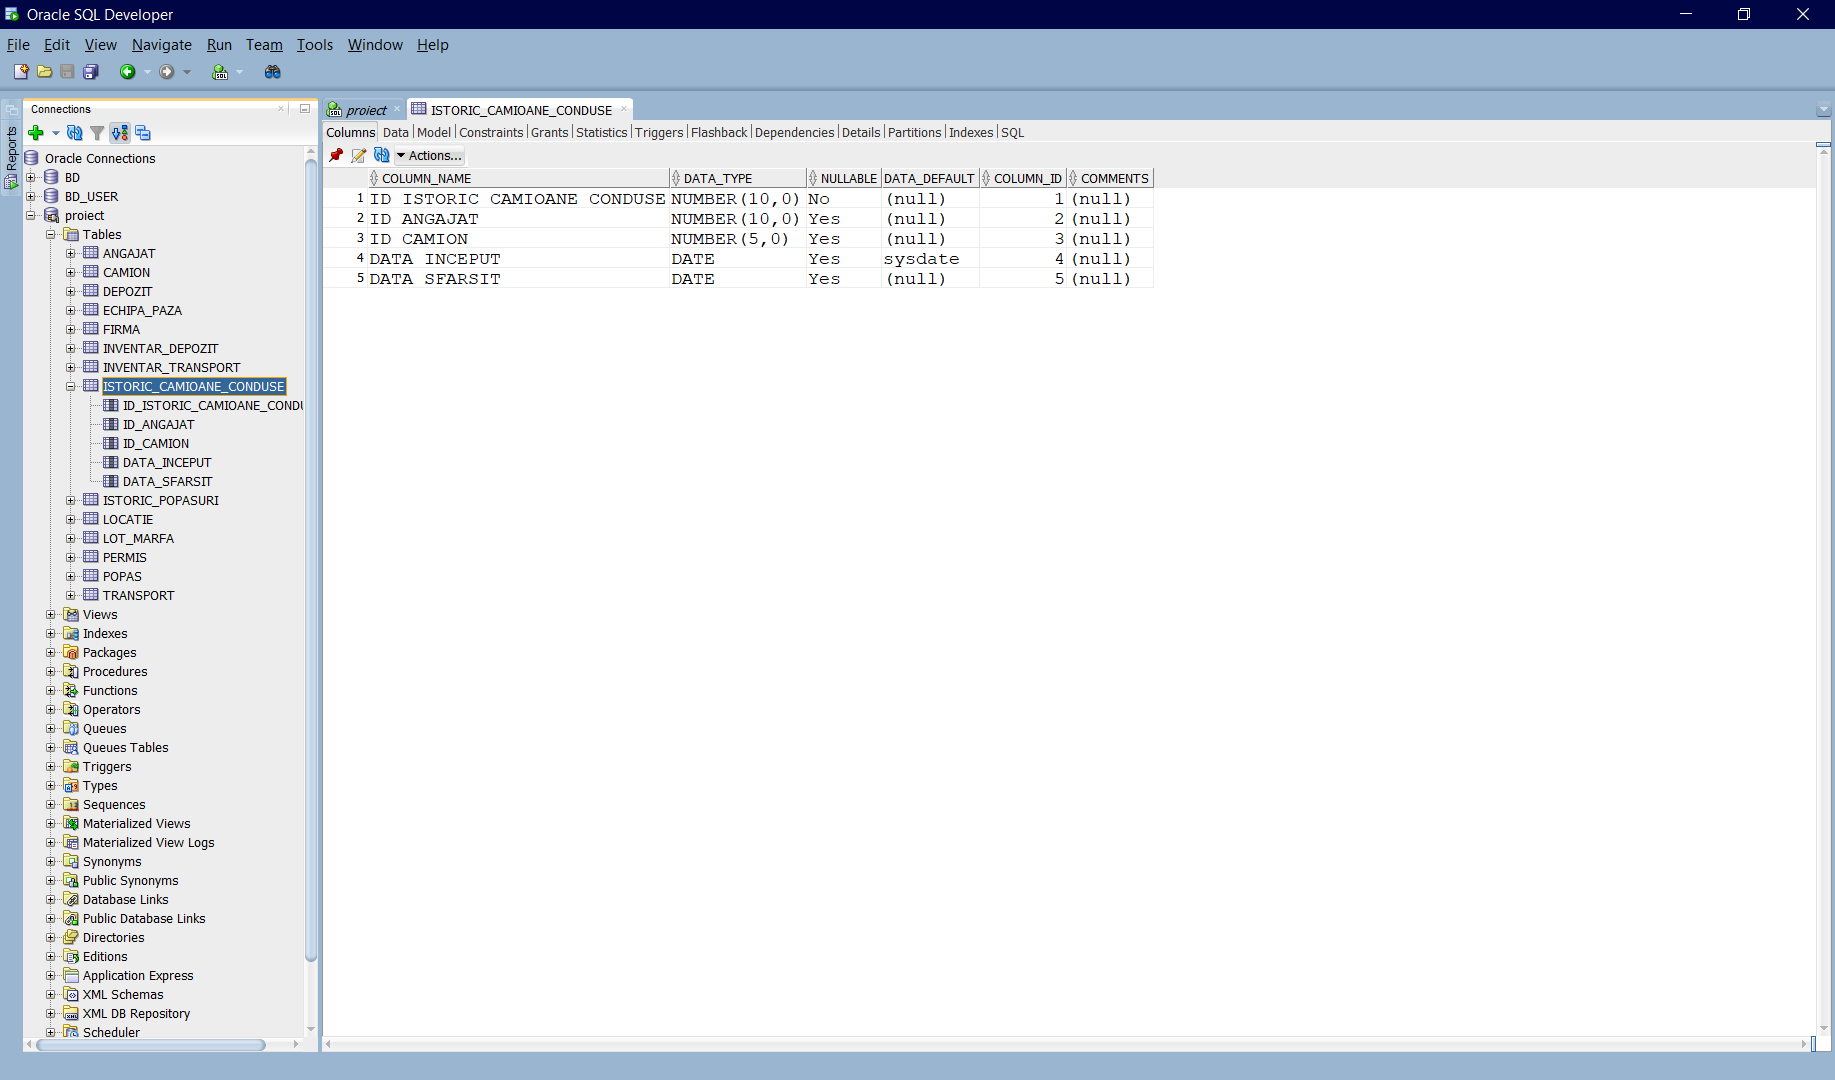
\includegraphics[width=\textwidth]{tabele.png}
\label{tabele_create}
\centering Tabele create

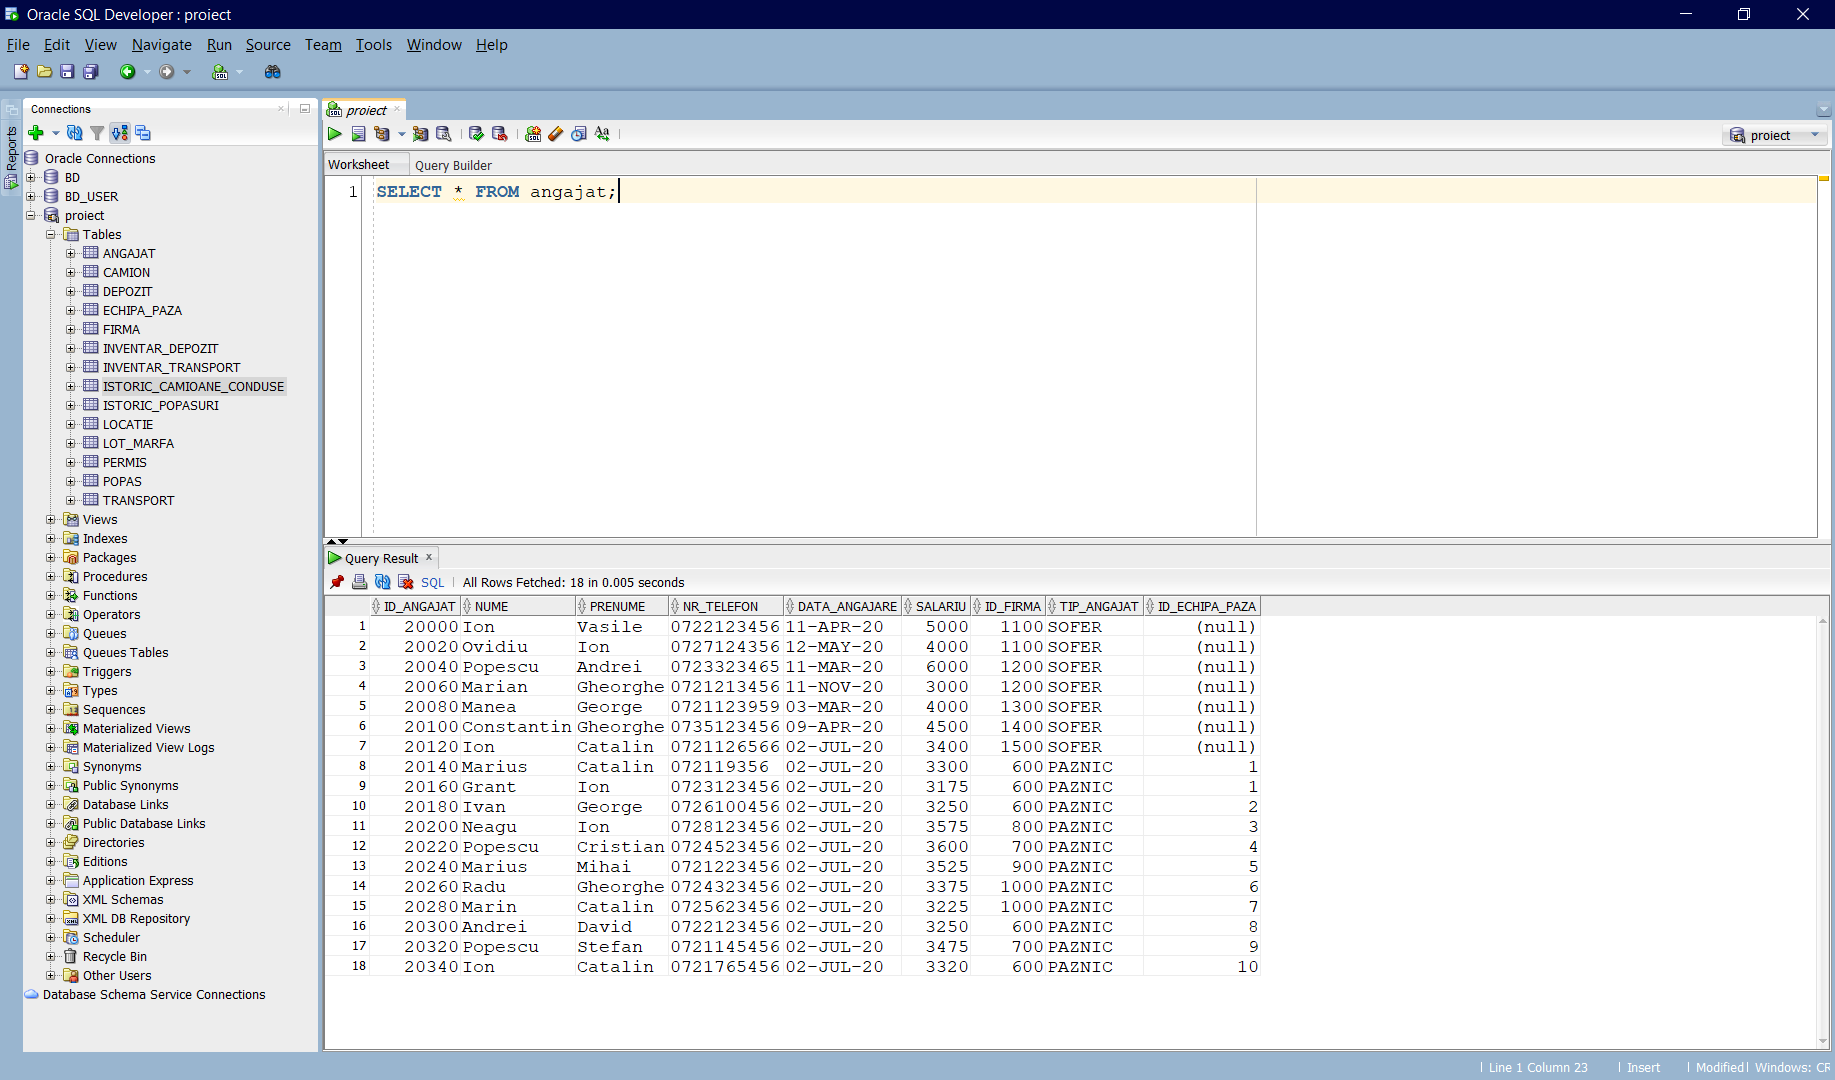
\includegraphics[width=\textwidth]{date_tabel_ang.png}
\label{date_tabel_ang}
\centering Date salvate in tabelul ANGAJAT

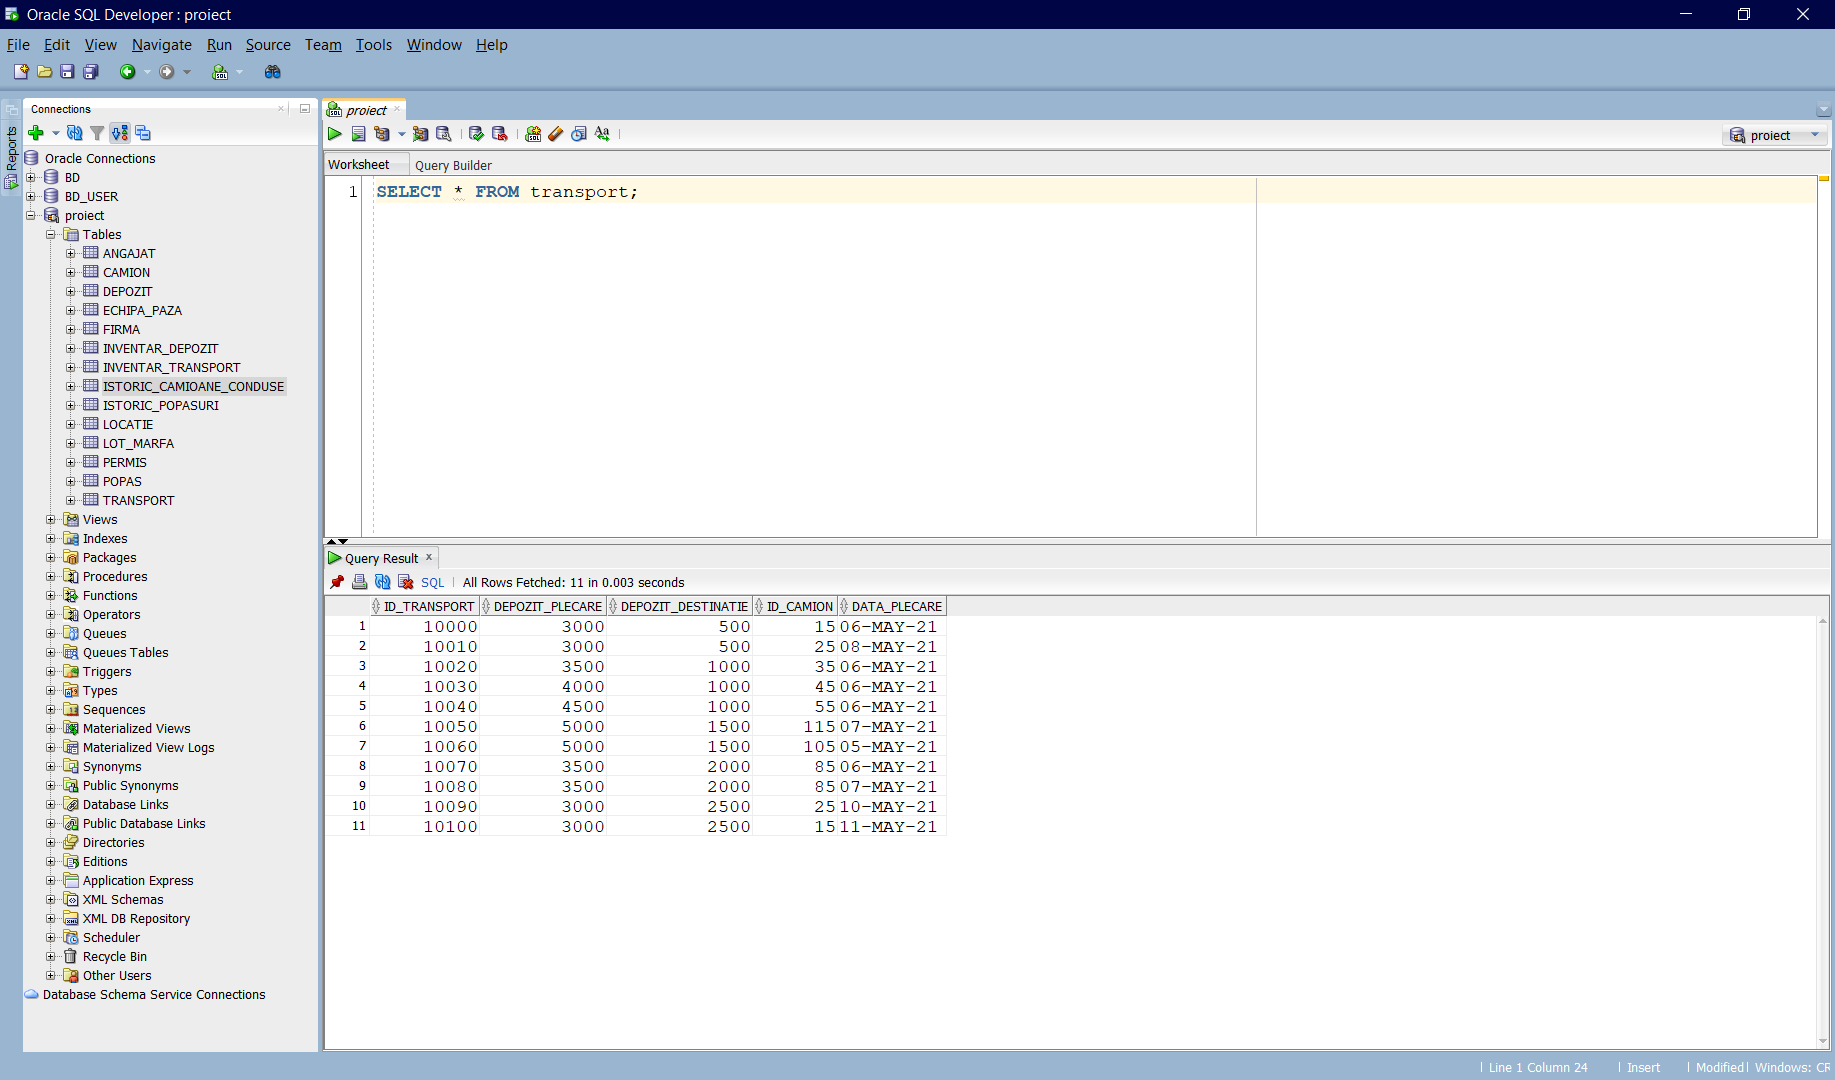
\includegraphics[width=\textwidth]{date_tabel_trans.png}
\label{date_tabel_trans}
\centering Date salvate in tabelul TRANSPORT

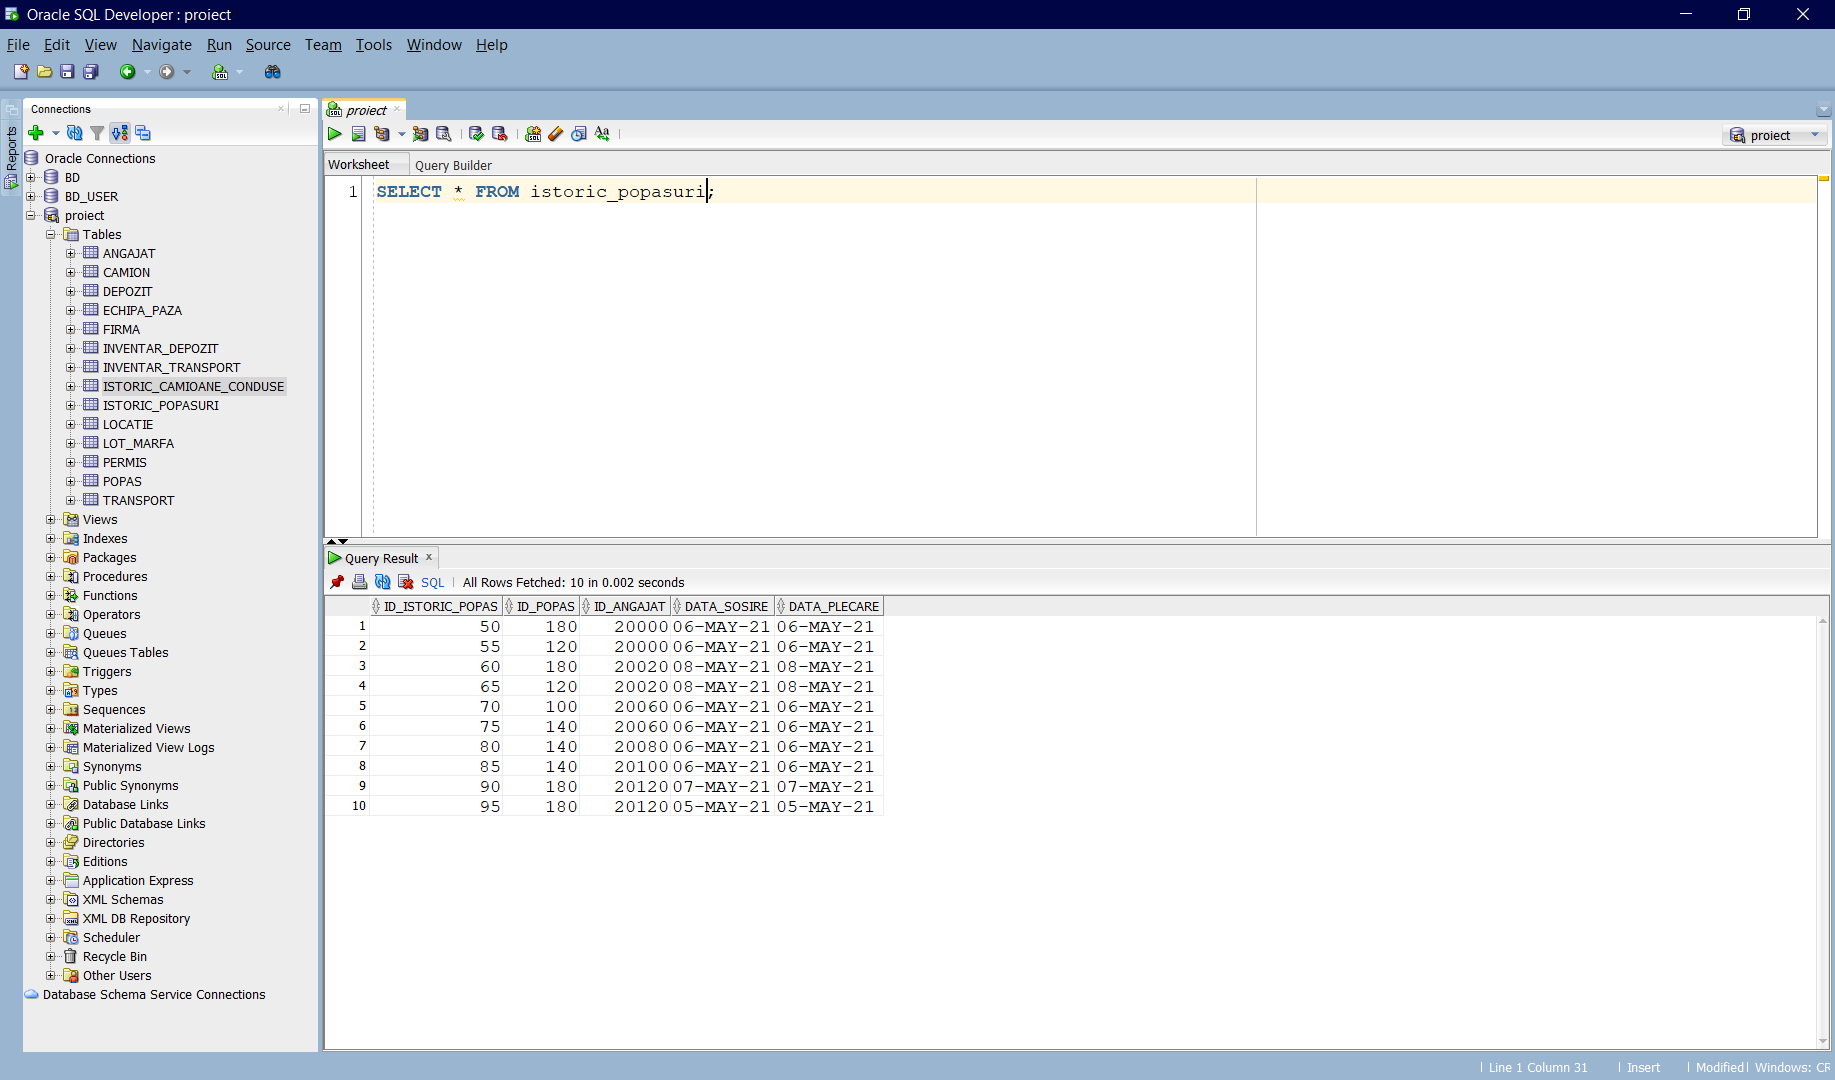
\includegraphics[width=\textwidth]{date_tabel_ist_pop.png}

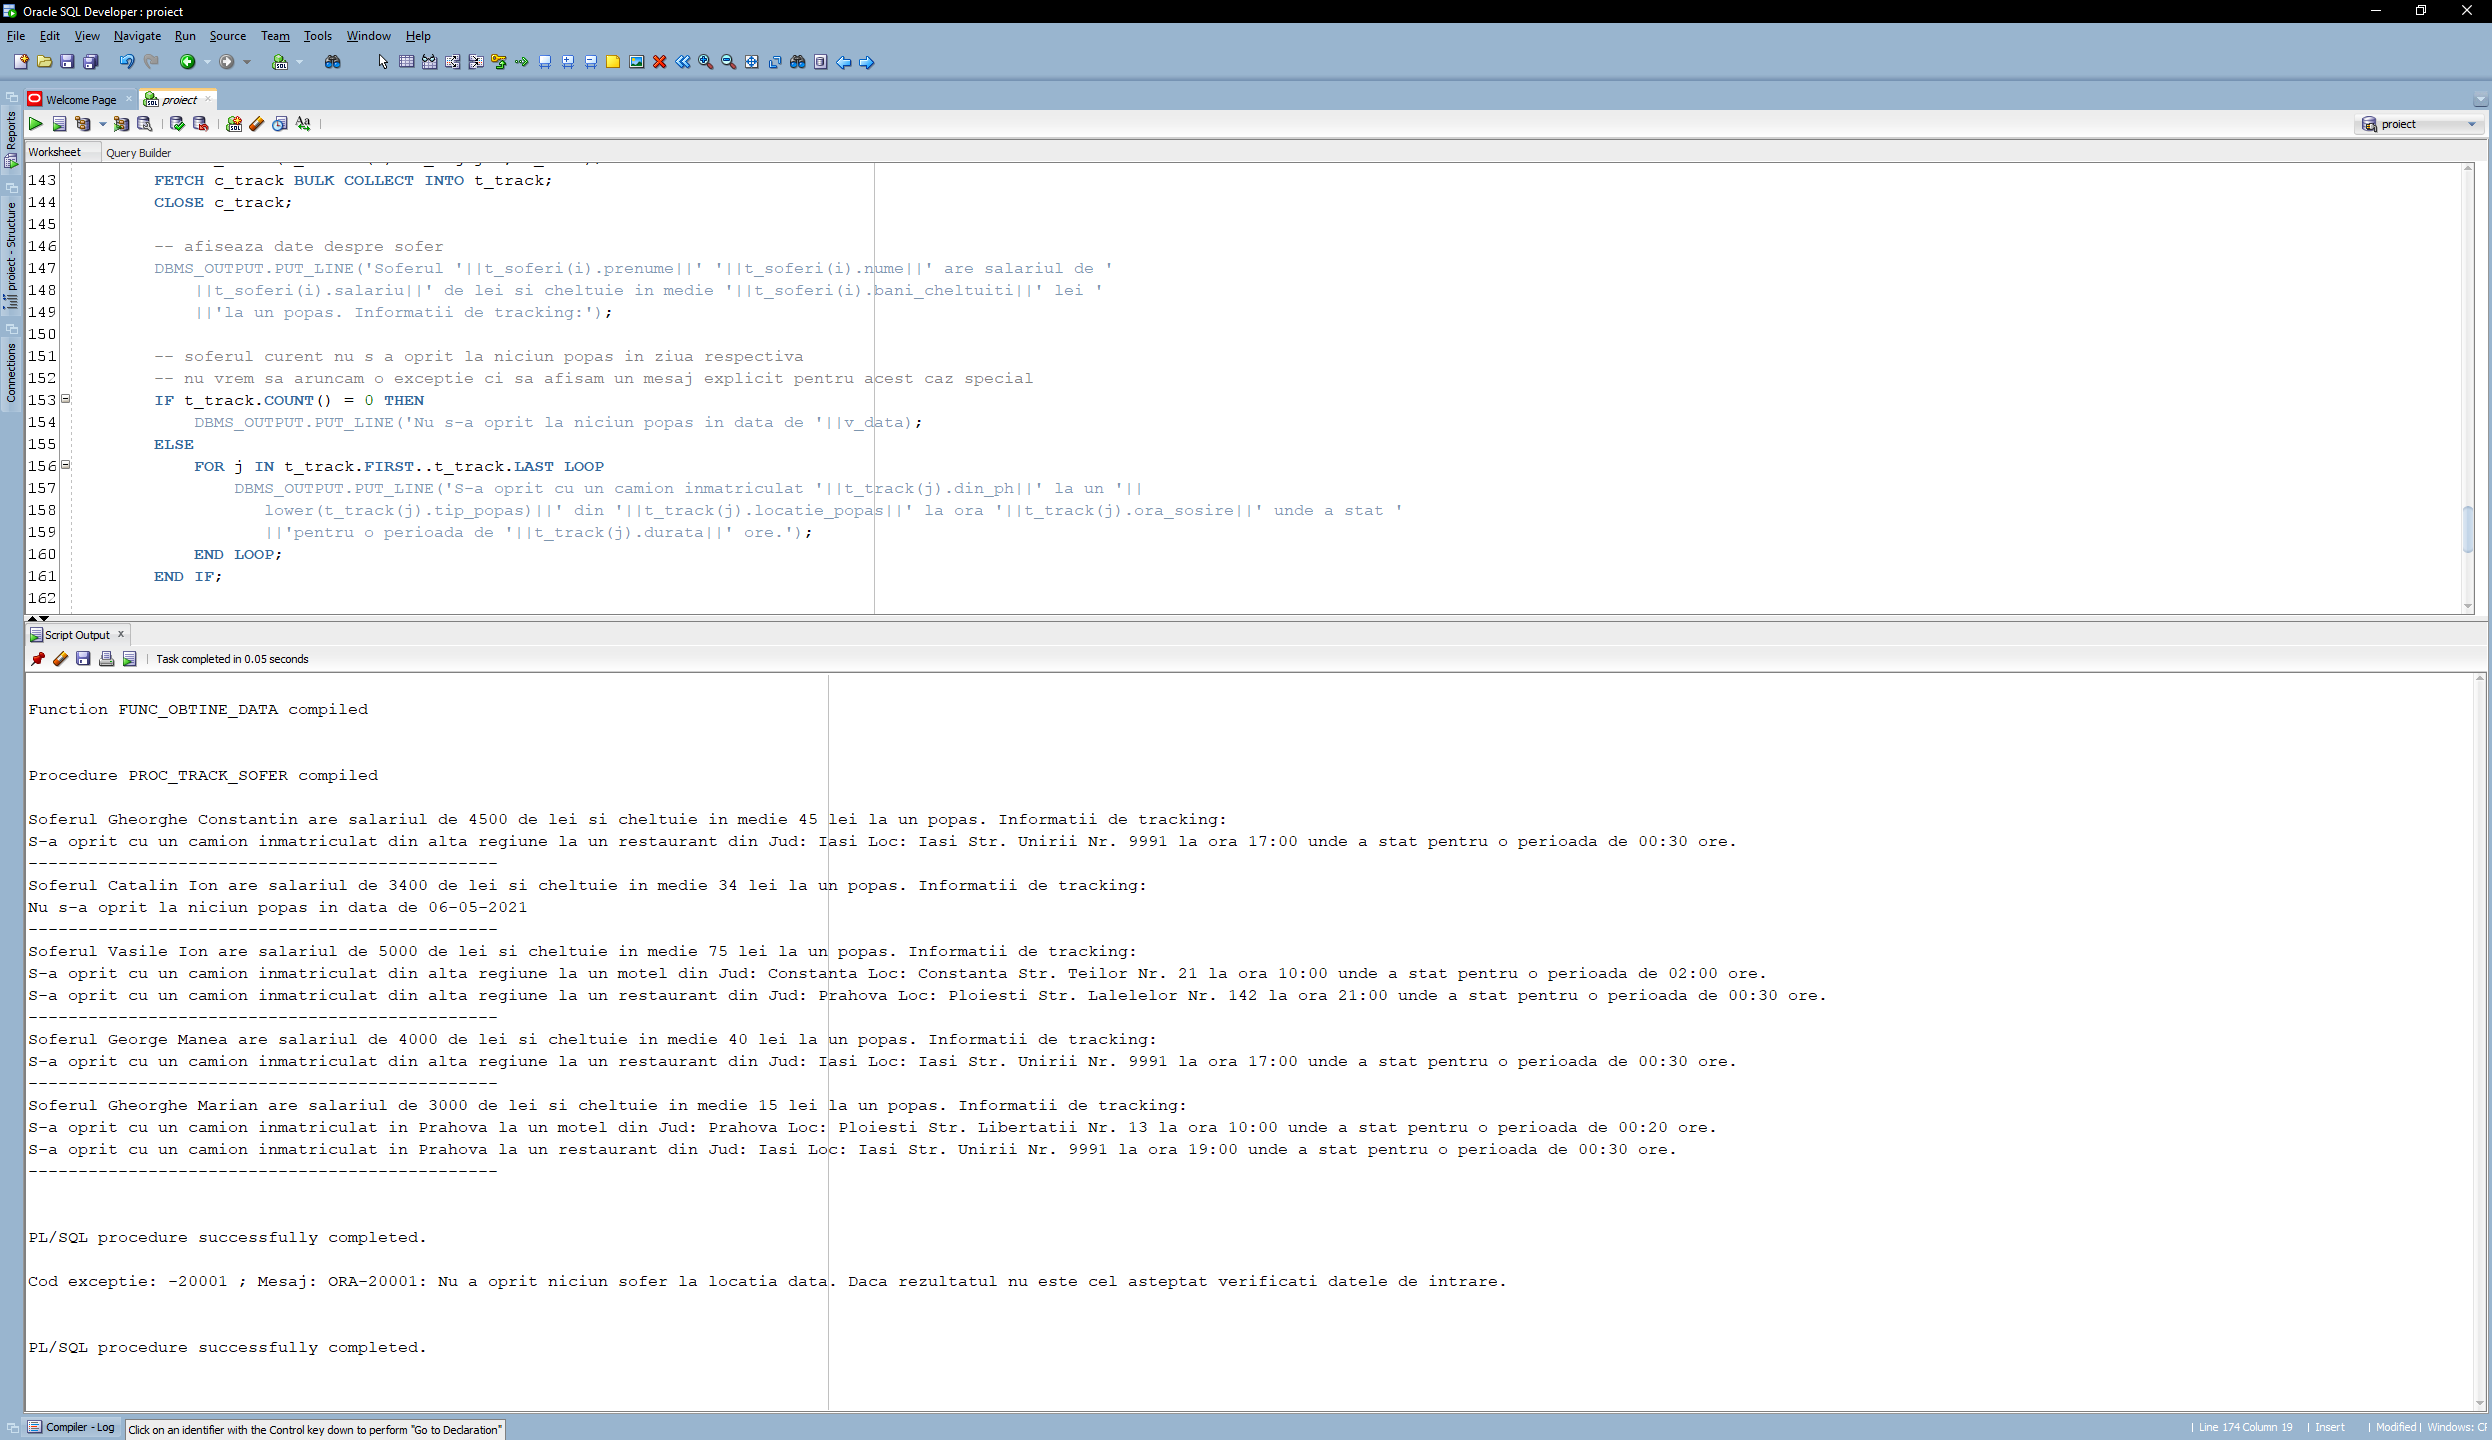
\includegraphics[width=\textwidth]{6_1.png}

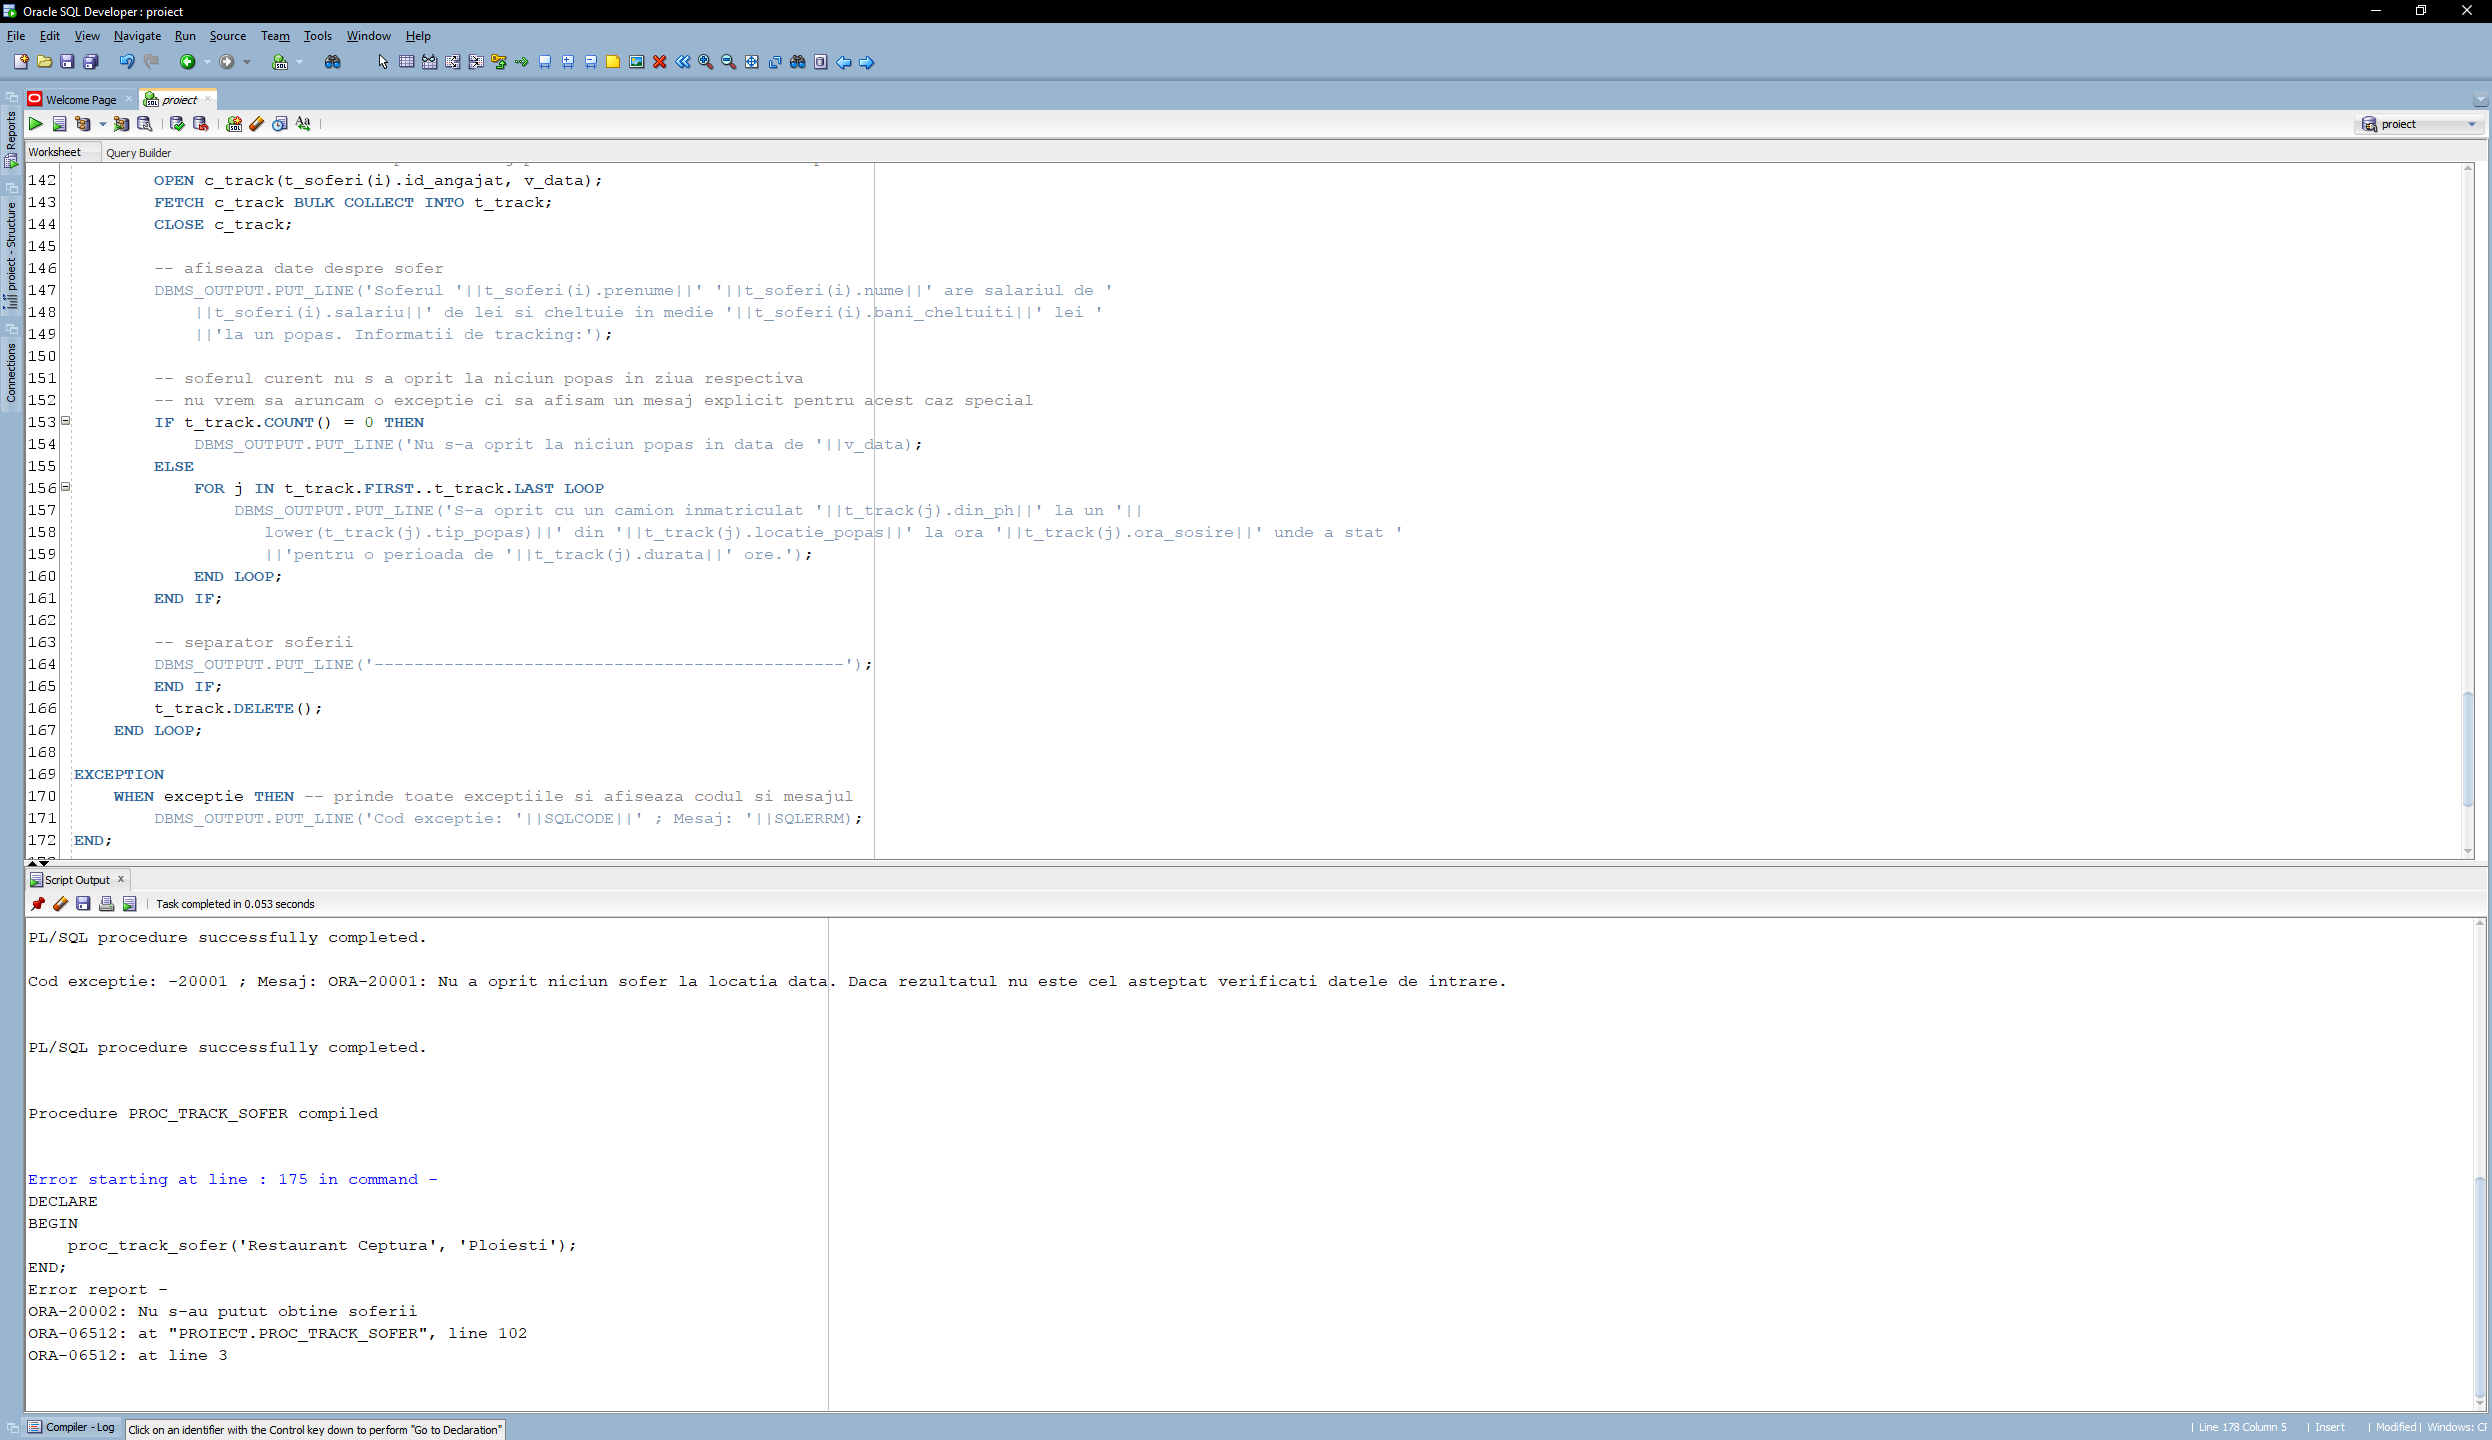
\includegraphics[width=\textwidth]{6_2.png}

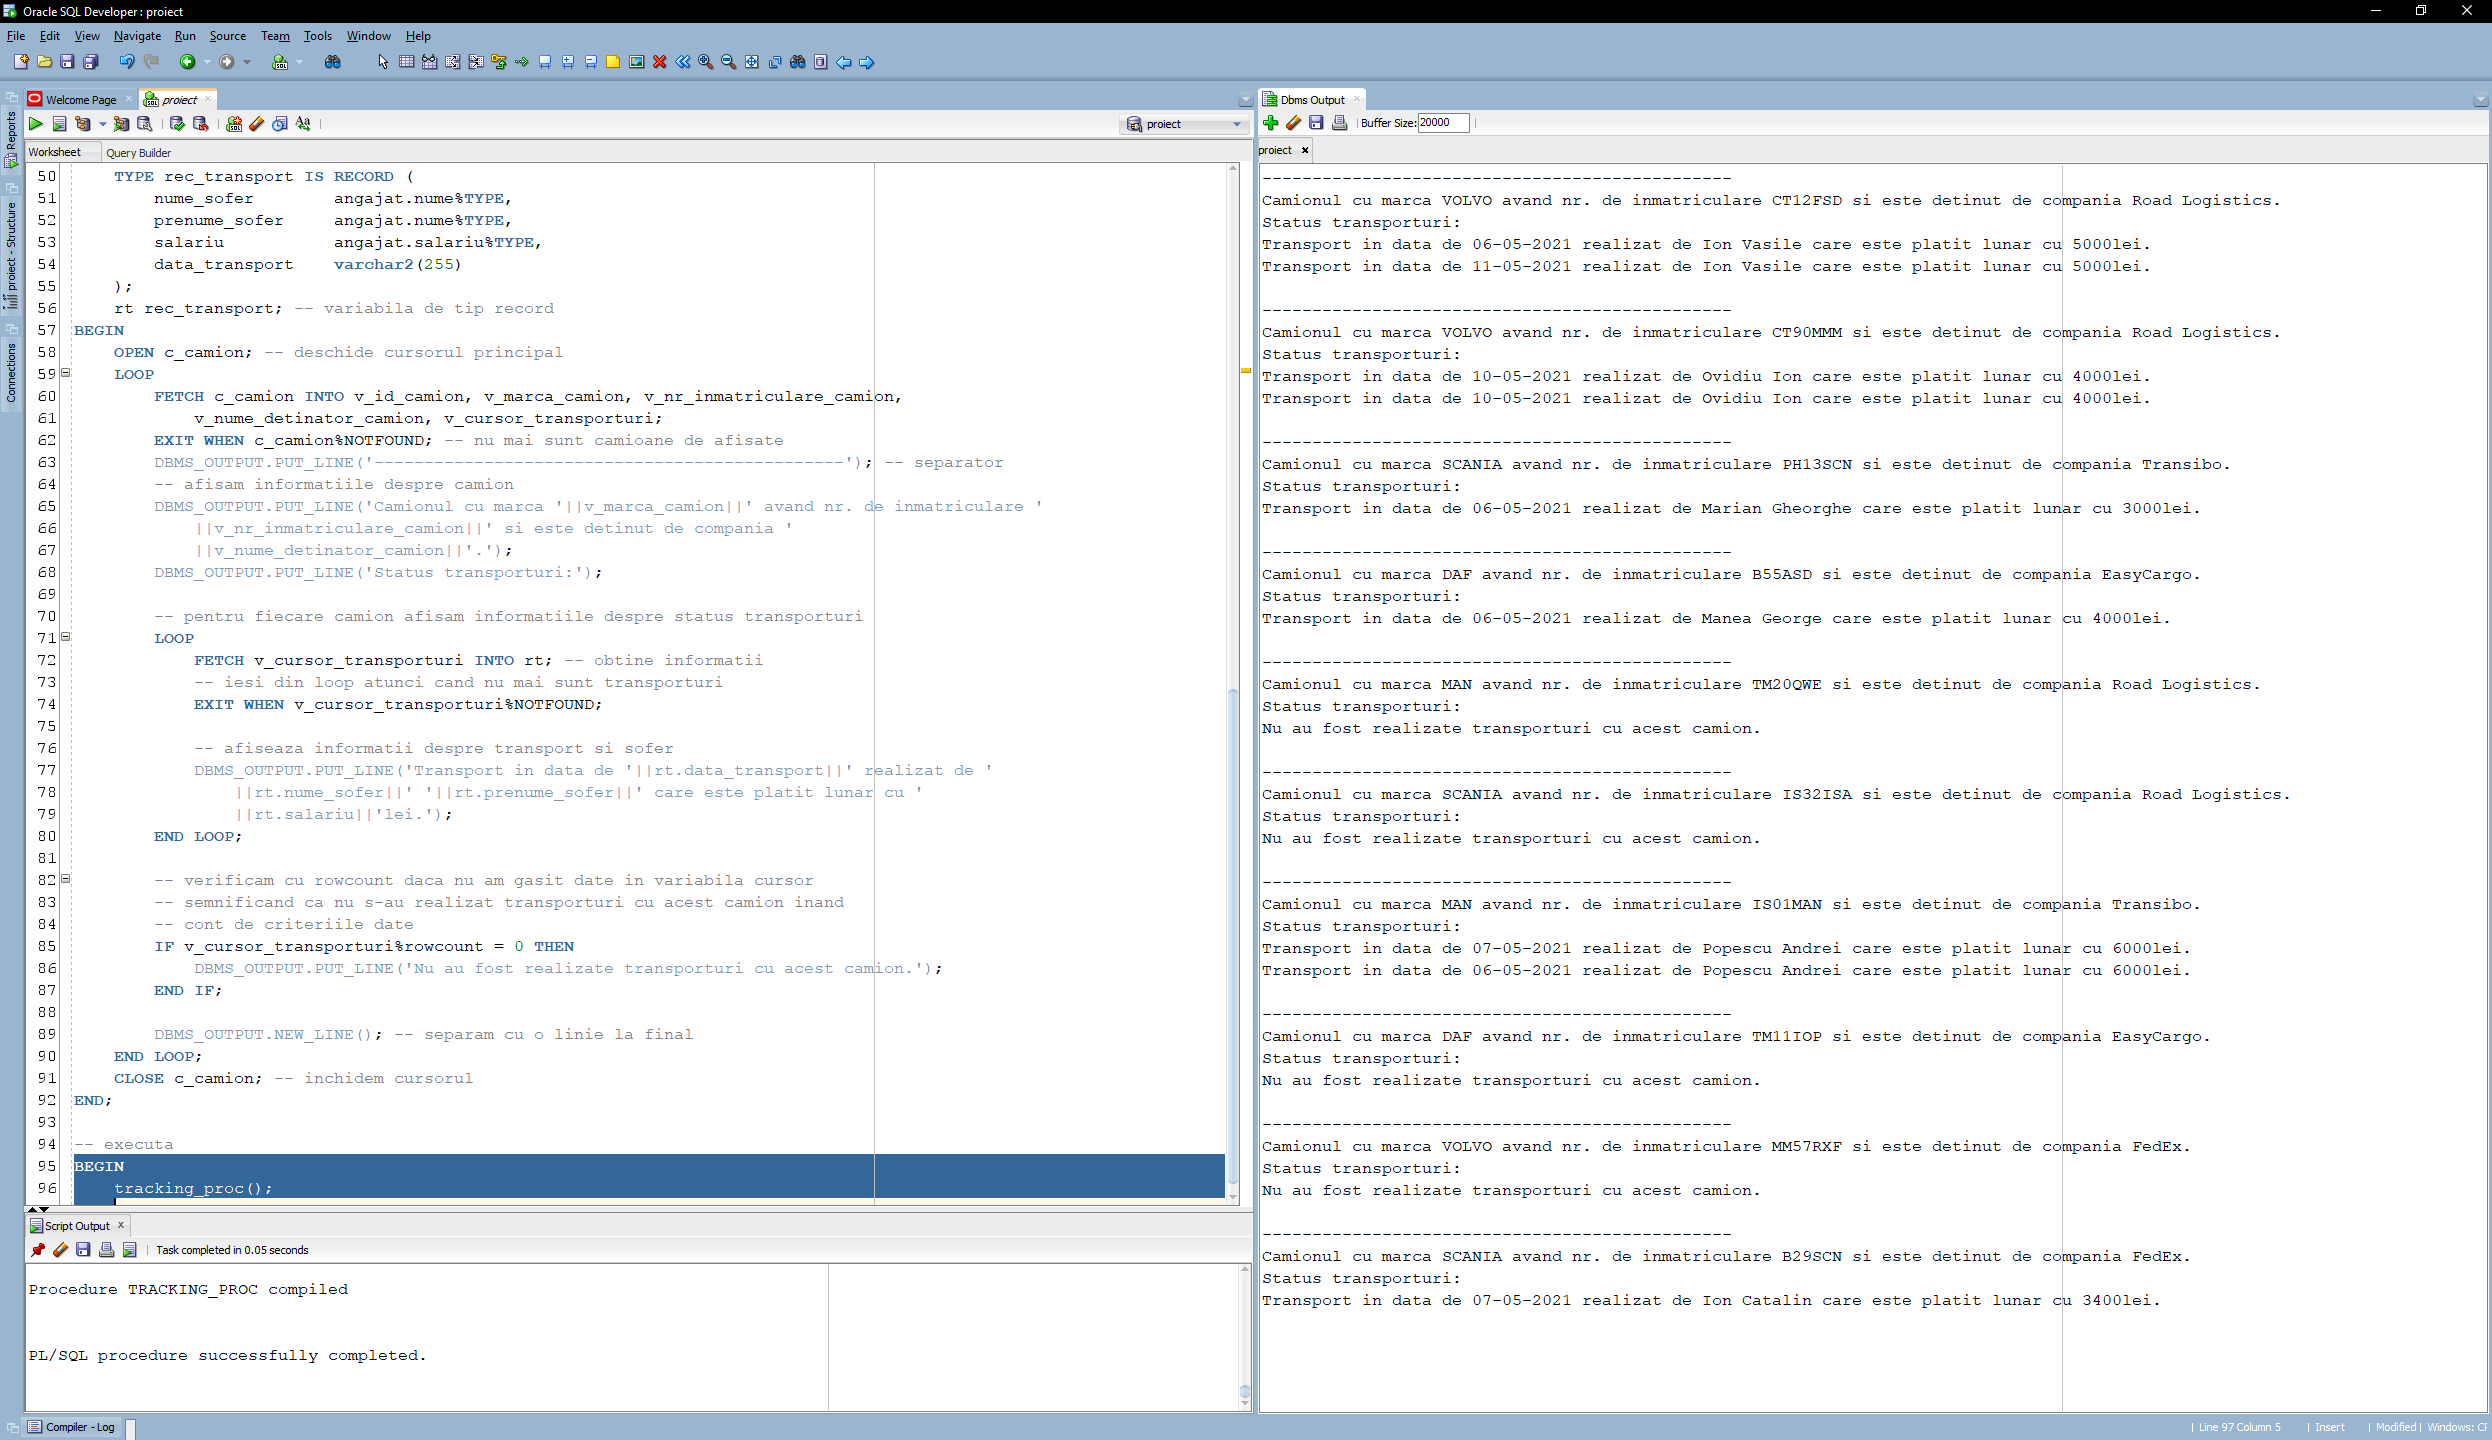
\includegraphics[width=\textwidth]{7_1.png}

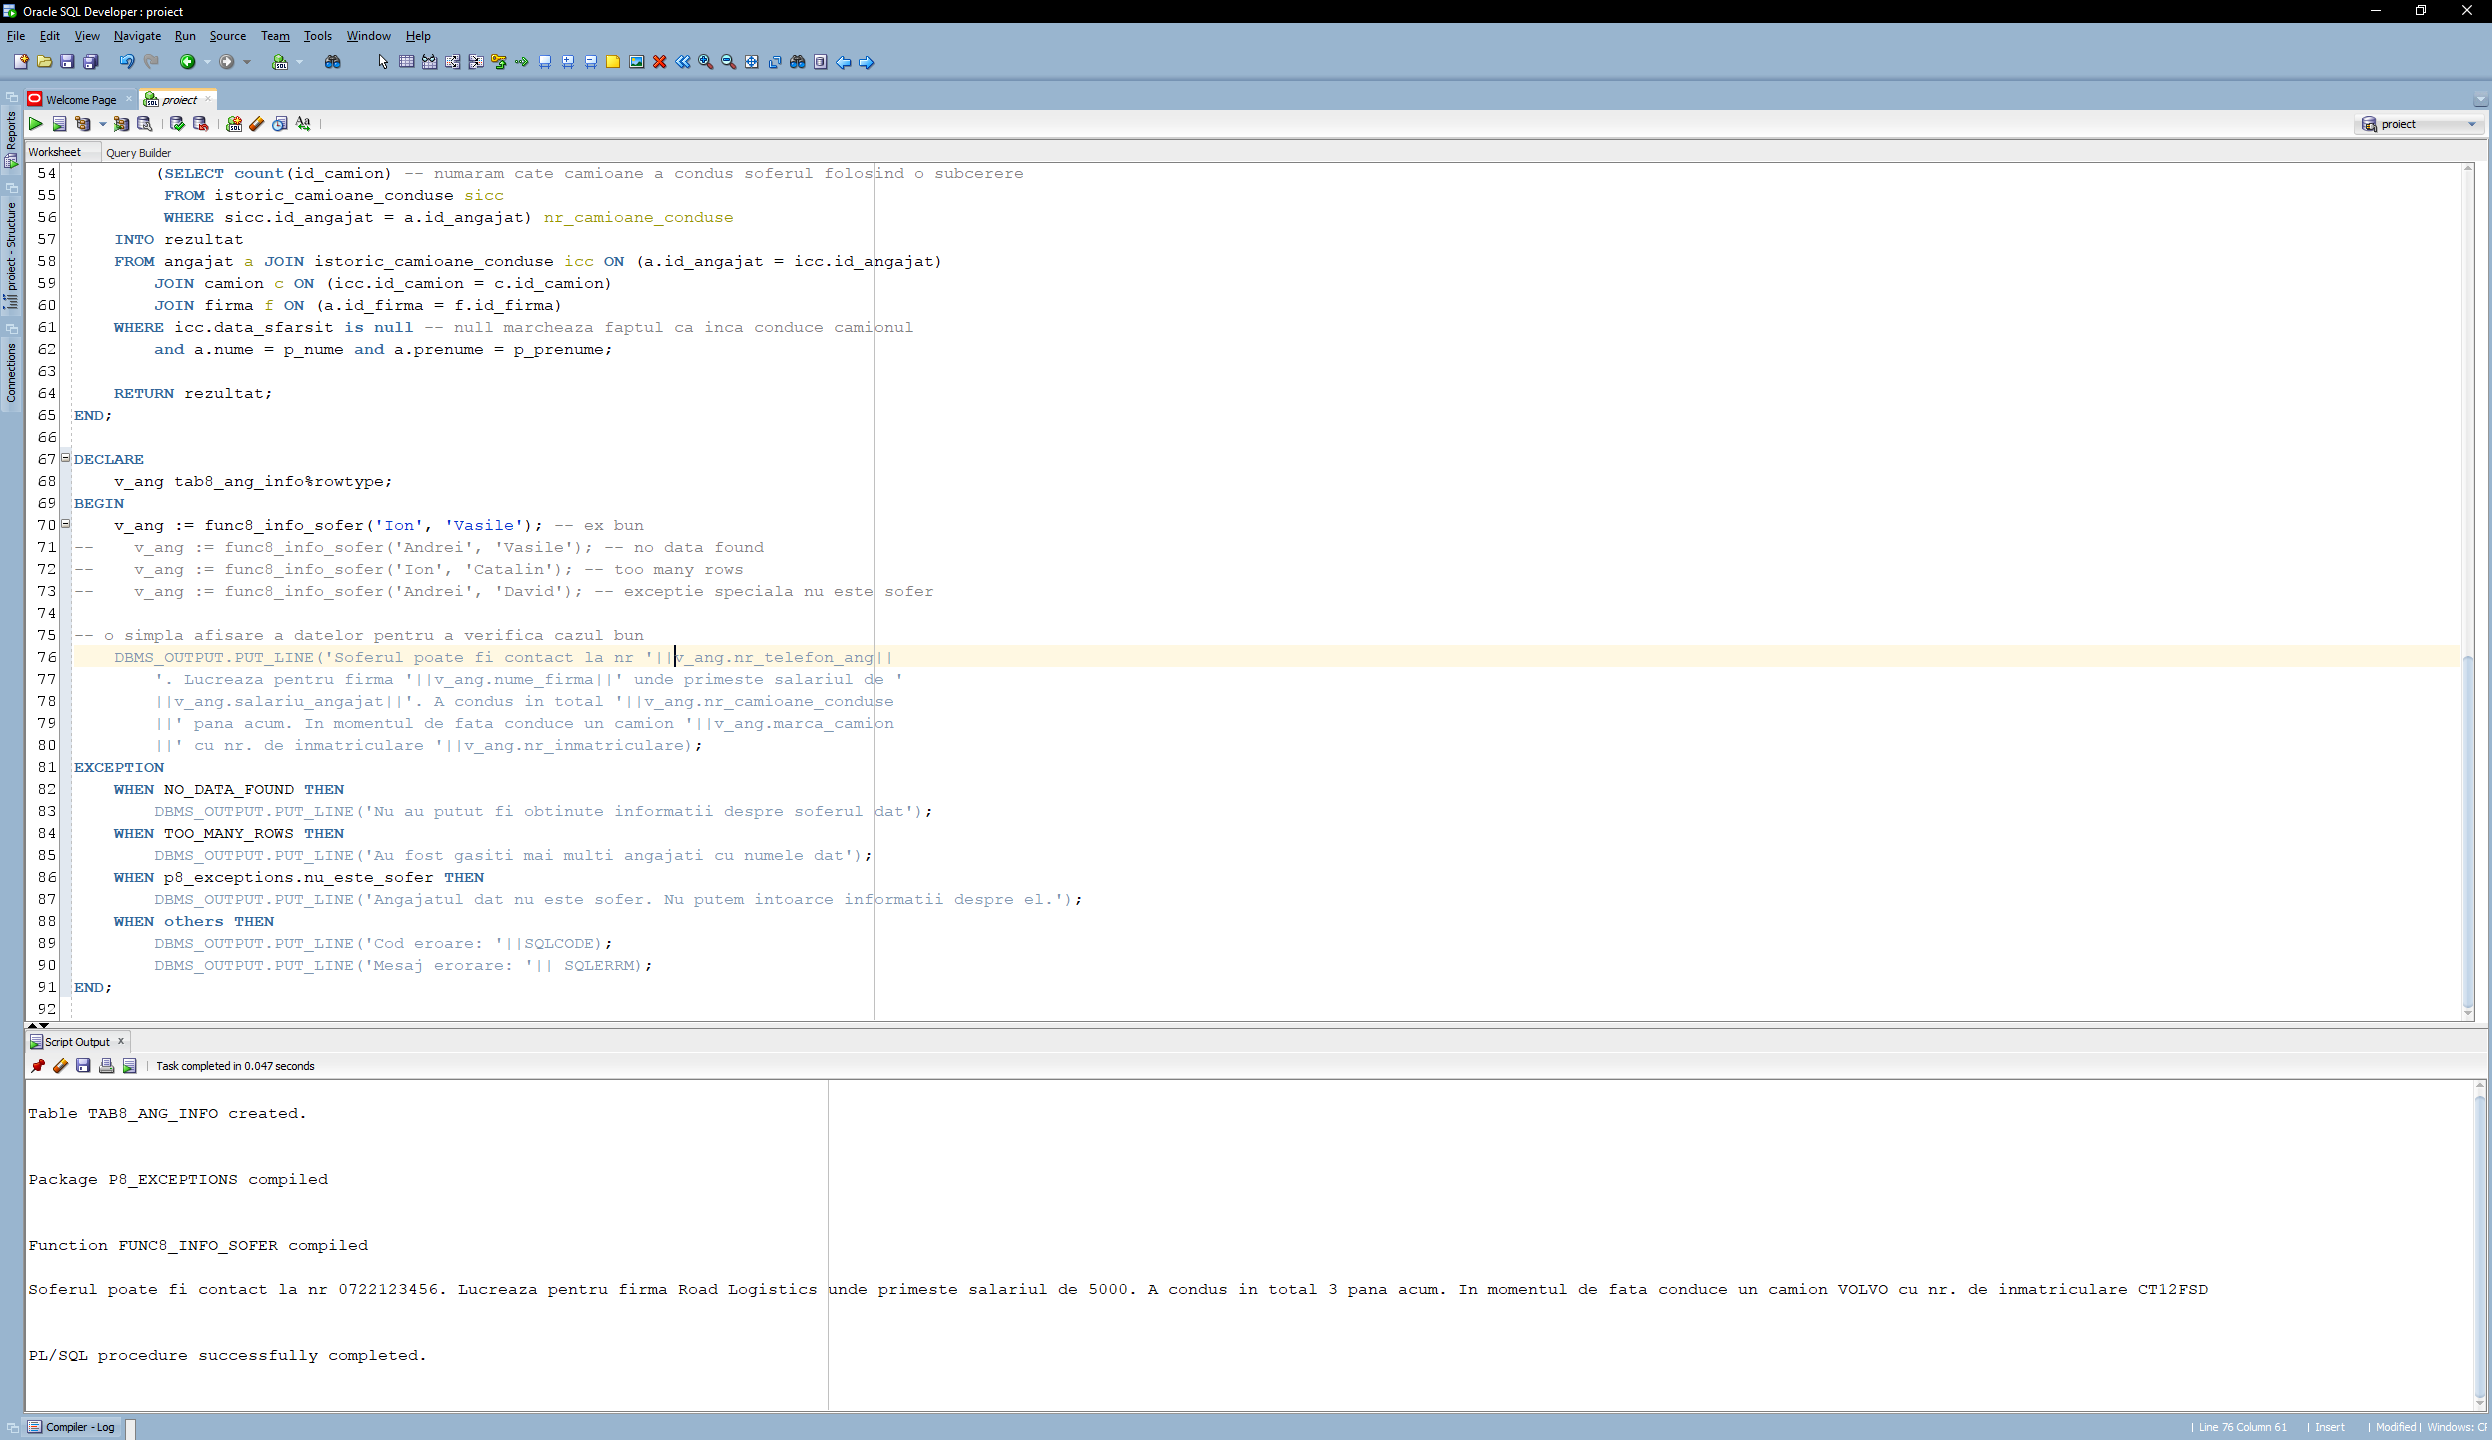
\includegraphics[width=\textwidth]{8_1.png}

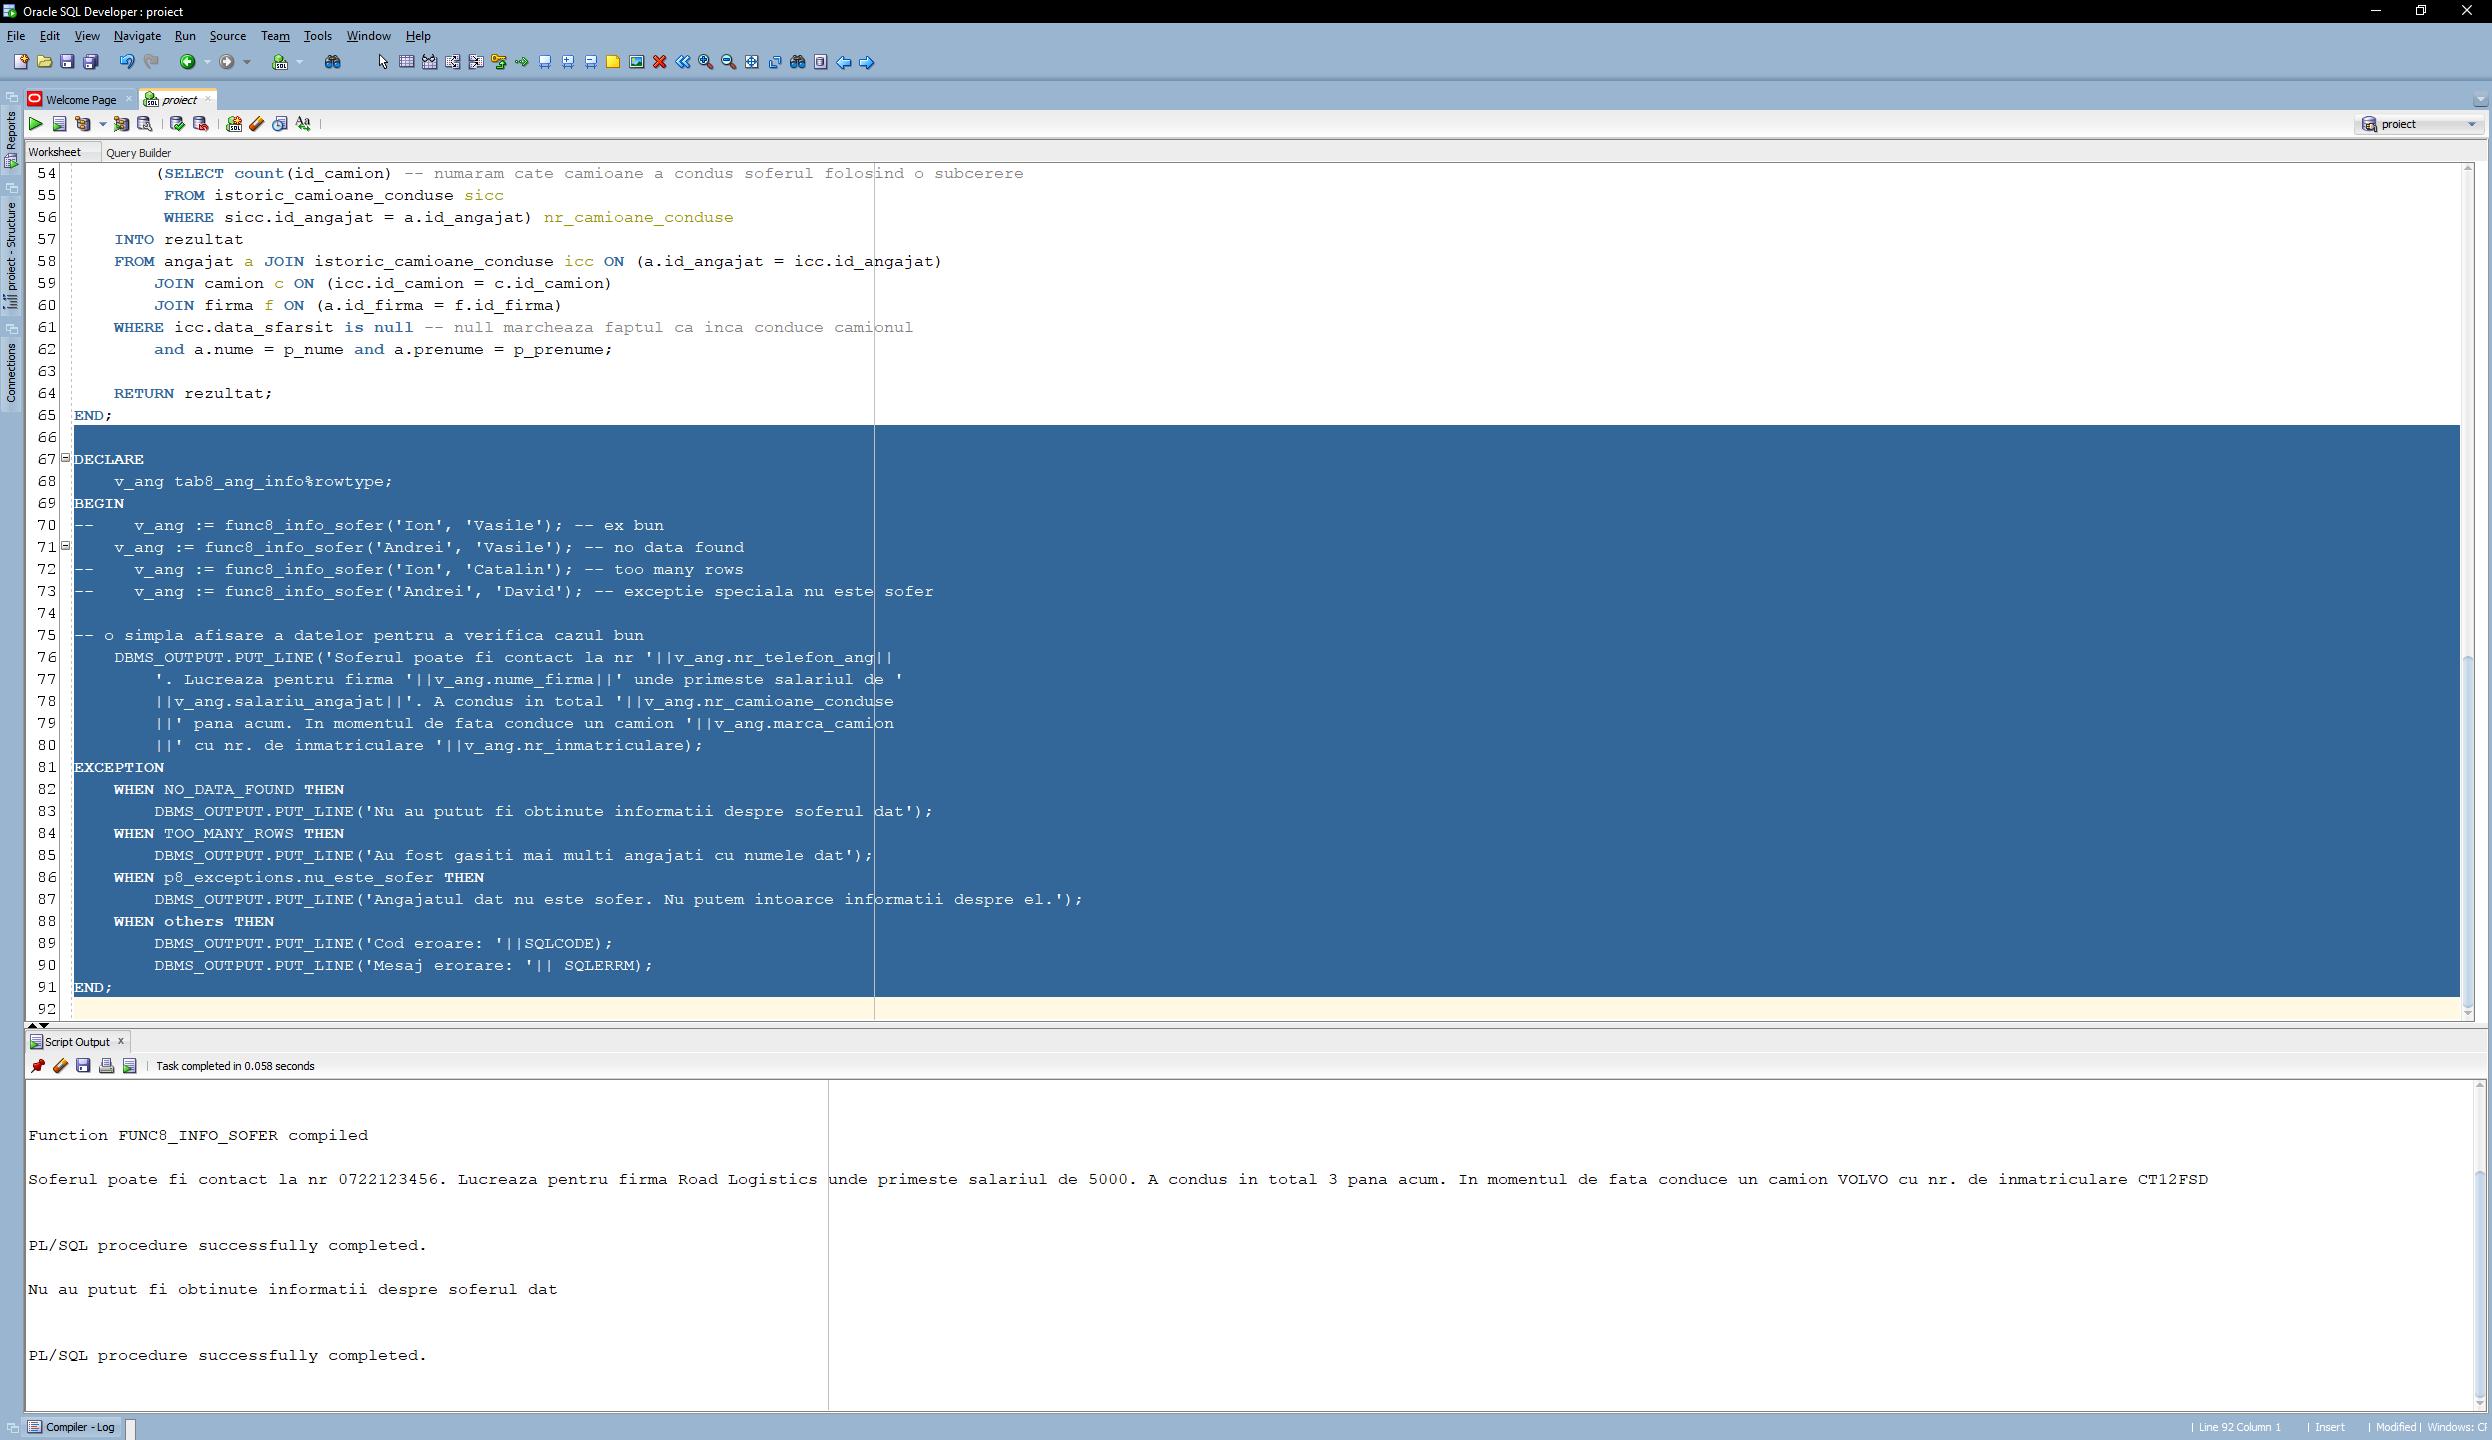
\includegraphics[width=\textwidth]{8_2.png}

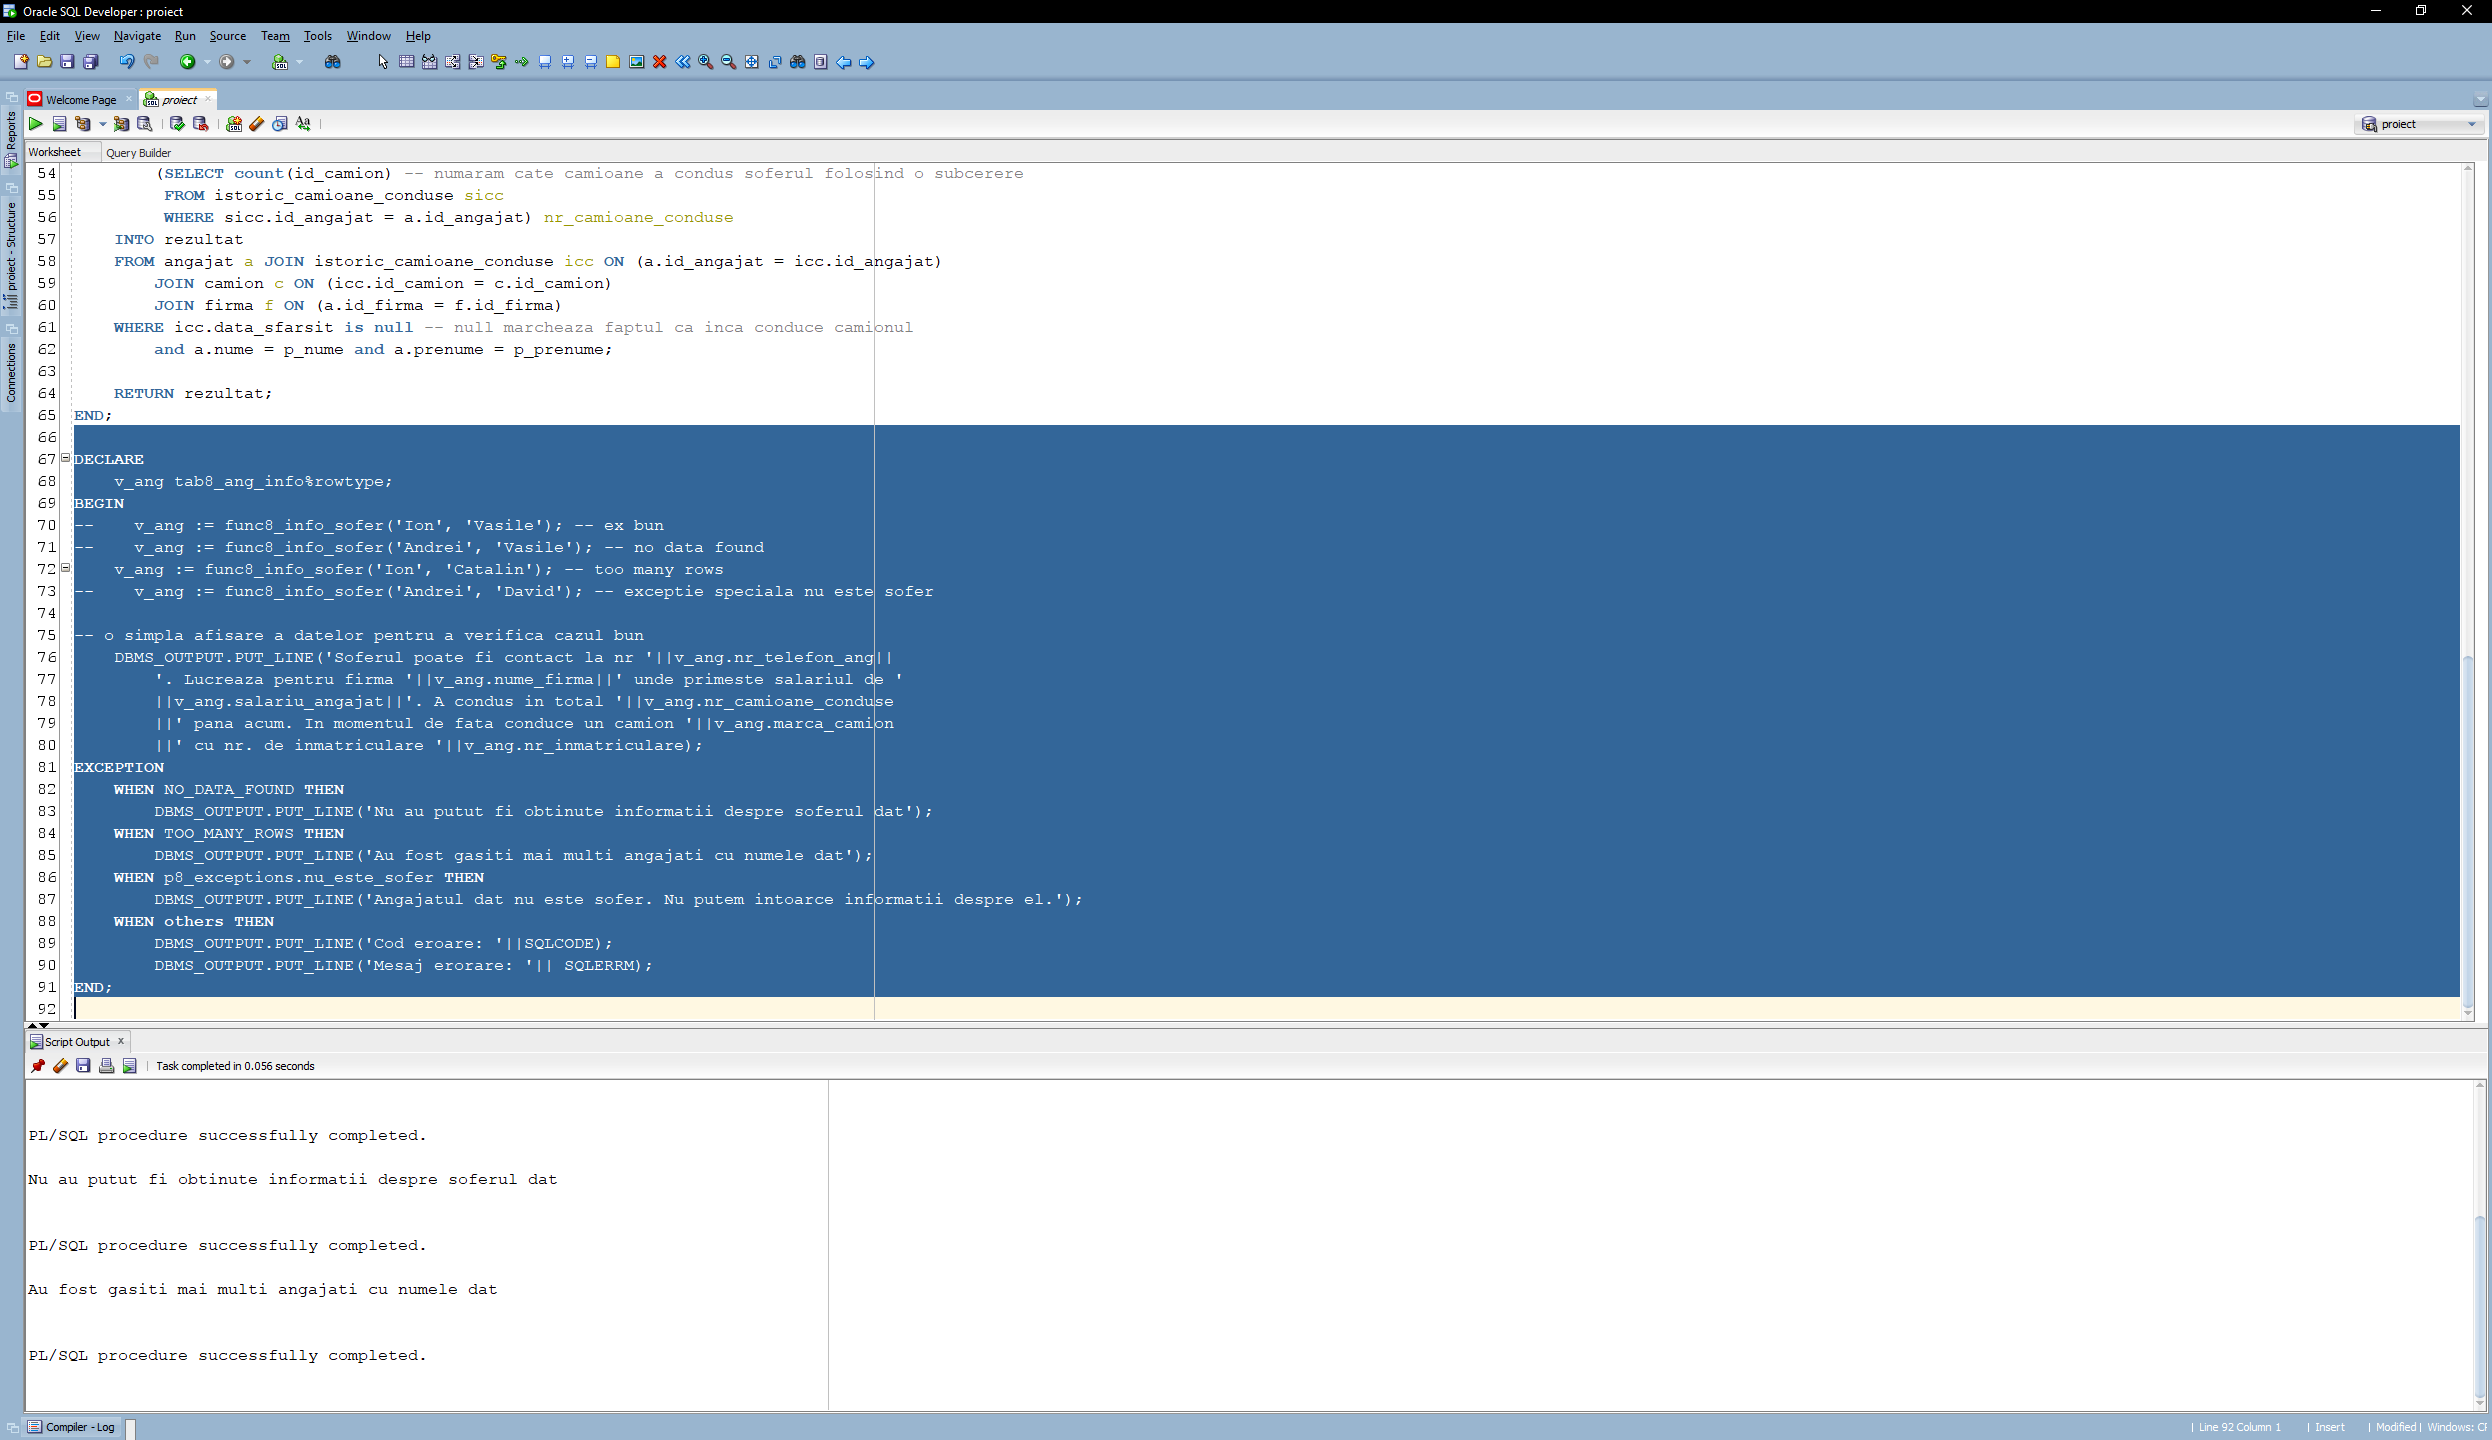
\includegraphics[width=\textwidth]{8_3.png}

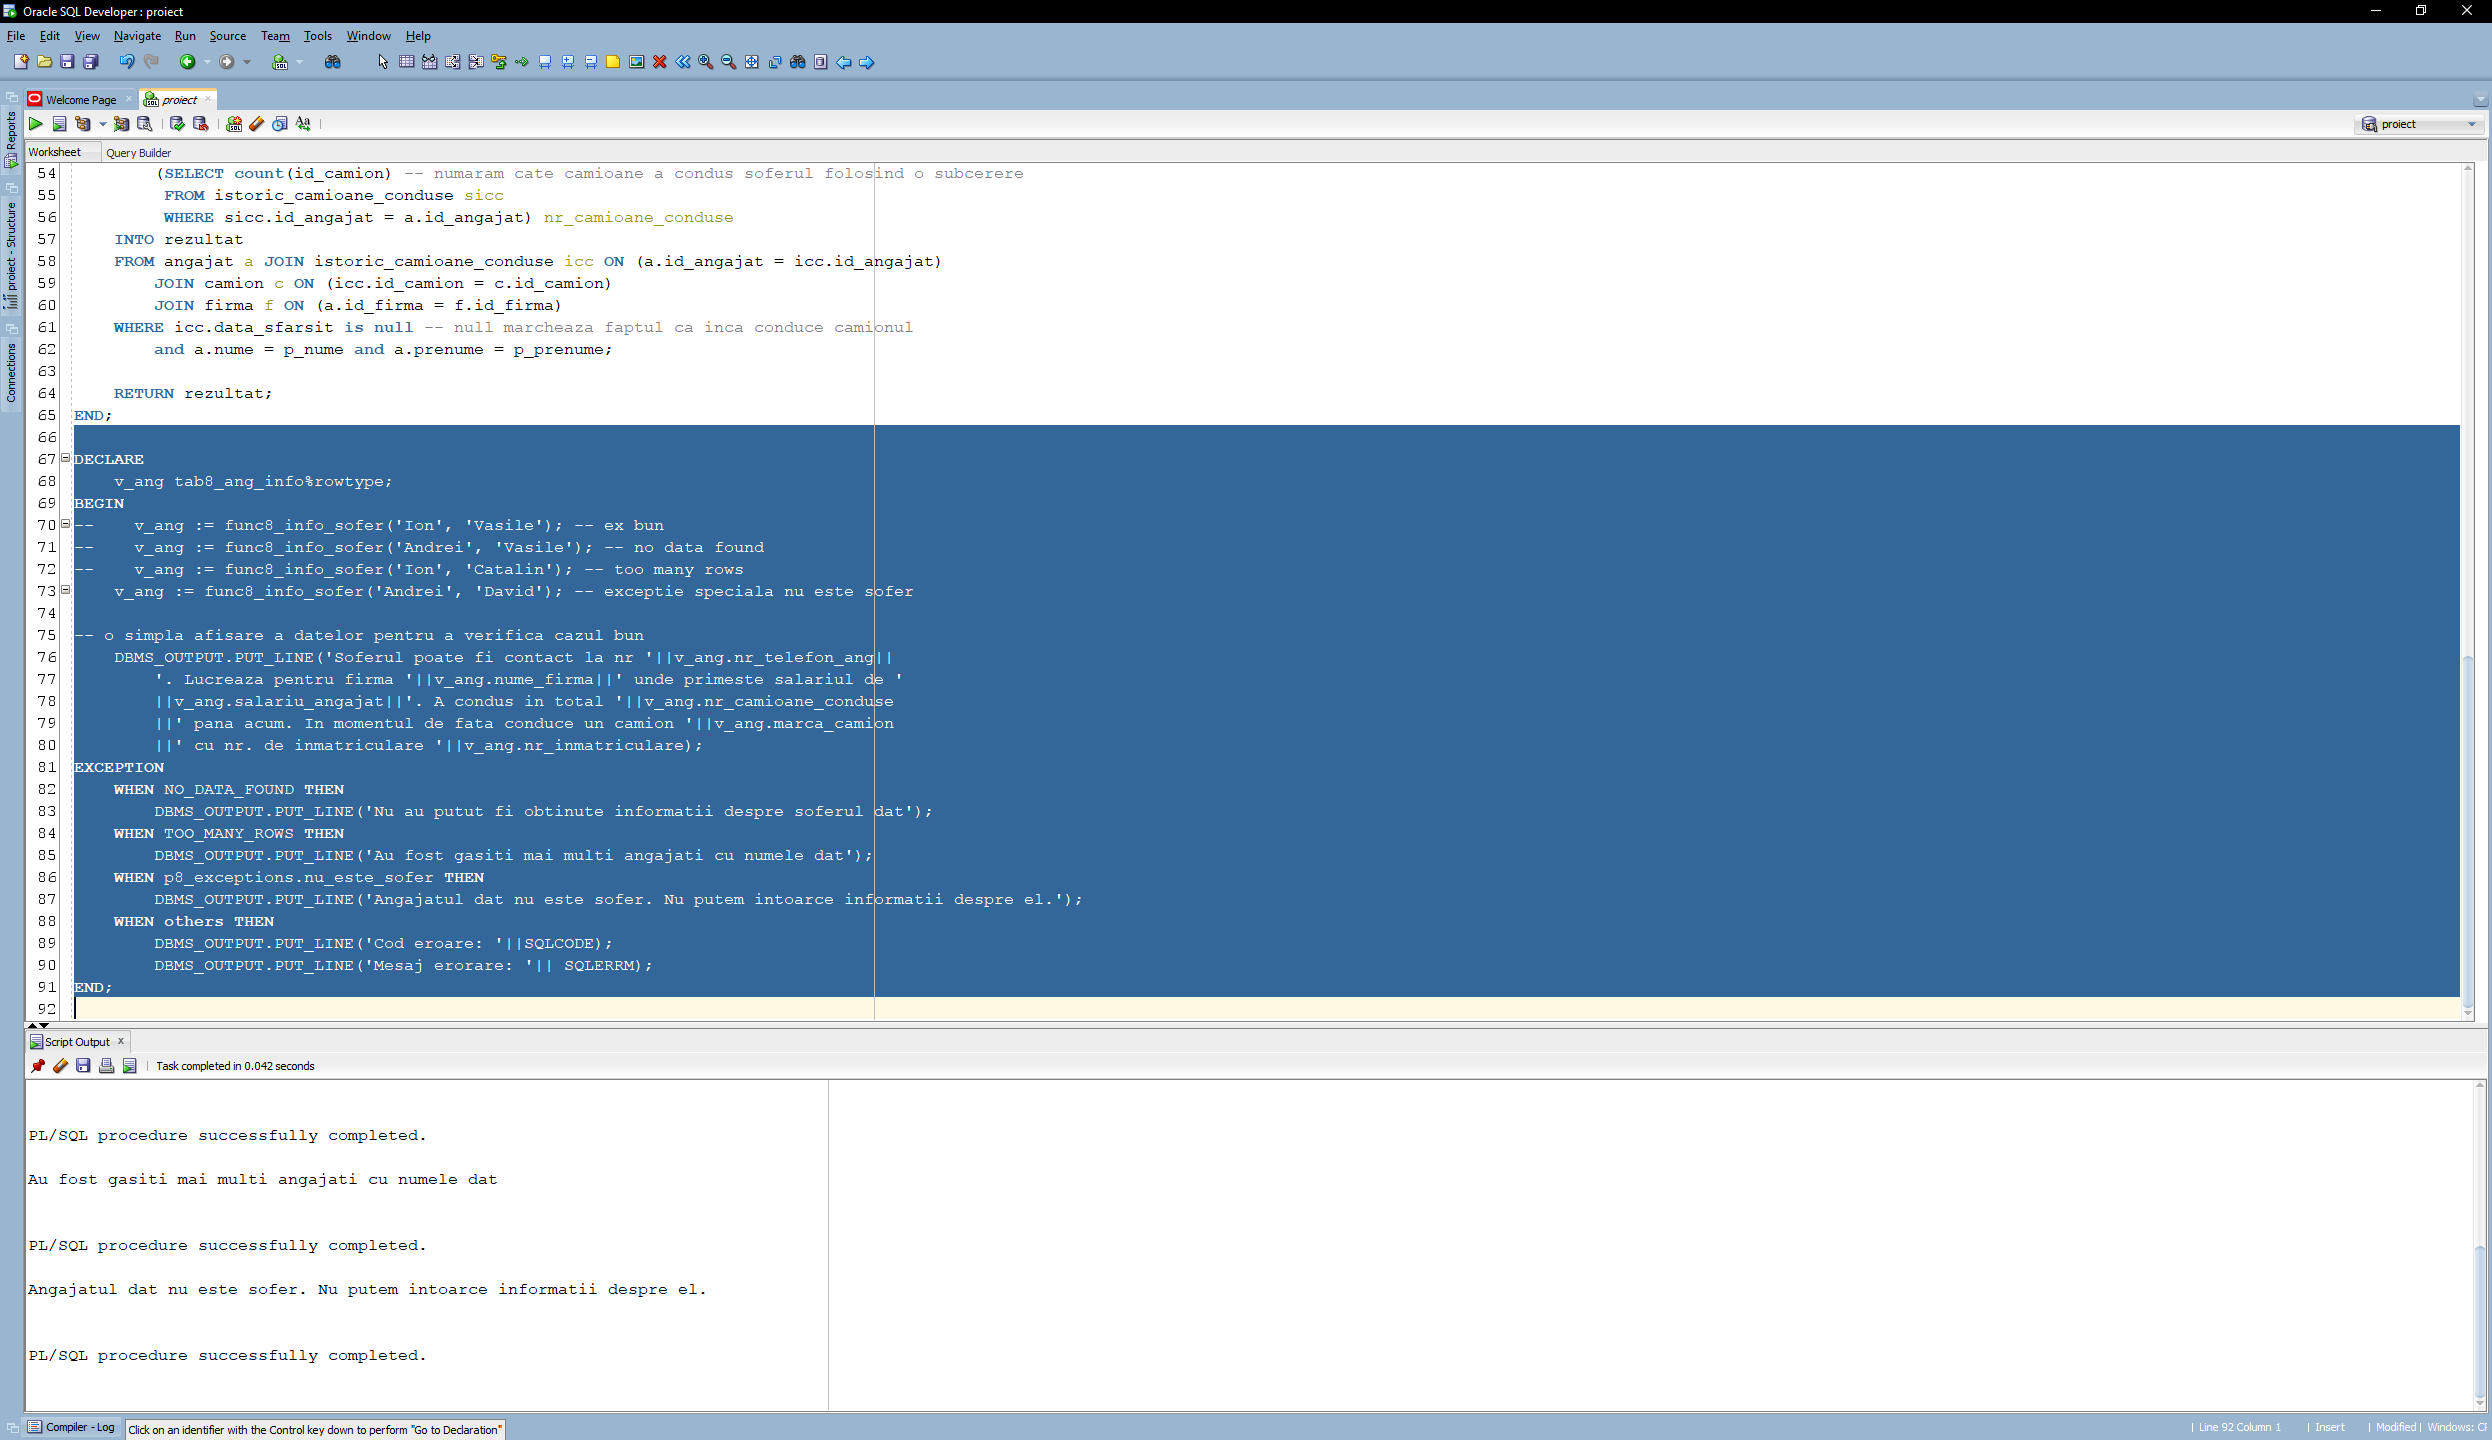
\includegraphics[width=\textwidth]{8_4.png}

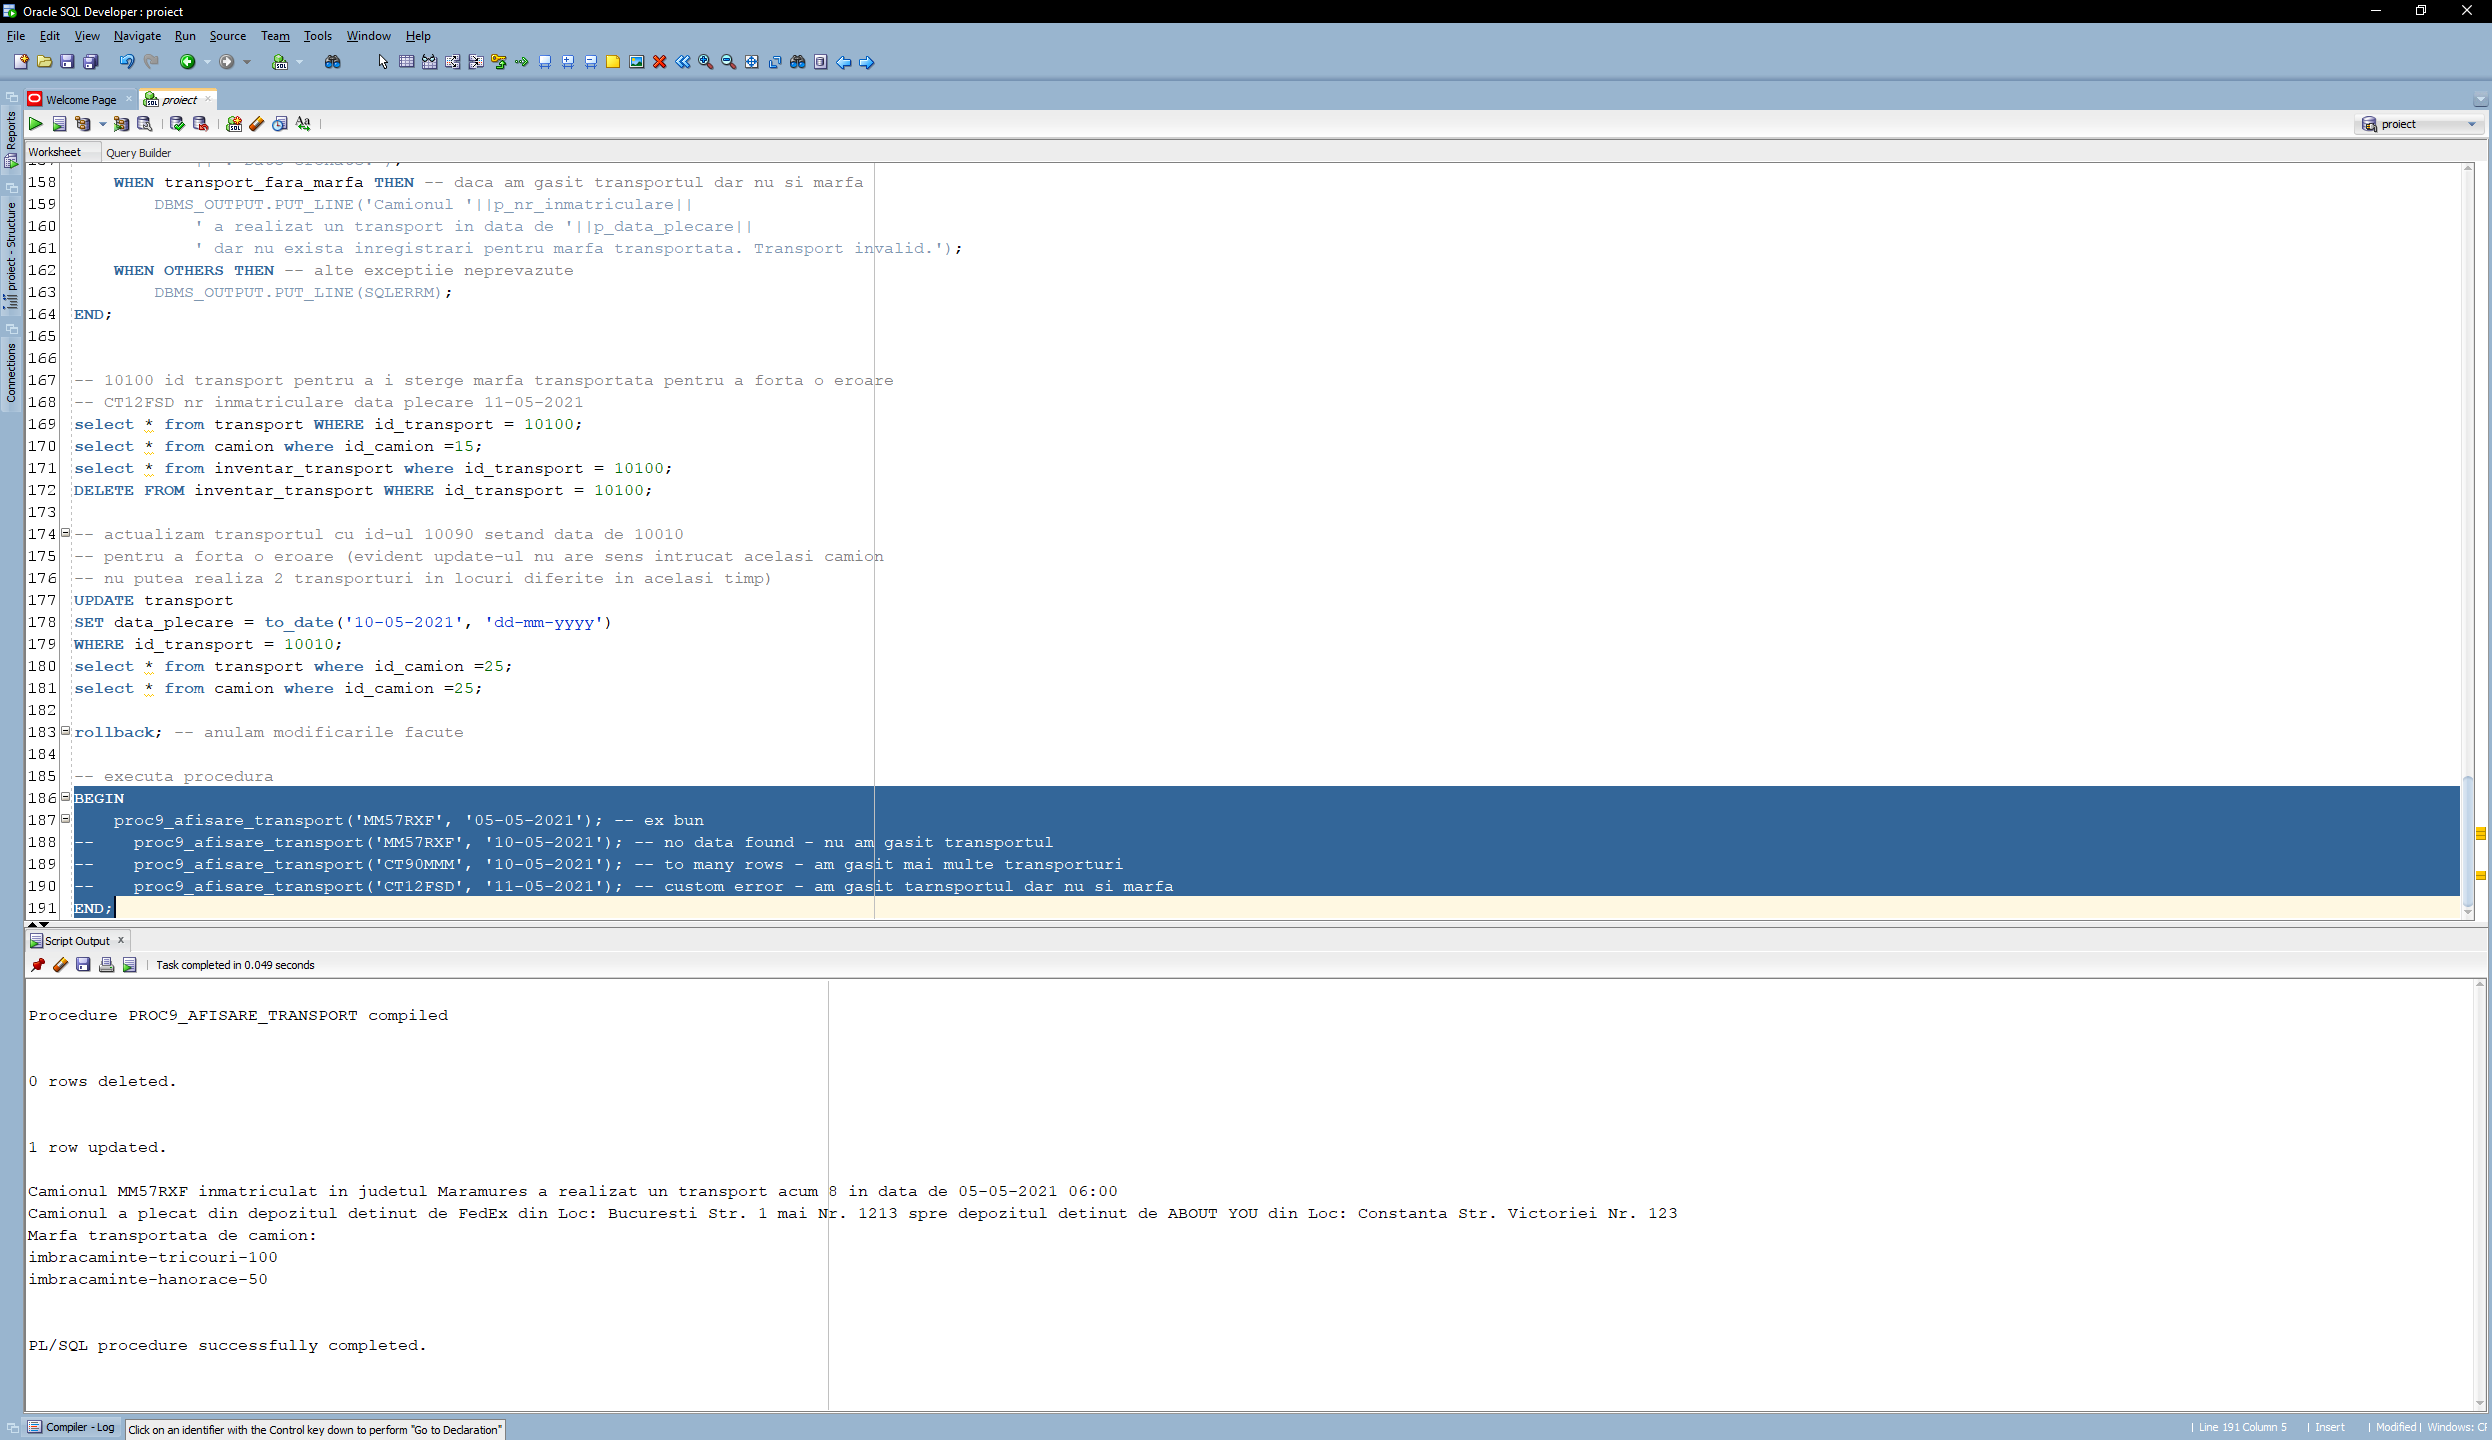
\includegraphics[width=\textwidth]{9_1.png}

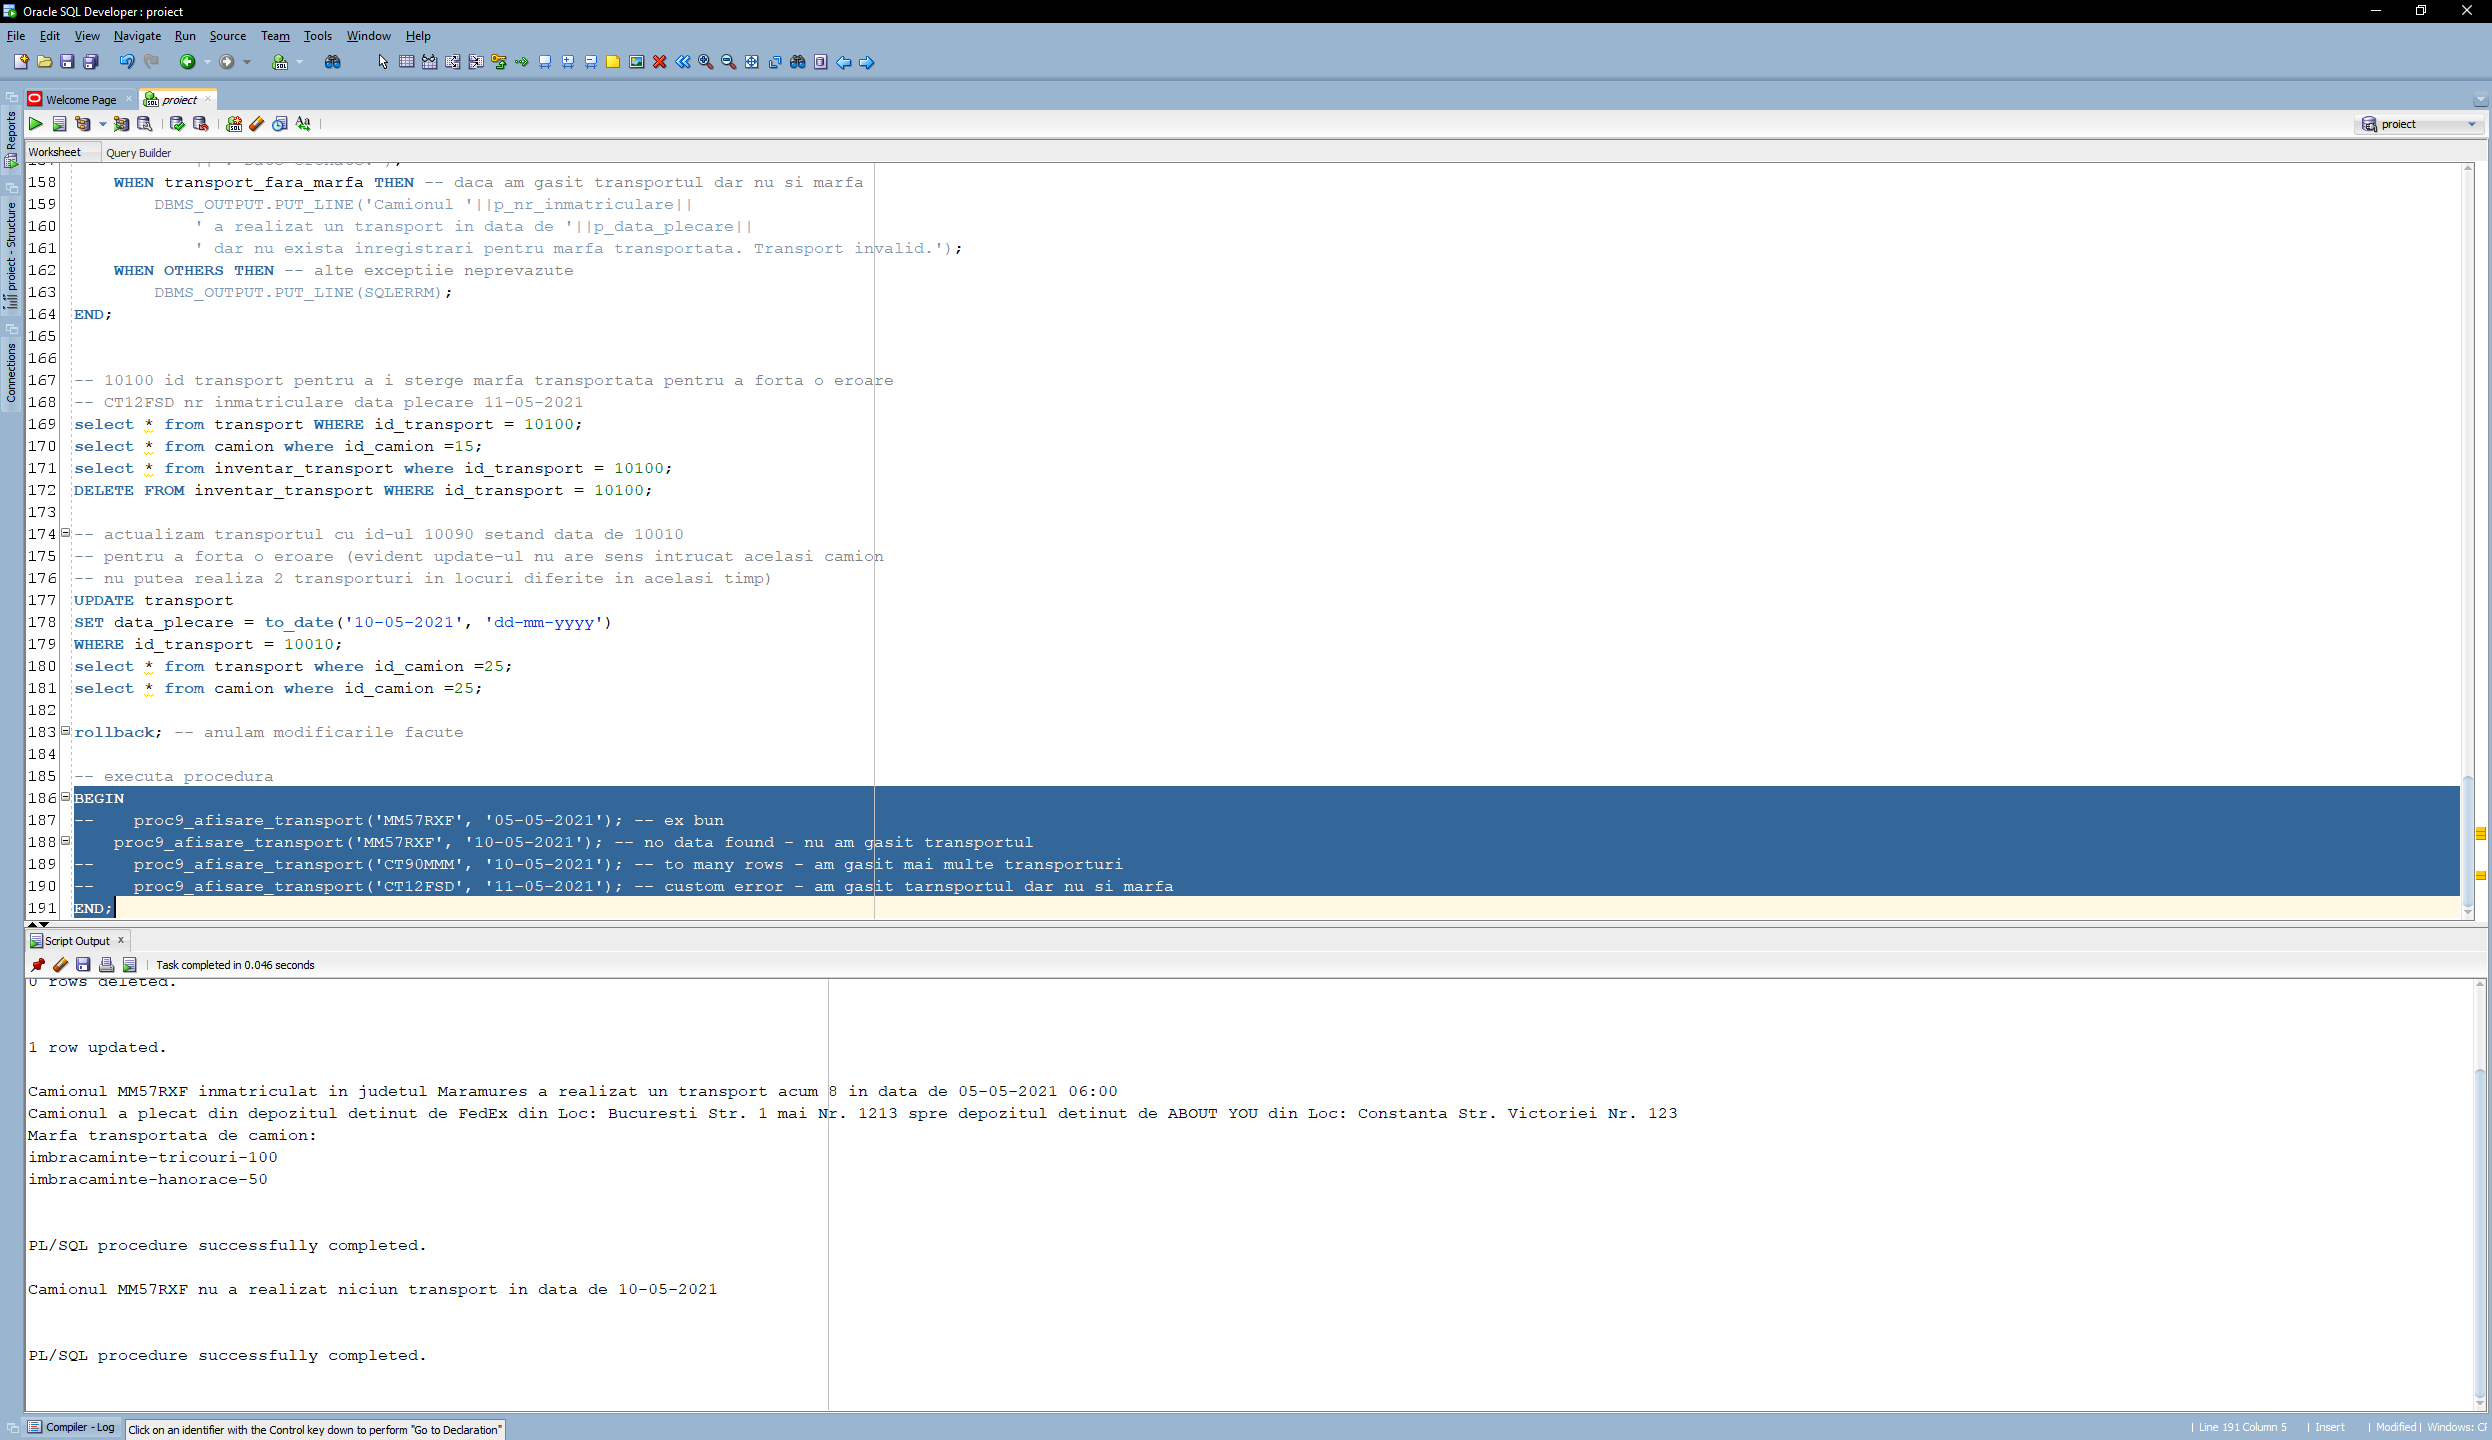
\includegraphics[width=\textwidth]{9_2.png}

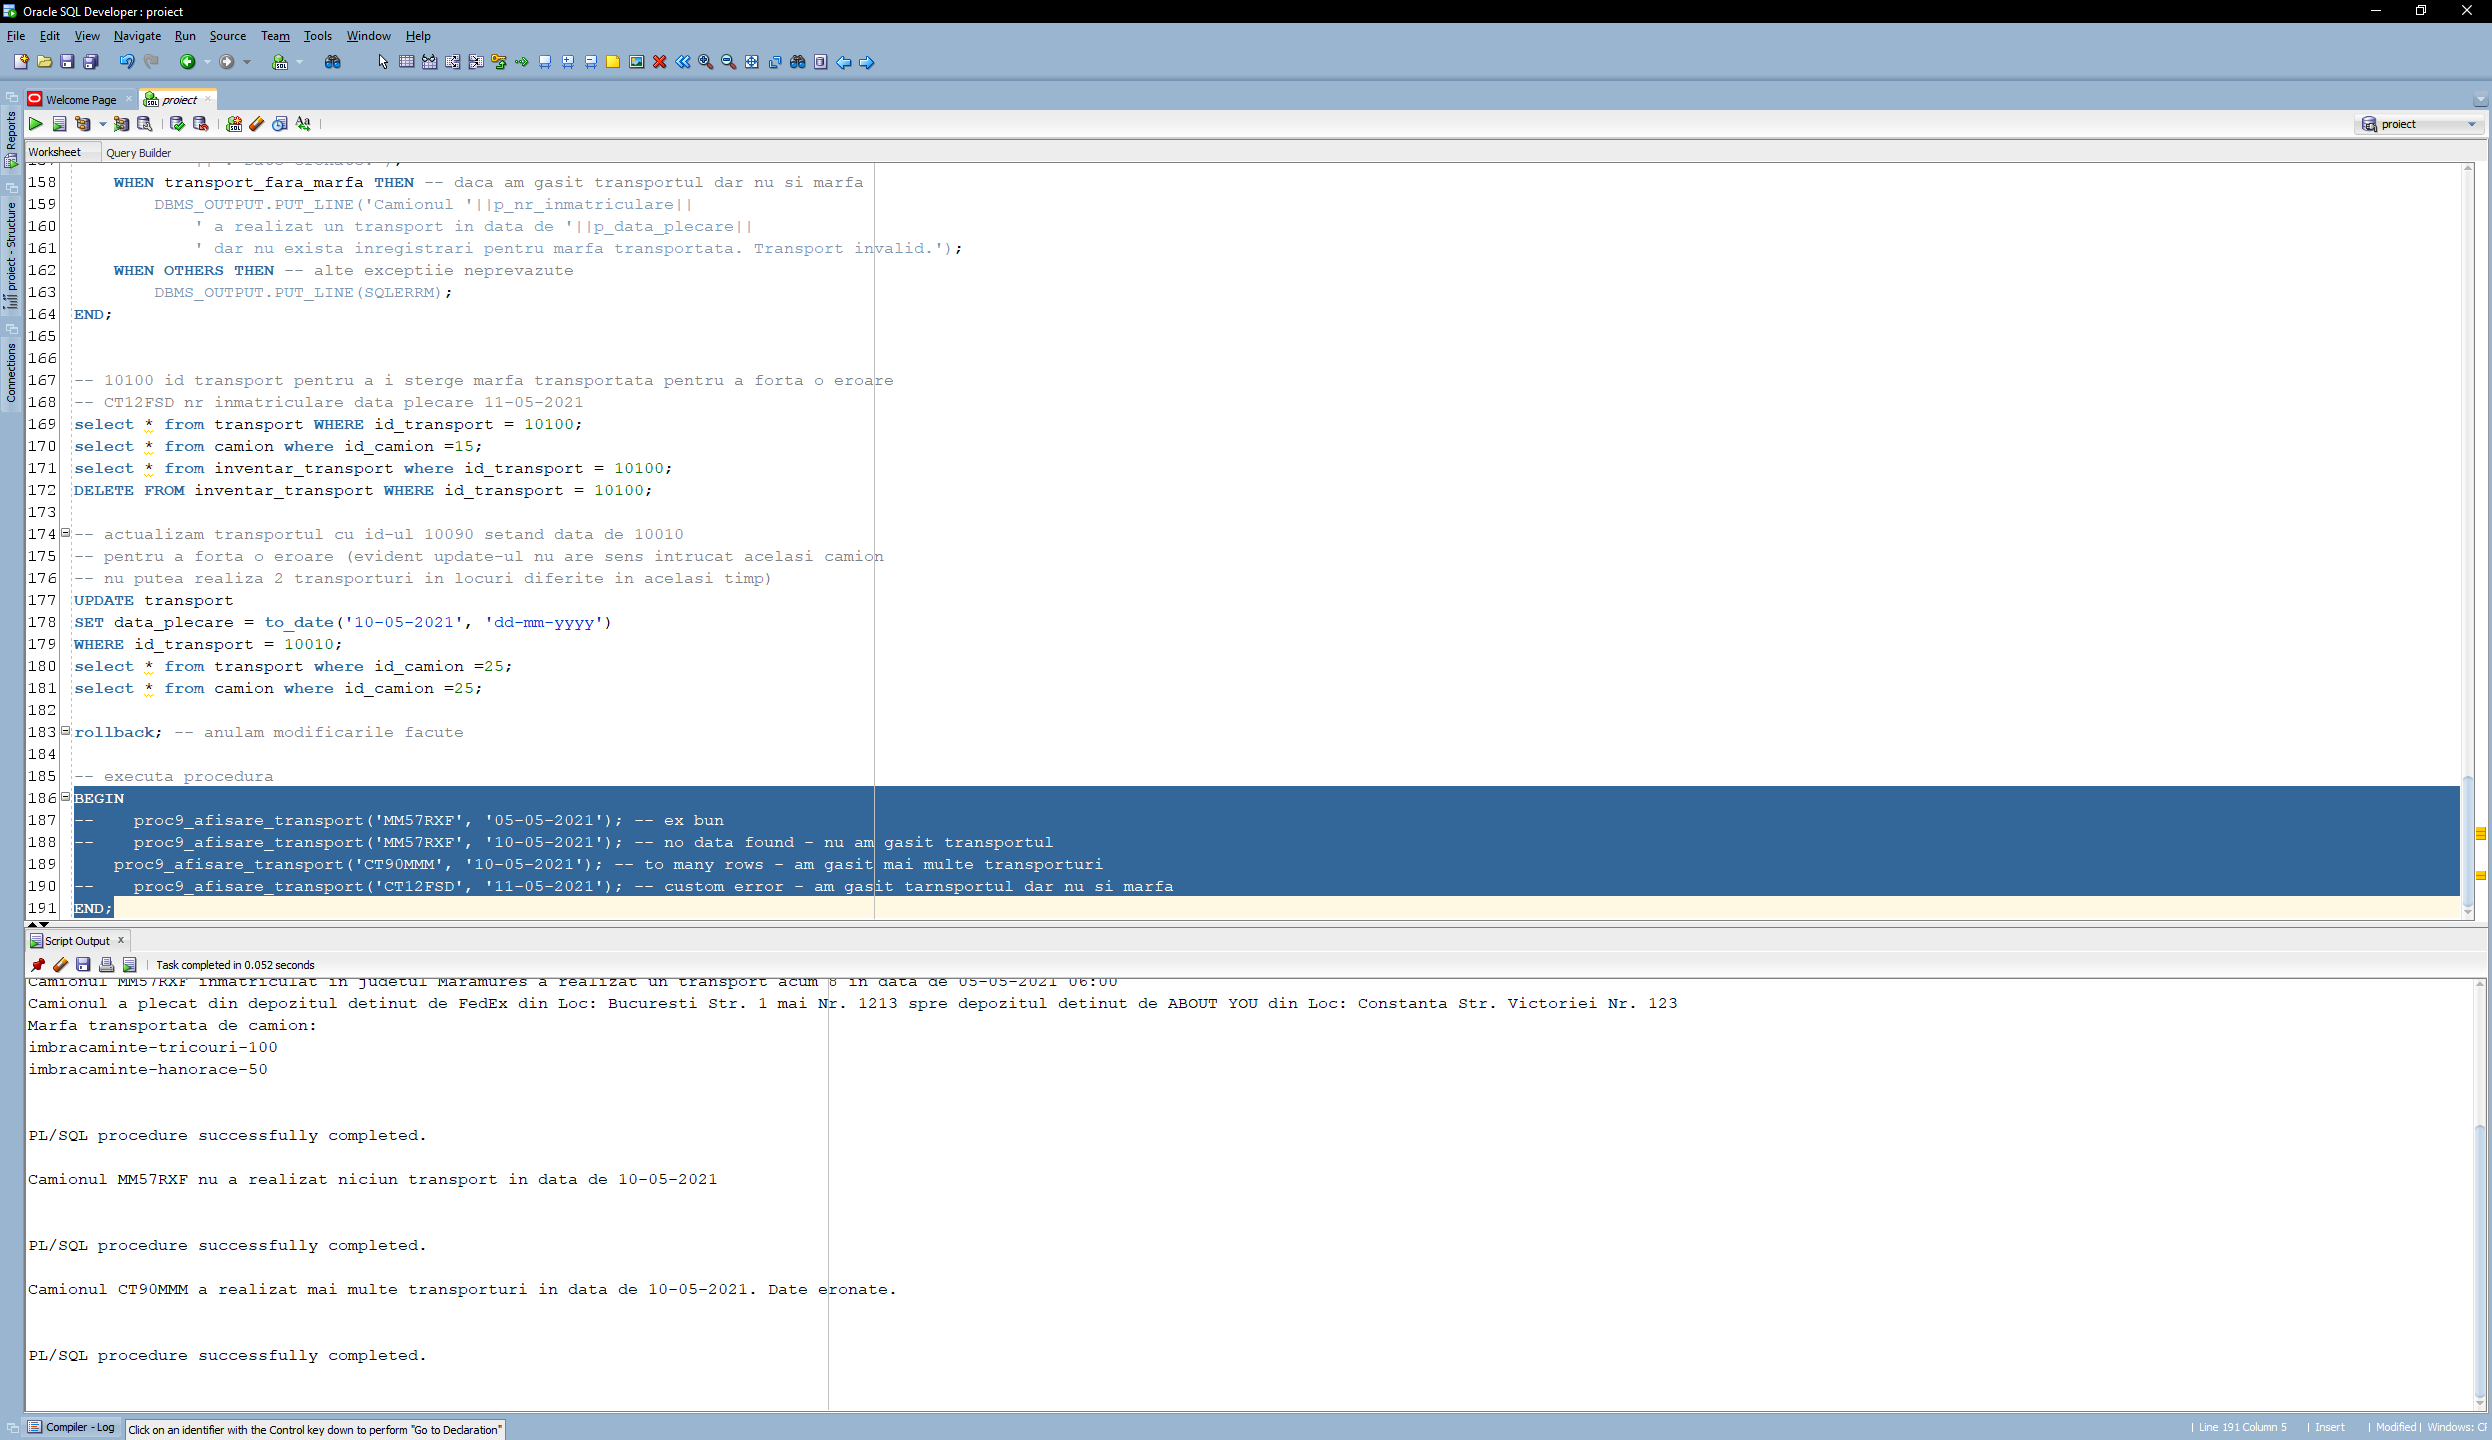
\includegraphics[width=\textwidth]{9_3.png}

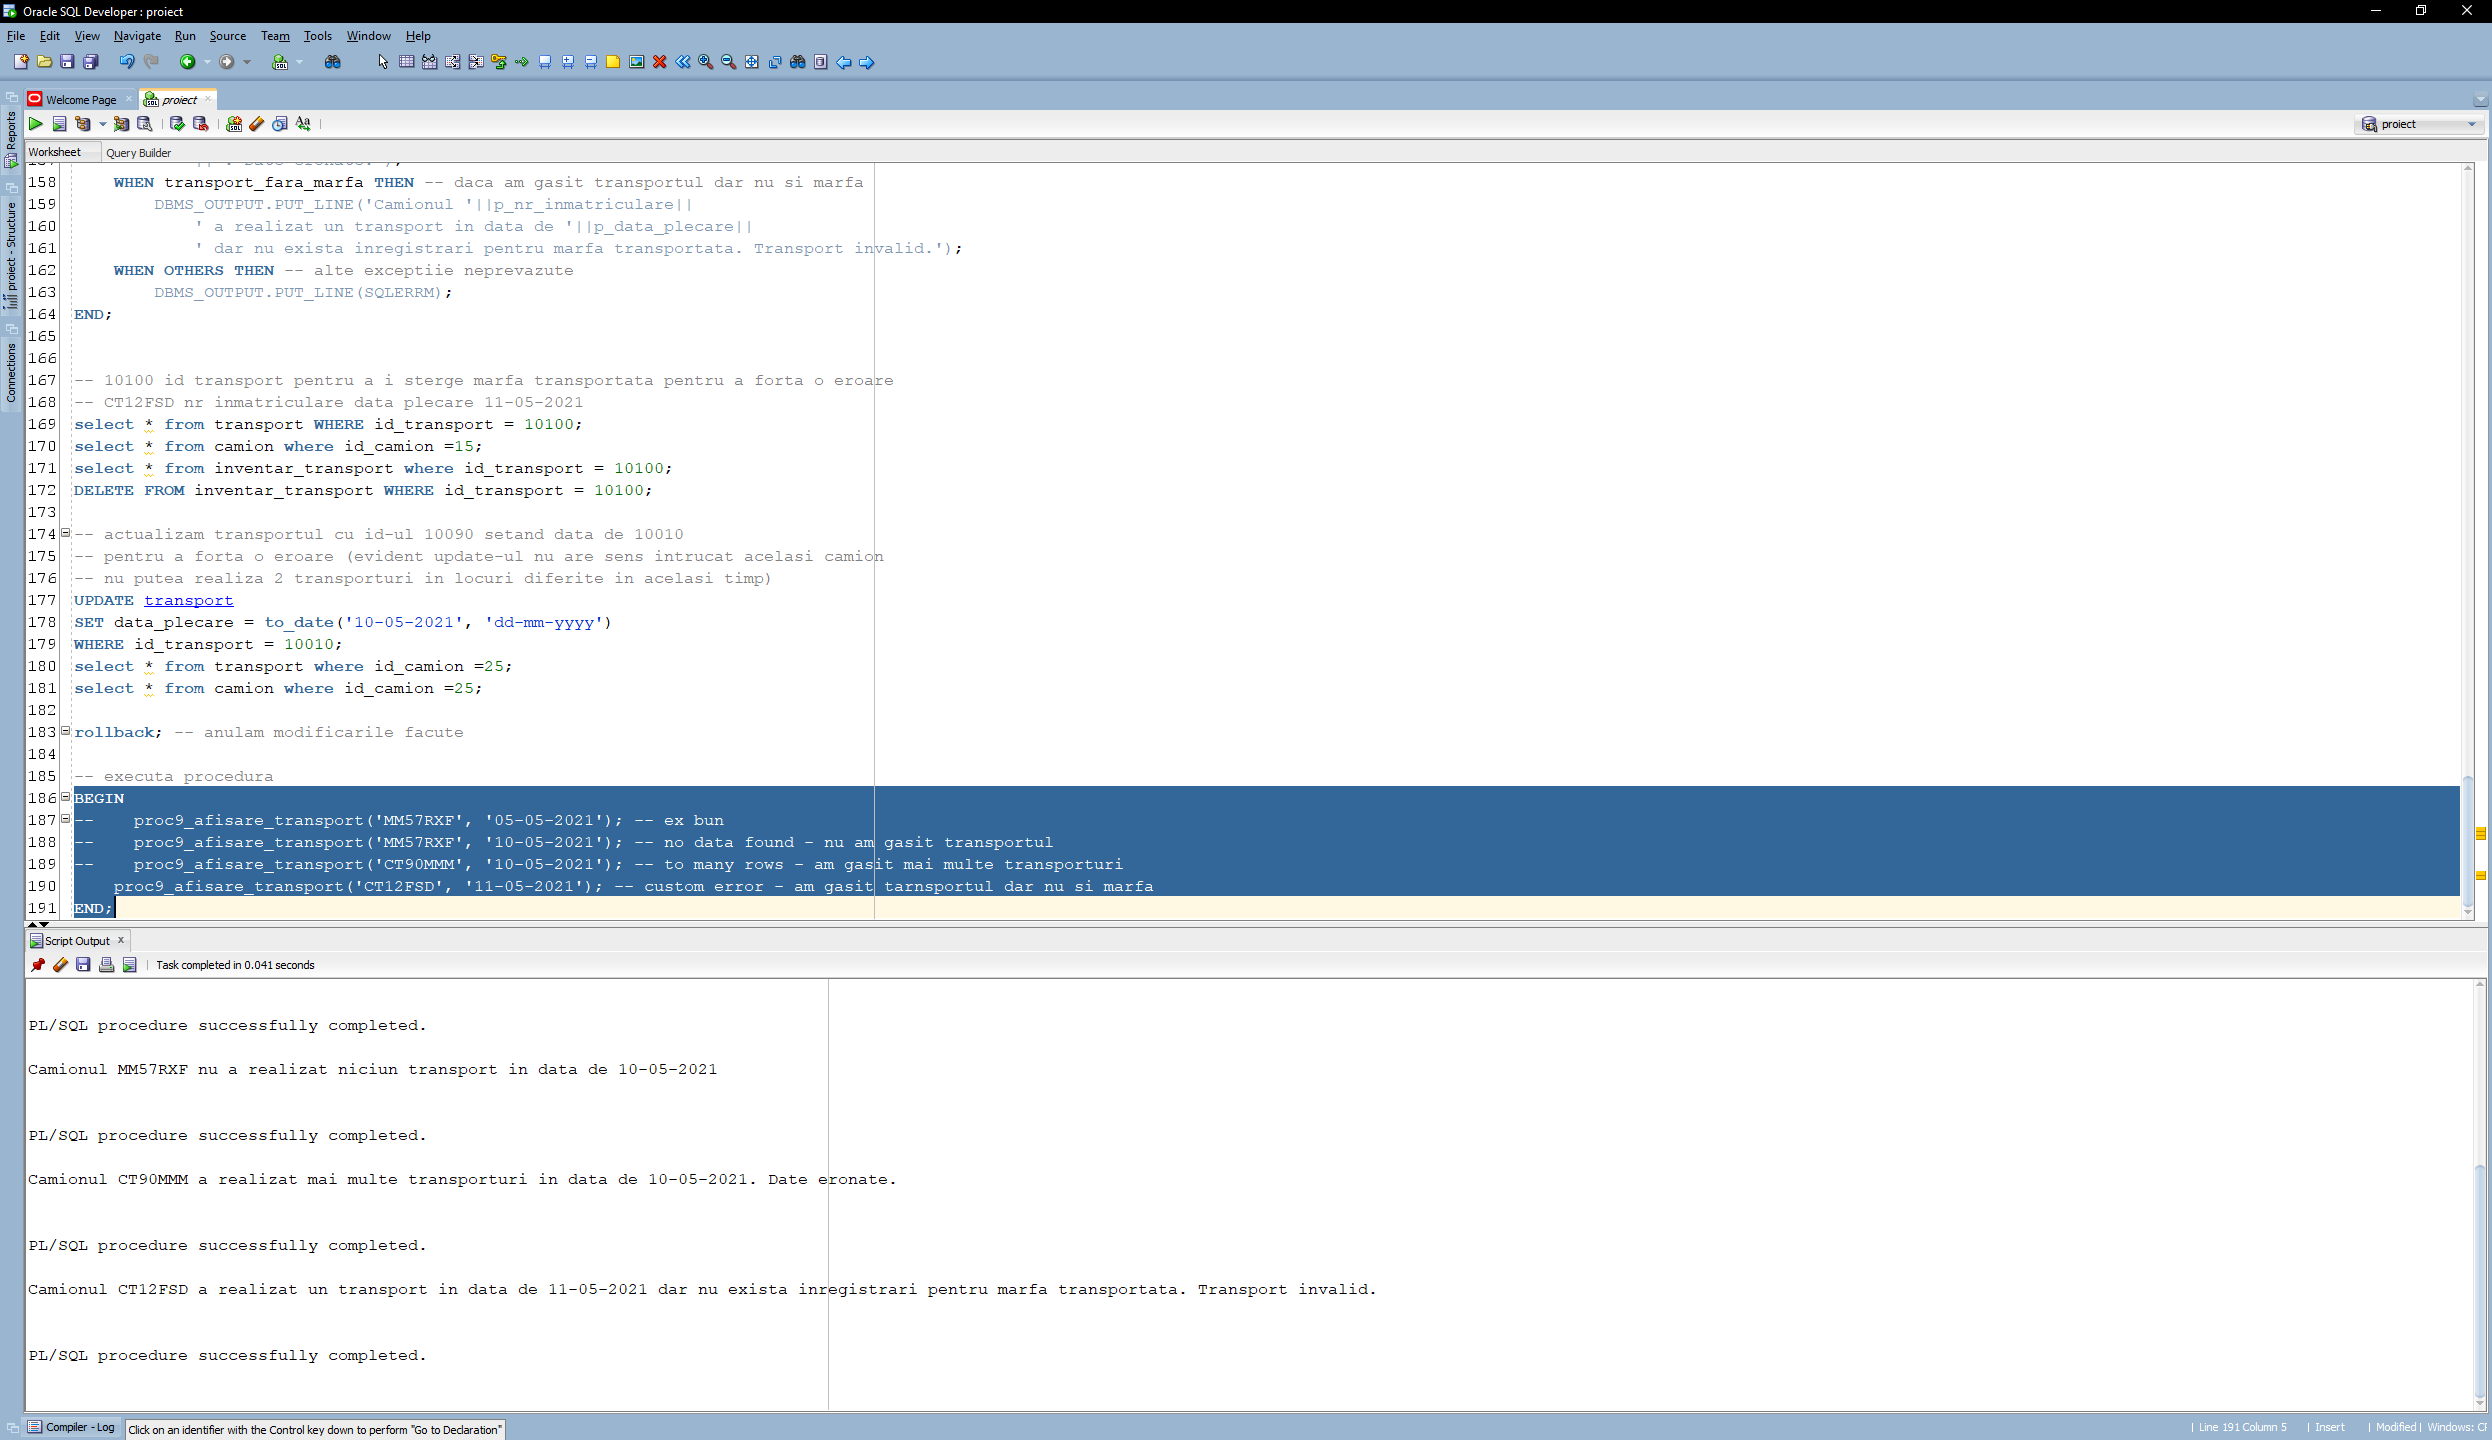
\includegraphics[width=\textwidth]{9_4.png}

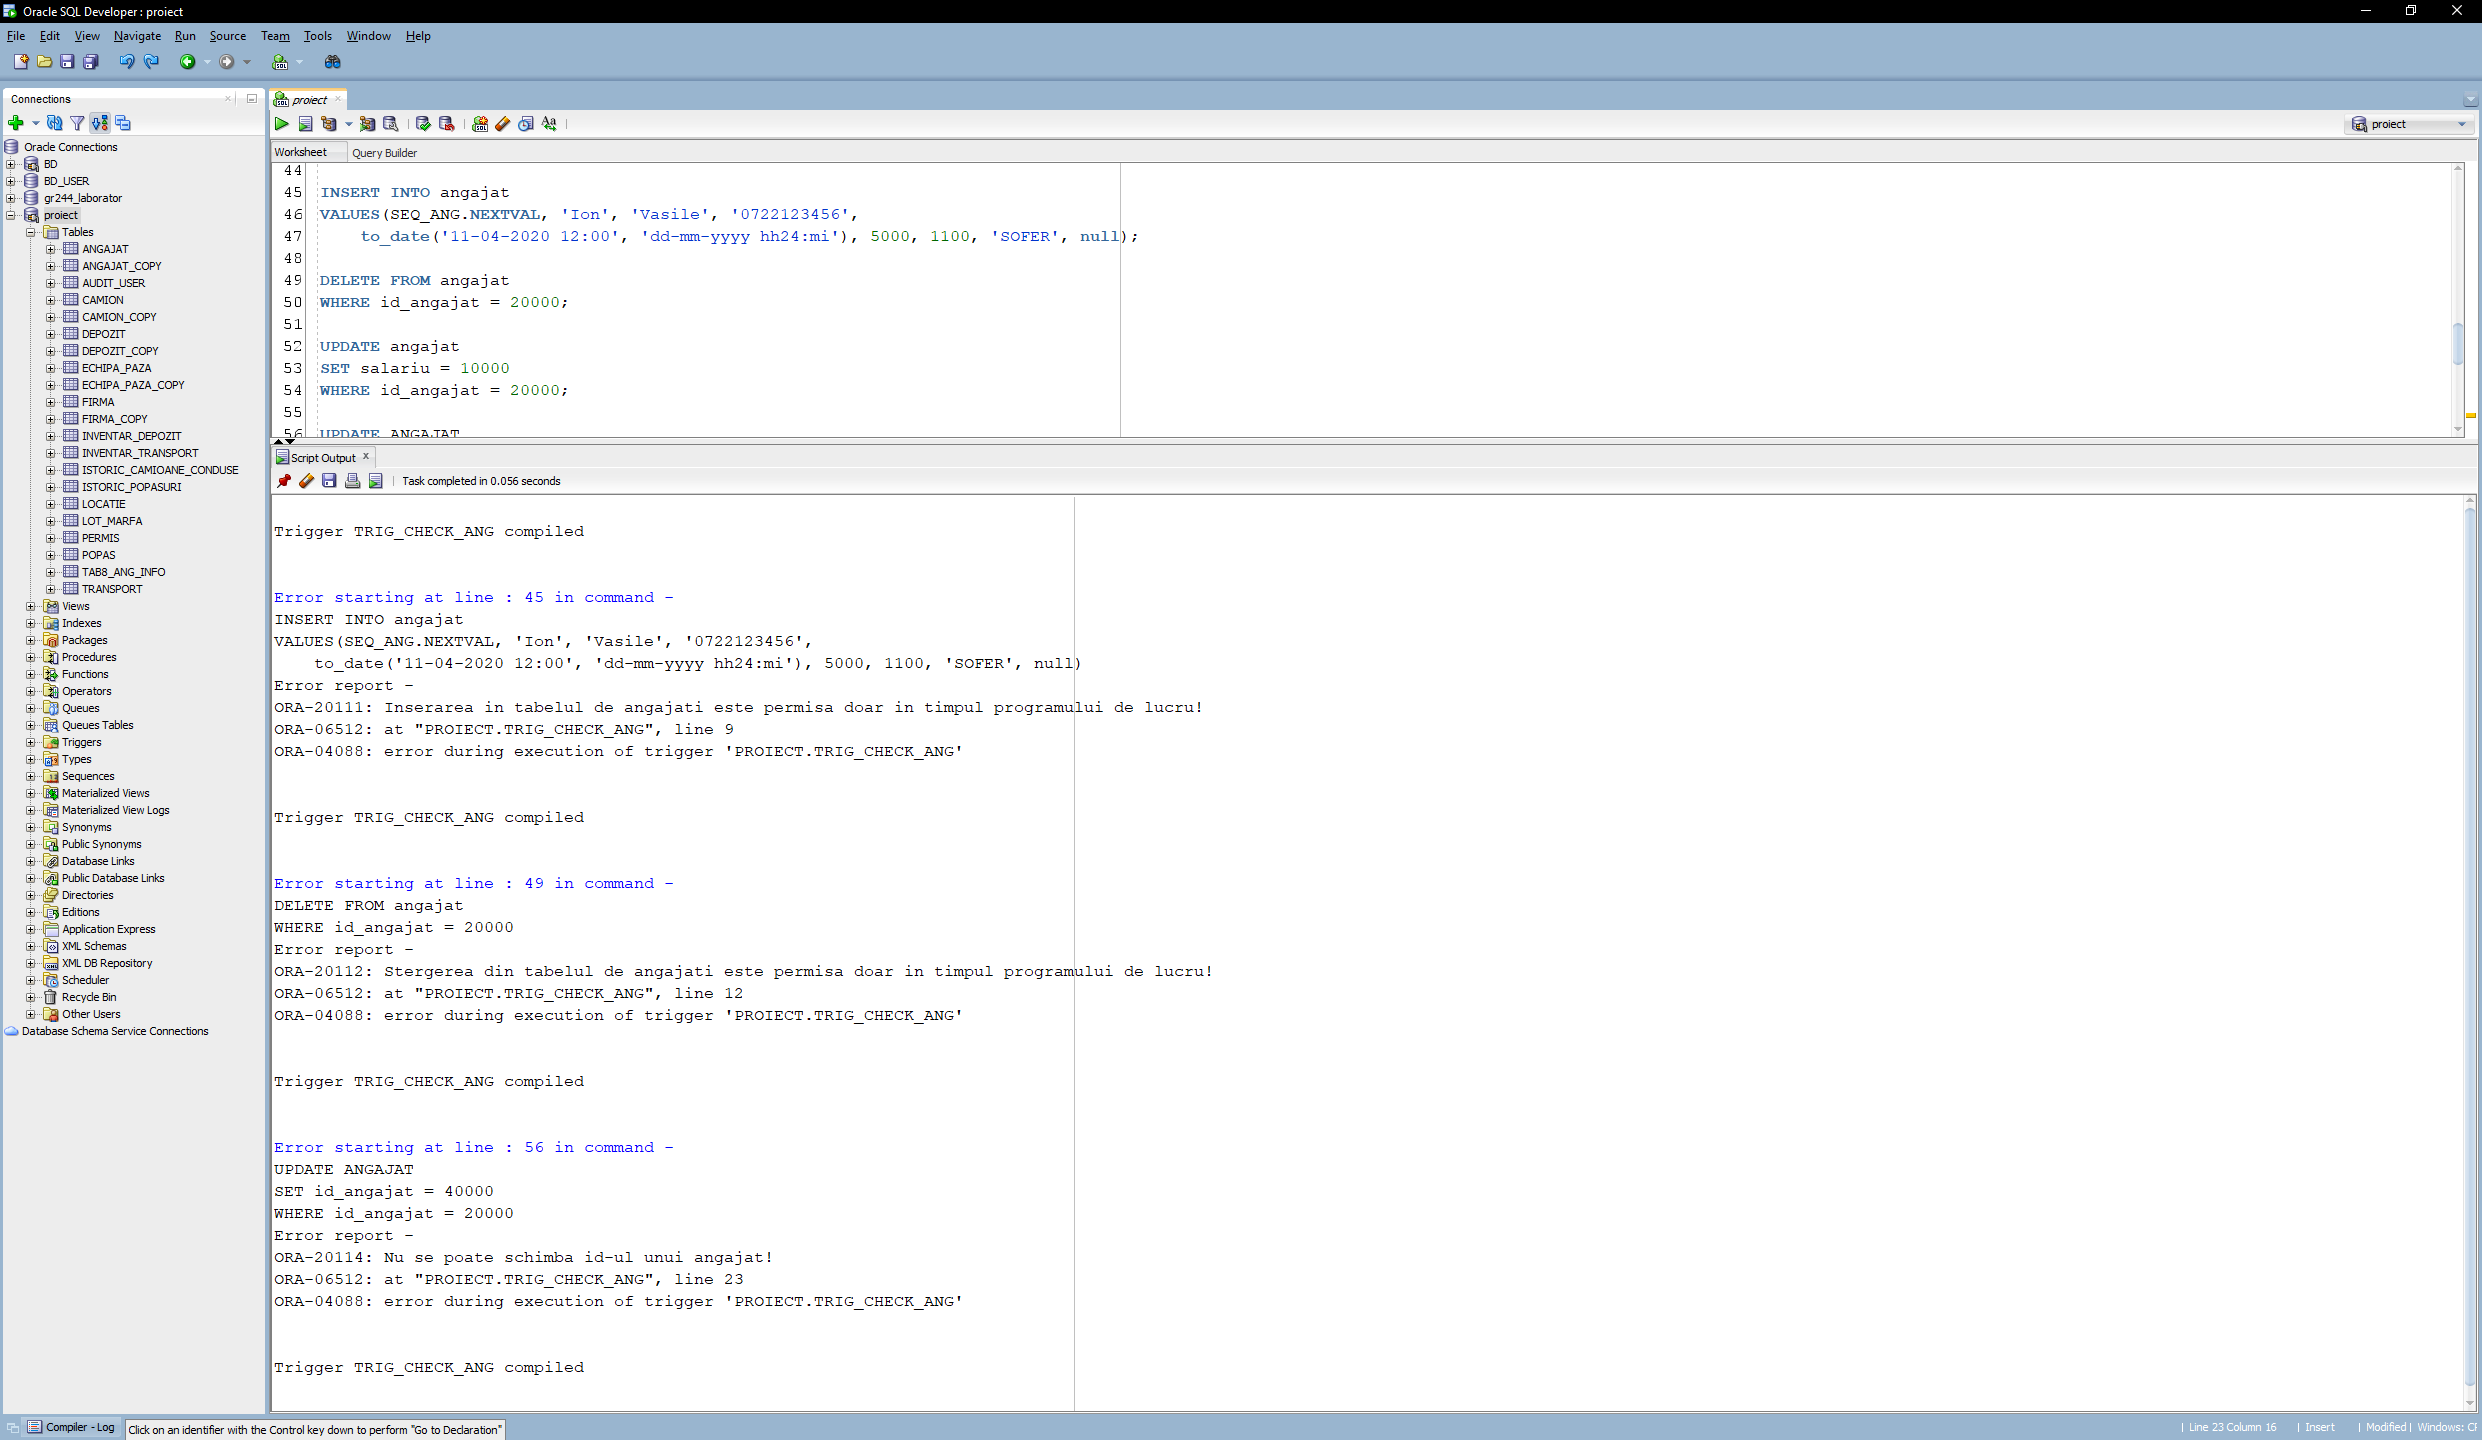
\includegraphics[width=\textwidth]{100_1.png}

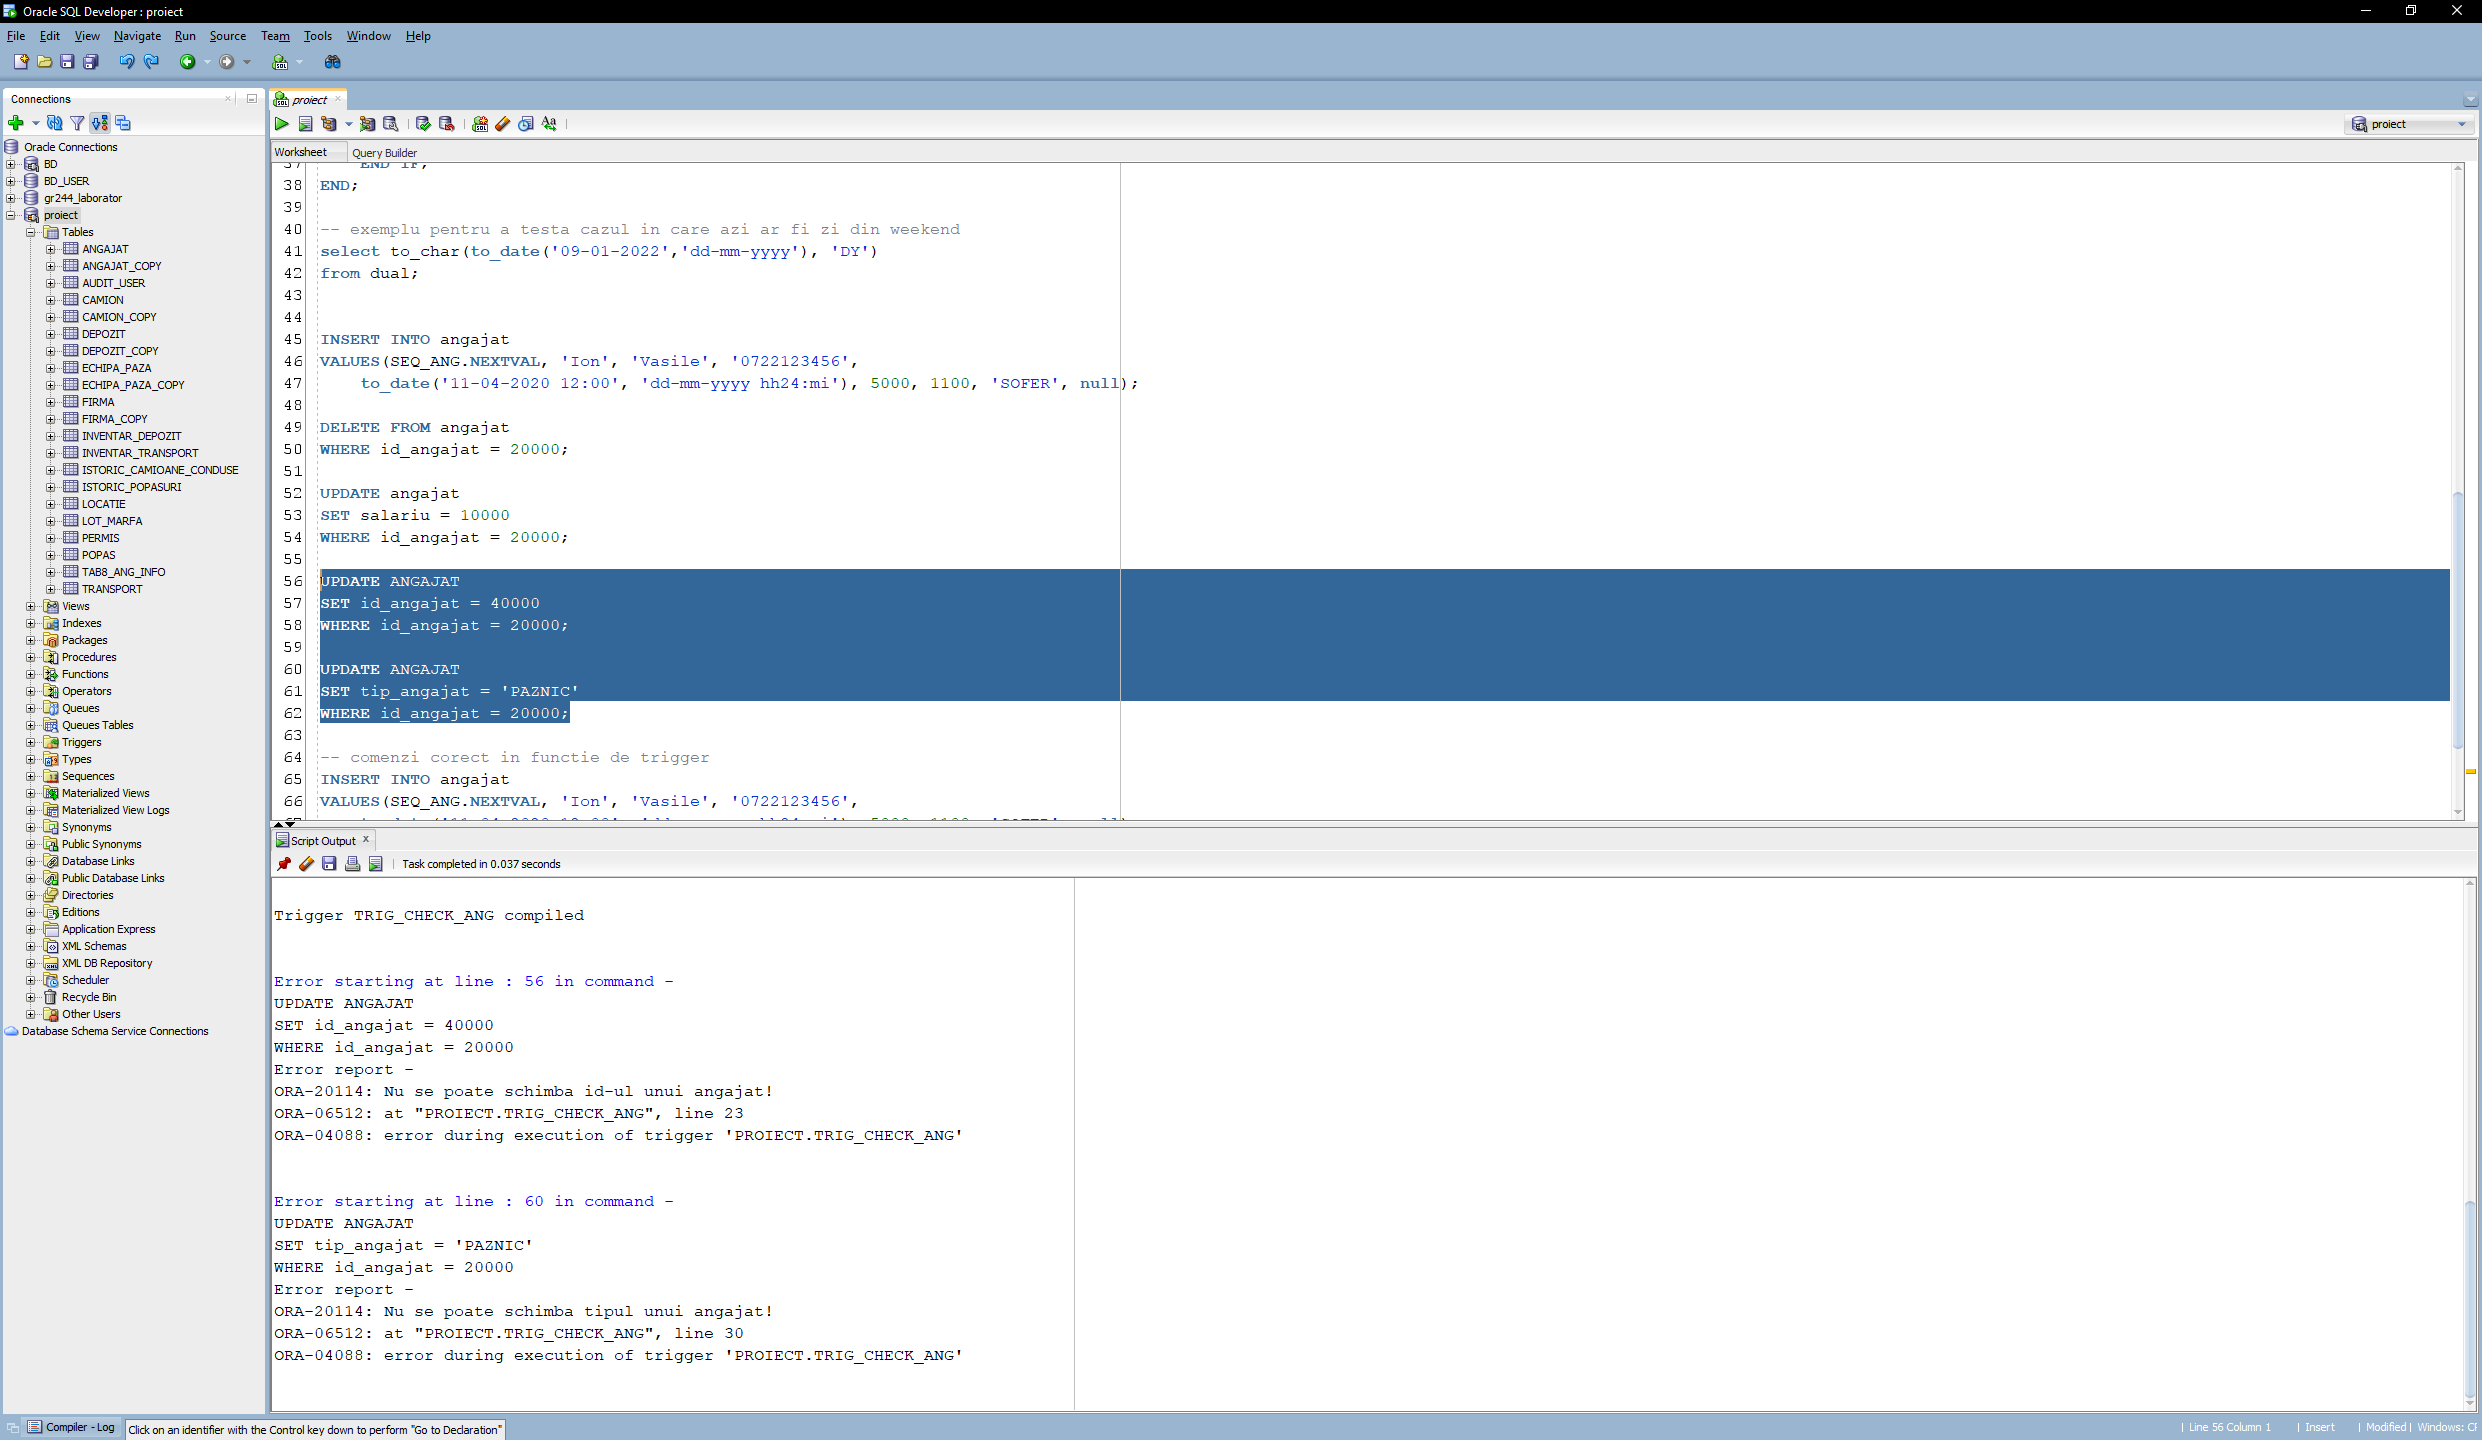
\includegraphics[width=\textwidth]{100_2.png}

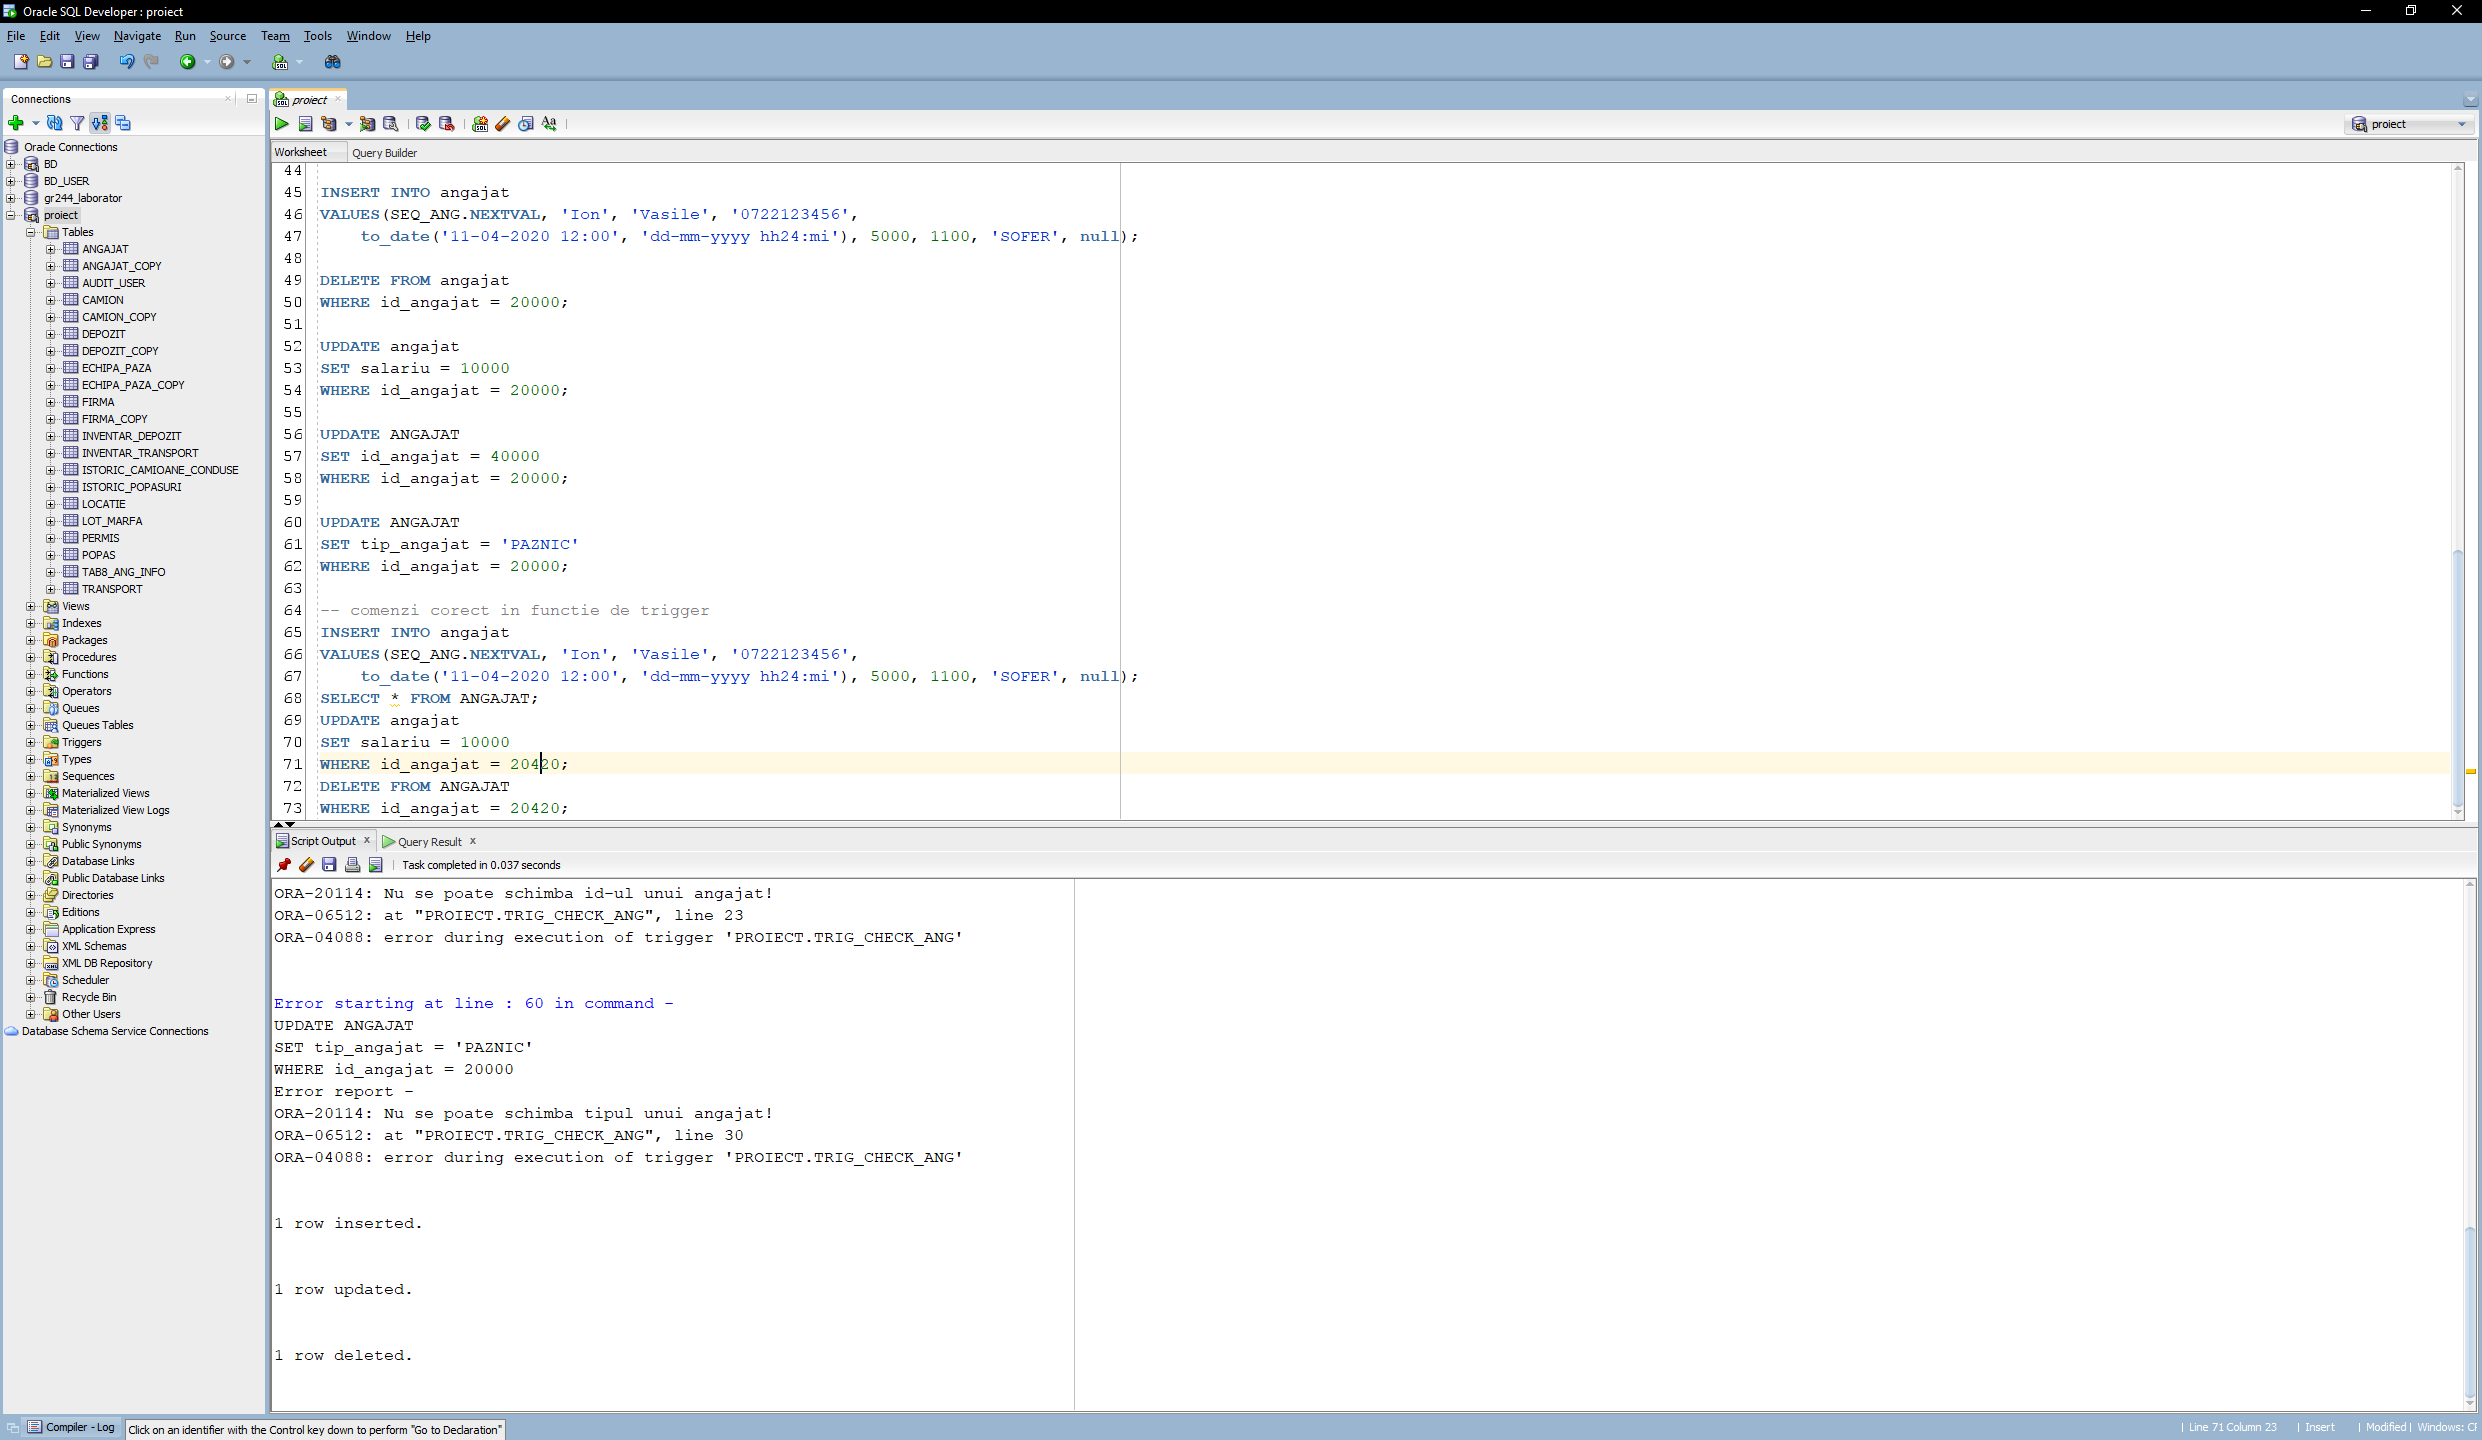
\includegraphics[width=\textwidth]{100_3.png}

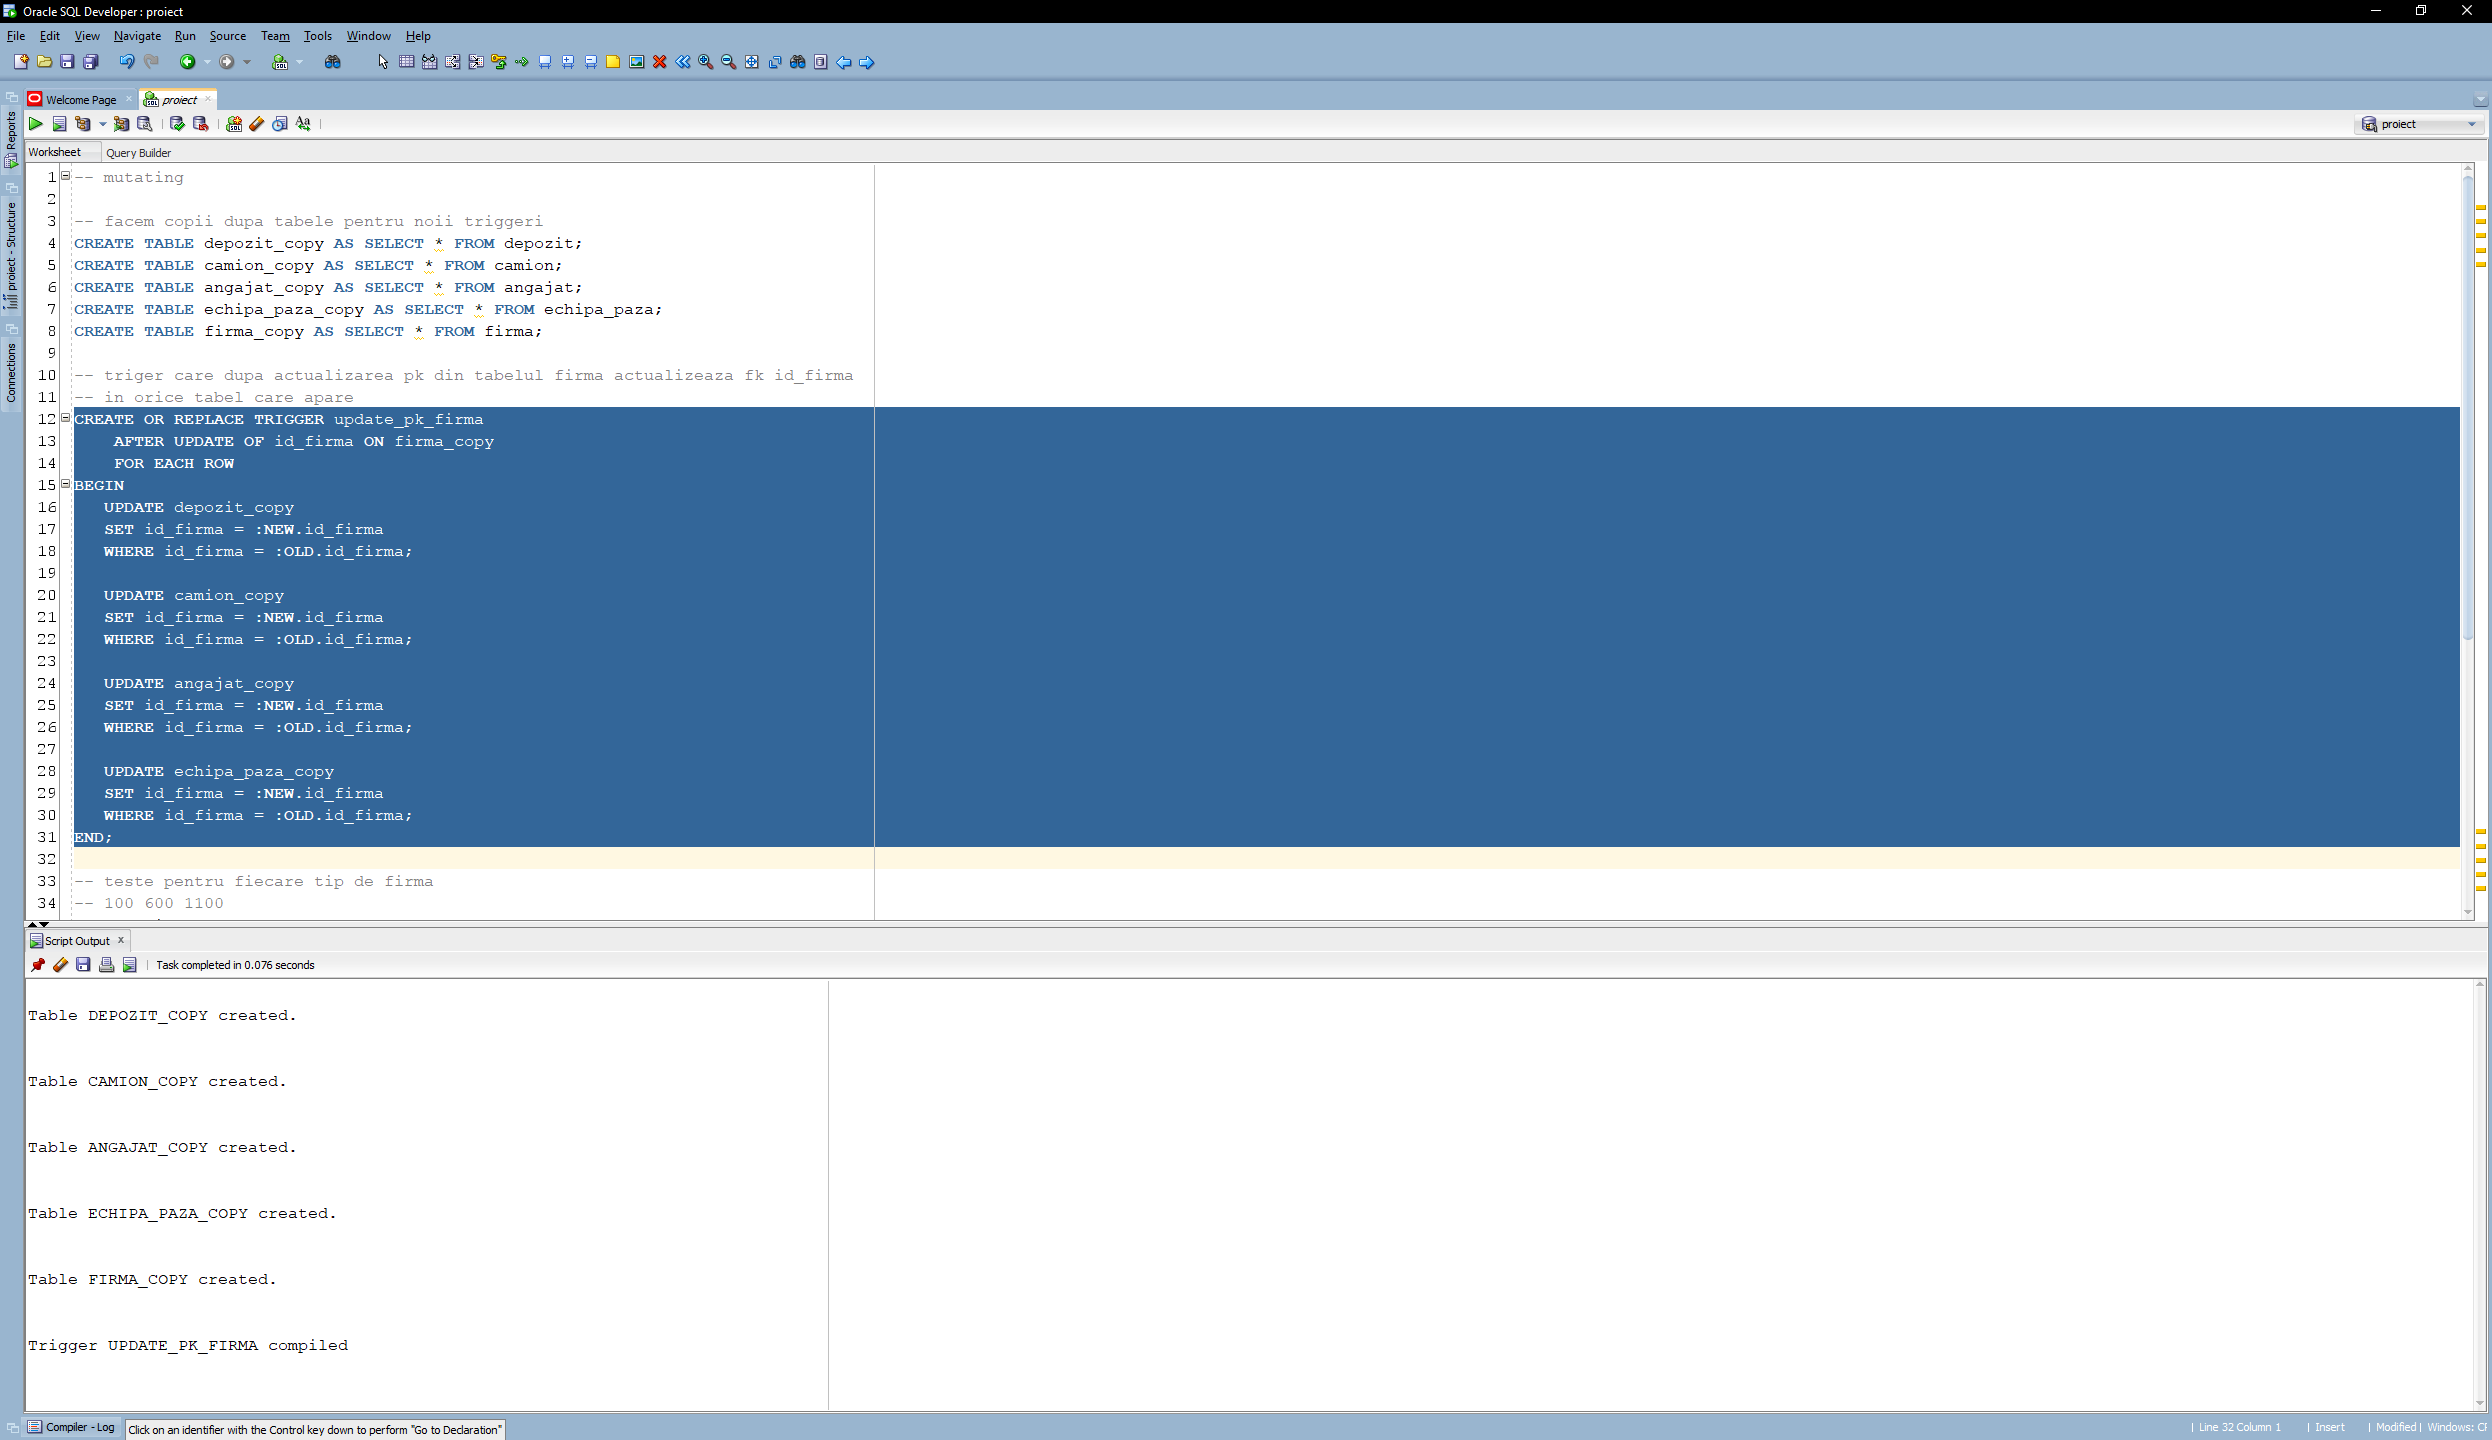
\includegraphics[width=\textwidth]{10_1.png}

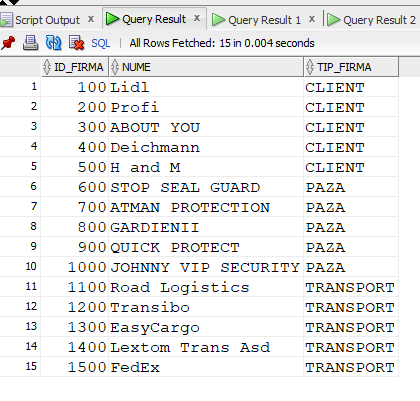
\includegraphics[width=\textwidth]{10_2.png}

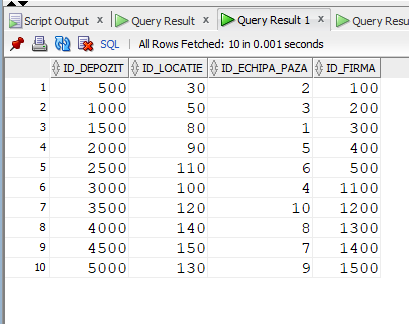
\includegraphics[width=\textwidth]{10_3.png}

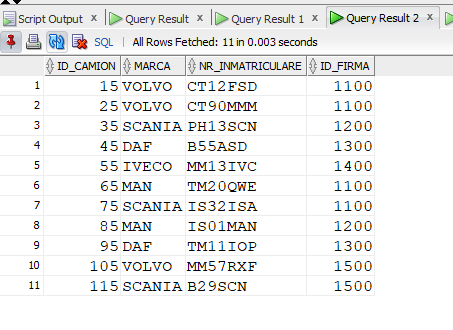
\includegraphics[width=\textwidth]{10_4.png}

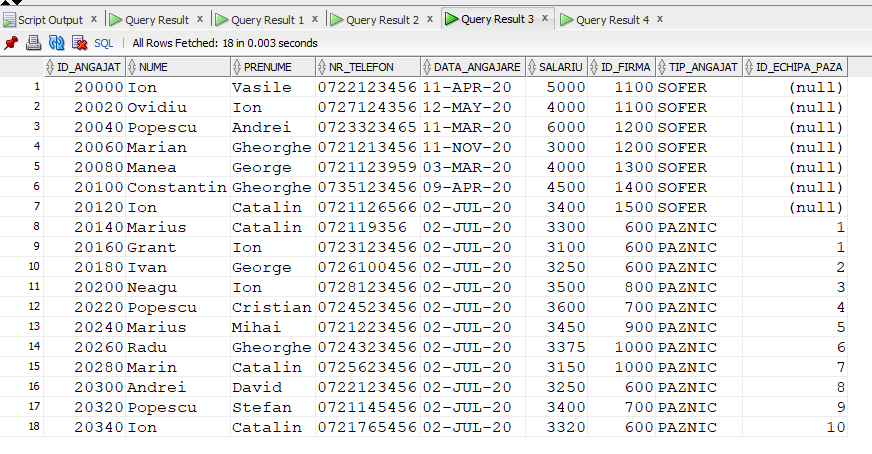
\includegraphics[width=\textwidth]{10_5.png}

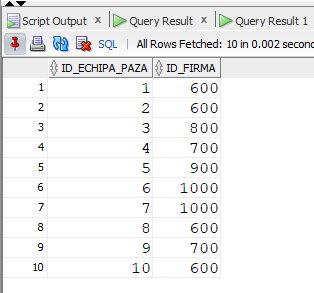
\includegraphics[width=\textwidth]{10_6.png}

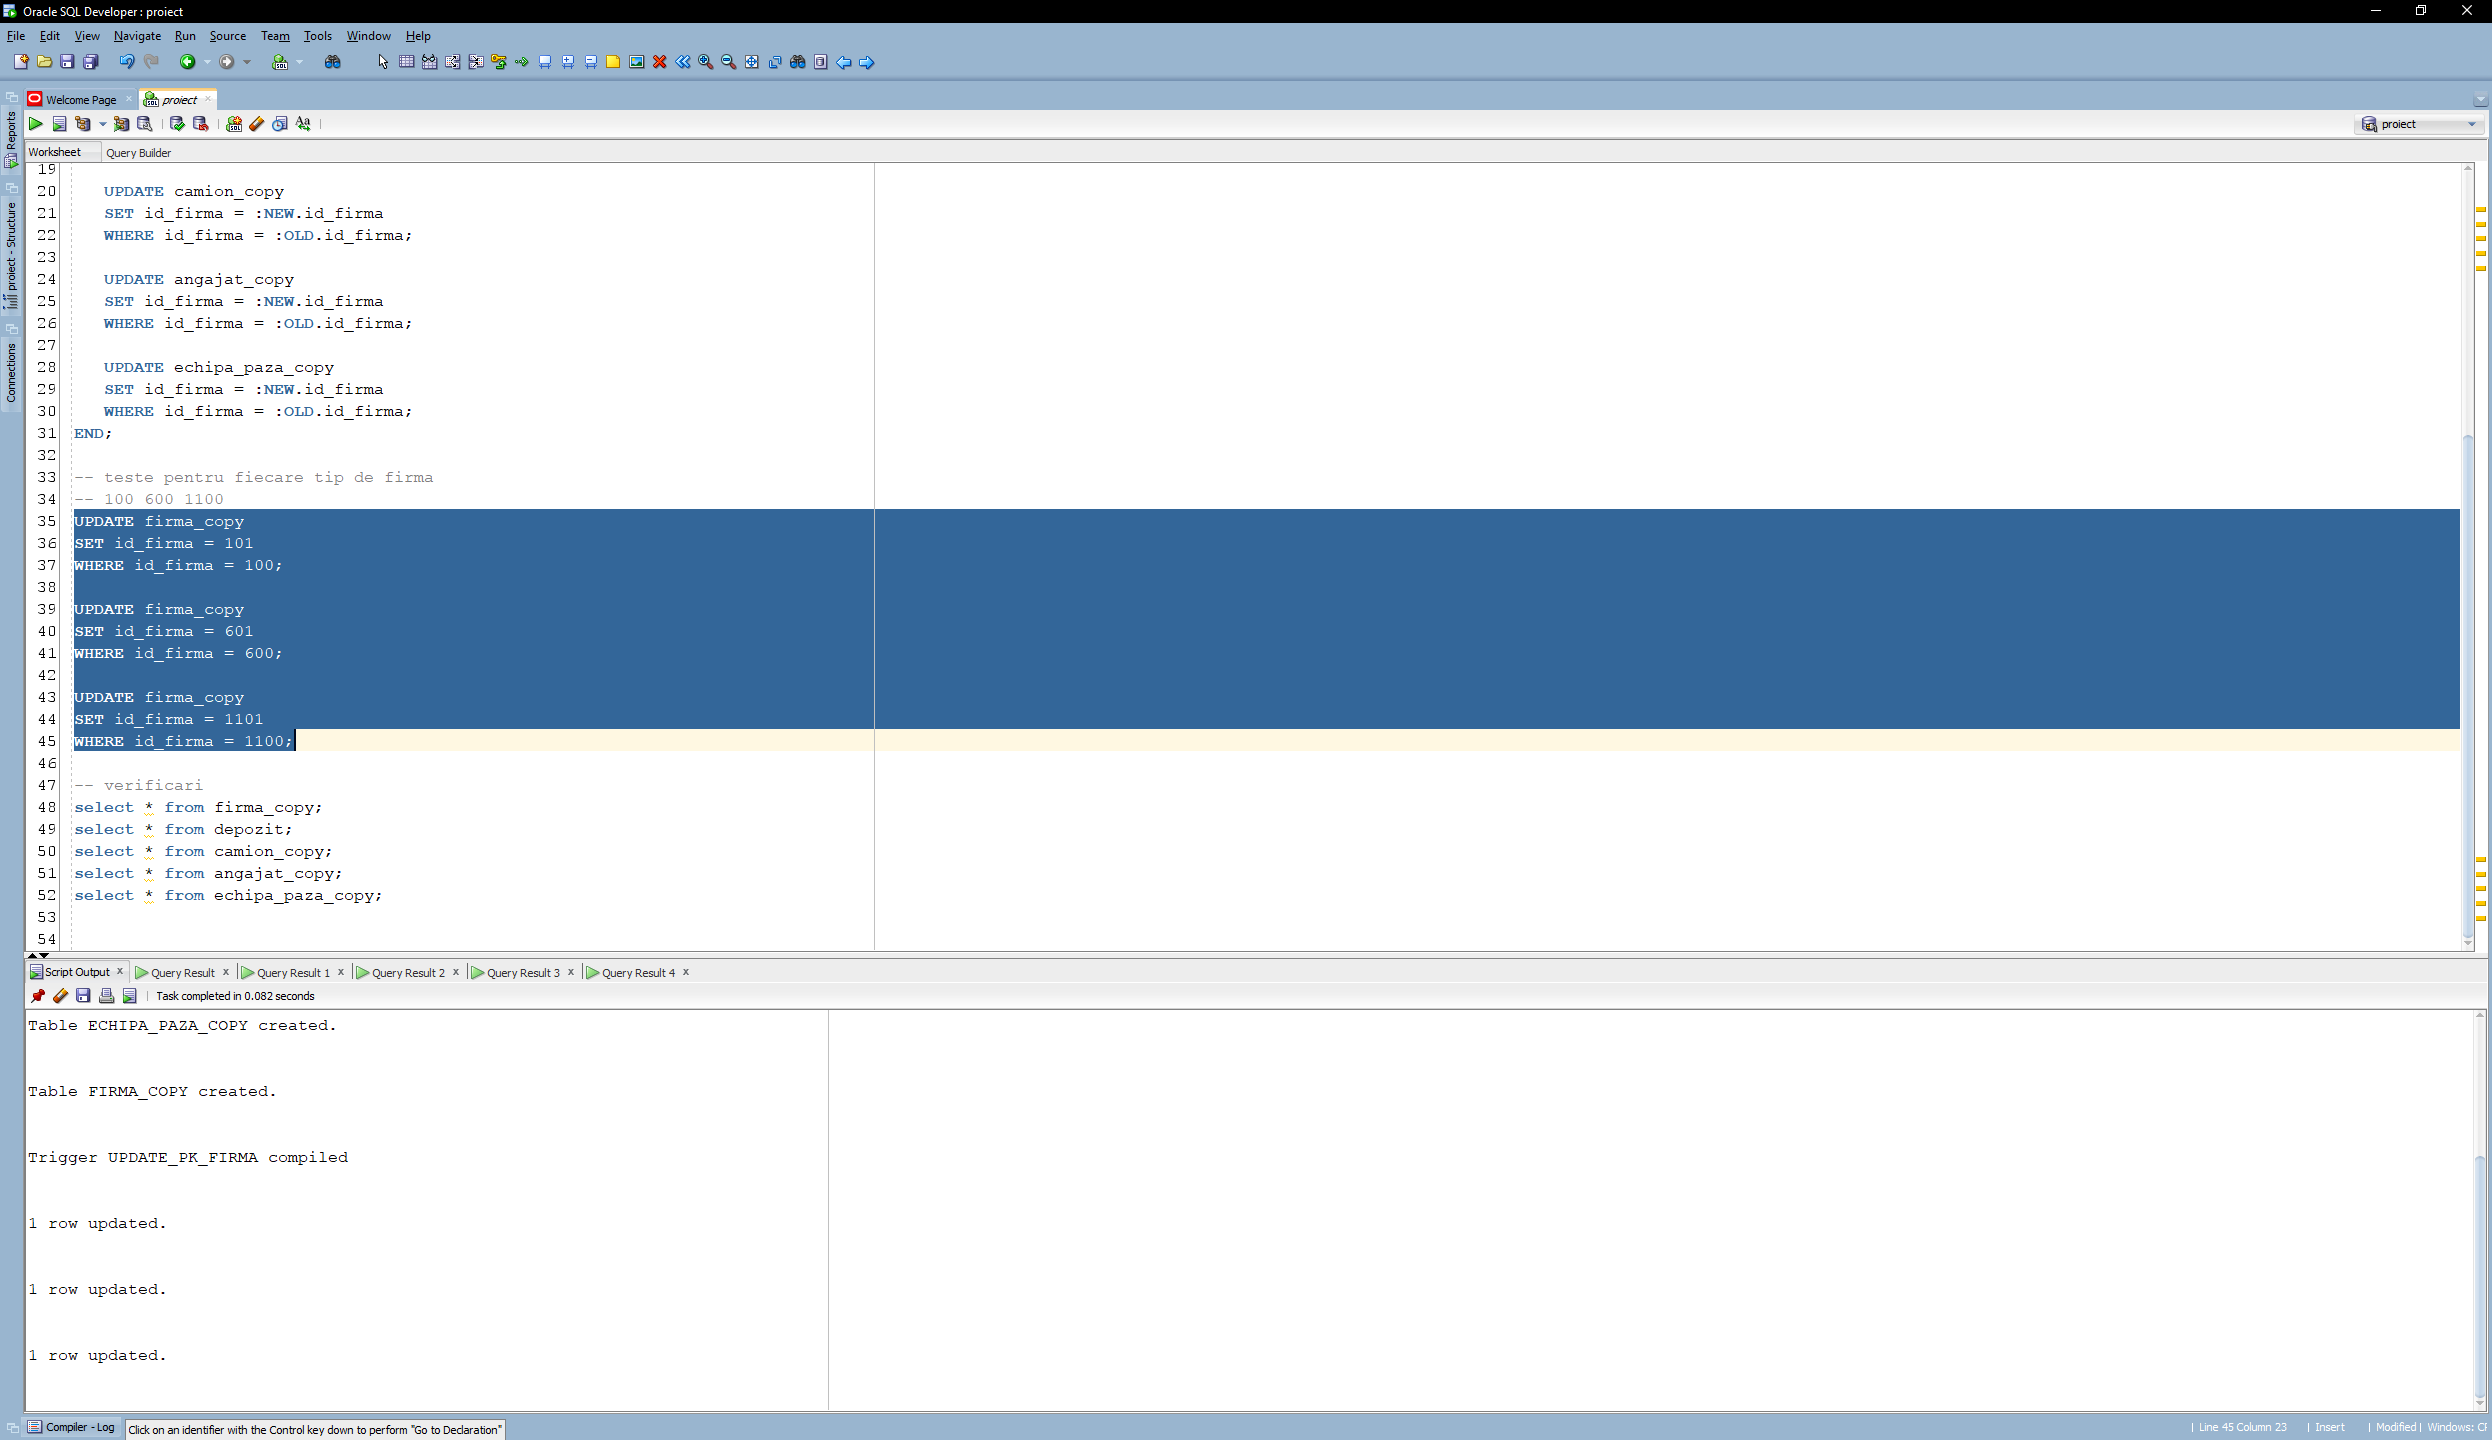
\includegraphics[width=\textwidth]{10_7.png}

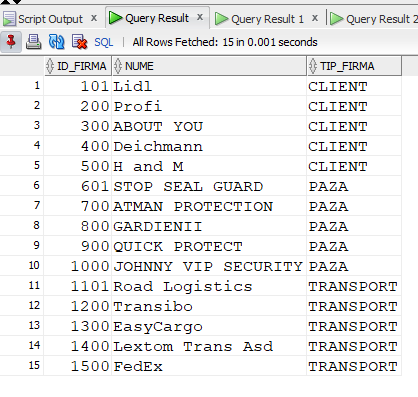
\includegraphics[width=\textwidth]{10_8.png}

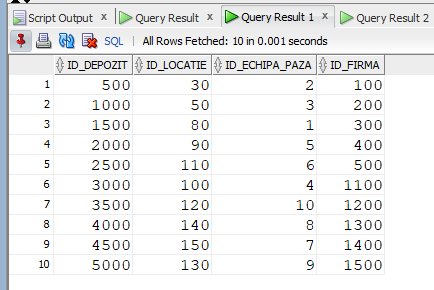
\includegraphics[width=\textwidth]{10_9.png}

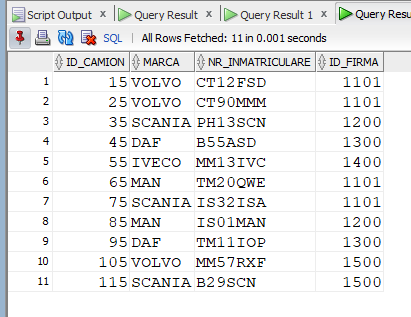
\includegraphics[width=\textwidth]{10_10.png}

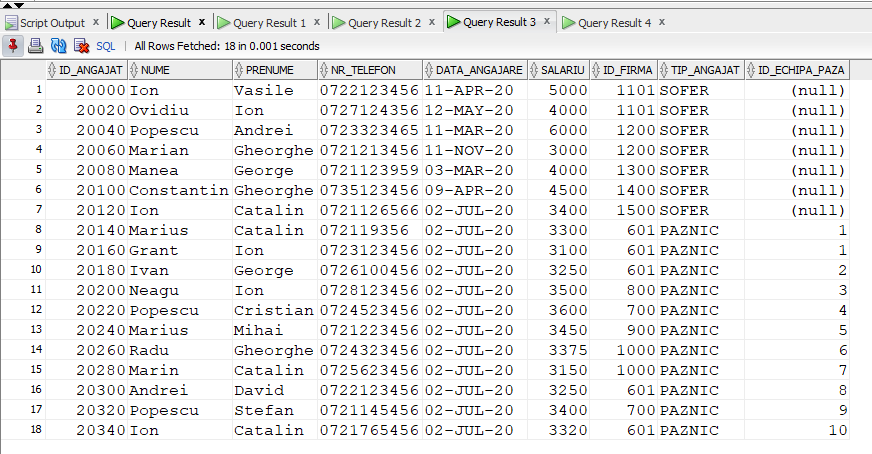
\includegraphics[width=\textwidth]{10_11.png}

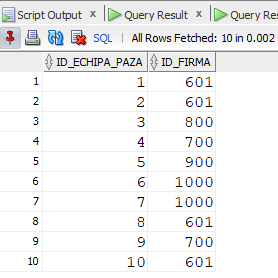
\includegraphics[width=\textwidth]{10_12.png}

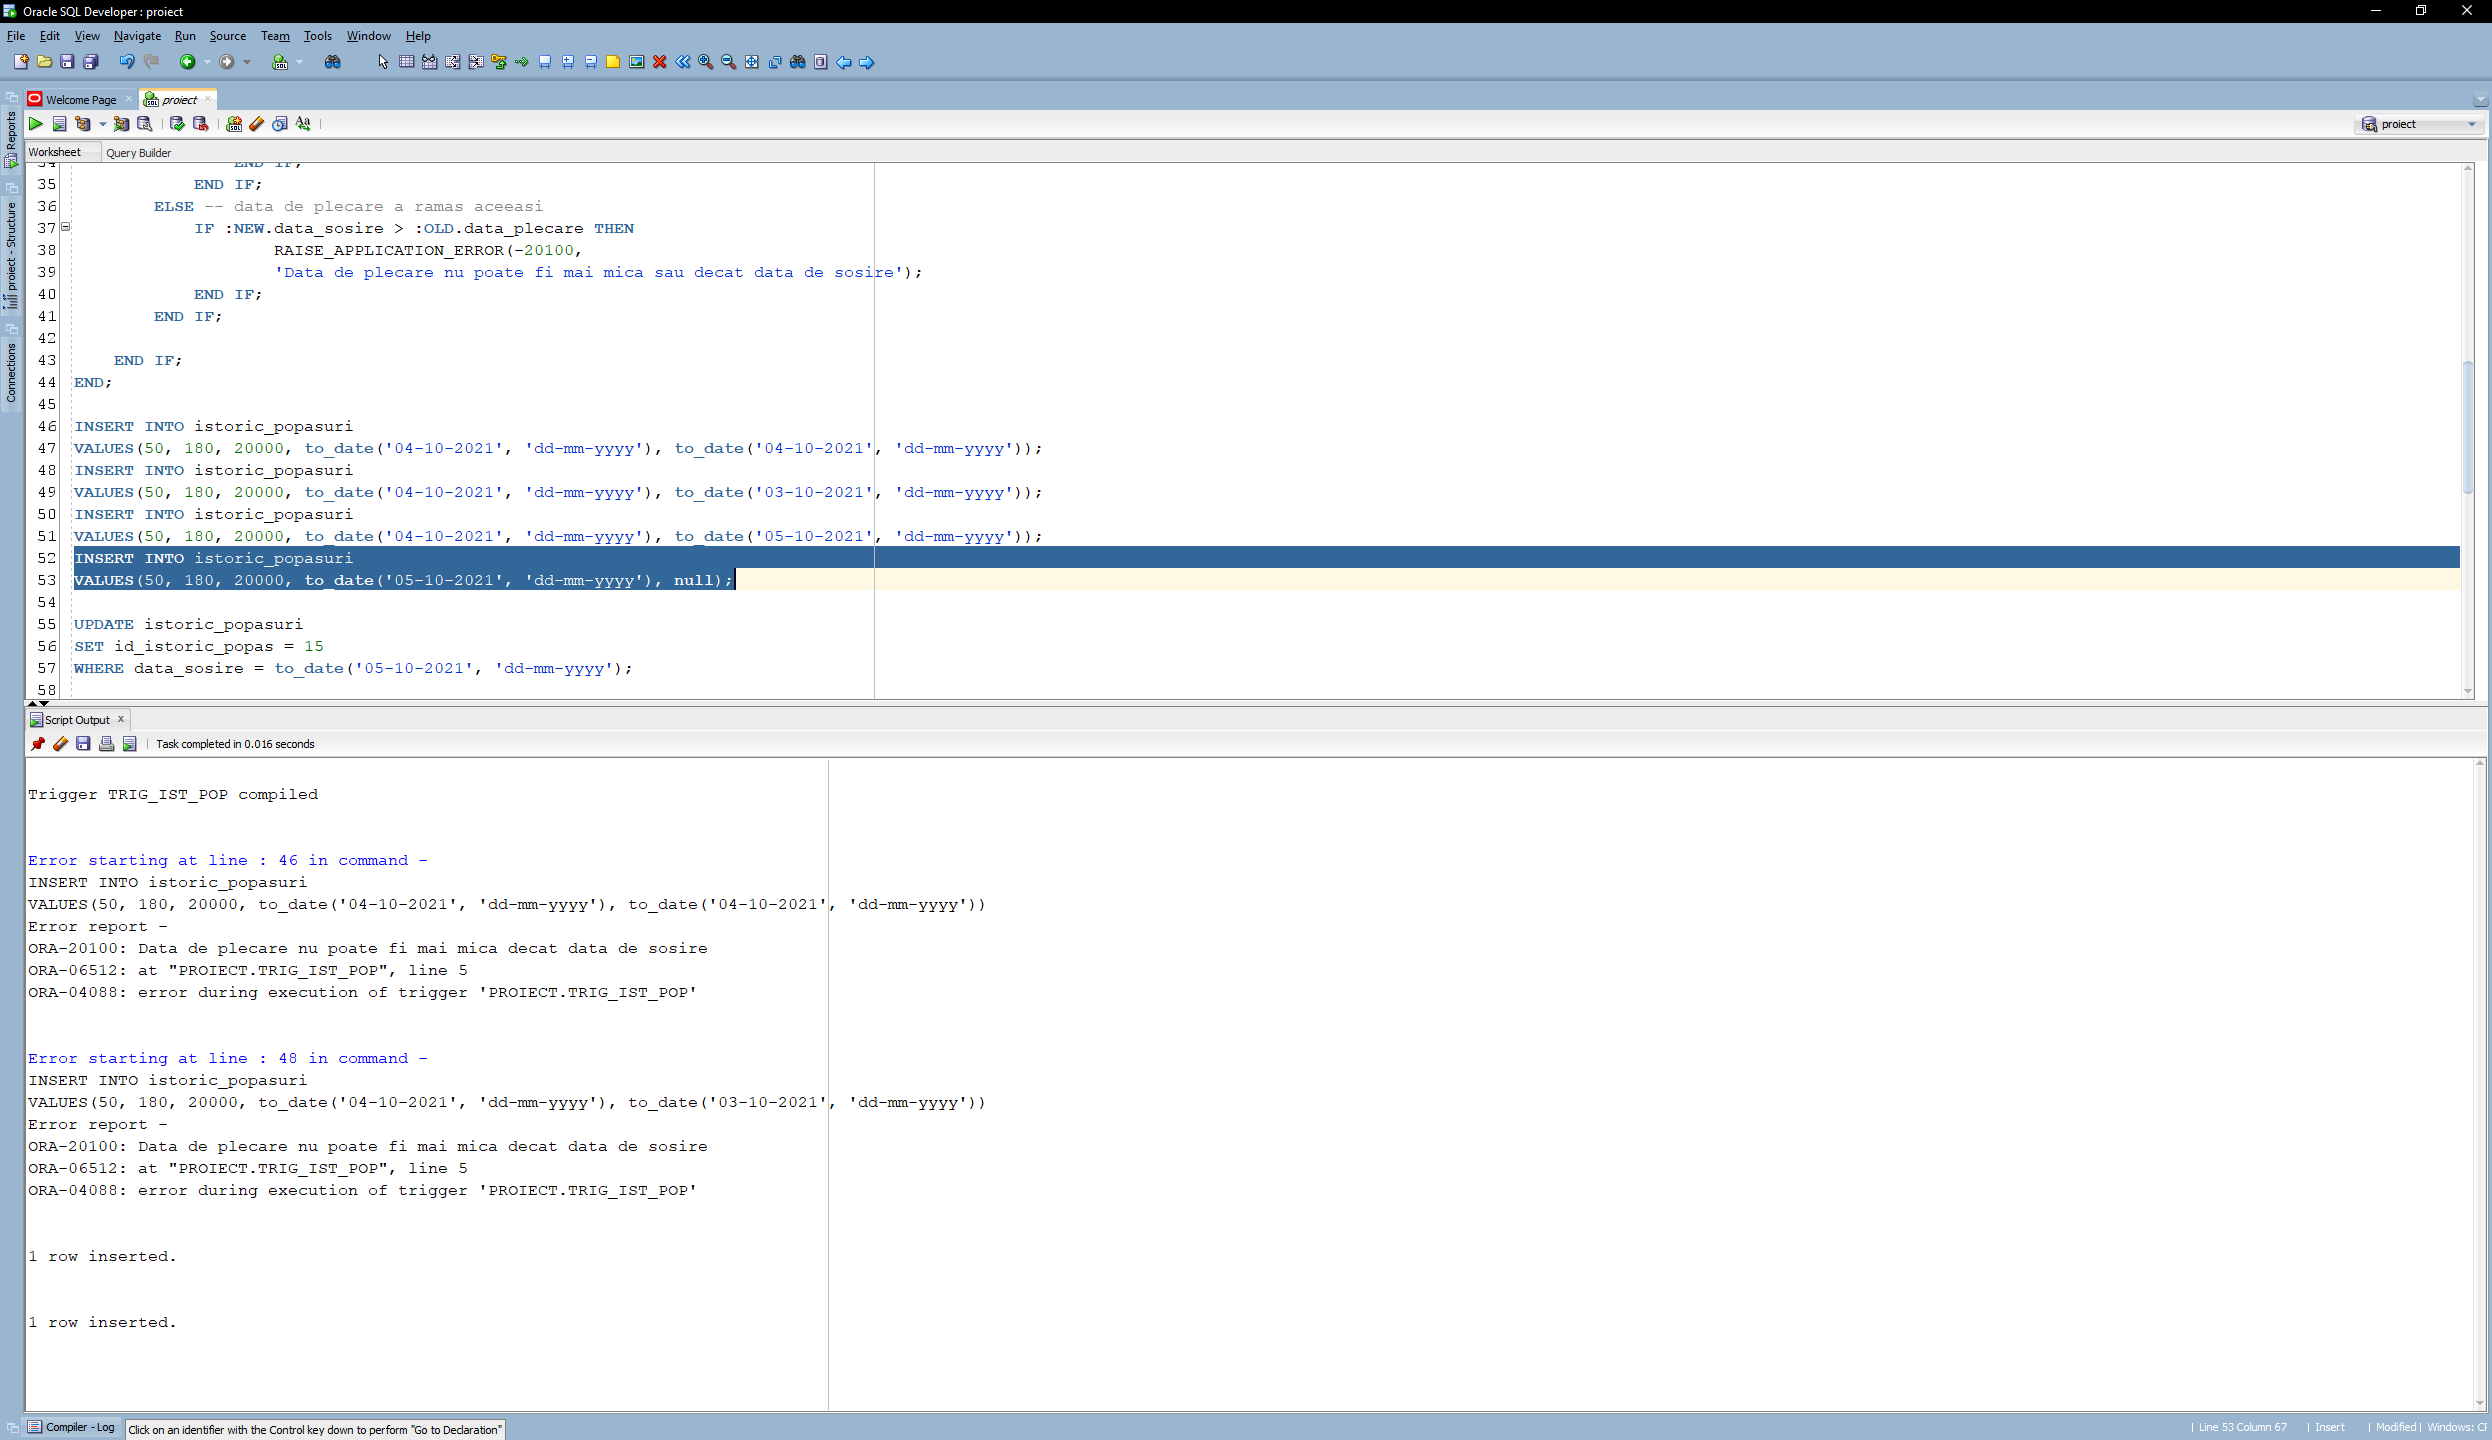
\includegraphics[width=\textwidth]{11_1.png}

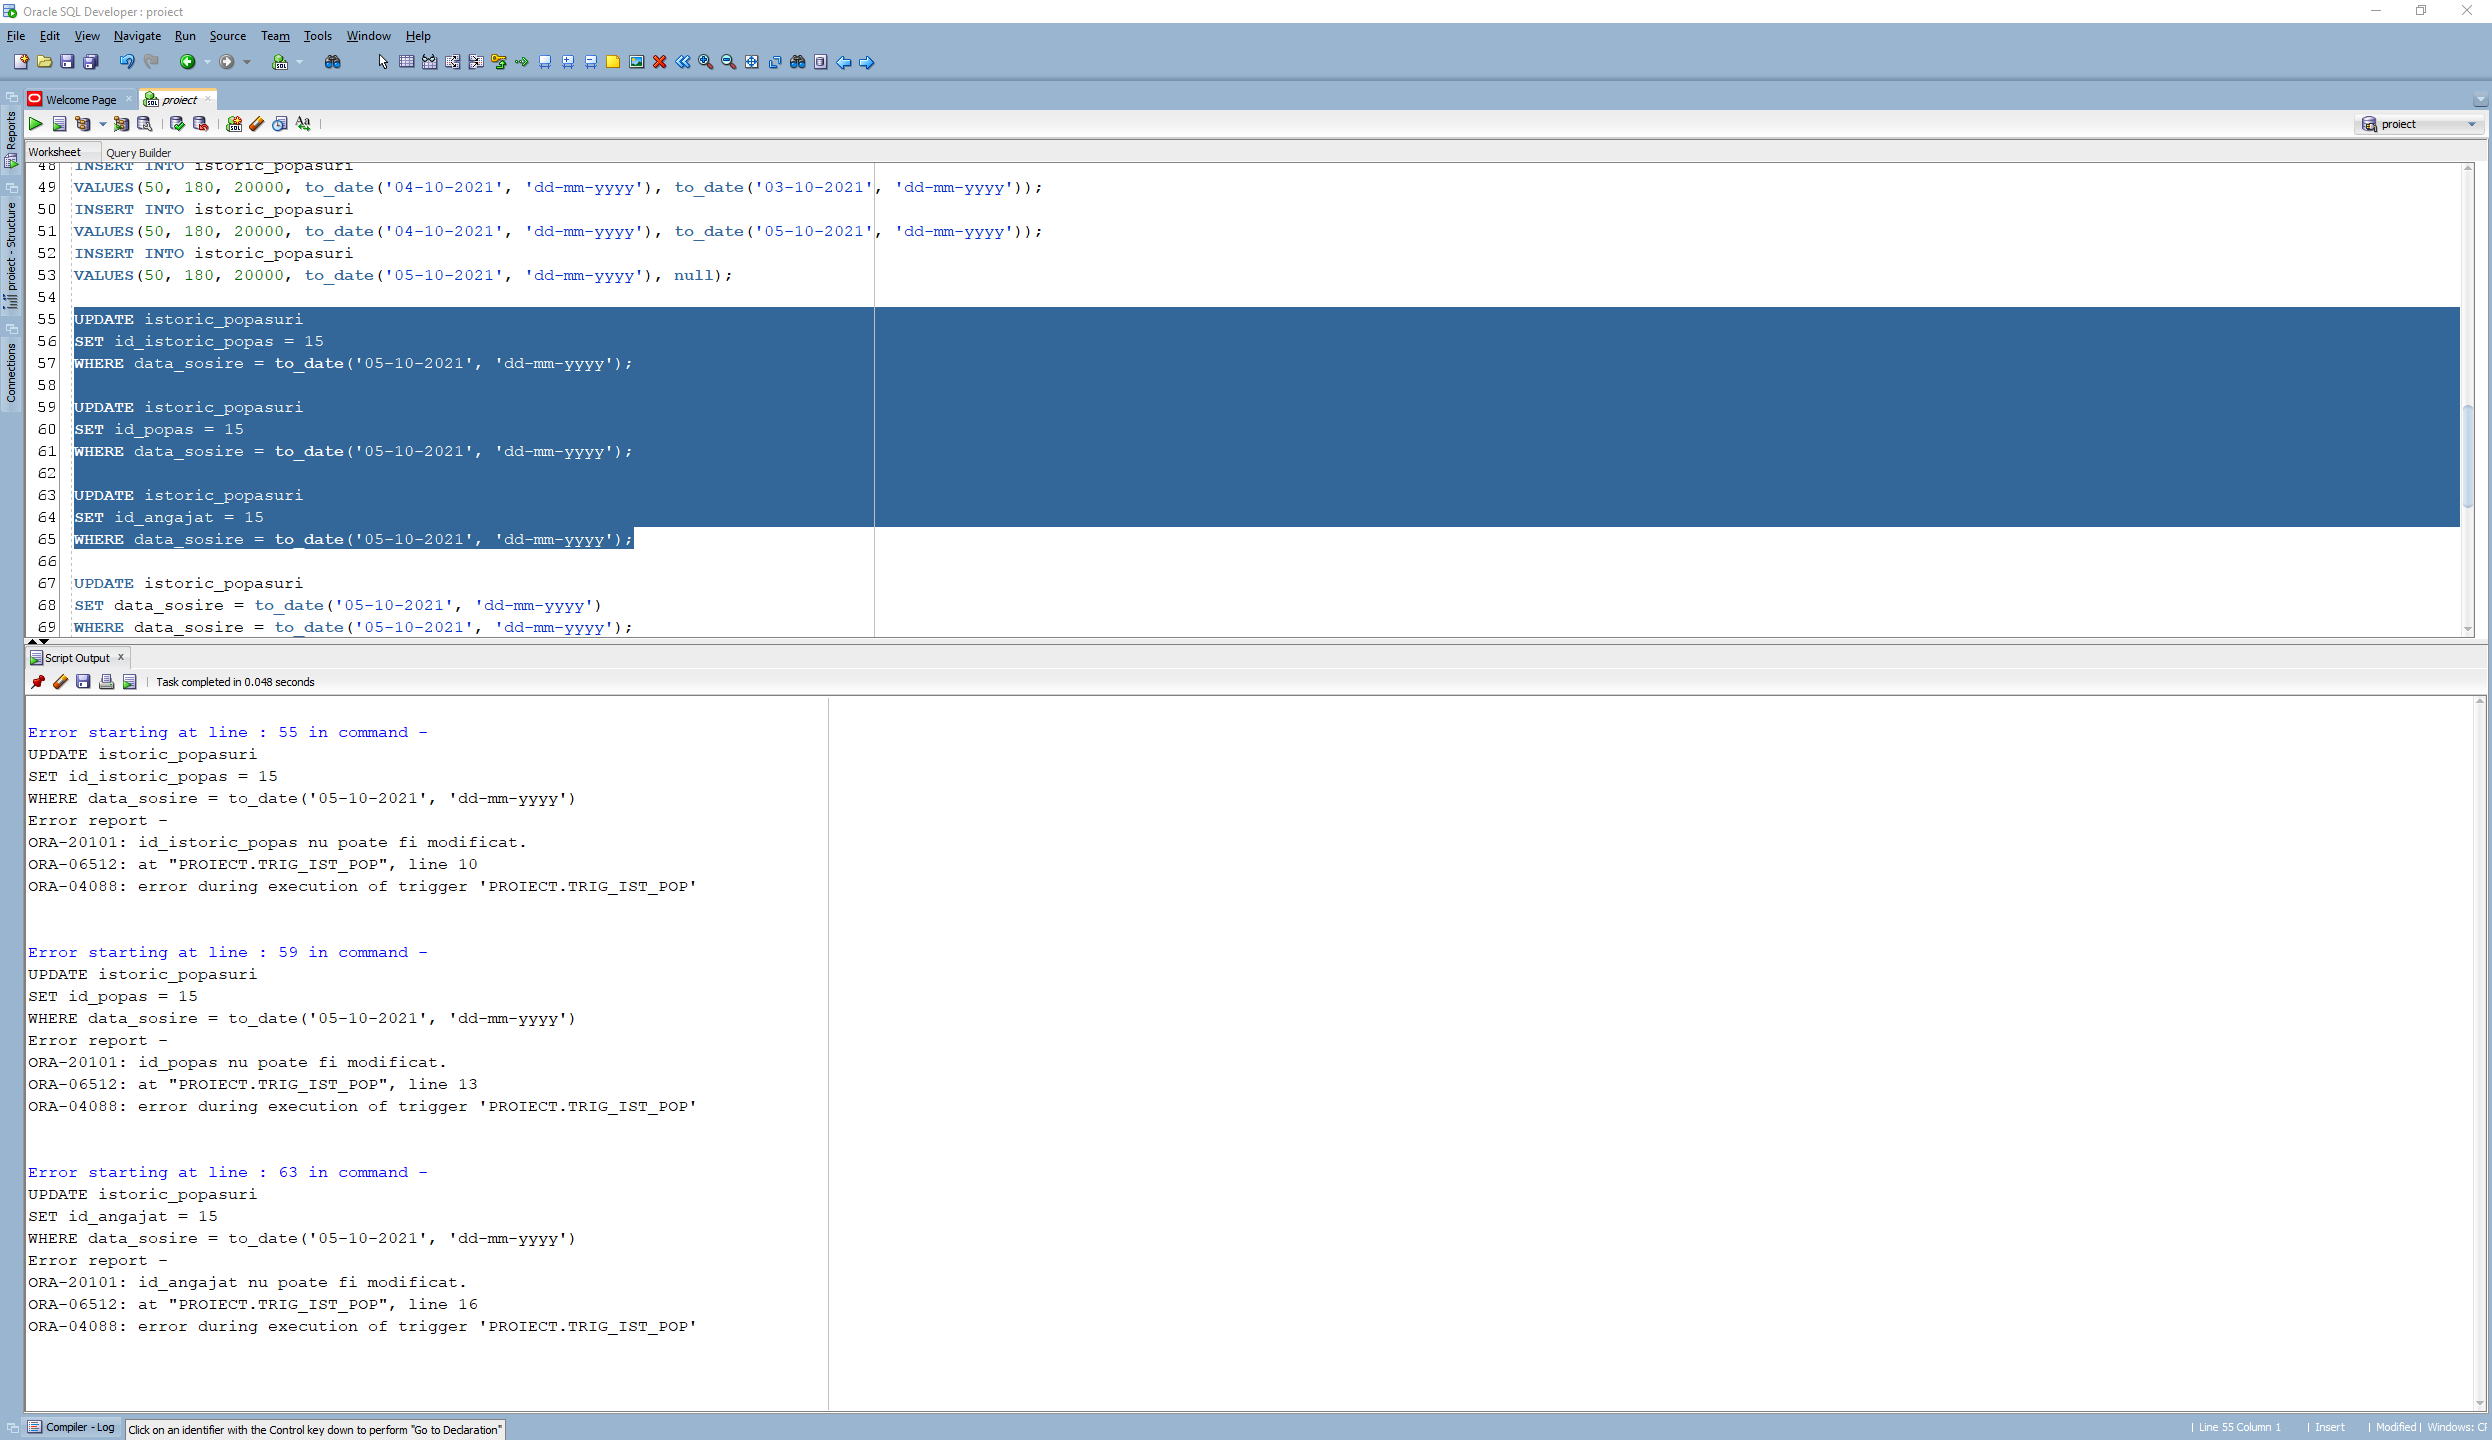
\includegraphics[width=\textwidth]{11_2.png}

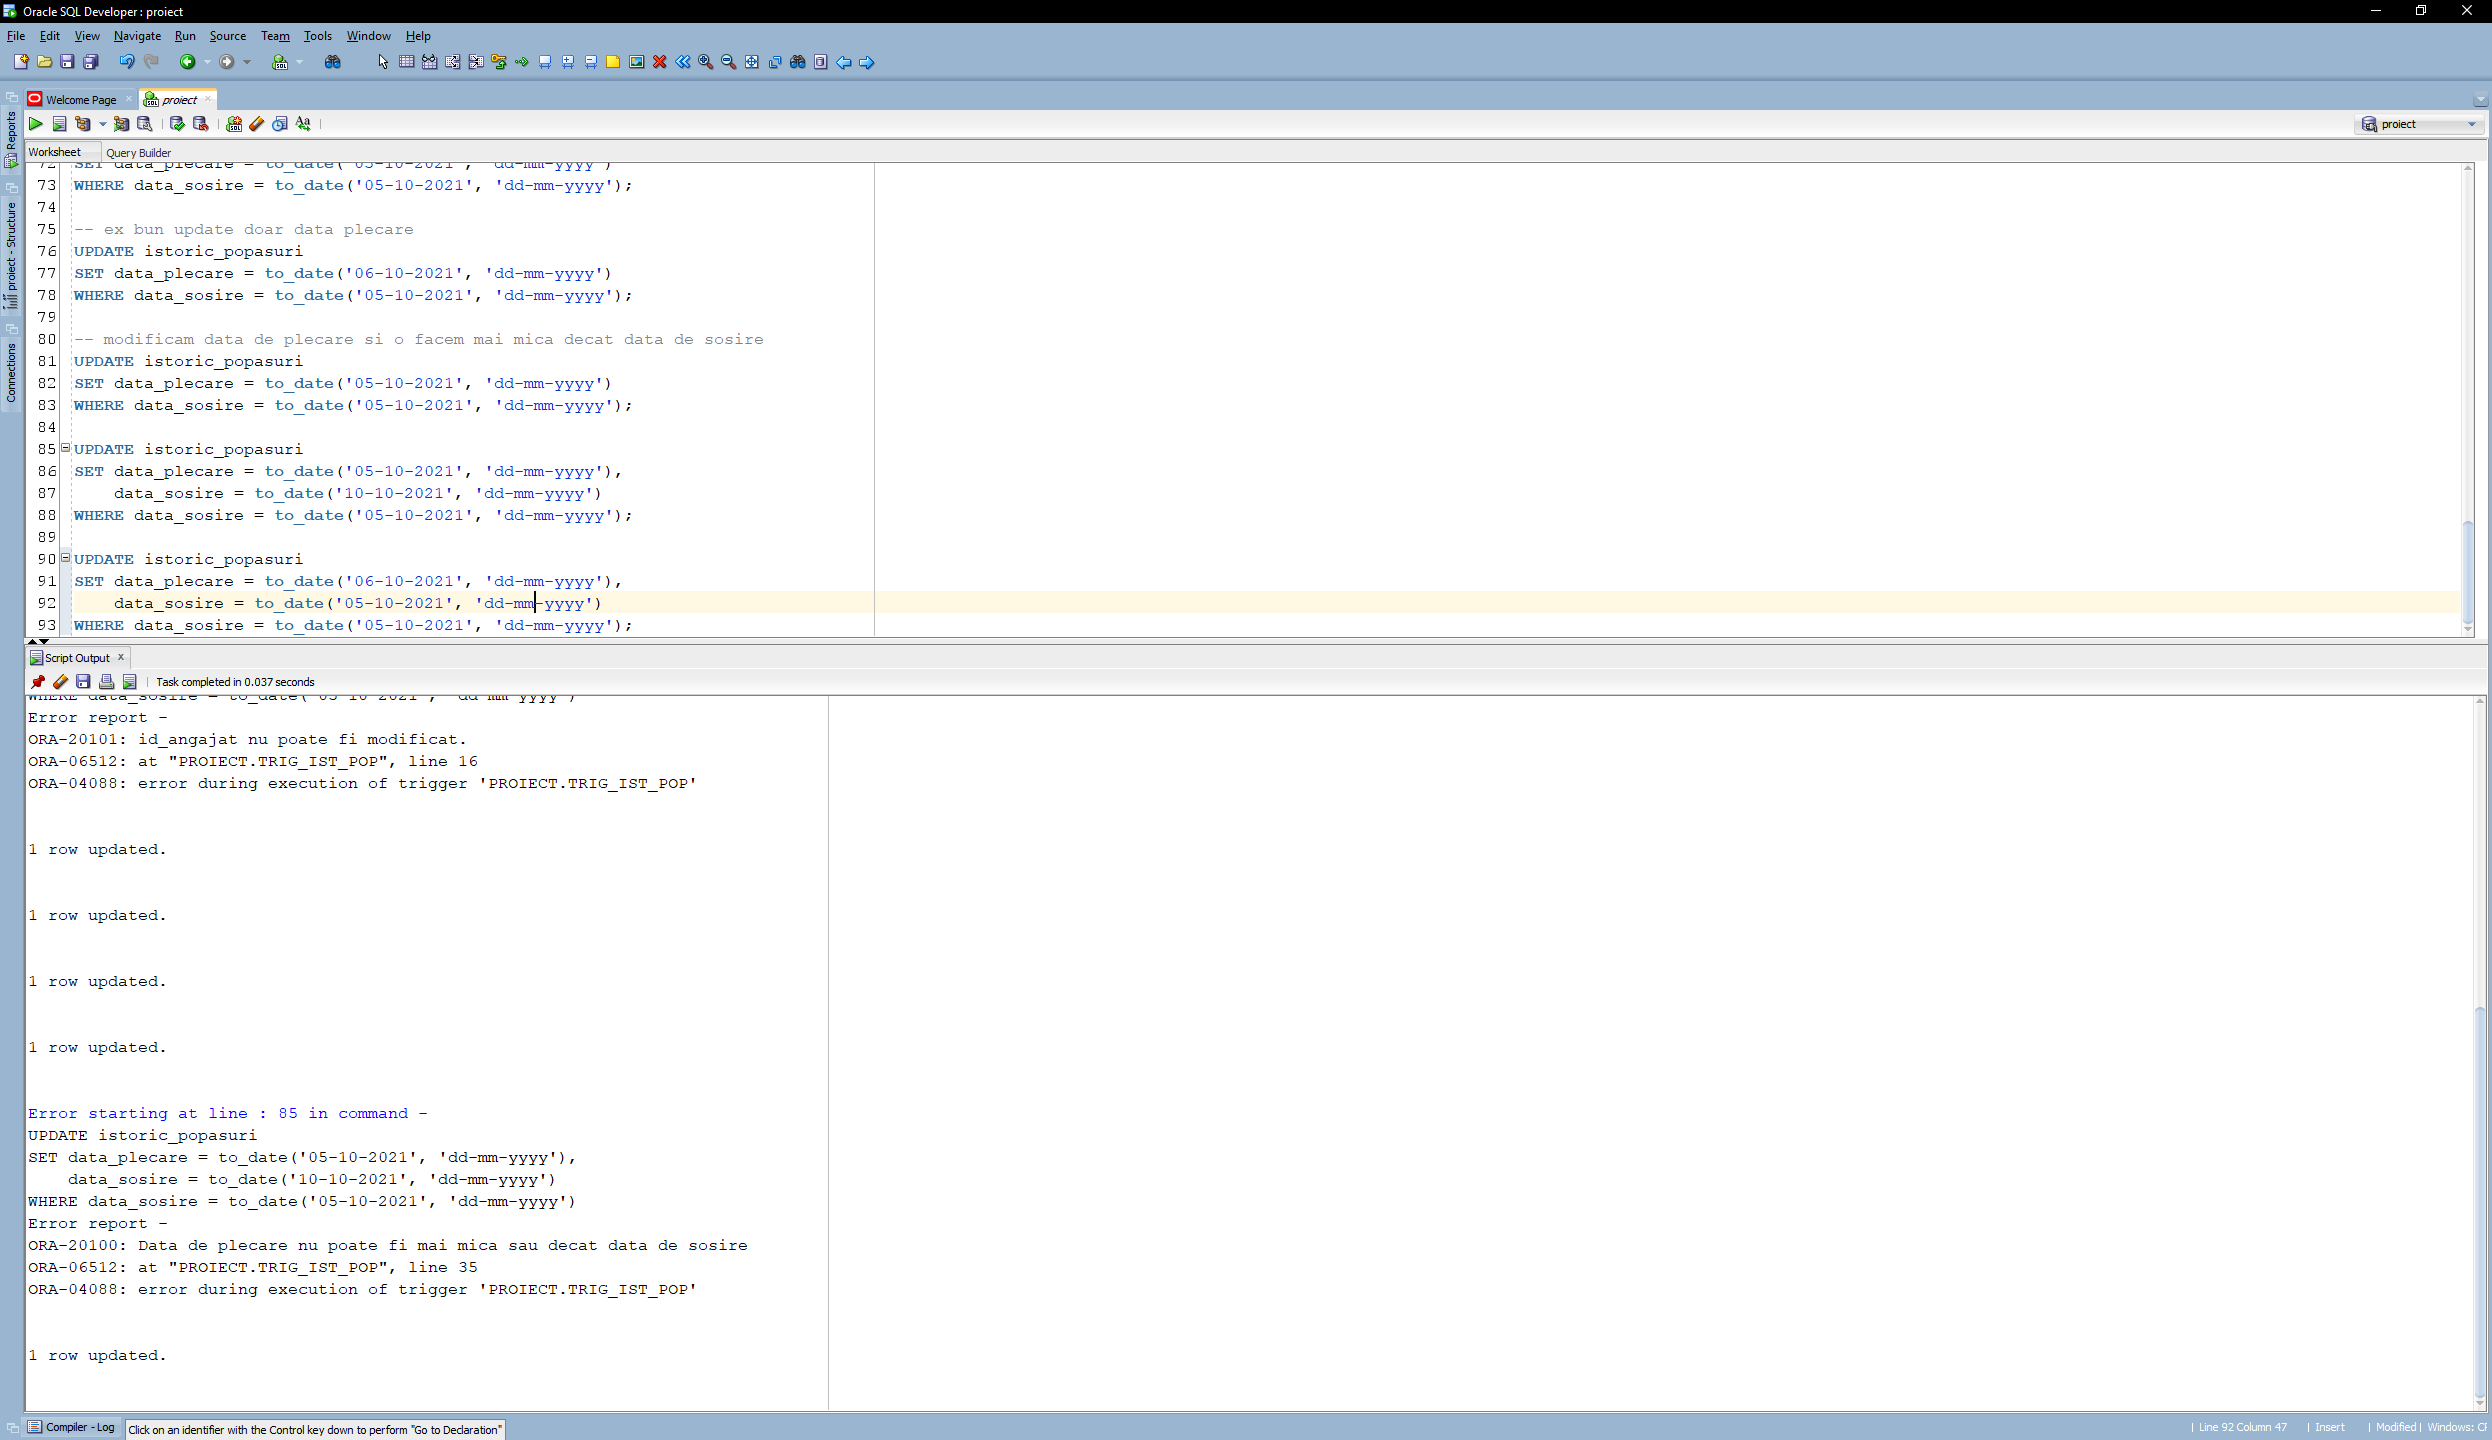
\includegraphics[width=\textwidth]{11_3.png}

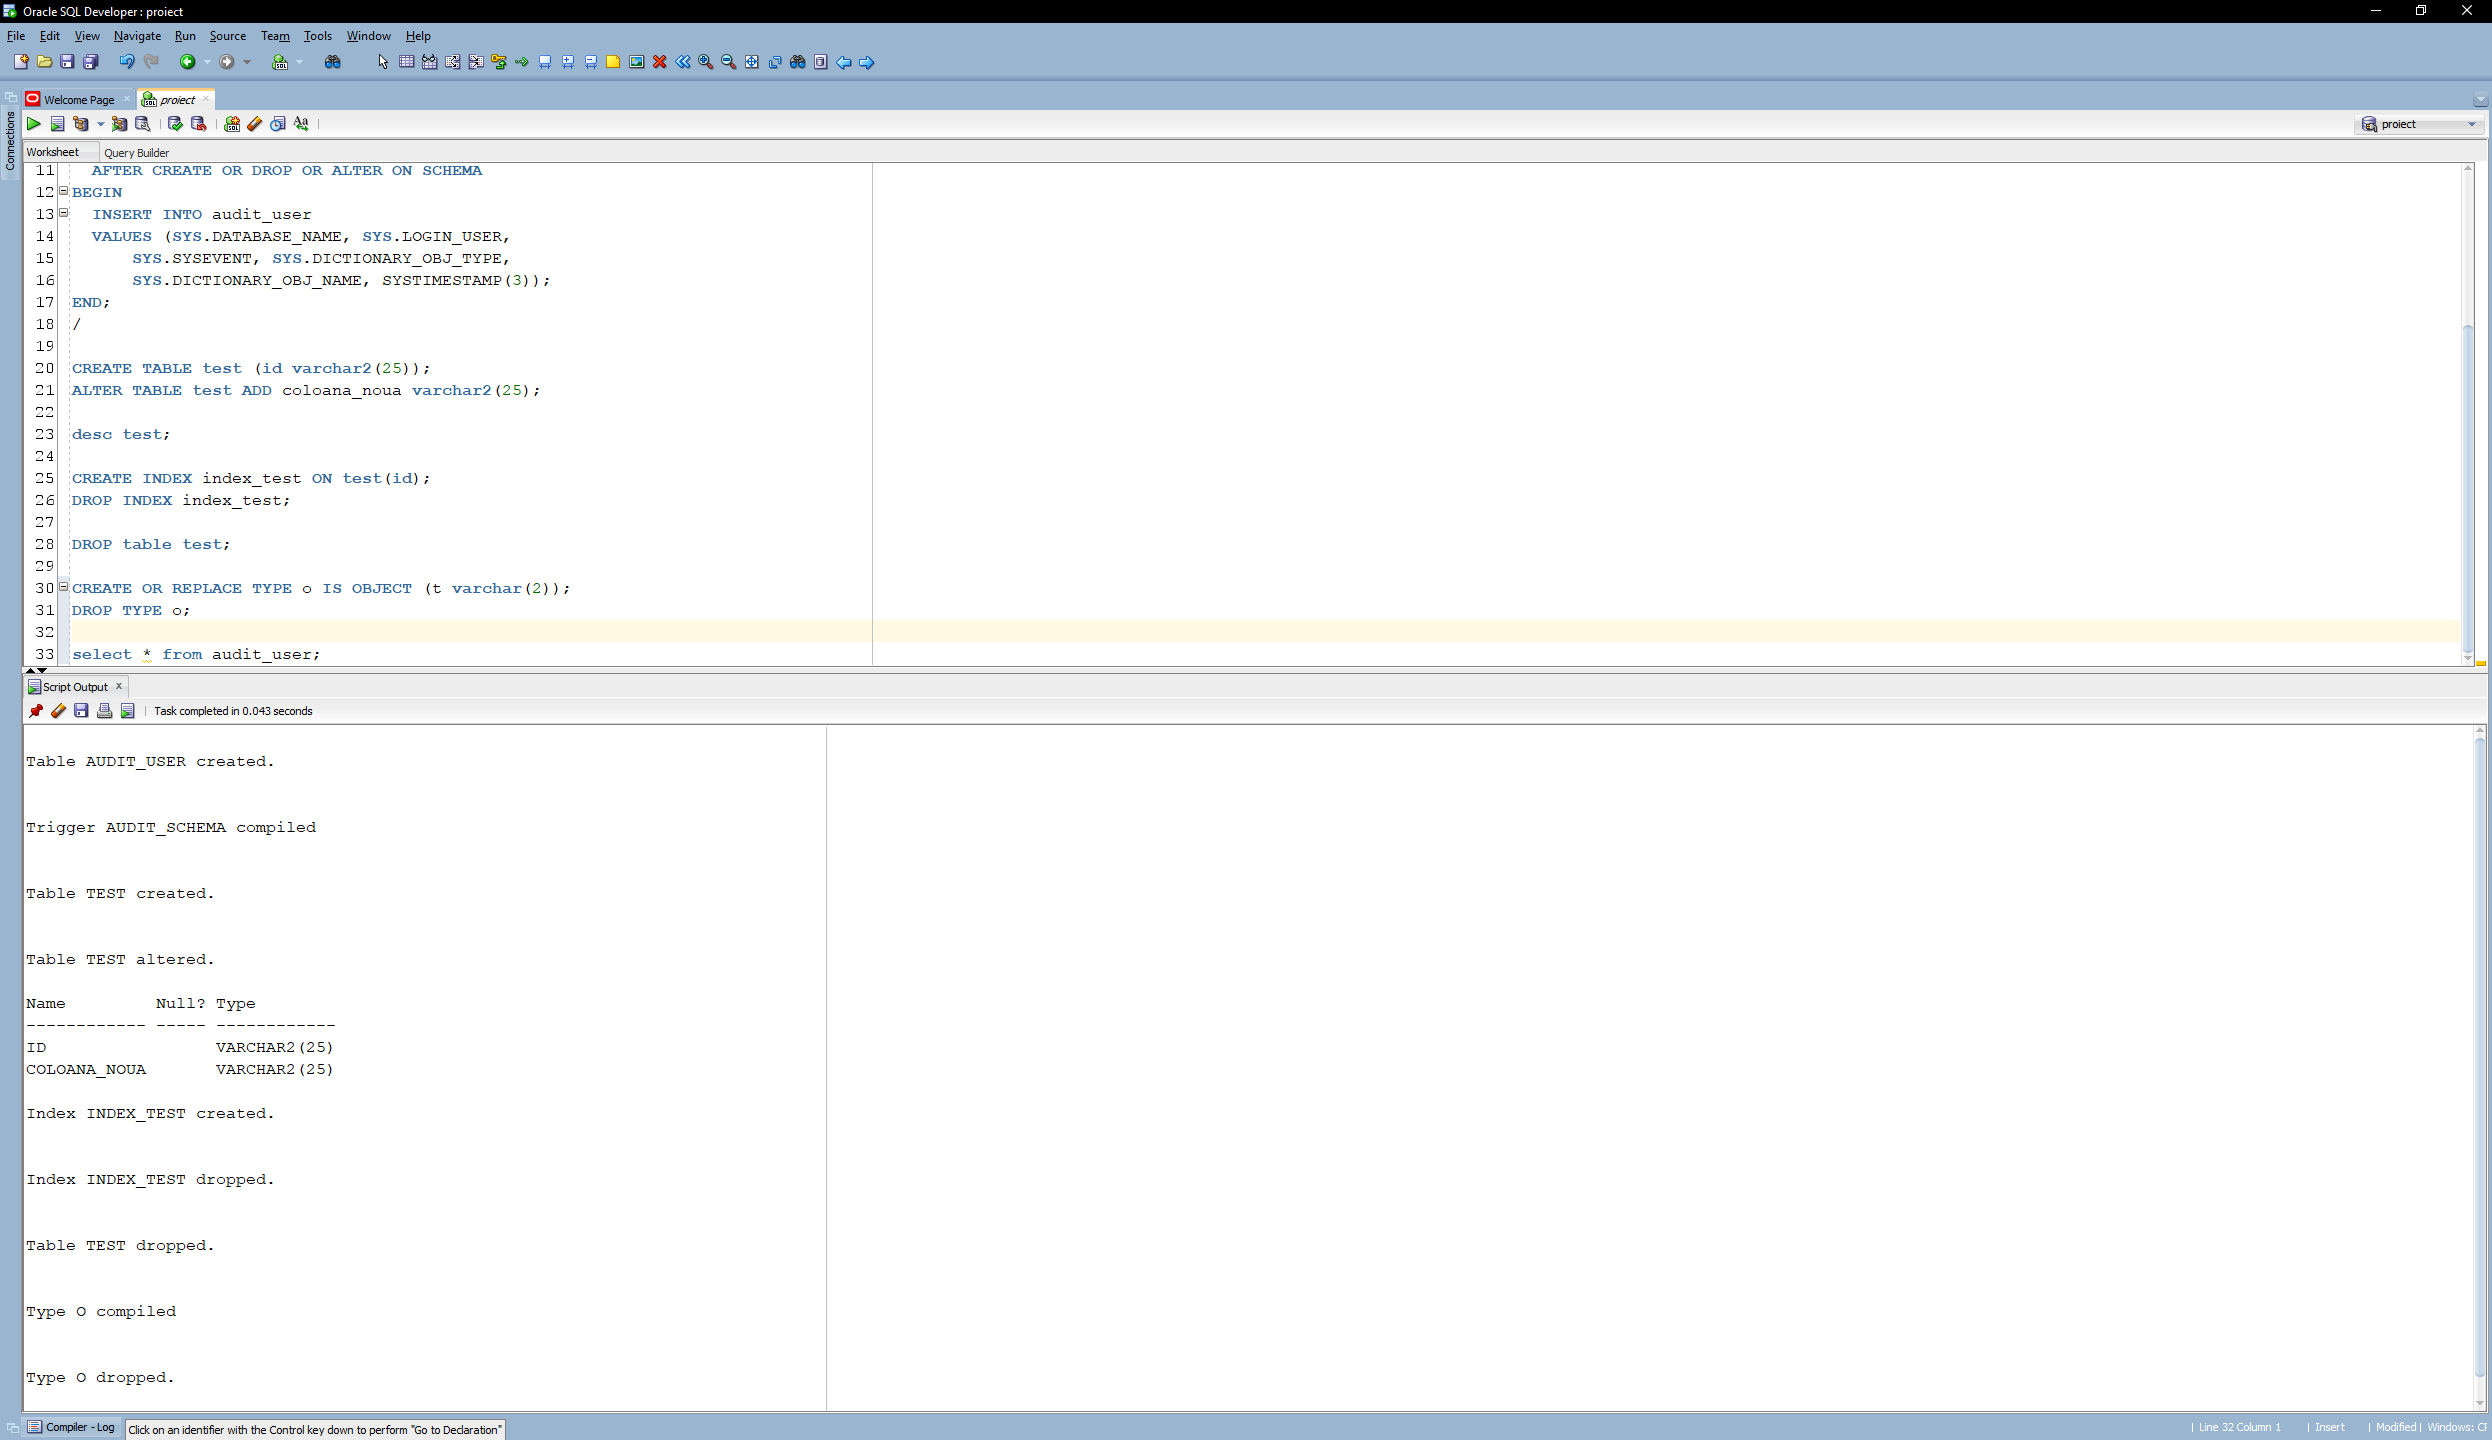
\includegraphics[width=\textwidth]{12_1.png}

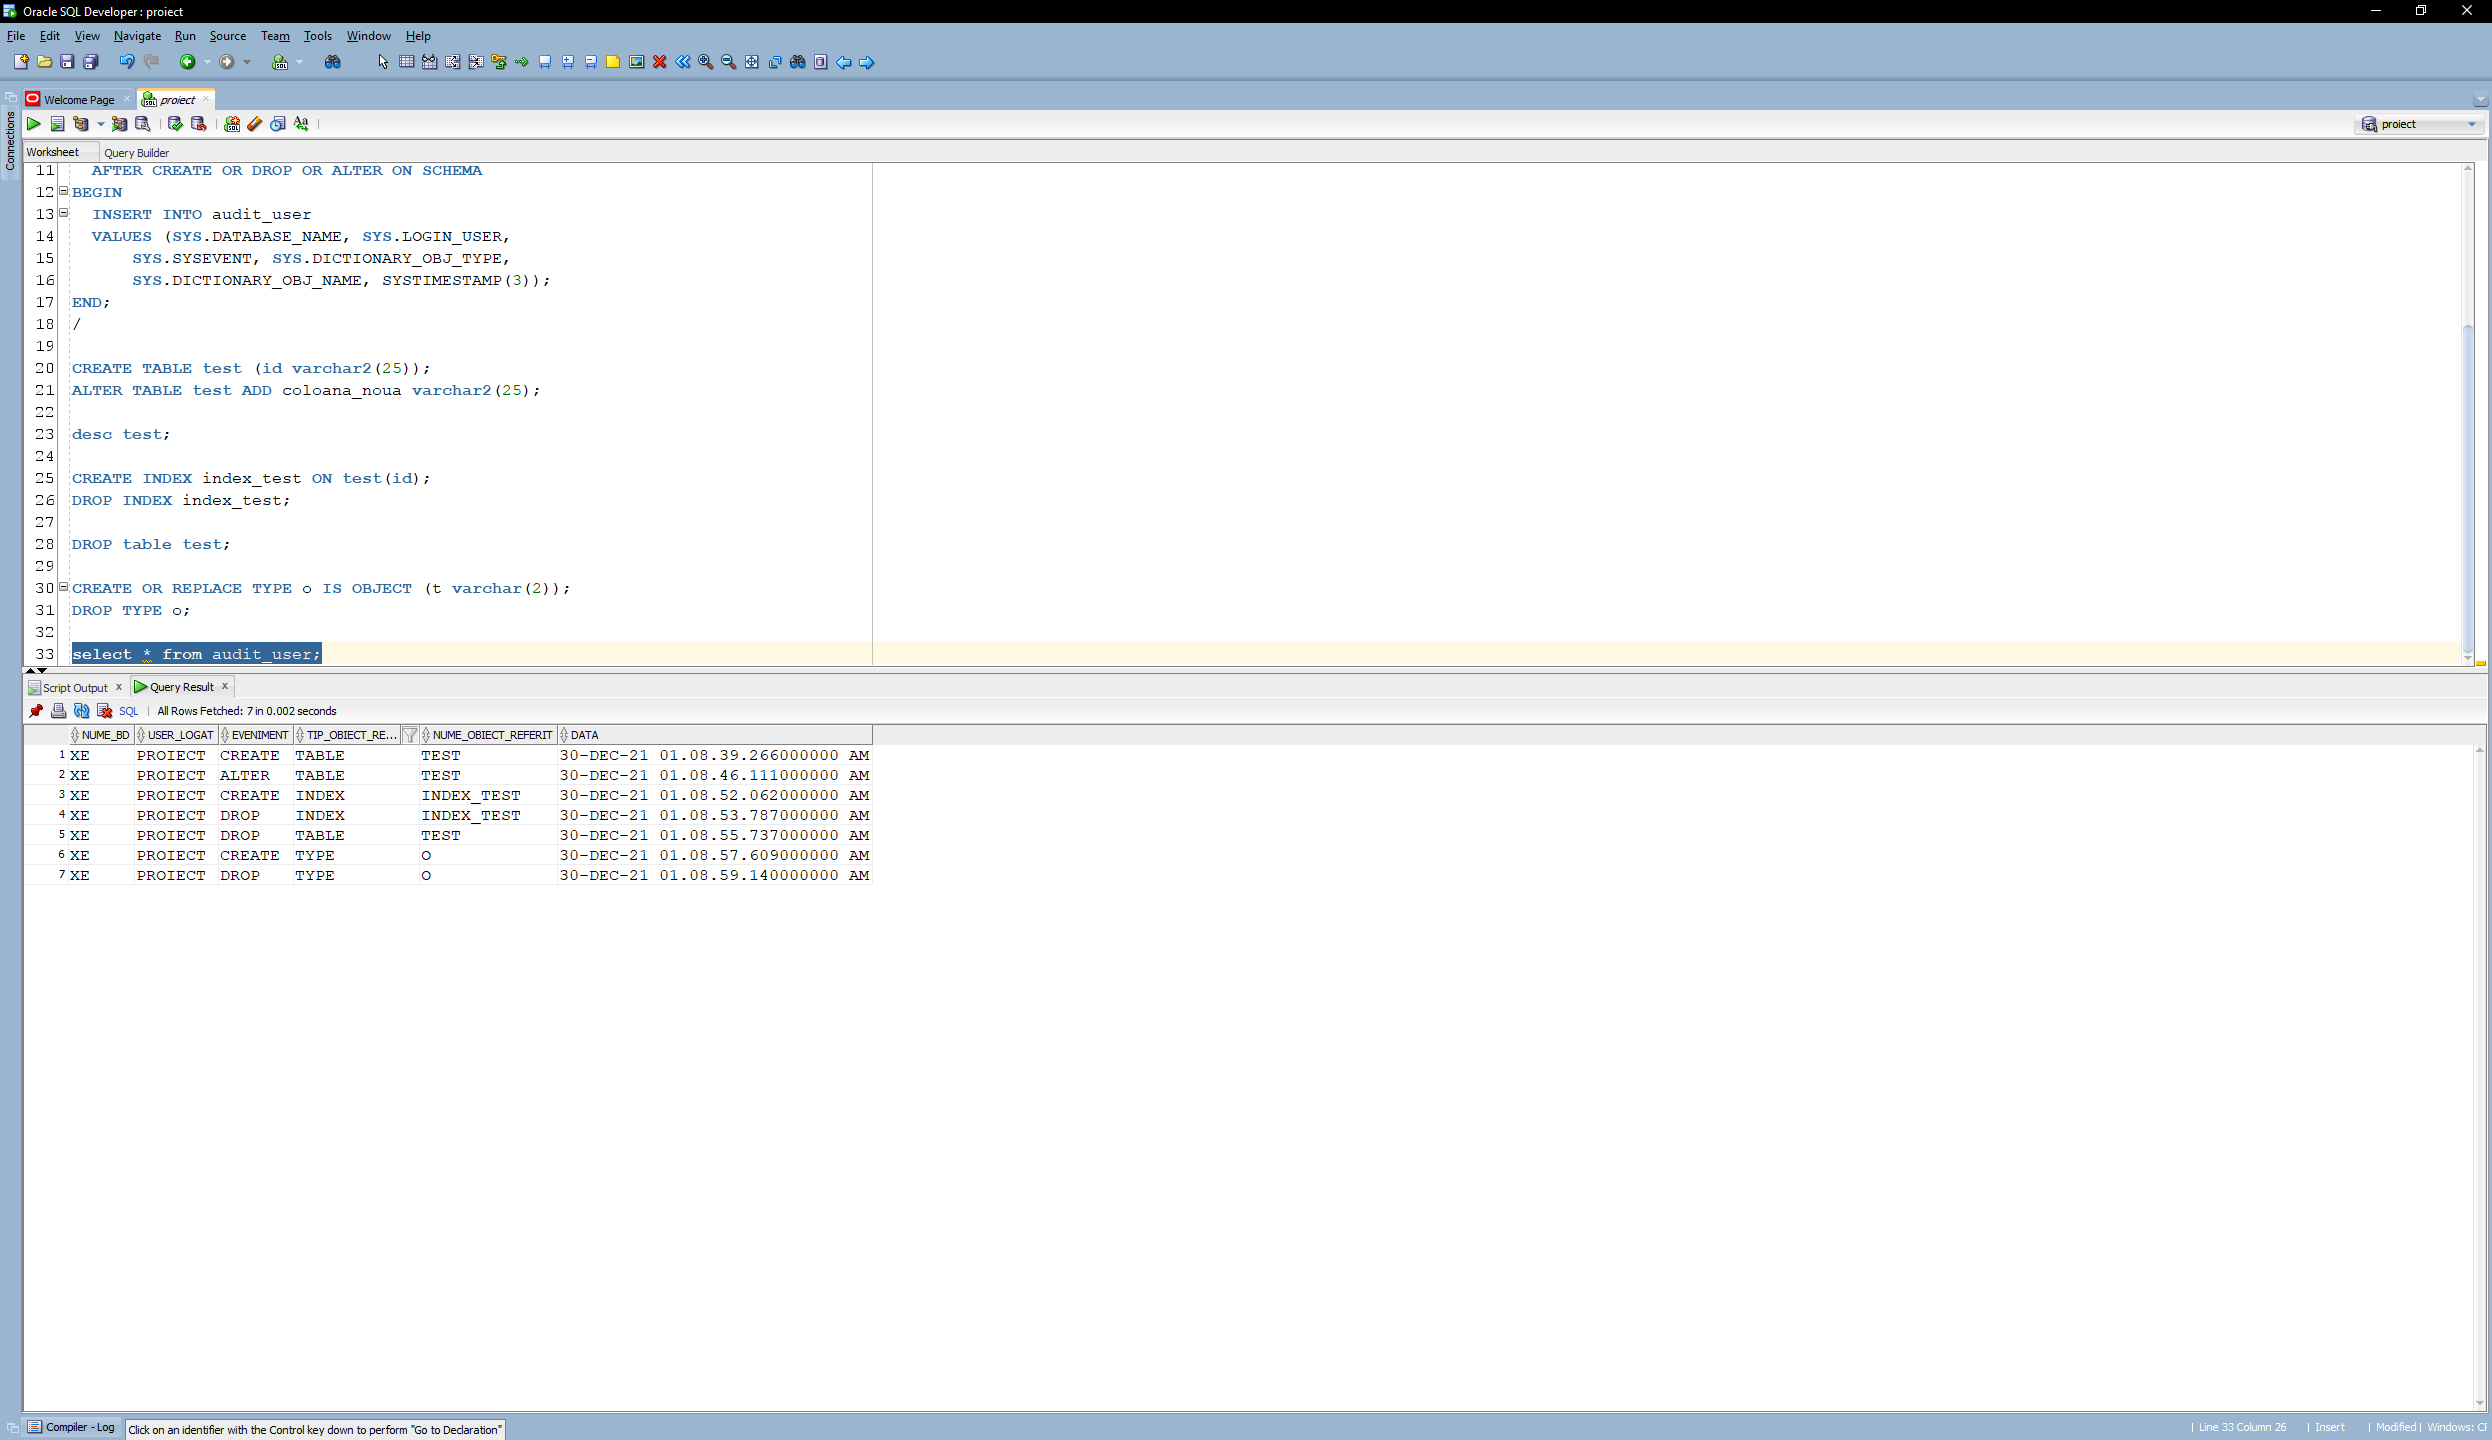
\includegraphics[width=\textwidth]{12_2.png}

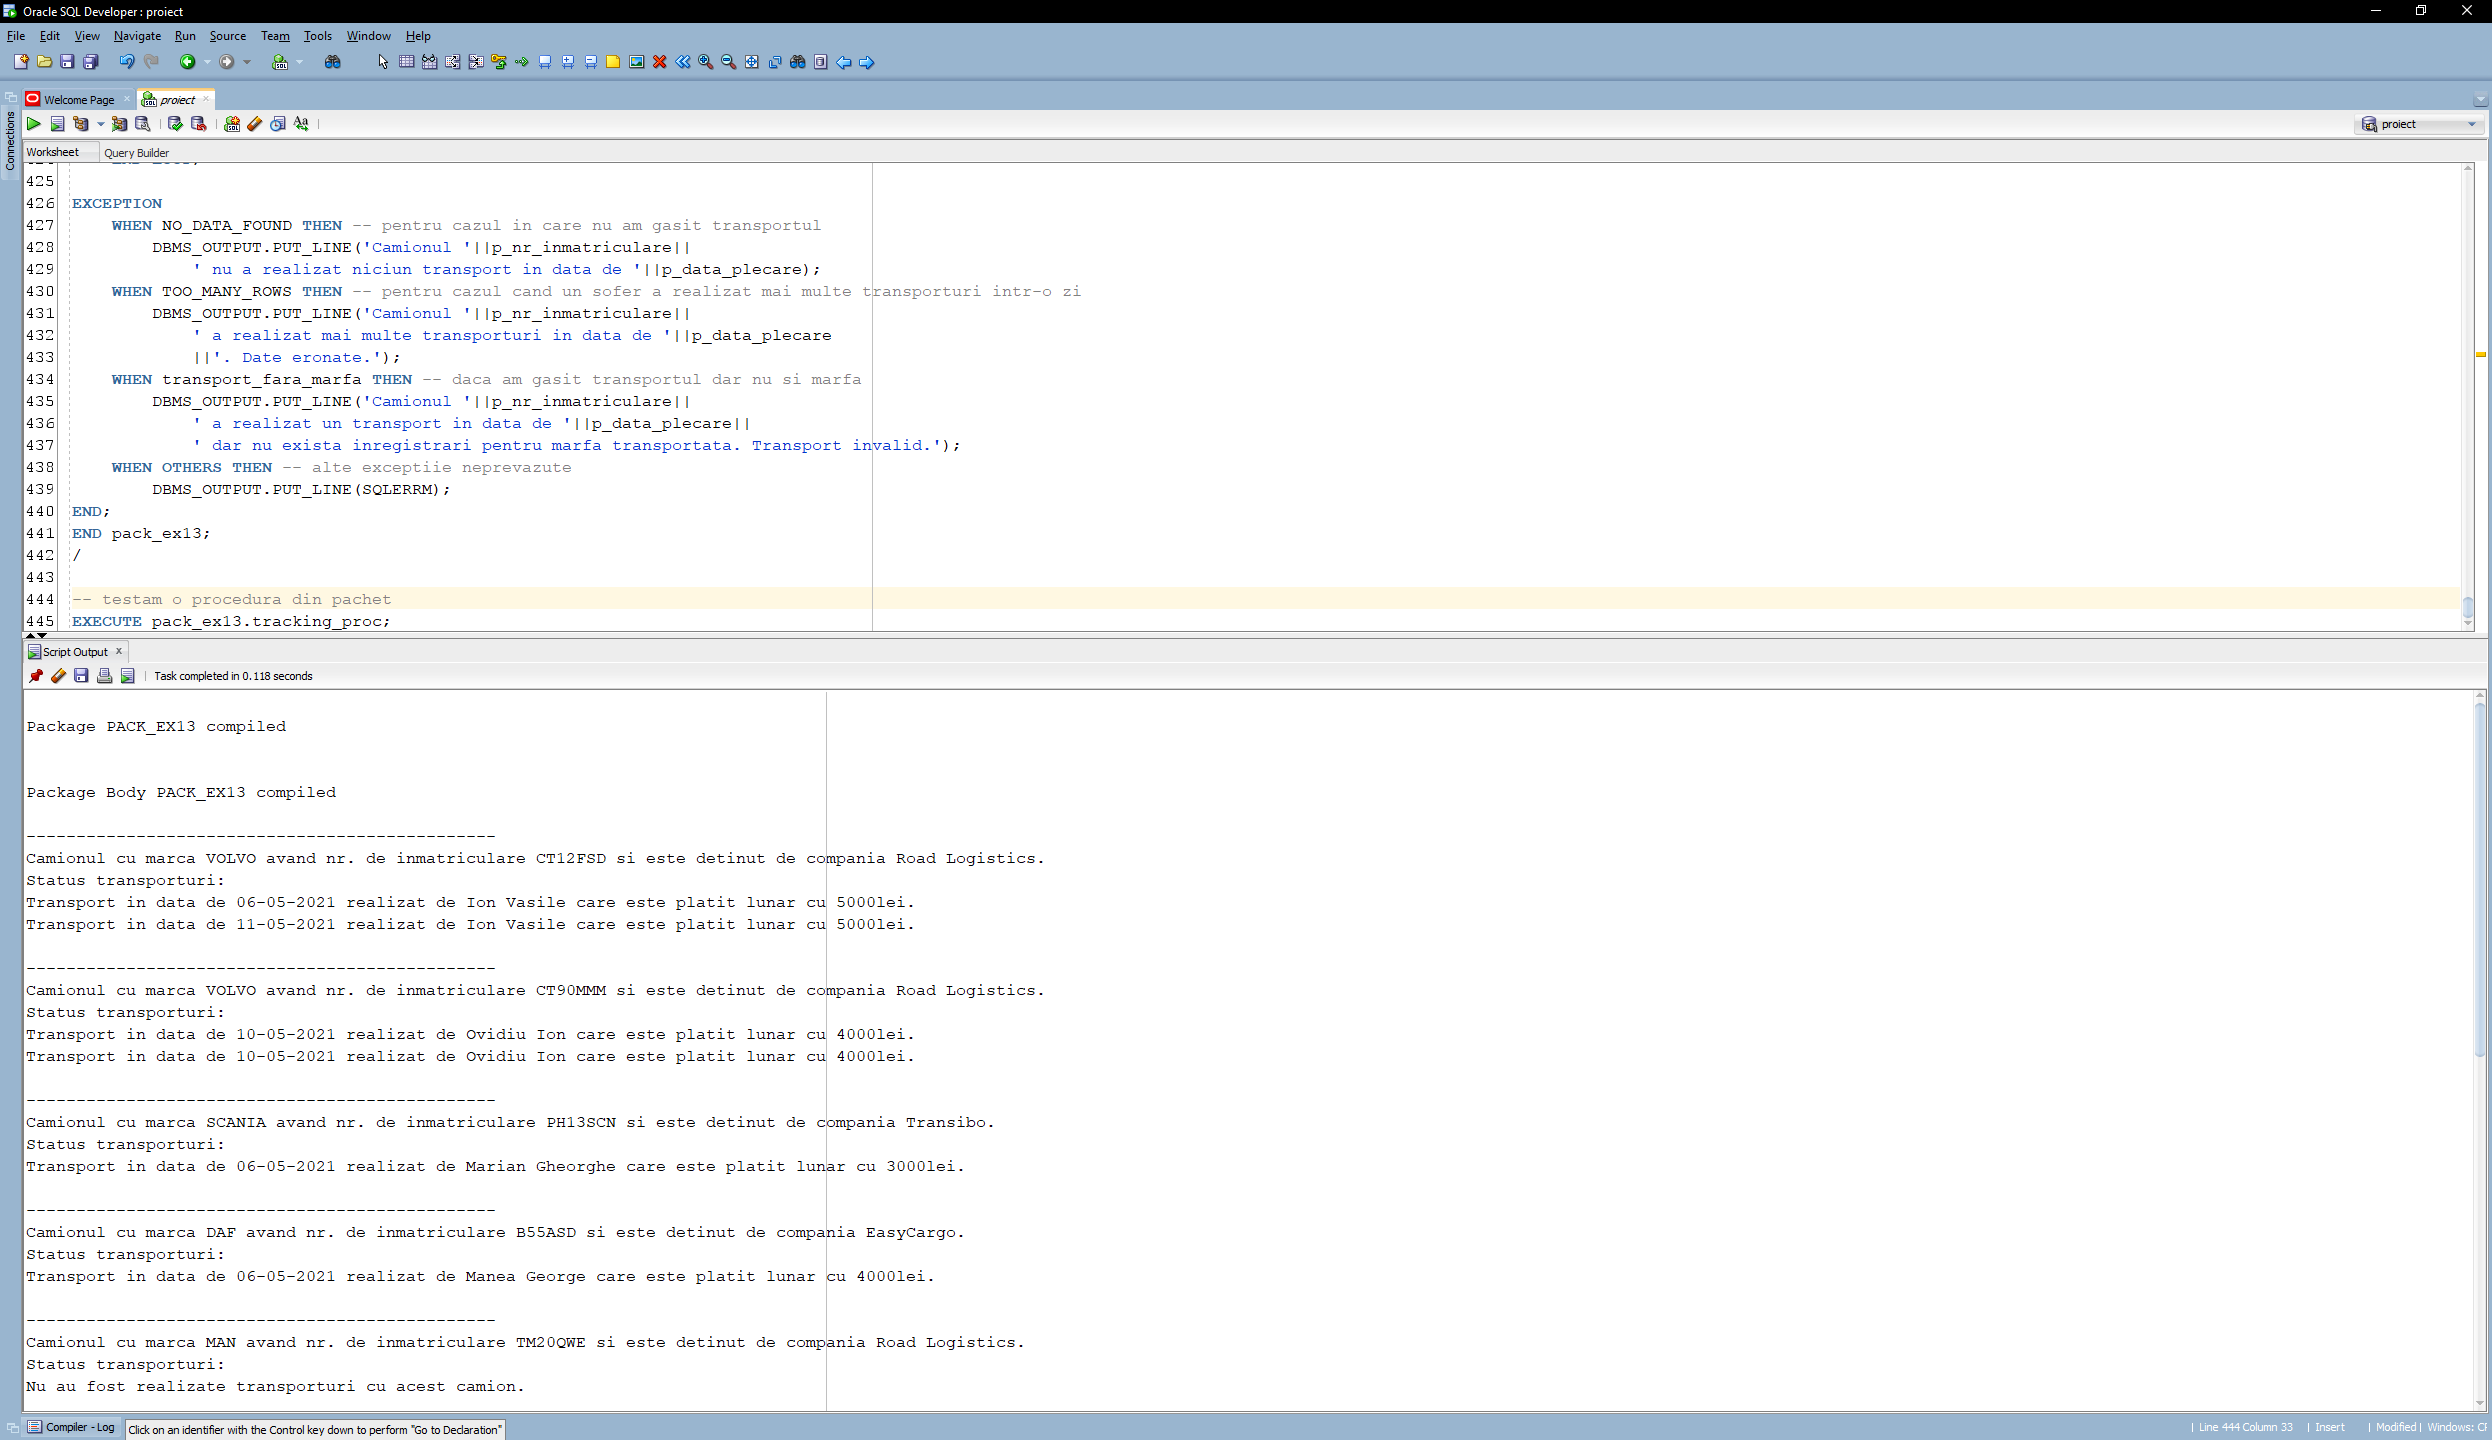
\includegraphics[width=\textwidth]{13.png}

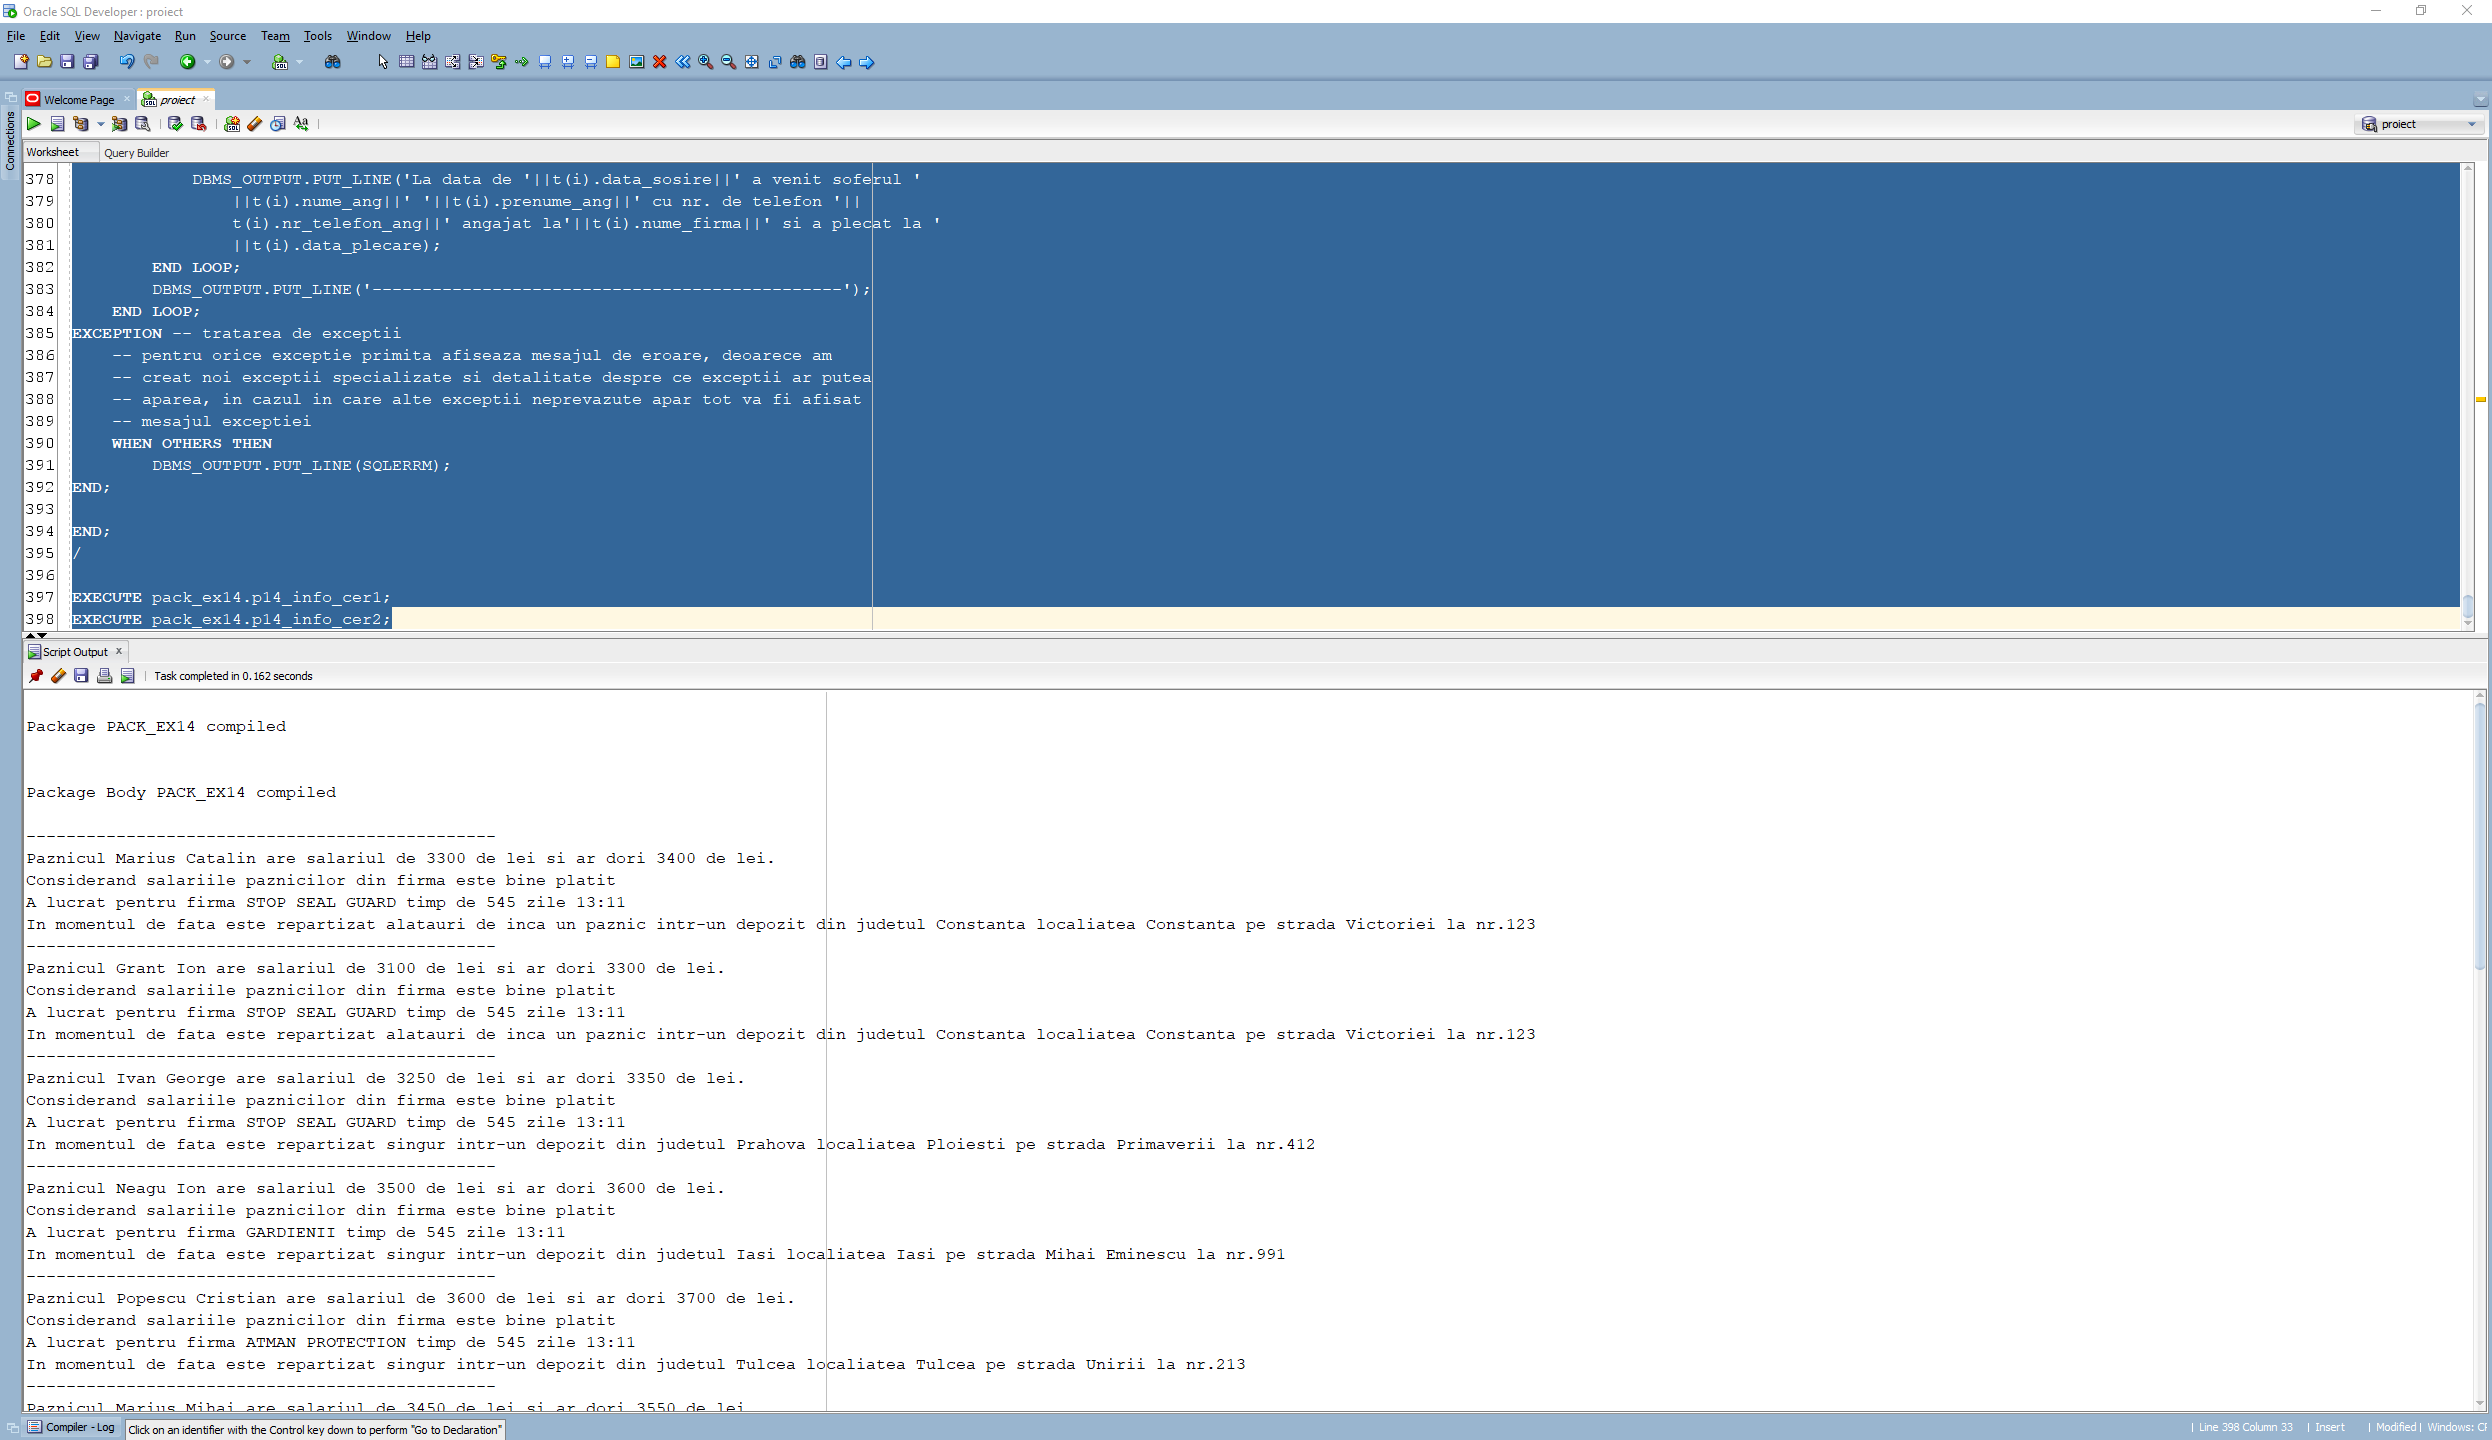
\includegraphics[width=\textwidth]{14_1.png}

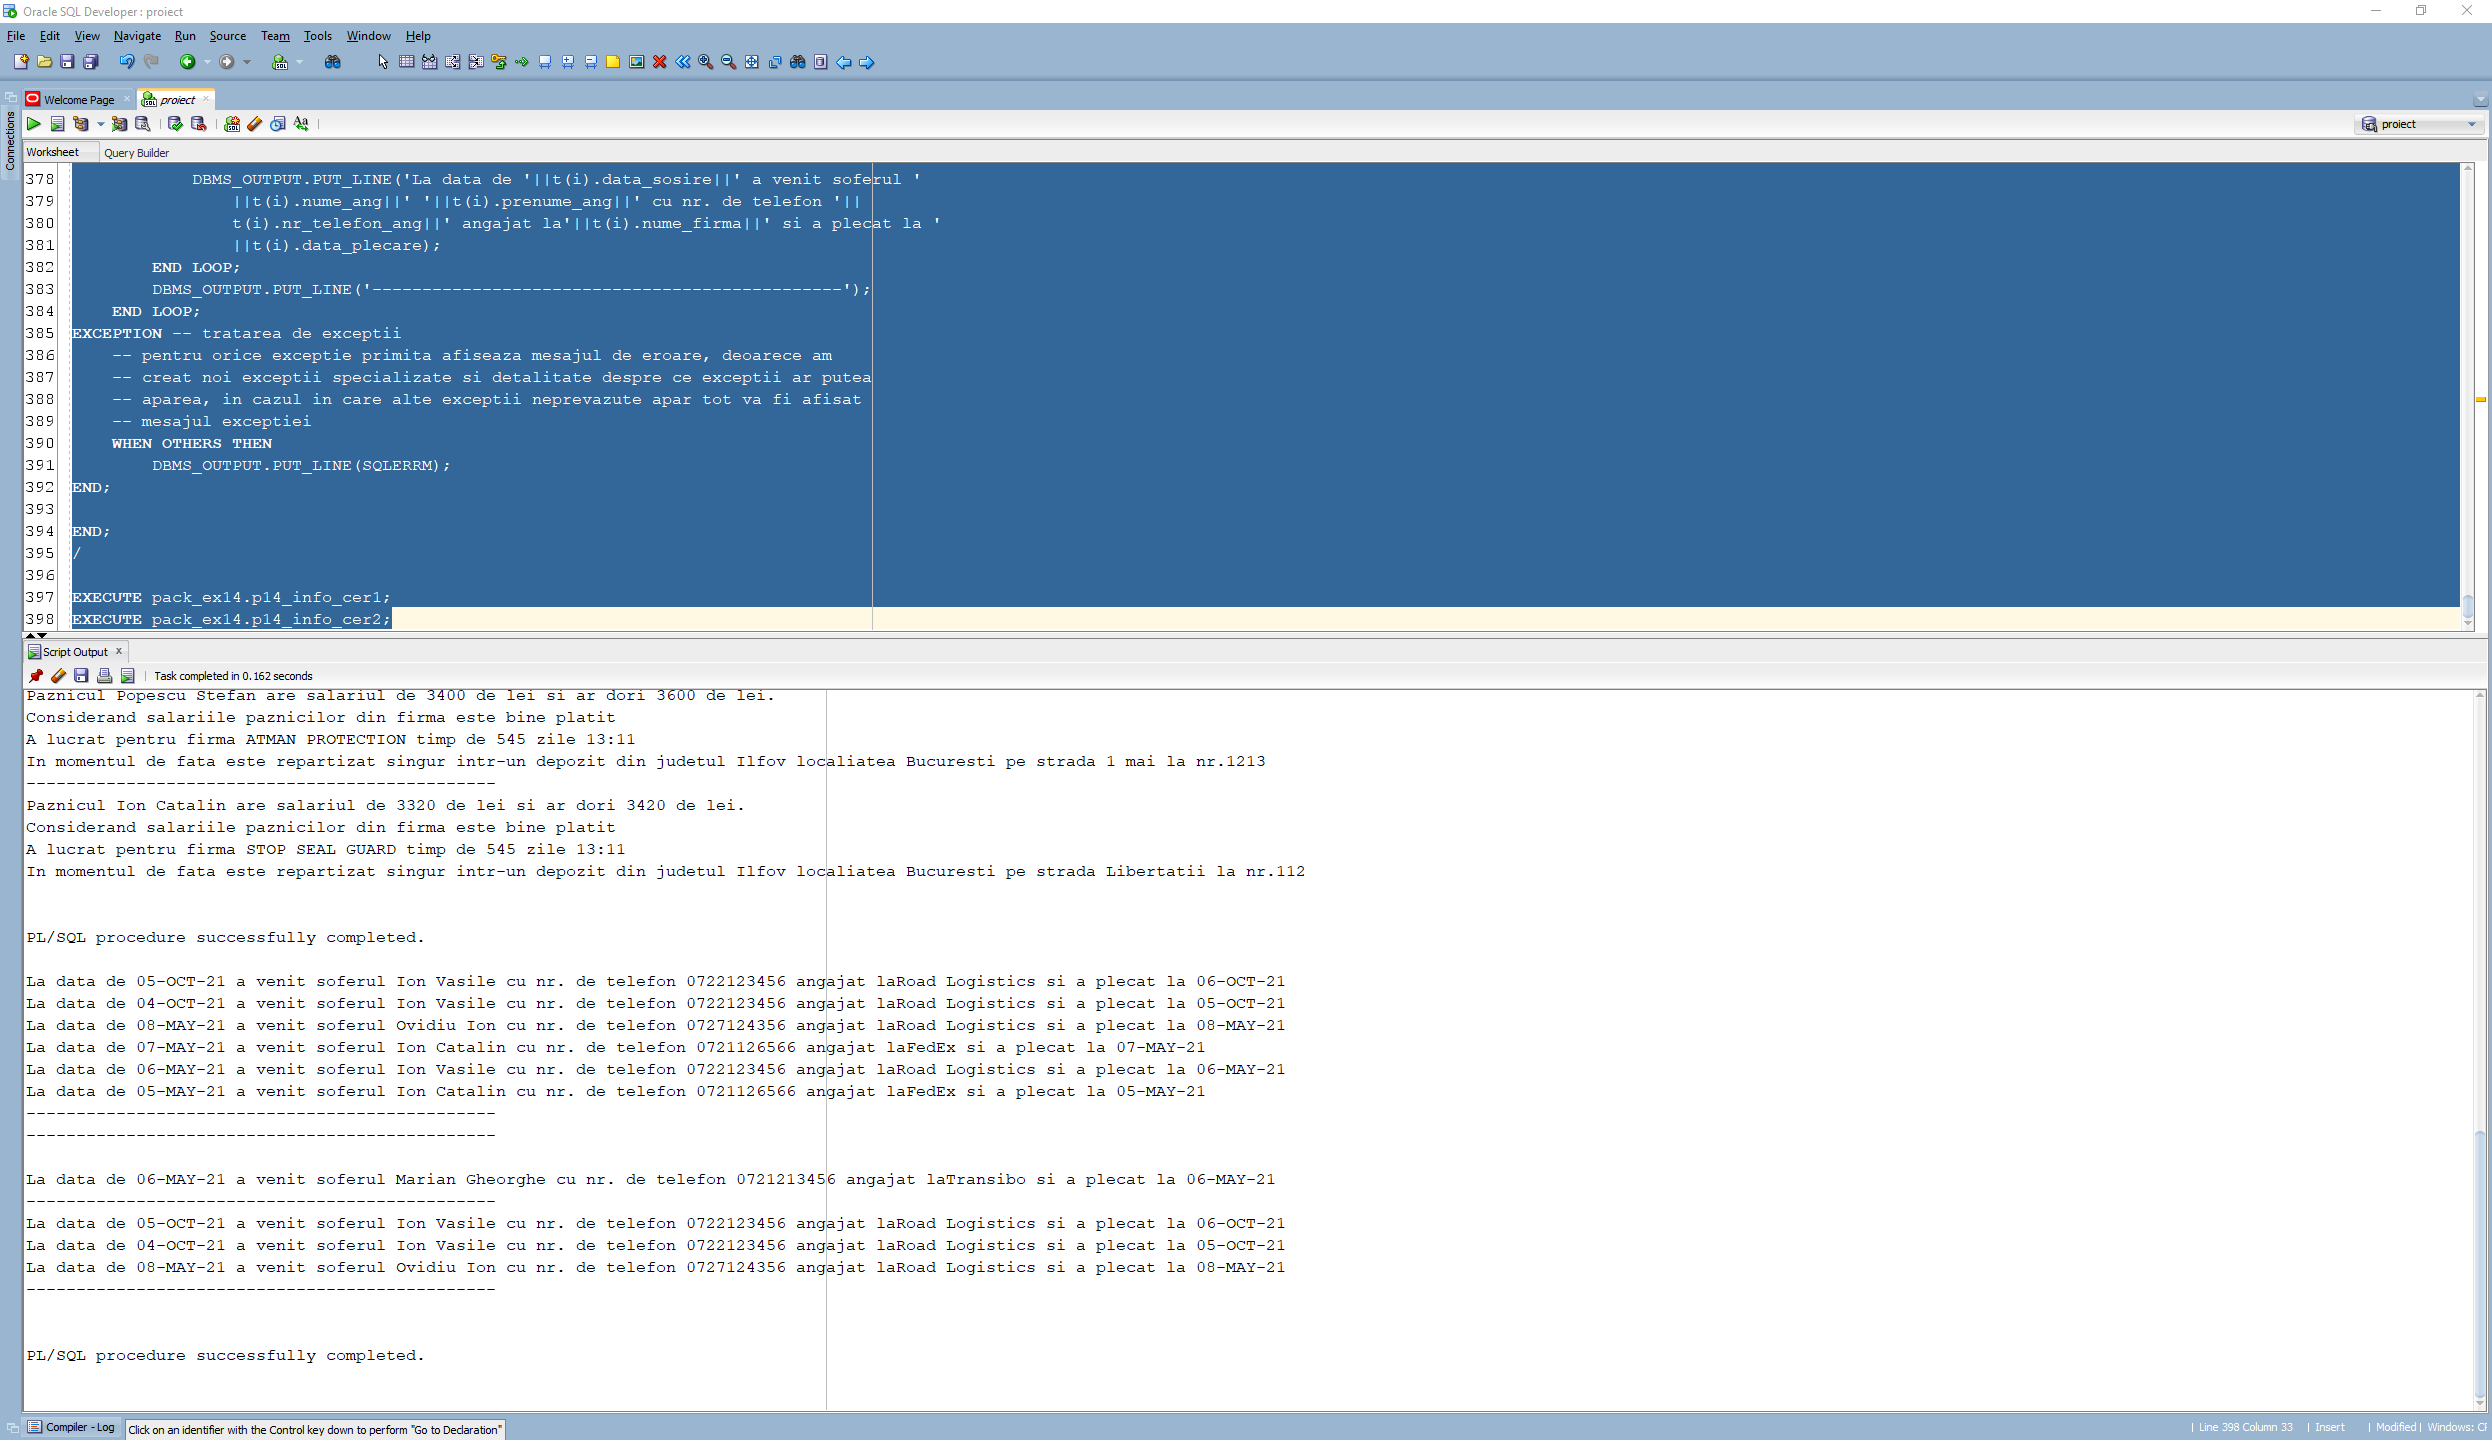
\includegraphics[width=\textwidth]{14_2.png}

\end{document}
